%%%%%
%%
%% Sample document ``thesis.tex''
%%
%% Version: v0.2
%% Authors: Jean Martina, Rok Strnisa, Matej Urbas
%% Date: 30/07/2008
%%
%% Copyright (c) 2008-2011, Rok Strniša, Jean Martina, Matej Urbas
%% License: Simplified BSD License
%% License file: ./License
%% Original License URL: http://www.freebsd.org/copyright/freebsd-license.html
%%%%%

% Available documentclass options:
%
%   <all `report` document class options, e.g.: `a5paper`>
%   withindex   - enables the index. New index entries can be added through `\index{my entry}`
%   glossary    - enables the glossary.
%   techreport  - typesets the thesis in the technical report format.
%   firstyr     - formats the document as a first-year report.
%   times       - uses the `Times` font.
%   backrefs    - add back references in the Bibliography section
%
% For more info see `README.md`
%\documentclass[withindex,glossary,techreport]{cam-thesis}
%\documentclass[withindex,glossary]{cam-thesis}
\documentclass[]{cam-thesis}

% Citations using numbers
\usepackage[sort&compress,numbers]{natbib}
%\usepackage[numbers]{natbib}
\usepackage{amsfonts}
\usepackage{amssymb}
\usepackage{xcolor}
\usepackage{setspace}

\usepackage{caption}
\usepackage{subcaption}
\usepackage[bottom]{footmisc}
\usepackage{tikz-cd} 
\usepackage{amsthm}
\usepackage{bbm}
\usepackage{mathrsfs}
\usepackage{verbatim}
\usepackage{alphalph}
\usepackage{yhmath}
\usepackage{mathtools}
\usepackage{listings}
\usepackage{courier} 

%\usepackage[toc]{appendix}
\usepackage{bookmark}

%\onehalfspacing

%%% Commands

\newtheorem{theorem}{Theorem}[section]
\newtheorem{lemma}{Lemma}[section]
\newtheorem{definition}{Definition}[section]
%\newtheorem*{remark}{Remark}

\newcommand*\circled[1]{\tikz[baseline=(char.base)]{
            \node[shape=circle,draw,inner sep=2pt] (char) {#1};}}

%%%%%%%%%%%%%%%%%%%%%%%%%%%%%%%%%%%%%%%%%%%%%%%%%%%%%%%%%%%%%%%%%%%%%%%%%%%%%%%%
%% Thesis meta-information
%%

%% The title of the thesis:
\title{Rare events and dynamics in non-equilibrium systems}

%% The full name of the author (e.g.: James Smith):
\author{Lukas Takaaki Kikuchi}

%% College affiliation:
\college{Churchill college}

%% College shield [optional]:
\collegeshield{CollegeShields/CUniNoText}

%% Submission date [optional]:
% \submissiondate{November, 2042}

%% You can redefine the submission notice [optional]:
% \submissionnotice{A badass thesis submitted on time for the Degree of PhD}

%% Declaration date:
\date{October, 2022}

%% PDF meta-info:
\subjectline{Soft condensed matter and statistical physics}
\keywords{non-equilibrium-physics}

%%% TODO to fix
\begin{comment}
	
Figures fixes:
[10:58, 28/11/2022] Ronojoy: Fig. 3.1 needs to be arranged better...perhaps increase the top panel ?
[10:58, 28/11/2022] Ronojoy: Or separate it out ?
[10:59, 28/11/2022] Ronojoy: The first figure is low on info content, so perhaps not needed at same scale ?
[10:59, 28/11/2022] Ronojoy: Fig. 3.3: the colorbar should be the same size of the colourplot, if that can be arranged.
[11:00, 28/11/2022] Ronojoy: Fig. 3.4: needs caption.
[11:01, 28/11/2022] Ronojoy: Fig. 3.5: perhaps use symbols, so that you do not have to use (red line) / (blue line) ...
[11:01, 28/11/2022] Ronojoy: Fig. 3.10 needs to be increased in size.
[11:02, 28/11/2022] Ronojoy: Generally for Figs in Chap 3: can you keep a consistent colormap please ?
[11:02, 28/11/2022] Ronojoy: Chapter 4 is quite compressed. Is this how you intended it to be ?


Have a thorough look on references.


You havent actually read through the thesis as well.


	
\end{comment}













%%%%%%%%%%%%%%%%








%\onehalfspacing

%%%%%%%%%%%%%%%%%%%%%%%%%%%%%%%%%%%%%%%%%%%%%%%%%%%%%%%%%%%%%%%%%%%%%%%%%%%%%%%%
%% Abstract:
%%
\abstract{%

The matter of this thesis is divided in two parts, both of which of are substantially different from the other, but nevertheless belong to disciplines that lie within the purview soft matter physics.

In the first part, we study the infinite-dimensional probability space of stochastic differential equations. In particular, we study the transition path ensemble (TPE), the set of transition paths between meta-stable states of It\^{o} diffusions. In the limit of vanishing diffusivity, the Freidlin-Wentzell action characterises the asymptotic character of the path-probability distribution over the TPE. We develop spectral Ritz methods to efficiently find minimisers of this action, and to construct quasipotentials of steady-state distributions, and we test our algorithm on a number of benchmark systems. To study the TPE in the finite temperature regime, we develop an MCMC algorithm to sample the infinite-dimensional space of transition paths, which we call the \textit{teleporter MCMC}. The algorithm was designed to efficiently sample the TPEs of It\^{o} diffusions with multiple competing transition channels, avoiding the issue of slow-mixing common to MCMC schemes. We concluded this part of the thesis by applying our MCMC method to study the temperature-dependence of the TPE. Using two model systems, we show that the dominant transition channel does not in general coincide with the most probable path of the path distribution, even in a low-to-intermediate temperature regime.

In the second part of this thesis we develop a general theory of the geometric mechanics of a broad class of microstructured continuum systems. Specifically, we consider systems with configuration spaces that are either Lie groups, or homogeneous spaces. We demonstrate that this theory, which we call a generalised geometric Cosserat theory (GGCT), can be seen as a unifying framework with which to study classical Cosserat systems, and numerous non-classical variations. As a paradigmatic example we first study the Cosserat rod model, we identify its configuration space as a curve in $SE(3)$, the Lie group of translations and rotations on Euclidean space, and use the Lie algebra-Lie group correspondence to relate its configuration to curves in the Lie algebra. Using the Euler-Poincar\'e theorem we then proceeded to formulate the dynamics of the Cosserat rod on the dual Lie algebra. The resulting kinodynamical - kinematic and dynamic - theory of the Cosserat rod is defined completely on the trivialisation of the tangent bundle of $SE(3)$, the Lie algebra $\mathfrak{se}(3)$. We then constructed the GGCT by extrapolating these above steps to systems with generalised configuration spaces. In the final chapter of this thesis, we constructed geometric numerical integrators designed to preserve the qualitative features of the system geometry.

}

%%%%%%%%%%%%%%%%%%%%%%%%%%%%%%%%%%%%%%%%%%%%%%%%%%%%%%%%%%%%%%%%%%%%%%%%%%%%%%%%
%% Acknowledgements:
%%
\acknowledgements{%
I would like to first of all thank my supervisor, Ronojoy Adhikari, for his guidance and creativity in conceptualising our research together. I have grown immensely as a research scientist throughout my doctoral studies, and this is in very large part thanks to him.

Secondly, I am immensely grateful for the persistent support and mentorship of Julian Kappler, who was my frequent collaborator throughout my studies.  

I would also like to thank my secondary supervisor Mike Cates, for his advice, willingness to proofread my manuscripts and interesting discussions. Additionally, I would like to give thanks and appreciate the soft matter group, for their conviviality and support. 

Lastly, I would like to thank my friends, who are my family.

 % I would like to thank my supervisor, Ronojoy Adhikari, and his creativity and 
 % Mike Cates, Julian Kappler
 
 % Lastly, Lia Yolanda Ishan, Yedzin, Soogun
 % Perhaps one day we will all live in a commune
 % To the roll of a dice
 
 % for picking me up when
 
 % The one who rolls the dice up above.
 
% their love makes me everyday.
 
}

%%%%%%%%%%%%%%%%%%%%%%%%%%%%%%%%%%%%%%%%%%%%%%%%%%%%%%%%%%%%%%%%%%%%%%%%%%%%%%%%
%% Dedication:
%%
\dedication{%
To my friends.
%To me, myself and I, but most of all my friends.
%To me, myself and I, but most of all, to my friends.
%To me, myself and I.\footnote{But most of all, to my friends.}

  %To me, myself and I, but mostly my friends.
  % To me, myself and I, but most-
  % To the roll of a dice
  % To the dice roll
  % To the dice roller
}

%%%%%%%%%%%%%%%%%%%%%%%%%%%%%%%%%%%%%%%%%%%%%%%%%%%%%%%%%%%%%%%%%%%%%%%%%%%%%%%%
%% Glossary [optional]:
%%
%\newglossaryentry{HOL}{
%    name=HOL,
%    description={Higher-order logic}
%}



%%%%%%%%%%%%%%%%%%%%%%%%%%%%%%%%%%%%%%%%%%%%%%%%%%%%%%%%%%%%%%%%%%%%%%%%%%%%%%%%
%% Contents:
%%
\begin{document}



%%%%%%%%%%%%%%%%%%%%%%%%%%%%%%%%%%%%%%%%%%%%%%%%%%%%%%%%%%%%%%%%%%%%%%%%%%%%%%%%
%% Title page, abstract, declaration etc.:
%% -    the title page (is automatically omitted in the technical report mode).
\frontmatter{}



%%%%%%%%%%%%%%%%%%%%%%%%%%%%%%%%%%%%%%%%%%%%%%%%%%%%%%%%%%%%%%%%%%%%%%%%%%%%%%%%
%% Thesis body:
%%


%%%%%%%%%%%%%%%%%%%%%%%%%%%%%%%%%%%%%%%%%%%%%%%%%%%%%%%%%%%%%%%%%%%%%%%%%%%%%%%%
%% PART I : Introduction
%%%%%%%%%%%%%%%%%%%%%%%%%%%%%%%%%%%%%%%%%%%%%%%%%%%%%%%%%%%%%%%%%%%%%%%%%%%%%%%%



\chapter*{Introduction}
\addcontentsline{toc}{chapter}{Introduction}

This thesis explores two distinct topics. The first part concerns itself with the study of transition events in stochastic differential equations, both in regimes where these are ubiquitous as well as rare. The second part develops a geometrical theory of Cosserat materials \citep{cosseratTheoryDeformableBodies1909}, and further a generalised framework for studying continuum systems with configurations taking value in Lie groups or homogeneous spaces. Whilst substantially different, the two parts of this thesis do share a common trait in that they explore the geometry of spaces that possess an infinite-dimensional character. In essence, the research we present in the first part of the thesis quantitatively and qualitatively investigates the concentration of path-probability measures, defined over the infinite-dimensional space of stochastic transition paths. In the second part of this thesis, we consider systems with infinite degrees-of-freedom; that is, the systems are Lie group-valued \textit{manifolds} and we construct a general kinematic and dynamical theory of such systems in terms of their intrinsic geometry. Below we will separately introduce the two parts of this thesis.

\section*{\large Global methods for sampling rare diffusive events}
\addcontentsline{toc}{section}{Global methods for sampling rare diffusive events}

Randomness is important on all scales in nature, and is ubiquitous in the mesoscopic scales of soft matter physics. Rich phenomena in physical, chemical and biological systems often emerge out of the interplay between stochastic and deterministic forces, as for example in the nucleation of solids, the conformational changes in biomolecules, or shifts in ecological balance \citep{faccioliDominantPathwaysProtein2006a, demarcoPhaseTransitionModel2001a, gardnerConstructionGeneticToggle2000a, mangelBarrierTransitionsDriven1994a, wolynesNavigatingFoldingRoutes1995a, huangMolecularMathematicalBasis2012a, paninskiMostLikelyVoltage2006a, noltingBallsCupsQuasipotentials2016a, leeFindingMultipleReaction2017a}. Mathematically, many systems of this kind can be modelled as overdamped Langevin dynamics, otherwise known as It\^{o} diffusions \citep{kampenStochasticProcessesPhysics2011a, gardinerStochasticMethodsHandbook2010a, riskenFokkerPlanckEquationMethods2012a, bharucha-reidElementsTheoryMarkov2012a}. The stochastic trajectories of such random processes tend to concentrate around attractors of the dynamics in state-space, determined by the drift-field, which for gradient dynamics correspond to energetic minima. The influence of the stochastic forces renders the otherwise stable fixed points meta-stable, such that transitions between points or regions of meta-stability have finite probability. The set of all such transition paths between given meta-stable states is known as the transition path ensemble (TPE) \citep{bolhuisTransitionPathSampling2002a}. In Langevin models, the configuration of the system is often a reaction coordinate, and the characteristic pathways and rate constants of transition events are the main object of study \citep{dellagoCalculationReactionRate1999a, arjunUnbiasedAtomisticInsight2019, geisslerAutoionizationLiquidWater2001, carterConstrainedReactionCoordinate1989, laioEscapingFreeenergyMinima2002, bestMicroscopicInterpretationFolding2016, arjunUnbiasedAtomisticInsight2019}.

However transition events often occur on time-scales much larger than those of the dynamics itself \citep{petersReactionRateTheory2017, bolhuisTransitionPathSamplinga, grafkeLongTermEffects2017}. For example, the molecular dynamics of proteins are orders of magnitude smaller than the time-scale under which it unfolds \citep{veitshansProteinFoldingKinetics1997a}. In other words, transitions are \textit{rare events} for many relevant systems. Where analytical methods are intractable, numerical methods must be used to sample the transition path ensemble. However, it is in general not feasible to sample the TPE using standard stochastic integrators or molecular dynamics simulatons, due to the disparate time-scales of the target sample space and the dynamics. The study of the TPE must be approached via other means.

One such method is through the large deviation theory of Freidlin, Wentzell and Graham \citep{wentzellSmallRandomPerturbations1970, graham1987macroscopic}, which studies the TPE in the limit of vanishing noise, the so-called \textit{Freidlin-Wentzell limit}. The exponential scaling of transition rates in the noise-strength parameter can then be estimated by finding the global minimiser of an action functional. This minimiser, known as the \textit{instanton}, is the `least unlikely` pathway that the system will take in transition events, and any deviation from this path is exponentially suppressed in probability. However the limit of vanishing noise is unrealistic for many real physical systems, and some qualitative features of the transition paths may only emerge at finite temperatures \cite{pinskiTransitionPathsMolecules2010b}. In these regimes, sampling techniques must be used to sample the functional probability distribution over the TPE. Prominent examples of sampling methods are the \textit{transition path sampling} (TPS) \citep{dellagoTransitionPathSampling1998a, dellagoCalculationReactionRate1999a, dellagoEfficientTransitionPath1998, bolhuisTransitionPathSamplinga, bolhuisTransitionPathSampling2002a} and \textit{forward flux sampling} (FFS) \citep{escobedoTransitionPathSampling2009, allenForwardFluxSamplingtype2006, hussainStudyingRareEvents2020}. % Could add some stuff about the challenge of sampling multiple transiiton pathways.

In this first part of the thesis we offer some contributions to the study of the transition path ensemble of general overdamped Langevin systems, in both the Freidlin-Wentzell limit and at finite temperatures. In Ch.~\ref{ch:Ritz methods for Freidlin-Wentzel-Graham actions} we develop global methods of numerically minimising action functionals. The resulting method can be used to compute the \textit{quasi-potential} of general overdamped Langevin equations, which is a WKB-approximation of its steady-state distribution \citep{graham1987macroscopic, maier1996scaling, ludwig1975persistence}, as well the Freidlin-Wentzell instanton. 

In Ch.~\ref{ch:Monte Carlo methods in Path Spaces} we move on to consider transition path ensembles at finite temperatures. We begin with a survey of recent developments in the field of functional MCMC methods. We explain in detail the \textit{preconditioned Nicolson-Crank} algorithm \citep{cotterMCMCMethodsFunctions2013a, beskosMCMCMETHODSDIFFUSION2008a, hairerAnalysisSPDEsArising2005a, hairerAnalysisSPDEsArising2007a, hairerSpectralGapsMetropolis2014a}, which is an instance of an infinite-dimensional MCMC scheme. We apply this method to sample the TPE by expanding stochastic trajectories in the \textit{Kosambi-Karhunen-Lo\`eve} basis \citep{kosambiParallelismPathspaces2016, karhunenUeberLineareMethoden1947, loeveProbabilityTheory1977a} of the corresponding drift-less free diffusion system, which is a method by which Gaussian stochastic processes can be expressed in terms of an infinite series of independent Gaussian random numbers. In doing so, we find that the spectrum of - \textit{non-Gaussian} - Langevin processes possess a band-structure, where only the lower-frequency band have non-trivial statistics; that is, the infinite-dimensional space of stochastic transition paths, of a general overdamped Langevin system, admits an \textit{effective} finite-dimensionalisation. We utilised this band-separation to modify and improve the autocorrelation times of the pCN. The main result of this chapter is the construction of the \textit{teleporter MCMC} (TMC), which is a combination of the pCN method and a set of independence samplers. The latter are constructed, using a semi-classical expansion of the path-probability distribution around the locally most-probable paths of the TPE. This in turn allows the MCMC to `teleport' between dominant transition channels. The teleporter MCMC was designed to deal with the issue of \textit{slow mixing} \citep{holdenMixingMCMCAlgorithms2019}, which is a common problem faced by MCMC methods that sample target distributions where the local maxima lack mutual support in the sample space. In the context of transition paths, we have that methods like the pCN will in general fail to mix between multiple transition channels in a single run, thus generating a biased sample. The TMC circumvents this problem by allowing the Markov chain to intermittently teleport between the transition channels, using the independence samplers. Finally, a section in this chapter is also dedicated to discuss the relation between the mathematical notion of a path-probability measure (or \textit{law}), and the infinite-dimensional path-probability densities (and path integrals) which are ubiquitous in physics. We show that the latter, which are often understood by mathematicians and physicists alike to be of dubious mathematical rigour, can be recontextualised and even be made rigorous by understanding how they relate to well-defined mathematical objects.

In Ch.~\ref{ch:Diffusivity dependence of transition paths}, the final chapter of this part of the thesis, we apply and extend the methods of the previous chapter to study the concentration of competing transition channels in the TPE, as a function of temperature. Using two model systems, we show that the dominant transition channel does not in general coincide with the most probable path of the path distribution, even in a low-to-intermediate temperature regime. We construct a semi-analytical approximation of the TPE as mixture of Gaussian measures using the semi-classical expansion of the path-probability distribution. We then apply this approximate probability measure to estimate the relative probability of competing transition channels. We verify the validity of these estimators using the MCMC methods developed in the previous chapter. We also demonstrate, using the model systems, that the interplay between fluctuations and drift can lead to the unintuitive result of energetically unfavourable transition channels dominating over the energetically favourable channels.

\section*{\large Geometric mechanics of microstructured soft matter}
\addcontentsline{toc}{section}{Geometric mechanics of microstructured soft matter}

Solids and liquids are generally viewed from a macroscopic perspective as continuous materials that can continuously deform in time. In \textit{infinitesimal strain theory} \citep{landauTheoryElasticityVolume1986}, the deformations are assumed small enough to not significantly affect the overall shape. However, this assumption does not hold soft matter materials, that are often highly deformable \citep{volokhMechanicsSoftMaterials2019}. Furthermore, beyond the spatial extension of the continuum body, many systems relevant to soft matter physics \citep{krishnaswamyCosserattypeModelRed1996, rangamaniSmallScaleMembrane2014, sackBiologicalTissueMechanics2016, zhangModelingSimulationComplex2019, corazzaUnravelingLoopingEfficiency2022} also have internal degrees of freedom, which we call \textit{microstructure}. The classical account of microstructured continuum mechanics was given in the seminal work of the Cosserat brothers \cite{cosseratTheoryDeformableBodies1909} in 1909. There, they introduced the notion of a what is now called a \textit{Cosserat material}: A continuum body $\mathcal{M} \subset \mathbb{E}^3$, where there are $n$ deformable vectors, known as \textit{directors}, attached at each point $p \in \mathcal{M}$. For such systems, they derived the mechanical equation of motion of the spatial continuum body $\mathcal{M}$ as well as the $n$ director-fields on $\mathcal{M}$. This formalism is applicable to many physical systems. The shell of a cell membranes can be modelled as a mid-surface in Euclidean space, with a single director that point towards and away from the inner and outer shell boundaries respectively \citep{krishnaswamyCosserattypeModelRed1996, rangamaniSmallScaleMembrane2014}. The corresponding one-dimensional model is the Cosserat rod, which consists of a center-line curve and two director fields representing the deformation of its cross-section. Such models are prominently used in soft robotics \citep{rendaDiscreteCosseratApproach2018, graziosoGeometricallyExactModel2019, rendaDiscreteCosseratApproach2016, caasenbroodEnergyShapingControllersSoft2022, boyerMacrocontinuousComputedTorque2006, boyerMacrocontinuousDynamicsHyperredundant2012, rendaDynamicModelMultibending2014, verlSoftRoboticsTransferring2015, naughtonElasticaCompliantMechanics2021}, the modelling of muscles and ligaments \citep{sackBiologicalTissueMechanics2016, zhangModelingSimulationComplex2019}, and three-dimensional Cosserat models are frequently used in material science \citep{stefanouCosseratApproachLocalization2017,
forestCosseratModellingSize2000,
altenbachCosseratMedia2013,
ebrahimianNumericalStudyInterface2021,
mohanFrictionalCosseratModel1999,
koteraCosseratContinuumTheory2000,
stefanouThreedimensionalCosseratHomogenization2008,
onckCosseratModelingCellular2002,
iesanDeformationPorousCosserat2011}. There are also many examples in nature of active filaments \citep{moultonElasticSecretsChameleon2016, oliveriTheoryDurotacticAxon2021, kierTonguesTentaclesTrunks1985, moultonMultiscaleIntegrationEnvironmental2020}, which are slender rods \citep{kirchhoffUeberGleichgewichtUnd1859, dillKirchhoffTheoryRods1992, gorielyNonlinearDynamicsFilaments2000} that have internal configurations \citep{kaczmarskiActiveFilamentsCurvature2022}.

In contrast to rigid bodies, which we can only subject to external forcing, a continuum system admits the notion of a \textit{stress}. That is, the dynamics of continua are \textit{constitutive}, and force fields that arise due to internal stresses are functions not of the deformations themselves, but its rate-of-change. For continua without microstructure, connections can be made between continuum mechanics and standard concepts in Riemannian geometry. For example, the rate of deformation can be related to a Lie derivative of the Riemannian metric \citep{marsdenMathematicalFoundationsElasticity1994}. As the relevant dynamical quantities for constitutive continuum mechanics are defined in terms the derivatives of their deformations, it may be convenient to parameterise its mechanics in terms of its intrinsic geometry. An extensive literature on such geometrisations exist for the case of systems without microstructure \citep{marsdenMathematicalFoundationsElasticity1994, wangIntroductionRationalElasticity1973, wangGeometricStructuresSimple1967, greenMechanicsNonlinearMaterials1957, lublinerMethodVirtualPower, nollMathematicalTheoryMechanical1958}. Though Cosserat theory, and microstructured models in general, are used widely, there is no extensive literature on equivalent geometrised theories for such systems. In \citep{yamaokaContinuumDynamicsVector2010} a formulation analogous to the Riemannian approach applied to Cosserat media, using a vector bundle construction.

However there is a more natural geometrical formulation for Cosserat materials. Namely, we can identify a \textit{Lie group structure} in their kinematic configuration spaces. Such approaches have been exemplified previously in \citep{giusteriSimulationViscoelasticCosserat2021, giusteriImportanceEffectivenessRepresenting, chirikjianStochasticElasticaExcludedVolume2008, holmMatrixGstrands2014}. There, a Cosserat rod with a rigid-body cross-section was kinematically parameterised as a curve in $SE(3)$, the Lie group of translations and rotations on three-dimensional Euclidean space. This formulation naturally lends itself to formulating the kinematics and dynamics, which we will abbreviate as \textit{kinodynamics} \citep{donaldKinodynamicMotionPlanning1993, donaldProvablyGoodApproximation1995} henceforth, in terms of the corresponding \textit{Lie algebra} $\mathfrak{se}(3)$, using the Lie group-Lie algebra correspondence. The resulting kinodynamic equations of motion encapsulate the intrinsic geometry of both the external and internal degrees of freedom of the Cosserat rod.

In the second part of this thesis, we will construct a general theory of the geometric mechanics of a broad class of microstructured continuum systems. Specifically, we will consider continua with configuration spaces that are Lie groups, as well as \textit{homogeneous spaces}\footnote{See Sec.~\ref{sec:Mathematical preliminaries} for a definition.}. We call these \textit{generalised Cosserat systems}, and we will refer to our theoretical study of this class of systems as a \textit{generalised geometric Cosserat theory} (GGCT). This class encompasses and goes beyond the entire suite of possible Cosserat models. Mathematically, we will show that the GGCT can be seen as a field theory, defined on arbitrary topological base manifolds, and takes values in general Lie groups or homogeneous spaces. The kinodynamic formulation of these fields are then derived in terms of the Lie algebraic structure of their configuration spaces. In numerical simulations, the benefit of our geometric approach is that constitutive dynamics can now be formulated without the need of triangulating the configurational manifold of the system, otherwise known as finite-element methods (FEM) \citep{hughesFiniteElementMethod2012}. 

In Ch.~\ref{sec:geometry introduction} we will introduce the classical theory of Cosserat materials. In particular, we focus on the Cosserat rod, which we will treat carefully in the subsequent chapter. We will also introduce the necessary mathematical formalism required for the GGCT. These mathematical preliminaries will also serve as an introduction to the theory of sub-manifolds of Lie groups and homogeneous spaces.

In Ch.~\ref{ch:Cosserat rods} we study in detail the Cosserat rod and the filament, the corresponding non-microstructured system. As in \citep{giusteriSimulationViscoelasticCosserat2021, giusteriImportanceEffectivenessRepresenting, chirikjianStochasticElasticaExcludedVolume2008, holmMatrixGstrands2014}, we parameterise the Cosserat rod as a curve in $SE(3)$, and use the Lie group-Lie algebra map to construct a corresponding curve in the Lie algebra $\mathfrak{se}(3)$. We also provide additional mathematical context, identifying the Lie algebraic kinematic configuration as the \textit{Maurer-Cartan form} (MC), a Lie algebra-valued $1$-form. The kinematic equations of motion are then found as a result of the \textit{Maurer-Cartan equations}, which enforce the integrability of the MC form. We then derive the conservative and constitutive dynamics of the Cosserat rod using the \textit{Euler-Poincar\'e theorem} \citep{marsdenIntroductionMechanicsSymmetry2013, marleHenriPoincareNote2013a}. By constructing a generalised Lagrange-D'Alembert principle, we then derive generalised non-conservative dynamics. We will conceptualise the filament as a kinematically constrained Cosserat rod, analogous to forming a homogeneous space from the quotient $G/H$, of a Lie group $G$ and a Lie subgroup $H \subset G$. Drawing on the methods already developed for the Cosserat rod, we then derive the full kinodynamic equations of motion of the filament. In addition to the geometrised theory we provide here, we will also derive and specify some physical models as applications of our theory.

In Ch.~\ref{ch:Geometric continuum mechanics on homogeneous configuration spaces} we present and derive (in that order) the generalised geometric Cosserat theory. The theory is largely constructed analogously as a generalisation of the treatment in Ch.~\ref{ch:Cosserat rods}, and conceptually we use the Cosserat rod and filament as an pedagogical device to understand generalised Cosserat systems with Lie group- and homogeneous configuration spaces respectively. We conclude this chapter with a chapter on applications of the GGCT. We considered the classical cases of the Cosserat rod, surface and body, as well as Cosserat rod on spheres and Minkowski space. To illustrate the connection between the GGCT and field theories, we also applied it to study the $O(n)$ non-linear $\sigma$ field theory (NLSM) \citep{ketovQuantumNonlinearSigmaModels2013}. Using our example systems, we aim to demonstrate the generality of the programme, but also emphasise the its relative ease-of-use. 

Finally, in Ch.~\ref{ch:Geometric numerical integrators} we refine the GGCT for numerical applications. We begin by observing that the right-hand sides of the kinodynamic equations of motion can be identified as a Lie algebra action on itself. This allows us to formulate \textit{geometric integrators}, designed to qualitatively preserve geometric features in numerical simulations. We contextualise our work as an application of \textit{Lie group integration} theory  \citep{celledoniIntroductionLieGroup2014c, owrenLieGroupIntegrators2016, iserlesLiegroupMethods2005, celledoniLieGroupIntegrators2022a}, applied in the infinite-dimensional setting of continuum systems. We apply our geometric integrators to show that they successfully outperform standard PDE integrators in preserving the geometric features of the system.




\begin{comment}
Lit review:

\citep{parkCosseratMicromechanicsHuman1986, ivanovaNewTheoryCosserat2022, pariaUnifiedTheoryMechanics1978, ivanovaModelingPhysicalFields, gorielyRodTheoryLiquid2022}


% modelling of muscles and ligaments

\citep{stefanouCosseratApproachLocalization2017}, polycrystalline \citep{forestCosseratModellingSize2000} and composite materials \citep{altenbachCosseratMedia2013}, granular and powder-like materials \citep{ebrahimianNumericalStudyInterface2021, mohanFrictionalCosseratModel1999, koteraCosseratContinuumTheory2000}, masonries \citep{stefanouThreedimensionalCosseratHomogenization2008}, cellular \citep{onckCosseratModelingCellular2002} or porous media and foams \citep{iesanDeformationPorousCosserat2011}, bones \citep{parkCosseratMicromechanicsHuman1986}, liquid
crystals \citep{epsteinContinuousDistributionsInhomogeneities2001, gorielyRodTheoryLiquid2022}, as well as electromagnetic and ferromagnetic media \citep{ivanovaNewTheoryCosserat2022, pariaUnifiedTheoryMechanics1978, ivanovaModelingPhysicalFields}

\citep{krishnaswamyCosserattypeModelRed1996, rangamaniSmallScaleMembrane2014}

 many systems relevant to soft matter physics 

\citep{ericksenLiquidCrystalsCosserat1974}

soft robotics 

cell membranes \citep{krishnaswamyCosserattypeModelRed1996, rangamaniSmallScaleMembrane2014}

biological tissue \citep{sackBiologicalTissueMechanics2016, zhangModelingSimulationComplex2019}

soft matter: 

active filaments \citep{laskarBrownianMicrohydrodynamicsActive2015, laskarFilamentActuationActive2017, kaczmarskiActiveFilamentsCurvature2022, pandeyFlowinducedNonequilibriumSelfassembly2016}

filaments \citep{gazzolaForwardInverseProblems2018, goldsteinFrontProgagationPearling1996, goldsteinViscousNonlinearDynamics1998, goldsteinNonlinearDynamicsStiff1995}

Many applicaitons in engineering and continuum mechanics:
 soils \citep{stefanouCosseratApproachLocalization2017}, polycrystalline \citep{forestCosseratModellingSize2000} and composite materials \citep{altenbachCosseratMedia2013}, granular and powder-like materials \citep{ebrahimianNumericalStudyInterface2021, mohanFrictionalCosseratModel1999, koteraCosseratContinuumTheory2000}, masonries \citep{stefanouThreedimensionalCosseratHomogenization2008}, cellular \citep{onckCosseratModelingCellular2002} or porous media and foams \citep{iesanDeformationPorousCosserat2011}, bones \citep{parkCosseratMicromechanicsHuman1986}, liquid
crystals \citep{epsteinContinuousDistributionsInhomogeneities2001, gorielyRodTheoryLiquid2022}, as well as electromagnetic and ferromagnetic media \citep{ivanovaNewTheoryCosserat2022, pariaUnifiedTheoryMechanics1978, ivanovaModelingPhysicalFields}

\end{comment}




\part{Global methods for sampling rare diffusive events}

\chapter{Ritz methods for Freidlin-Wentzel-Graham actions} \label{ch:Ritz methods for Freidlin-Wentzel-Graham actions}

\section{Introduction}

The theory of Freidlin and Wentzell \citep{ventsel1970small}
gives asymptotic probability estimates of rare events in dynamical
systems perturbed by small noise \citep{bolhuis2002transition, allen2005sampling, allen2009forward, ebener2019instanton}.
Specifically, Freidlin-Wentzell theory yields estimates of the stationary
distributions and mean first-passage times. Both these quantities
are determined, in turn, by the asymptotic estimate of the probability
of a stochastic trajectory to not deviate from a smooth path by more
than a given amount in a given interval of time. The key result of
Freidlin and Wentzell is that the limiting form of this probability,
for small noise and small deviations, is given by a non-negative functional
of the smooth path. This functional is the Freidlin-Wentzell action
and its minimum, for fixed initial and terminal states, determines
both the stationary distributions and first-passage times. The smooth
path minimising the action is often called the Freidlin-Wentzell instanton.
The theory is applicable to dynamical systems of both gradient and
non-gradient character and can so be used to study a wide variety
of equilibrium and non-equilibrium systems modelled by Itô diffusions
\citep{paninski2006most,huang2012molecular, bouchet2016generalisation, maier1996scaling, wolynes1995navigating, nolting2016balls, mangel1994barrier, gardner2000construction, demarco2001phase, nelson1987stochastic}.

Determining the minimum of the Freidlin-Wentzell action is a problem
in the calculus of variations. The Euler-Lagrange equations provide
the necessary conditions for extrema of variational problems and,
unsurprisingly, have been the basis of the large literature devoted
to the numerical computation of Freidlin-Wentzell instantons \citep{weinan2002string,paninski2006most,heymann2008geometric,grafke2017long}.
There exists, however, an alternative ``direct'' route for the solution
of variational problems in which the functional is reduced, through
finite-dimensional parametrizations of paths, to a multivariate function
and then extre\textcolor{black}{mised by appropriate multivariate
optimisation methods \citep{gelfand2012calculus,kantorovich1958approximate}.
To the best of our knowledge, the first use of the direct method for
the Freidlin-Wentzell action, discretised by finite-differences, appears
in the work of Weinan, Ren and Vanden-Eijnden \citep{weinan2004minimum}.} 

Here we combine the direct method with a Ritz discretisation \citep{ritz1909uber,gelfand2012calculus,kantorovich1958approximate}
to minimize the Freidlin-Wentzell action. We analyse paths in a spectral
basis of Chebyshev polynomials and use spectral quadrature to express
the action as a multivariate function of the basis coefficients. Nonlinear
optimisation is used to obtain coefficients that give the least action
from which the instanton is synthesised in the spectral basis.\textcolor{black}{{}
For minimisation over paths regardless of their duration, this procedure
is especially effective when applied to a reparametrisation-invariant
on-shell form of the action that follows from the time-translational
invariance of the Lagrangian. This generalises the scalar work functional
of Olender and Elber (for gradient dynamics) and the geometric action
of Heyman and Vanden-Eijnden} \citep{vanden2008geometric} (for non-gradient
dynamics). Our method is efficient enough to robustly sample the logarithm
of the asymptotic estimate of the stationary distribution, \emph{i.e.
}the quasipotential, avoiding the alternative, but numerically delicate,
route of solving the Hamilton-Jacobi equation \citep{cameron2012finding,yang2019computing,dahiya2018ordered}.
Our method is simple to use, converges rapidly, and is applicable
to both equilibrium and non-equilibrium problems. Its implementation
is freely available on GitHub as the open-source Python library PyRitz. 

The remainder of this chapter is organized as follows. In the next section,
we recall key results of Freidlin-Wentzell theory from dual perspectives
of Itô stochastic differential equations and the corresponding Fokker-Planck
equations.\textcolor{black}{{} Sec.~\ref{sec:Minima-of-the-action}
we present the derivation of the on-shell form of the Freidlin-Wentzell
action in a manner reminiscent of the Routh reduction procedure in
classical mechanics and explain its relation to the scalar work and
the geometric action. }In Sec.~\ref{sec:direct-method} we describe
the direct method for the minimisation of functionals, the Chebyshev
spectral basis in which we construct smooth paths, the spectral quadrature
rule we use to evaluate the action, and the multivariate non-linear
optimisation methods we employ to find the minimum. In Sec.~\ref{sec:pyritz-applications}
we apply the direct method to three well-known diffusion processes
and demonstrate convergence in each case. 

A particular achievement of our approach is its relatively facile
ability to calculate quasipotentials. This can be done with a sufficiently
high density of sample points to construct effectively continuous
maps of the quasipotential, which we do here for the same set of benchmark
problems. We conclude with a discussion on extending the method to
degenerate diffusion processes, systems with inertia and to the stochastic
dynamics of fields. 

\section{Large deviation theory} \label{sec:fwtheory}

We consider the autonomous dynamics of a $d$-dimensional coordinate
$X=(X^{1},\ldots,X^{d})$ in $\mathbb{R}^{d}$ perturbed by configuration-dependent
noise of intensity $\sqrt{\varepsilon}$ described by the Itô diffusion
equation \citep{oksendalStochasticDifferentialEquations2003, shreveStochasticCalculusFinance2005}
\begin{equation}
dX^{\mu}=a^{\mu}(X)dt+\sqrt{\varepsilon}\sigma_{\nu}^{\mu}(X)dW^{\nu}\label{general ito diffusion}
\end{equation}
governing the stochastic trajectory $X(t)$, where $a^{\mu}(X)$ is
the drift vector, $\sqrt{\varepsilon}\sigma_{\nu}^{\mu}(X)$ is the
volatility, $W^{\nu}(t)$ is a $d$-dimensional Wiener process and
repeated indices are summed over.  Eq.~\ref{general ito diffusion} is also often referred to as an \textit{overdamped Langevin equation}.

The transition probability density
of the process, $P_{1|1}(x,t|x_{0})=P(X(t)=x|X(0)=x_{0})$, obeys
the Fokker-Planck equation $\partial_{t}P(x|x_{0})=\mathcal{L}P(x|x_{0})$
where the Fokker-Planck operator is

\emph{
\begin{equation}
\begin{aligned}\mathcal{L}(x) & =-\frac{\partial}{\partial x^{\mu}}a^{\mu}(x)+\frac{\varepsilon}{2}\frac{\partial^{2}}{\partial x^{\mu}\partial x^{\nu}}b^{\mu\nu}(x)\end{aligned}
\label{eq:fokker-planck}
\end{equation}
}and \textbf{$b^{\mu\nu}(x)=\sigma_{\lambda}^{\mu}(x)\sigma_{\sigma}^{\nu}(x)\delta^{\lambda\sigma}$}
is the diffusion tensor. We assume it to be non-degenerate, positive-definite
and invertible. The inverse, $b_{\mu\nu}(x)$, induces a Riemannian
structure in $\mathbb{R}^{d}$ with a norm $|x|_{b}=\sqrt{b_{\mu\nu}x^{\mu}x^{\nu}}$
that is distinct from the Euclidean norm $|x|=\sqrt{(x^{1})^{2}+\ldots(x^{d})^{2}}.$
We use the subscript $b$ to indicate this second ``diffusion''
norm. The stationary density satisfies the time-independent Fokker-Planck
equation\emph{ }$\mathcal{L}P_{1}(x)=0$ and, when it exists, is reached
asymptotically in time for arbitrary initial distributions, $\lim_{t\rightarrow\infty}P_{1|1}(x,t|x_{0})=P_{1}(x)$.
The stationary distribution is unique for ergodic
systems \citep{pavliotis2014stochastic}. 

Associated with the Itô process is the Freidlin-Wentzell ``action''
functional \citep{ventsel1970small,graham1973statistical,graham1987macroscopic}
\begin{equation}
S[x(t)]=\frac{1}{2}\int_{0}^{T}|\dot{x}-a(x)|_{b}^{2}dt\label{eq:Freidlin-Wentzell action}
\end{equation}
which gives an asymptotic estimate for the logarithm of the probability
of trajectories $X(t)$ to remain in the tubular neighbourhood of
a smooth path $x(t)$ over the duration $0\le t\leq T$. We write
this as
\begin{equation}
P_{\text{tube}}[x(t)]\asymp\exp\left(-\frac{1}{\varepsilon}S[x(t)]\right)\label{eq:FW-LDP}
\end{equation}
which, in terms of limits, means

\[
S[x(t)]=\lim_{\delta\to0}\lim_{\varepsilon\to0}-\varepsilon\ln P\left[\sup_{0\leq t\leq T}|X(t)-x(t)|_{b}<\delta\right].
\]
The limits must be taken in the order above as they do not commute.
Eq.~\ref{eq:FW-LDP} is a large deviation principle for trajectories
of Itô processes, due to Wentzell and Freidlin and Graham \citep{touchette2009large}.

For reasons described below, it is of interest to obtain the mode
of the tube probability over the set of continuous paths
\[
\gamma_{T}=\{x(t)\,|\,x(0)=x_{1},x(T)=x_{2},0\leq t\leq T)\}
\]
which have fixed termini $x_{1}$ and $x_{2}$ and are of duration
$T.$ This is equivalent to the variational problem of minimising
the Freidlin-Wentzell action. The minimum value of the action,

\begin{equation}
V_{T}(x_{2}|x_{1})=\min_{\gamma_{T}}S[x(t)],
\end{equation}
is called the quasipotential. The path attaining the minimum,

\begin{equation}
x_{T}^{*}(t)=\arg\,\min_{\gamma_{T}}\,S[x(t)],
\end{equation}
is called the instanton. We emphasise that this path describes the
smooth centerline of the tube of maximum probability and not a non-differentiable
trajectory of the diffusion process. It is the most probable dynamical
path connecting two points in configuration space. 

The instanton and the quasipotential are central objects in Freidlin-Wentzell-Graham
theory and relate to the eikonal approximation of the Fokker-Planck
equation \citep{ludwig1975persistence}. Assuming the JWKB form of
the transition density,
\[
P_{1|1}(x,t|x_{0})\sim\exp\left[\frac{1}{\varepsilon}\sum_{n=0}^{\infty}\varepsilon^{n}\phi_{n}(x,x_{0};t)\right],
\]
with prefactors suppressed, substituting in the Fokker-Planck equation
and matching terms gives a Hamilton-Jacobi equation for the lowest
order contribution,
\begin{equation}
\partial_{t}\phi_{0}+\frac{1}{2}b^{\mu\nu}\partial_{\mu}\partial_{\nu}\phi_{0}+a^{\mu}\partial_{\mu}\phi_{0}=0.
\end{equation}
This corresponds to the Hamiltonian system
\begin{align}
H(x,p) & =\frac{1}{2}b^{\mu\nu}p_{\mu}p_{\nu}+a^{\mu}p_{\mu}\\
\dot{x}^{\mu} & =+\frac{\partial H}{\partial p_{\mu}}=b^{\mu\nu}p_{\nu}+a^{\mu}\nonumber \\
\dot{p}_{\mu} & =-\frac{\partial H}{\partial x^{\mu}}=-\frac{\partial b^{\nu\lambda}}{\partial x^{\mu}}p_{\nu}p_{\lambda}-\frac{\partial a^{\nu}}{\partial x^{\mu}}p_{\nu}\nonumber 
\end{align}
whose solutions define an equivalent variational problem of extremising
an action with the Lagrangian

\begin{align}
L(x,\dot{x}) & =p_{\mu}\dot{x}^{\mu}-H(x,p)\label{eq:Legendre-form-of-Lagrangian}\\
 & =\frac{1}{2}(\dot{x}^{\mu}-a^{\mu})b_{\mu\nu}(\dot{x}^{\nu}-a^{\nu}).\nonumber \\
 & =\frac{1}{2}|\dot{x}-a(x)|_{b}^{2}\nonumber 
\end{align}
Thus, the rays of the Hamilton-Jacobi equation that determine the
lowest order contribution to the eikonal are local maxima of the tube
probability, or in other words, $\phi_{0}(x,x_{0};T)=V_{T}(x|x_{0})$.
The large-deviation principle of Freidlin and Wentzell and the theory
of the non-equilibrium potential of Graham \citep{graham1973statistical,graham1987macroscopic}
thus appear as elegant reformulations of the JWKB approximation \citep{ludwig1975persistence}. 

The correspondence with the JWKB approximation yields the asymptotic
form of the transition density,
\begin{equation}
P_{1|1}(x,T|x_{0})\asymp\exp\left[-\frac{1}{\varepsilon}V_{T}(x|x_{0})\right],
\end{equation}
and, in the $T\rightarrow\infty$ limit of the above, the asymptotic
form of the stationary distribution,
\begin{equation}
P_{1}(x)\asymp\lim_{T\to\infty}\exp\left[-\frac{1}{\varepsilon}V_{T}(x|x_{0})\right].\label{eq:stationary}
\end{equation}
where $x$ and $x_{0}$ belong to the same basin of attraction of
an attractor $\mathcal{A}$. As is indicated by Eq.~\ref{eq:stationary},
it can be shown that this limit is independent of
the initial coordinate,
\begin{equation}
\lim_{T\to\infty}V_{T}(x|x_{0})=V_{\infty}^{\mathcal{A}}(x),
\end{equation}
swhere $V_{\infty}^{\mathcal{A}}$ is equal, to within a constant,
to the stationary quasipotential $V_{\infty}(x)$ in the basin of
attraction of $\mathcal{A}$. For a system with multiple attractors
$\mathcal{A}_{i}$, the global quasipotential is
\begin{equation}
V_{\infty}(x)=\min_{i}\left(V_{\infty}^{\mathcal{A}_{i}}(x)+C^{\mathcal{A}_{i}}\right)\label{eq:aggregated quasi-potential}
\end{equation}
where $C^{\mathcal{A}_{i}}$ is an additive constant. The constants
are fixed by requiring
\begin{equation}
V_{\infty}^{\mathcal{A}_{i}}(x_{s}^{(i,j)})+C^{\mathcal{A}_{i}}=V_{\infty}^{\mathcal{A}_{j}}(x_{s}^{(i,j)})+C^{\mathcal{A}_{j}}
\end{equation}
for attractors $\mathcal{A}_{i}$ and $\mathcal{A}_{j}$ with adjacent
basins of attraction, where $x_{s}^{(i,j)}$ is the saddle with the
lowest value on the separatrix between the basins \citep{graham1987macroscopic}.
The stationary quasipotential determines the mean persistence time
of a trajectory in a basin of attraction which generalises the Arrhenius
law to systems out of equilibrium. 

The $T\rightarrow\infty$ limit involved in the definition of the
stationary quasipotential presents considerable numerical difficulties
in the minimisation of the Freidlin-Wentzell action. A more numerically
amenable route to determining the stationary quasipotential is by
the minimisation of the action over paths that start at an attractor
and end at a point in its basin, regardless of the duration. We show
in the next section that the solution of this second variational problem
does, indeed, yield the stationary quasipotential and derive an alternative
form of the Freidlin-Wentzell action that is adapted to computing
instantons regardless of their duration. %
\begin{comment}
in the low-noise limit, where $\Delta U$ is the minimal energy required
for the system to escape the well. Freidlin-Wentzell theory generalises
this to non-equilibrium systems: Let $x_{a}$ and $x_{b}$ be two
stable fixed points of a system, then the mean first passage time
from the former to the latter satisfies the large deviation principle
\citet{touchette2009large} 
\begin{equation}
\mathbb{E}[\tau_{x_{a}\to x_{b}}^{\epsilon}]\asymp e^{\frac{1}{\epsilon}V(x_{s}|x_{a})}.\label{eq:mean-first-passage-1-1}
\end{equation}
where $x_{s}$ is an appropriate saddle-point located along the hypersurface
separating the basins of attractions of the two fixed points. In practice
the point $V(x_{s}|x_{a})$ can be replaced by $V(x_{b}|x_{a})$,
as the hetero-clinic segment of the path does not contribute to the
action.

For a system with multiple meta-stable states, we can estimate the
ratios of proabilities of occupancy within the basins of these states.
Given two fixed points $x_{a}$ and $x_{b}$, we estimate the ratio
as \citet{grafke2017long}
\begin{equation}
\frac{P_{a}}{P_{b}}\asymp\frac{\mathbb{E}[\tau_{x_{a}\to x_{b}}]}{\mathbb{E}[\tau_{x_{b}\to x_{a}}]}\asymp\exp\left(\frac{1}{\epsilon}(V_{x_{b}}(x_{a})-V_{x_{a}}(x_{b}))\right)
\end{equation}
where $p_{a}$ and $p_{b}$ are the probabilities of residing in the
basins of attractions of the fixed points $x_{a}$ and $x_{b}$ respectively.
This can be generalised to more complicated attractive structures
like limit cycles.
\end{comment}


\section{On-shell action} \label{sec:Minima-of-the-action}

We consider the variational problem of minimising the Freidlin-Wentzell
action over paths with fixed termini but of arbitrary duration,

\begin{equation}
\min_{T}\min_{\gamma_{T}}S[x(t)]=\min_{T}\min_{\gamma_{T}}\int_{0}^{T}L(x,\dot{x})dt,
\end{equation}
where both the initial and final points are in the basin of the attraction
$\mathcal{A}$ and the Freidlin-Wentzell Lagrangian following from
Eq.~\ref{eq:Legendre-form-of-Lagrangian} is 

\begin{equation}
L(x,\dot{x})=\frac{1}{2}b_{\mu\nu}\dot{x}^{\mu}\dot{x}^{\nu}-b_{\mu\nu}a^{\mu}\dot{x}^{\nu}+\frac{1}{2}b_{\mu\nu}a^{\mu}a^{\nu}.
\end{equation}
This variational problem can be solved by introducing a parametrisation
$u$ for both the coordinate and time,

\[
x=x(u),\,\,x'=dx/du;\quad t=t(u),\,\,t'=dt/du,
\]
that allows the shape of the path, 

\begin{align*}
\sigma & =\{x(u)\,|\,x(u_{1})=x_{1},x(u_{2})=x_{2,}u_{1}\leq u\leq u_{2}\},
\end{align*}
to be varied independently of its duration, 
\[
T=\int_{u_{1}}^{u_{2}}t'du.
\]
Coordinates $x$ and time $t$ are dependent variables in the reparametrised
action,
\begin{equation}
S[x(u)]=\int_{u_{1}}^{u_{2}}L(x,\frac{x'}{t'})t'du,\label{eq:reparametrised-action}
\end{equation}
in which the time-dependence appears only through the derivative $t'$.
Therefore, $t$ is a cyclic (or ignorable) coordinate and Noether's
theorem implies that the corresponding conjugate momentum is conserved
\citep{whittaker1988}:
\begin{equation}
-\frac{\partial(Lt')}{\partial t'}=\frac{1}{2}b_{\mu\nu}\frac{x'^{\mu}x'^{\nu}}{(t')^{2}}-\frac{1}{2}b_{\mu\nu}a^{\mu}a^{\nu}=E.\label{eq:energy first integral}
\end{equation}
This defines submanifolds of the dynamics labelled by the ``energy''
$E$ which we shall call shells. The bound $2E+|a|_{b}^{2}\geq0$
for the energy follows immediately from the positive-definiteness
of the diffusion tensor. 

Solving the first integral for $t'$ gives
\begin{equation}
t'=\frac{dt}{du}=\frac{|x'|_{b}}{\sqrt{2E+|a|_{b}^{2}}},\label{eq:tprime}
\end{equation}
from which the duration of the path is obtained to be 

\begin{equation}
T_{E}=\int_{u_{1}}^{u_{2}}\frac{|x'|_{b}}{\sqrt{2E+|a|_{b}^{2}}}du.\label{eq:path T}
\end{equation}
This shows that paths $\gamma_{T_{E}}$ (of duration $T_{E}$) are
equivalent to shapes $\sigma_{E}$ (of energy $E$), where the latter
is the restriction of shapes in $\sigma$ to the shell of constant
energy. Then, minimisation over paths $\gamma_{T}$ regardless of
their duration is equivalent to minimisation over shapes $\sigma_{E}$
regardless of their energy, or
\[
\min_{T}\min_{\text{\ensuremath{\gamma_{T}}}}S[x(t)]=\min_{E}\min_{\text{\ensuremath{\sigma_{E}}}}S[x(u)].
\]
The action for shapes restricted to $\sigma_{E}$ is obtained by eliminating
$t'$ between Eq.~\ref{eq:reparametrised-action} and Eq.~\ref{eq:tprime}.
This gives the ``on-shell'' form of the Freidlin-Wentzell action,
\[
S_{E}[x(u)]=\int_{u_{1}}^{u_{2}}\left[\frac{E+|a|_{b}^{2}}{\sqrt{2E+|a|_{b}^{2}}}|x'|_{b}-b^{\mu\nu}a_{\mu}x'_{\nu}\right]du,
\]
which is a functional of the shape $x(u)$, a function of the energy
$E$, and allows for independent variations of both. It is straightforward
to see that the integrand and, therefore, the action is minimised
when $E=0$. Therefore, most probable paths, regardless of their duration,
are obtained by minimising

\begin{equation}
S_{0}[x(u)]=\int_{u_{0}}^{u_{1}}\left(|a|_{b}|x'|_{b}-b^{\mu\nu}a_{\mu}x'_{\nu}\right)du
\end{equation}
over shapes restricted to the zero-energy shell. The duration on the
zero-energy shell,
\begin{equation}
T_{0}=\int_{u_{1}}^{u_{2}}\frac{|x'|_{b}}{|a|_{b}}du,
\end{equation}
shows that paths that leave, cross, or terminate at points of vanishing
drift, $a^{\mu}(x)=0$, are necessarily of infinite duration. The
corresponding shapes $\sigma_{0}^{\mathcal{\mathcal{A}}}$ can then
be taken to start at a fixed point and end at another point $x$ in
the basin of attraction. The quasipotential is determined by a minimisation
over such shapes $\sigma_{0}^{\mathcal{A}}$,

\begin{equation}
V_{\infty}^{\mathcal{A}}(x)=\min_{\sigma_{0}^{\mathcal{A}}}S_{0}[x(u)],
\end{equation}
and the shape attaining the minimum,
\begin{equation}
x_{\infty}^{\ast}(u)=\arg\min_{\sigma_{0}^{\mathcal{A}}}S_{0}[x(u)],
\end{equation}
is the stationary instanton. The time on the instanton path can be
obtained by integrating $t'=|x'|_{b}/|a|_{b}$. The utility of the
on-shell form of the action is that it provides the shape of the path
independently of its duration. The latitude of obtaining the shape
from a parametrisation over a finite interval, even for paths of infinite
duration, is extremely useful in numerical work. 

The on-shell action is related to, but distinct from, the Jacobi action
in mechanics \citep{landau1959classical,gantmachner}, which, following
a Routh reduction \citep{whittaker1988}, would in this case be
\[
\hat{S}[x(u)]=\int_{u_{1}}^{u_{2}}\left[\sqrt{2E+|a|_{b}^{2}}\,|x'|_{b}-a^{\mu}x'_{\mu}\right]du.
\]
\textcolor{black}{Though both the on-shell and Jacobi action agree
on the zero-energy shell, only the former supports the interpretation
as least action for non-zero energies. Furthermore, variations of
the on-shell action have to respect the on-shell condition Eq.~\ref{eq:tprime}
(in other words, the solutions of its Euler-Lagrange equations does
not coincide with its extrema). On the other hand, the Jacobi action
can be varied using the standard Euler-Lagrange approach.}

\textcolor{black}{For gradient dynamics, that is $a^{\mu}=b^{\mu\nu}\partial U/\partial x^{\nu}$,
the on-shell action generalises the ``scalar work'' functional of
Olender and Elber \citep{olender1997yet} to non-zero energies and
configuration-dependent diffusion tensors. For non-gradient dynamics,
where the drift cannot be so expressed, the on-shell action generalises
the geometric action of Heyman and Vanden-Eijnden \citep{heymann2008geometric}
to non-zero energies. The non-zero energy shell $|\dot{x}|_{b}^{2}=|a|_{b}^{2}+E$
admits the most general path consistent with time-translation invariance,
in contrast to the zero-energy shell where the magnitude of the velocity
is always equal to that of the drift, $|\dot{x}|_{b}^{2}=|a|_{b}^{2}$.
Such general paths determine the quasipotential and the asymptotic
form of the transition density for finite times and will be examined
in detail in future work. Accordingly, we set $E=0$ below. The derivation
of the on-shell action only requires time-translation invariance of
the Lagrangian and not, as in \citep{olender1997yet,heymann2008geometric},
their positive-definiteness. Thus, it can be applied to stochastic
actions whose Lagrangians are not necessarily positive-definite, as
for example the Onsager-Machlup action \citep{onsager1953fluctuations,stratonovich1989some}.
We now describe the Ritz method by which we minimise actions. }

\section{Ritz method} \label{sec:direct-method}

The direct method in the calculus of variations consists of constructing
a sequence of extremisation problems for a function of a finite number
of variables that, in the passage to the limit of an infinite number
of variables, yields the solution to the variational problem. The
two main families of direct methods are finite differences and Ritz
methods \citep{ritz1909uber,kantorovich1958approximate,elsgolts1973differential,gelfand2012calculus}.
In the latter, the solution of the variational problem is sought in
a sequence of functions
\[
\varphi_{1}(t),\,\varphi_{2}(t)\,,\ldots\varphi_{n}(t),\ldots
\]
each of which satisfies end point conditions. The path is expressed
as a linear combination of these functions
\begin{equation}
x_{n}(t)=\alpha_{1}\varphi_{1}(t)+\ldots+\alpha_{n}\varphi_{n}(t)
\end{equation}
which transforms the action from a functional of the path into a function
of the expansion coefficients,
\begin{align}
S(\alpha_{1},\ldots,\alpha_{n}) & =\int_{0}^{T}L(x_{n},\dot{x}_{n})dt\label{general action}\\
 & =\int_{0}^{T}L\left(\sum_{i=1}^{n}\alpha_{i}\varphi_{i},\sum_{i=1}^{n}\alpha_{i}\dot{\varphi_{i}}\right)dt.\nonumber 
\end{align}
Action minimisation now becomes a search for a set of coefficients,
$\alpha_{i}^{\ast}$ such that $S(\alpha_{1}^{\ast},\ldots,\alpha_{n}^{\ast})<S(\alpha_{1},\ldots,\alpha_{n})$.
The necessary condition for this is the vanishing of the gradient,
\begin{equation}
\frac{\partial S}{\partial\alpha_{i}}=0\quad(i=1,2,\ldots n),
\end{equation}
which is the Ritz system of non-linear equations. Coefficients satisfying
these conditions can be obtained by non-linear optimisation. The $n$-th
approximation to the minimum action path, $x_{T}^{\ast}(t)$, and
the minimum value of the action, $S[x_{T}^{\ast}(t)]$, are obtained
from these values of the coefficients. It is generally the case that
this sequence of approximations converges to the minimum of the variational
problem as $n\rightarrow\infty$ \citep{gelfand2012calculus,kantorovich1958approximate}. 

The method, then, has three parts: first, the choice of basis functions
$\varphi_{i}(t)$; second, the quadrature rule that integrates the
Lagrangian to obtain the action as a function of the expansion coefficients;
and third, the optimisation that yields the coefficients at the minimum.
Since each part is only loosely dependent on the others, Ritz methods
come in many varieties \citep{gander2012euler}. Our choices are centered
around Chebyshev polynomials as described below. Approximation by
Chebyshev polynomials and their optimality for the purpose are described
in \citep{trefethen2000spectral,boyd2001chebyshev,trefethen2013approximation}. 

\emph{Basis functions: }We consider a path $x(u)$ that is a Lipschitz
continuous function of the parameter $u$ in the interval $[-1,1].$
Then, it is has an absolutely and uniformly convergent Chebyshev expansion,
\[
x(u)=\sum_{k=0}^{\infty}a_{k}T_{k}(u),\,\,\,\,a_{k}=\frac{2}{\pi}\int_{-1}^{1}\frac{x(u)T_{k}(u)}{\sqrt{1-u^{2}}}du
\]
where $T_{k}(u)$ are Chebyshev polynomials of the first kind and
the integral must be halved for $k=0$. A suitable sequence of paths
can be constructed from the first $n$ terms of this infinite series.
However, it is computationally more convenient, for reasons that will
be clear below, to construct the sequence from $n$-th degree polynomials
that interpolate the path at the $n+1$ Chebyshev points

\begin{equation}
u_{j}=-\cos(j\pi/n),\quad(j=0,1,\ldots n).
\end{equation}
The $n$-th degree interpolant can be expressed in standard form as
a sum of Lagrange cardinal polynomials $\ell_{j}(u)$ or as a linear
combination of Chebyshev polynomials,

\begin{equation}
x_{n}(u)=\sum_{j=0}^{n}\alpha_{j}\ell_{j}(u)=\sum_{k=0}^{n}c_{k}T_{k}(u).\label{eq:path-interpolation-expansion}
\end{equation}
The coefficients $c_{k}$ are aliased versions of the coefficients
$a_{k}$. Since the cardinal polynomials have the property

\[
\ell_{j}(u_{k})=\begin{cases}
1, & j=k\\
0, & \text{otherwise,}
\end{cases}\quad(j,k=0,\ldots,n),
\]
 $x_{n}(u_{k})=\alpha_{k}$, that is, the expansion coefficients $\alpha_{k}$
are path coordinates at the Chebyshev points. Expressing the entire
path in terms its discrete coordinates has the advantage that end
point conditions can be imposed by setting
\begin{equation}
\alpha_{0}=x(u_{0})=x_{0},\quad\alpha_{n}=x(u_{n})=x_{1}.
\end{equation}
Admissible paths of degree $n$ are, then, parametrised by the $n-1$
independent coefficients $\alpha_{1},\ldots,\alpha_{n-1}$. In contrast,
imposing end point conditions in series form leads to a numerically
inconvenient linear dependence between the coefficients $c_{k}$.
The derivative of the path is a polynomial of degree $n-1$ that can
be expressed in terms of the interpolant as
\begin{equation}
x_{n}'(u)=\sum_{j=0}^{n}\alpha_{j}\ell'_{j}(u)=\sum_{j=0}^{n}\beta_{j}\ell_{j}(u)
\end{equation}
with the two sets of expansion coefficients related by the Chebyshev
spectral differentiation matrix
\begin{equation}
\beta_{j}=D_{jk}\alpha_{k},\quad D_{jk}=\ell'_{k}(u_{j}).
\end{equation}
We use the barycentric form of the Lagrange polynomials \citep{hamming2012numerical}
\begin{equation}
\ell_{j}(u)=\frac{w_{j}}{u-u_{j}}\bigg/\sum_{k=0}^{n}\frac{w_{k}}{u-u_{k}}.
\end{equation}
with weights \citep{salzer1972lagrangian}
\[
w_{j}=\begin{cases}
\frac{1}{2}, & j=0\\
(-1)^{j}, & j=1,\ldots n-1\\
\frac{1}{2}\cdot(-1)^{n}, & j=n.
\end{cases}
\]
This form is both numerically stable and, costing no more than $O(n)$
operations, efficient to evaluate. \citep{berrut2004barycentric}. 

Chebyshev interpolants converge exponentially for analytic functions
and algebraically for functions with a finite number of derivatives.
More precisely, for an analytic path, $||x-x_{n}||=O(\rho^{-n})$
for some $\rho>1$ as $n\rightarrow\infty$. For a path with $\nu$
derivatives and $\nu$-th derivative of bounded variation $K$, $||x-x_{n}||=O(Kn^{-\nu})$
as $n\rightarrow\infty$. These estimates are in the supremum norm
$||a||$, that is, the maximum of the absolute value of $a$ in the
interval $[-1,1].$ In contrast, finite-difference methods can only
achieve polynomial, but never exponential, rates of convergence, even
for analytic paths \citep{trefethen2000spectral,boyd2001chebyshev}.

\emph{Quadrature}: To reduce the action to a multivariate function
of the coefficients it is necessary to evaluate the integral
\begin{equation}
S(\alpha_{1},\ldots,\alpha_{n})=\int_{-1}^{1}L(x_{n}(u),x'_{n}(u))du
\end{equation}
using a quadrature rule. \textcolor{black}{For instance, quadrature
at the Chebyshev points $u_{j}$ gives
\begin{align*}
S(\alpha_{1},\ldots,\alpha_{n}) & =\sum_{j=0}^{n}\omega_{j}L(x_{n}(u_{j}),x'_{n}(u_{j}))\\
 & =\sum_{j=0}^{n}\omega_{j}L(\alpha_{j},\beta_{j})\\
 & =\sum_{j=0}^{n}\omega_{j}L(\alpha_{j},D_{jk}\alpha_{k})
\end{align*}
where $\omega_{j}$ are the quadrature weights. However, standard
quadrature rules at this set of $n$ Chebyshev points, which integrate
a polynomial of degree less than or equal to $n$ exactly, will generally
be inaccurate. The reason is that the Lagrangian has polynomial degree
different from, and usually greater than, the polynomial degree of
the path. For instance, when $b_{ij}$ is a constant, the term quadratic
in the velocities has twice the polynomial degree of the path. Therefore,
if the Lagrangian is to be integrated accurately, the order of the
quadrature must be different from, and in general greater than, the
polynomial degree of the path.}

Therefore, we define a second set of $n_{q}>n$ Chebyshev points
\begin{equation}
v_{j}=-\cos(j\pi/n_{q}),\quad(j=0,1,\ldots n_{q})
\end{equation}
and interpolate the path at these points. This is done efficiently
by matrix multiplication with a $(n_{q}+1)\times(n+1)$ matrix

\begin{align}
x_{n}(v_{j}) & =\sum_{k=0}^{n_{q}}B_{jk}\alpha_{k},\\
x'_{n}(v_{j}) & =\sum_{k=0}^{n_{q}}B_{jk}\beta_{k},
\end{align}
whose elements are derived from the barycentric interpolant
\begin{equation}
B_{jk}=\frac{w_{k}}{v_{j}-u_{k}}\bigg/\sum_{l=0}^{n_{q}}\frac{w_{l}}{v_{l}-u_{l}}.
\end{equation}
The Lagrangian is evaluated at these second set of points after which
Clenshaw-Curtis quadrature \citep{trefethen2000spectral,boyd2001chebyshev}
is used to evalute the action,
\begin{align}
S(\alpha_{1},\ldots,\alpha_{n}) & =\sum_{j=0}^{n_{q}}\omega_{j}L(x_{n}(v_{j}),x'_{n}(v_{j}))\label{eq:quadrature-formula}\\
 & =\sum_{j=0}^{n_{q}}\omega_{j}L(B_{jk}\alpha_{k},B_{jk}\beta_{k})\nonumber \\
 & =\sum_{j=0}^{n_{q}}\omega_{j}L(B_{jk}\alpha_{k},B_{jk}D_{kl}\alpha_{l})\nonumber \\
 & \equiv\sum_{j=0}^{n_{q}}\omega_{j}L(B_{jk}\alpha_{k},C_{jk}\alpha_{k}).\nonumber 
\end{align}
As with interpolation, Clenshaw-Curtis quadrature converges exponentially
for Lagrangians that are analytic in $u$ and algebraically for Lagrangians
with a finite number $u$ derivatives. Precise estimates are given
in \citep{trefethen2013approximation}. For fixed values of $n$ and
$n_{q}$, the matrices $B_{ij}$ and $C_{ij}$ in the above expression
are constant and can be precomputed and stored. The multiplications
require $O(nn_{q})$ operations, \textcolor{black}{and so there is
a linear cost, for fixed $n$, to increase the order of the quadrature.}
For Lagrangians of polynomial order $n_{L}$, the number of quadrature
points must be $n_{q}>(n+1)n_{L}.$ For nonpolynomial Lagrangians,
$n_{q}$ has to be chosen to ensure that the $n_{q}$-th Chebyshev
coefficient is suitably small. Well-defined procedures exist for the
adaptive truncation of Chebyshev series \citep{aurentz2017chopping}
but here we use a simple rule of thumb and set $n_{q}=10n$ leaving
the implementation of more efficient truncations to future work. \textcolor{black}{We
note that in the direct finite-difference method, introduced in \citep{weinan2004minimum},
the path is interpolated at uniformly spaced points by a quadratic
polynomial and the Lagrangian is integrated using the trapezoidal
rule. This combination can exactly evaluate the action for Lagrangians
that are at most quadratic polynomials.} %
\begin{comment}
The success of the spectral Ritz method is highly dependent on an
appropriately large choice of the quadrature parameter $N_{q}$. Quadratures
are based on exact integrations of polynomial interpolations of the
integrand. In the case of Clenshaw-Curtis, the order of this interpolation
is $N_{q}$. Now consider the case where the Lagrangian $L=L(x,y,z)$
is a polynomial of order $N_{L}$ in its arguments. Then $L(t,\Phi_{N},\dot{\Phi}_{N})$
is a polynomial of order $N_{L}\times(N+1)$. This in turn implies
that, \emph{at the very least}, we must have 
\begin{equation}
N_{q}\geq N_{L}\times(N+1)\label{Nq rule}
\end{equation}
for the quadrature to be accurate. The situation is further complicated
when the Lagrangian is not a polynomial, in which case $N_{q}$ has
to be fine-tuned based on the specific system. There are no costs
besides computational intensity for increasing $N_{q}$, but a low
$N_{q}$ causes the algorithm to find false minima. As a rule of thumb,
we have used $N_{q}=10\times N$ throughout this chapter.

We denote the instanton of (\ref{general action}) as $x^{*}(t)$,
defined by 
\begin{equation}
x^{*}(t)=\text{arg}\ \inf_{x(t)\in C_{x_{a}\to x_{b}}^{0}}S[x(t)].
\end{equation}
The instanton is typically found by solving an Euler-Lagrange equation,
and although the topic of numerically solving PDEs is rich and there
is an abundance of code packages to aid in solving them, they are
often unwieldy to use and requires significant computational power.
Ritz \citet{ritz1909uber} proposed an alternate method for finding
approximate extrema of functionals like (\ref{general action}). Ritz
proposed to minimise the action \emph{directly}, by converting the
variational problem into an optimisation problem.

Following \citep[Chapter~2.3]{kantorovich1958approximate} a brief
introduction to the Ritz method will be given. Consider a family of
functions 
\begin{equation}
\Psi_{N}=\Psi_{N}(t;a_{0},a_{1},\dots,a_{N})\label{eq:functional family}
\end{equation}
depending on a set of parameters $\{a_{i}\}_{i=0}^{N}$, and where
$\Psi_{N}(\cdot;a_{0},a_{1},\dots,a_{N}):[0,T]\to\mathbb{R}^{d}$
and satisfies (\ref{general action action constraint}). We have that
$\{a_{i}\}_{i=0}^{N}$ parameterises a subspace of the space of continuous
functions defined over $[0,T]$ 
\begin{equation}
\begin{aligned}B(\Psi_{N})\coloneqq & \{\Psi_{N}\ |\forall a_{i}\in\mathbb{R},\\
 & i=0,1,\dots N\}\subset C^{0}([0,T]).
\end{aligned}
\end{equation}
The central idea of the Ritz method is to minimize (\ref{general action})
over the subspace $B(\Psi_{N})$, which can be explored by varying
the finite set of parameters $\{a_{i}\}_{i=0}^{N}$. Thus the variational
problem has been converted into an optimisation problem 
\begin{equation}
\begin{aligned}x^{*}(t) & \approx\psi_{N}^{*}(t)\\
 & \coloneqq\arg\ \inf_{\{a_{i}\}_{i=1}^{N}}S[\Psi_{N}(t;a_{0},a_{1},\dots,a_{N})].
\end{aligned}
\label{Direct method for finding phi*}
\end{equation}
The potential benefits of this method is clear from the outset, as
the approximation of $x^{*}(t)$ is to be found in $\mathbb{R}^{N}$,
rather than the significantly larger space $C^{0}(D)$. Writing $S=S(a_{0},a_{1},\dots,a_{N})$,
we have that (\ref{Direct method for finding phi*}) is equivalent
to solving the system of equations 
\begin{equation}
\frac{\partial S}{\partial a_{k}}=0,\quad k=0,1,\dots,N
\end{equation}

The efficacy of the method relies on finding a family $\Psi_{N}$
of functions such that $B(\Psi_{N})$ equals an appropriate subspace
of $C^{0}([0,T])$ for reasonably low $N$. Specifically, we should
to select a sequence $\{\Psi_{N}\}_{N=0,1,\dots}$ such that we have
a uniform convergence onto the true minimum 
\begin{equation}
\lim_{N\to\infty}S[\psi_{N}^{*}]=S[\phi^{*}].\label{Convergence of Ritz method}
\end{equation}
such that we can approximate $S[\phi^{*}]$ with arbitrary precision.
See \citet{kantorovich1958approximate} for detailed results on the
conditions on $\{\Psi_{N}\}_{N=0,1,\dots}$ for (\ref{Convergence of Ritz method})
to apply. Note that the uniform convergence of $S[\psi_{N}^{*}]$
onto $S[\phi^{*}]$ does not necessitate $\lim_{N\to\infty}B(\Psi_{N})=C^{0}(D)$.

For standard Euler-Lagrange problems, constraints on the solution
can be implemented using Lagrange multipliers added to the action.
The corresponding technique in direct methods is to apply the constraints
on the functional family itself. For example, if it is required that
the velocity vanishes at the end-points of the path, then a functional
family that satisfies $\dot{\Psi}_{N}(0)=\dot{\Psi}_{N}(T)=0$ should
be chosen.

We will now construct a functional family $\Psi_{N}$ using a \textit{Chebyshev-Legendre
}path parameterisation. Let the time-domain of the system be $[-1,1]$,
and let the \emph{collocation points} $\{t_{i}\}_{i=0}^{N}$ be some
discretisation of time, with $t_{0}=-1$ and $t_{N}=1$ Define the
\emph{Lagrange polynomials} $\ell_{i}:[-1,1]\to\mathbb{R}$ 
\begin{equation}
\end{equation}
which satisfies 
\begin{equation}
\ell_{i}(t_{j})=\delta_{ij}.
\end{equation}
Now consider a path $x(t)$ that satisfies $x(t_{i})=a_{i},\ \forall i$.
There exists a unique \citet{trefethen2000spectral} $(N+1)$-th polynomial
$\Psi_{N}(t)$ that interpolates this path $x(t)$, and we can construct
this using the Lagrange polynomials as 
\begin{equation}
\Psi_{N}(t;a_{0},a_{1},\dots,a_{N})=\sum_{i=0}^{N}a_{i}\ell_{i}(t)\label{lagrange interpolation}
\end{equation}
which satisfies $\Psi_{N}(t_{i})=x(t_{i}),\ \forall i$. The interpolation
(\ref{lagrange interpolation}) can be expressed in the alternate
form known as the \emph{barycentric formula} \citet{berrut2004barycentric},
where 
\begin{equation}
w_{i}=\frac{1}{\prod_{i\neq j}(t_{i}-t_{j})},\quad i=0,1,\dots,N
\end{equation}
are the \emph{barycentric weights} (not to be confused with the quadrature
weights $\omega_{i}$), which are dependent on the choice of $\{t_{i}\}_{i=1}^{N}$.

We will choose the collocation points to be the \emph{Chebyshev nodes
of the second kind} 
\begin{equation}
t_{i}=-\cos\frac{i\pi}{N},\quad i=0,\dots,N,\label{Chebyshev nodes of the second kind}
\end{equation}
for which the weights can be found to be 
\begin{equation}
w_{i}=\begin{cases}
\frac{1}{2}(-1)^{i}, & j=0\text{ or }j=N\\
(-1)^{i}, & \text{otherwise}.
\end{cases}
\end{equation}

Now consider using $\Psi_{N}(t;a_{0},a_{1},\dots,a_{N})$ to minimise
an action of the form (\ref{general action}) with the Ritz method.
Since general Lagrangians contains derivatives of the path, we must
find an expression for $\dot{\Psi}_{N}$. A useful result from \emph{spectral
methods} is that $b_{i}\coloneqq\dot{\Psi}_{N}(t_{i})$ are related
to $a_{i}$ via a linear transformation 
\begin{equation}
b_{i}=\sum_{j=0}^{N}D_{ij}a_{j},
\end{equation}
where $D$ is the \emph{Chebyshev differentiaton matrix} (see \citet{trefethen2000spectral}
for an explicit expression). By the uniqueness properties of the barycentric
formula, we must then have that 
\begin{equation}
\dot{\Psi}_{N}(t_{i};a_{0},a_{1},\dots,a_{N})=\Psi_{N}(t_{i};b_{0},b_{1},\dots,b_{N})
\end{equation}
for $i=0,1,\dots N$.

It is often the case that the integral $S[\Psi_{N}(t,a_{0},a_{1},\dots,a_{N})]$
cannot be computed analytically, so it will instead be approximated
using Gaussian quadrature. Let the \emph{quadrature nodes} $\{\tau_{i}\}_{i=0}^{N_{q}}$
be a discretisation of time, satisfying $\tau_{i}>\tau_{i+1},\ \forall i$,
$\tau_{0}=-1$ and $\tau_{N_{q}}=1$. Then a set of weights $\{\omega_{i}\}_{i=0}^{N_{q}}$
can be computed (see \citet{brass2011quadrature}) such that 
\begin{equation}
\begin{aligned}S[\Psi_{N}(t, & a_{0},a_{1},\dots,a_{N})]\\
 & =\int_{-1}^{1}L(\Psi_{N},\dot{\Psi}_{N})\ \mathrm{d}t\\
 & \approx\sum_{i=0}^{N_{q}}L(\Psi_{N},\dot{\Psi}_{N})\vert_{t=\tau_{i}}.
\end{aligned}
\label{quadrature approxmation of the action}
\end{equation}
In general the rate of convergence of the approximation depends on
an appropriate choice of the quadrature scheme. Note that the weights
$\{\omega_{i}\}_{i=0}^{N_{q}}$ can be computed prior to any numerics.
We have used Clenshaw-Curtis quadrature throughout the examples discussed
in this chapter, another common choice is Gaussian quadrature.
\end{comment}

\emph{Optimisation}: To minimise the action over the expansion coefficients
$\alpha_{1},\ldots,\alpha_{n-1}$ we use both gradient-free and gradient-based
algorithms. For gradient-free algorithms we provide Eq.~\ref{eq:quadrature-formula}
directly. For algorithms that require the gradient, the chain rule
gives
\begin{align}
\nabla_{\alpha_{i}}S & =\frac{\partial}{\partial\alpha_{i}}\left[\sum_{j=1}^{n_{q}}\omega_{j}L(B_{jk}\alpha_{k},C_{jk}\alpha_{k})\right]\\
 & =\sum_{j=1}^{n_{q}}\left[\frac{\partial L}{\partial x_{n}(v_{j})}B_{ji}^{\star}+\frac{\partial L}{\partial x'_{n}(v_{j})}C_{ji}^{\star}\right]\nonumber 
\end{align}
where $B_{ij}^{\star}=\omega_{i}B_{ij}$ and $C_{ij}^{\star}=\omega_{i}C_{ij}$.
These matrices, too, can be precomputed and stored and only the partial
derivatives of the Lagrangian need to be computed for given values
of the coefficients. For the examples presented below, we use \emph{NEWUOA}
\citep{powell2006newuoa} for gradient-free optimisation and \emph{SLSQP}
algorithm \citep{kraft1988software} for gradient-based optimisation,
both of which are implemented in the \emph{NLOPT} numerical optimisation
package \citep{johnson2014nlopt}. For non-equilibrium systems, instantons
lose smoothness when passing through fixed points. For such paths,
convergence is still achieved but at less than spectral rates. Spectral
convergence can be recovered if paths are evaluated piecewise, taking
care to isolate the points of derivative discontinuities. This is
feasible because fixed points are the only locations where Freidlin-Wentzell
instantons can lose smoothness \citep{graham1987macroscopic}. %
\begin{comment}
Consider some generic system of the form (\ref{general ito diffusion}),
and let $x_{a},x_{b},x_{1},x_{2},\dots,x_{n}$ be fixed points of
the system. Now consider using the spectral Ritz method to find the
instanton moving from $x_{a}$ to $x_{b}$. The instanton could either
pass through none, or some, or all of the rest of the fixed points,
in any given order. In total there are $\sum_{l=0}^{n}\frac{n!}{l!}$
of such combinations. For any such configuration, we can split the
path between the fixed points, and minmise each part separately. Since
the discontinuities only lie at the fixed points, the individual parts
of the path all enjoy spectral convergence. Furthermore, since there
are only a finite number of sequences of fixed points, all the different
candidate paths can be compared, and the true and final instanton
can be found.

In practice, it would rarely be need to go through all $\sum_{l=0}^{n}\frac{n!}{l!}$
combinations. Since rates of convergence tend to be fast regardless
of caustics, the ``naive'' choice of candidate path that goes between
$x_{a}$ and $x_{b}$ without passing any other fixed poins inbetween,
often passes through them regardless.
\end{comment}


\section{Numerical results} \label{sec:pyritz-applications}

In this section, we apply the Ritz method to three diffusion processes
that are widely used to benchmark rare event algorithms. The first
is overdamped Brownian motion in a complex energy landscape, the second
is overdamped Brownian motion under the influence of a circulatory
force, and the third is a model of the weather. All three models have
configuration-independent diffusion tensors for which it is not necessary
to distinguish between covariant and contravariant indices. Python
codes for each of these examples are freely available on GitHub. 
\begin{figure*}[t]
\begin{centering}
\includegraphics[width=0.94\linewidth]{figs_part1/pyritz/fig1.jpeg}
\par\end{centering}
\caption{Ritz method for overdamped motion in the Müller-Brown potential, which
has three minima (crosses) and two saddle points (dots). The initial
path is the straight line connecting two minima and the instanton
is the solid line, with broken segments showing motion along the force.
The instanton automatically locates and passes through both saddles.
A typical path before convergence to the minimum is shown as a dotted
line. (b) The value of the Lagrangian as a function of Euclidean arc-length
of the instanton. The action vanishes to machine precision on segments
of the path where motion is along the force. (c) The cosine of the
angle $\theta$ between the tangent and the force is always $\pm1$,
i.e. the instanton is a minimum energy path. The instanton is represented
by a polynomial of degree $n=10$. }

\label{fig:muller-brown-instanton}
\end{figure*}


\subsection{Brownian dynamics in a complex potential}

Our first example considers the overdamped Brownian motion in a two-dimensional
potential with a constant friction. The usual equations of Brownian
dynamics can be recast into Itô form,

\begin{align*}
dX_{1} & =-\mu\partial_{1}Udt+\sqrt{2\mu\varepsilon}\,dW_{1}\\
dX_{2} & =-\mu\partial_{2}Udt+\sqrt{2\mu\varepsilon}\,dW_{2},
\end{align*}
where $\mu$ is the mobility and $\varepsilon=k_{B}T$ is the temperature.
The Freidlin-Wentzell action for a smooth path with two-dimensional
coordinate $x=(x_{1},x_{2})$ is
\[
S[x]=\frac{1}{2}\int_{0}^{T}\frac{1}{2\mu}|\dot{x}+\mu\nabla U|^{2}dt
\]
where $\nabla U=(\partial_{1}U,\partial_{2}U)$. The minimum of the
zero-energy action, 

\[
S_{0}[x]=\int_{-1}^{1}|\nabla U(x)||x'|du+\left[U(x)\right]_{-1}^{1},
\]
provides the most probable shape and the stationary quasipotential.
\textcolor{black}{The second term does not affect the minimisation
and can be discarded. The resulting reduced action}

\textcolor{black}{
\begin{equation}
\tilde{S}[x]=\int_{-1}^{1}|\nabla U||x'|du\label{eq:fermat}
\end{equation}
is of the same form as Fermat's principle for optical rays, where
$|\nabla U(x)|$ plays the role of the refractive index and $|x'|du=ds$
is the arc-length of the ray. In geometric optics, Fermat's principle
is equivalent to Huygen's principle and its ``wavelet equation''}

\textcolor{black}{
\begin{equation}
\partial_{i}U=|\nabla U|\frac{dx_{i}}{ds}.\label{eq:huygen}
\end{equation}
}This can be easily verified by differentiatiating it with respect
to arc-length, to obtain the eikonal equation

\textcolor{black}{
\[
\partial_{i}|\nabla U|=\frac{d}{ds}\left[|\nabla U|\frac{dx_{i}}{ds}\right],
\]
which is identical to the Euler-Lagrange equation of the zero-energy
action. The wavelet equation implies that the tangent $t=dx/ds$ to
the path is parallel to the gradient of the potential, or equivalently,
that rays are normal to contours of the potential. This is the well-known
condition for a minimum energy path and was first derived variationally
from the scalar work functional by Olender and Elber \citep{olender1997yet}.
It provides a stringent test of the fidelity of the paths }obtained
by minimisation. 
\begin{figure*}
\begin{centering}
\includegraphics[width=0.99\textwidth]{figs_part1/pyritz/fig2.jpeg}
\par\end{centering}
\caption{Ritz method for overdamped motion in a circulatory (i.e. non-gradient)
force field. The instanton is in red with solid (dashed) segments
showing motion against (along) the force field. The instanton is reflected
about the horizontal axis for motion starting on the right, showing
the inequivalence of fluctuational and relaxational paths for non-gradient
dynamics. (b) The quasipotential, computed using Eq.~\ref{eq:aggregated quasi-potential},
with a caustic at the unstable fixed point. (c) The value of the Lagrangian
as a function of the Euclidean arc-length of the instanton. As in
the potential case, the action vanishes to machine precision on segments
where motion is along the force. (d) The cosine of the angle $\theta$
between the tangent and the force is, unlike in the potential case,
not always $\pm1$. The instanton is represented by a polynomial of
degree $n=8.$ }

\label{fig:maier-stein-quasipotentials}
\end{figure*}

Following \citep{olender1997yet}, we choose the Müller-Brown potential
of \citep{muller1979location} as an example of a complex energy landscape.
The potential and its stationary points are shown in Fig. \ref{fig:muller-brown-instanton}.
The three minima are marked by crosses and two saddle points by dots.
The instanton is computed by requiring the path to start at the minimum
on the top left and terminate at the minimum on the bottom right.
The initial straight line shape, an intermediate shape and the converged
instanton are shown in panel (a). The minimisation automatically locates
the two saddle points and makes the the instanton pass through them.
The action cost along the path is shown in panel (b), where the vanishing
of the action on segments of the path along the force is clearly seen.
The cosine of the angle between the tangent and force is shown in
panel (c) and the condition for a minimum energy path is clearly fulfilled.
We emphasise that the condition is not imposed separately but is satisfied
automatically at the minimum. The Ritz method provides an alternative
to chain-of-states methods for finding minimum energy paths. It does
not need the Hessian of the potential, which makes it suitable for
problems where such evaluations are expensive. Unlike \citep{heymann2008geometric},
our parametrisation has no unit-speed constraint and the minimisation,
accordingly, is unconstrained. The method applies without change to
dynamics with configuration-dependent friction. 


\subsection{Brownian dynamics in a circulatory field}

For our second example we consider, in contrast to the first, Brownian motion
in a force field that cannot be derived from a potential and, as such,
necessarily has a non-vanishing curl. Choosing the force field of
Maier and Stein \citep{maier1996scaling} gives

\[
\begin{aligned}dX_{1}= & (X_{1}-X_{1}^{3}-\beta X_{1}X_{2}^{2})dt+\sqrt{\epsilon}dW_{1}\\
dX_{2}= & -(1+X_{1}^{2})X_{2}dt+\sqrt{\epsilon}dW_{2}
\end{aligned}
\]
for the overdamped motion of the two-dimensional coordinate $X=(X_{1},X_{2})$,
where $\beta$ is a parameter. The force field $f(x_{1},x_{2})=(x_{1}-x_{1}^{3}-\beta x_{1}x_{2}^{2},-(1+x_{1}^{2})x_{2})$
is smooth, and $f_{1}$ is odd in $x_{1}$ and even in $x_{2}$, while
for $f_{2}$ the converse holds. There are two stable fixed points
at $x_{a}=(-1,0)$ and $x_{b}=(1,0)$, and a saddle point at $x_{s}=(0,0)$.
The force field admits a potential only for $\beta=1$, when it can
be written as $f=-\nabla U$, with $U(x_{1},x_{2})=-\frac{1}{2}x_{1}^{2}+\frac{1}{4}x_{1}^{4}+\frac{1}{2}(1+x_{1}^{2})x_{2}^{2}$.
The force field is shown in the first panel of Fig. \ref{fig:maier-stein-quasipotentials}
for $\beta=10$ together with the instanton moving from $x_{a}$ to
$x_{b}$. As before, solid (dashed) segments represent motion against
(along) the vector field. The instanton moving from $x_{b}$ to $x_{a}$
is obtained by reflection about the $x_{1}$-axis showing that that
fluctuational and relaxational paths are not identical in a non-gradient
field. 

The middle panels shows the stationary quasipotential $V_{\infty}^{\mathcal{A}_{i}}(x)$
with respect to the attractors at $(-1,0)$ and $(1,0)$ respectively.
The quasipotential is sampled on a $128\times128$ grid by computing
instantons between a point on the grid and the relevant attractor.
The contours of the quasipotential and its heatmap are obtained from
these discrete samples. To the best of our knowledge, all prior estimations
of the quasipotential for this problem (and more generally, for circulatory
forces) have required numerical solutions of the Hamilton-Jacobi equation.
Our method of direct sampling provides an alternative to this route
of computing the quasipotential. The right panel shows the Lagrangian
as a function of arc-length along the instanton. As in the previous
example, the Lagrangian vanishes along segments of the path where
motion is along the force. For motion against the force, the tangent
to the path is no longer parallel to the force, as shown by the variation
of the cosine of the angle $\theta$ between the tangent and the force.
We note that our method is agnostic to the existence, or not, of a
potential for the drift and treats both these cases on equal footing.


\subsection{Multistability in a genetic switch}

We continue with the dynamics of a two-dimensional coordinate $x=(x^{1},x^{2})$
in a non-gradient field, but now of non-mechanical origin and non-polynomial
form,

\begin{equation}
\begin{aligned}dx^{1} & =\left(\frac{a_{1}}{1+\left(\frac{x^{2}}{K_{2}}\right)^{n}}-\frac{x^{1}}{\tau}\right)dt+\sqrt{\epsilon}dW^{1}\\
dx^{2} & =\left(\frac{a_{2}}{1+\left(\frac{x^{1}}{K_{1}}\right)^{m}}-\frac{x^{2}}{\tau}\right)dt+\sqrt{\epsilon}dW^{2},
\end{aligned}
\label{eq:genetic-switch}
\end{equation}
where $a_{1},$ $a_{2}$, $\tau$, $n$, $m$, $K_{1}$ and $K_{2}$
are constants. This model is due to Roma \emph{et al} \citep{roma2005optimal}
and describes a multistable genetic network. In the region of configuration
space we consider, the vector field has two fixed points one of which
is stable and the other a saddle. The top panel of Fig. \ref{fig:genetic-switch-quasipotential}
shows the instantons moving between these fixed points. Unlike in
the previous examples, here the instantons move either entirely with
(solid line) or entirely against (dashed line) the flow. The bottom
panel shows the quasipotential with respect to the stable fixed point.
The procedure to evaluate and plot it is as described above. The quasipotential
provides a quantification of the dispersion of the coordinate about
the stable fixed point and a measure of the non-equilibrium ``temperature''
on the state-space of this non-mechanical system. 

\begin{figure*} 
    \centering
     
    \begin{subfigure}[b]{0.4\textwidth}  
        \centering 
        \includegraphics[width=\textwidth]{figs_part1/pyritz/genetic_switch_instanton.png}
        \caption[]%
        {}    
        \label{fig:straight cosserat rod}
    \end{subfigure}
    \hspace{0.4cm}
    \begin{subfigure}[b]{0.4\textwidth}
        \centering
        \includegraphics[width=\textwidth]{figs_part1/pyritz/genetic_switch_quasipotential_from_xb_to_xa.png}
        \caption[Extending Cosserat rod]%
        {}    
        \label{fig:extending cosserat rod}
    \end{subfigure}    
    \caption[ ]
    {\small Instantons for the genetic switch. (a) shows the instantons
in red with solid (dashed) lines representing motion against (along)
the vector field. (b) shows the quasipotential with respect
to the stable fixed point (cross). Parameter values are $a_{1}=156$, $a_{2}=30$,
$\tau=1$, $n=3$, $m=1$ and $K_{1}=K_{2}=1$. A polynomial of degree $n=10$ was used to parametrise the path.} 
    \label{fig:genetic-switch-quasipotential}
\end{figure*} 



\subsection{Transitions between limit cycles}

To demonstrate that our method is not limited to fixed points, we
constructed a simple but non-trivial system:

\begin{equation}
\begin{aligned}dr & =(1+\cos^{2}\theta)f(r)dt+dW^{r}\\
d\theta & =r(1+\sin^{2}\theta)dt+dW^{\theta}
\end{aligned}
\label{eq:limit-cycle system}
\end{equation}
where $f(r)=-\frac{1}{4}r(r-s_{1})(r-s_{2})(r-s_{3})$, and $s^{(i)}=[1,3,5]$.
We have an unstable fixed point at $r=0$, stable limit cycles at
$r=s_{1}$ and $r=s_{3}$, and an unstable limit cycle at $r=s_{2}$.
The trigonometric factors in the drift breaks the circular symmetry
of the system, but preserves the concentric circular limit cycles.
We consider instantons moving from the inner stable limit cycle $r=s_{1}$
to the outer limit cycle $r=s_{3}$. Let $\Gamma_{i}=\{(r,\theta)\,|\,r=s_{i}\}$
for $i=1,2,3$, be the set of points comprising the three limit cycles.
For a given path $x(t)$, let $x_{i}\in\Gamma_{i}$ be the points
along the path located along the respective limit cycles. Since $a_{r}(x_{i})=0$
and $a_{\theta}(x)$ is positive definite, the system can move to
any point within a limit cycle without incurring any action cost.
Therefore the starting, intermediate and end points $x_{1}$, $x_{2}$
and $x_{3}$ should be varied freely within their respective limit
cycles during the minimisation. We can split the instanton $x^{*}(t)$
into an ``uphill'' path $x_{\uparrow}^{*}(t)$, moving between $\Gamma_{1}$
and $\Gamma_{2}$, and a ``downhill'' path $x_{\downarrow}^{*}(t)$,
moving between $\Gamma_{2}$ and $\Gamma_{3}$. The downhill path
follows deterministic relaxational dynamics, and does not contribute
to the action, and therefore the only non-trivial part of the problem
is the uphill path $x_{\uparrow}^{*}(t)$. One issue with limit cycle
problems is that instantons in general have infinite arc-lengths.
In the case of the relaxational path $x_{\downarrow}^{*}(t)$, this
can be verified to be the case using an ODE solver. The system will
not only relax to the attractor in infinite time, but the system will
also undergo an infinite number of cycles before reaching the stable
limit cycle $\Gamma_{3}$. We would expect similar behaviour for diffusive
paths leaving stable limit cycles. Paths of infinite Euclidean arc-length
are not possible to parametrise exactly in the Chebyshev basis, so
only an approximate finite-length instanton can be found, as shown
in Fig. \ref{fig:concentric}. As we increased the arc-length the action of the candidate instanton converged to a value of $S\approx3.65053$.
\begin{figure}[t]
\begin{centering}
\includegraphics[width=0.7\columnwidth]{figs_part1/pyritz/concentric_limit_cycle_instanton.png}
\par\end{centering}
\caption{An approximate instanton of the concentric limit cycle system with $S\approx3.65053$.
The instanton moves from the inner stable limit cycle at $r=1$ to the unstable limit cycle at $r=3$, and then moves hetero-clinically along the drift to the outer stable limit cycle at $r=4$.}
\label{fig:concentric}
\end{figure}

\subsection{Egger model of weather}

\begin{figure*}
\begin{centering}
\includegraphics[width=0.9\textwidth]{figs_part1/pyritz/fig3.jpeg}
\par\end{centering}
\caption{Instantons and quasi-potentials of the Egger model. The instantons
are shown in red with solid (dashed) lines representing motion against
(along) the vector field. The left and right panels are forward and
reverse instantons. Isosurfaces of the quasipotential with respect
to each attractor is shown in the respective panels. Isovalues increase
from light red to blue in the range $\left\{ 1,7,11,16,21,26,31,36\right\} $.
Parameter values are $k=2$, $\beta=1.25$, $\gamma=2$, $U_{0}=10.5$
and $H=12$. The instanton is represented by a polynomial of degree
$n=10.$}
\centering{}\label{fig:eggers}
\end{figure*}

Our final example is a reduced model of the weather for a a three-dimensional
coordinate $X=(X_{1},X_{2},X_{3})$ that has a circulatory drift,
\begin{alignat}{1}
dX_{1}= & \left[kX_{2}\left(X_{3}-\frac{\beta}{k^{2}}\right)-\gamma X_{1}\right]dt+\sqrt{\epsilon}dW_{1}\nonumber \\
dX_{2}= & \left[kX_{1}\left(\frac{\beta}{k^{2}}-X_{3}\right)-\gamma X_{2}+\frac{HX_{3}}{k}\right]dt+\sqrt{\epsilon}dW_{2}\nonumber \\
dX_{3}= & \left[-\tfrac{1}{2}HkX_{2}-\gamma(X_{3}-U_{0})\right]dt+\sqrt{\epsilon}dW_{3}\label{eq:egger}
\end{alignat}
where $k$, $\beta$, $\gamma$, $U_{0}$ and $H$ are constants.
This model is due to Egger \citep{egger1981stochastically}. It is
not particularly illuminating to visualise the three-dimensional vector
field describing this dynamics but we note that it has two stable
fixed points, marked by crosses in Fig. \ref{fig:eggers}, and a saddle
fixed point marked by a dot. The instanton moving between these points
is shown as before in the left and right panels of the figure. Also
shown are isosurfaces of the quasipotential with respect to the stable
fixed points, with isovalues increasing from red to blue. To the best
of our knowledge, this is the first computation of the quasipotential
for this model. We provide this example primarily to demonstrate the
feasibility of sampling quasipotentials in dimensions greater than
two with our method. 

\setlength{\tabcolsep}{2.5pt}

\begin{table}
\begin{centering}

\begin{tabular}{|c|c|c|c|c|c|}
\hline 
Model & $S_{1}-S_{2}$ & $S_{3}-S_{4}$ & $S_{7}-S_{8}$ & $S_{15}-S_{16}$ & $S_{31}-S_{32}$\tabularnewline
\hline 
\hline 
M-B & $2$ & $3\times10^{-4}$ & $1\times10^{-7}$ & $5\times10^{-14}$ & $1\times10^{-13}$\tabularnewline
\hline 
M-S & $2\times10^{-3}$ & $3\times10^{-7}$ & $2\times10^{-12}$ & $1\times10^{-16}$ & $5\times10^{-16}$\tabularnewline
\hline 
Egger & $8\times10^{-3}$ & $1\times10^{-3}$ & $6\times10^{-7}$ & $4\times10^{-9}$ & $8\times10^{-13}$\tabularnewline
\hline 
\end{tabular}%

\vspace{0.2cm}

\begin{tabular}{|c|c|c|c|c|c|}
\hline 
Model & $S_{2}-S_{50}$ & $S_{4}-S_{50}$ & $S_{8}-S_{50}$ & $S_{16}-S_{50}$ & $S_{32}-S_{50}$\tabularnewline
\hline 
\hline 
M-B & $4\times10^{-2}$ & $4\times10^{-5}$ & $8\times10^{-8}$ & $1\times10^{-12}$ & $3\times10^{-13}$\tabularnewline
\hline 
M-S & $2\times10^{-4}$ & $7\times10^{-11}$ & $2\times10^{-13}$ & $1\times10^{-16}$ & $2\times10^{-16}$\tabularnewline
\hline 
Egger & $5\times10^{-3}$ & $1\times10^{-4}$ & $1\times10^{-6}$ & $1\times10^{-8}$ & $2\times10^{-10}$\tabularnewline
\hline 
\end{tabular}

\par\end{centering}
\caption{Convergence of the action $S_{n}$ for a path of polynomial order
$n$. The abbreviations M-B and M-S refer to Brownian dynamics in
the Müller-Brown potential and the Maier-Stein force field respectively.
The first table shows the difference $S_{n}-S_{n+1}$ while
the second table shows the difference $S_{n}-S_{50}$. A tenth-order polynomial
typically gives at least six digits of accuracy. \textcolor{red}{\label{tab:Convergence}}}
\end{table}

\section{Numerical convergence}

We briefly recall the convergence properties of the Ritz method, comprising
that of the basis functions, the quadrature, and the optimisation.
The Chebyshev interpolant converges to the most probable
path, assuming that it is Lipschitz continuous, at a rate that increases
with the number of derivatives the path admits and is exponential
for a smooth path. Likewise, the Clenshaw-Curtis quadrature is guaranteed
to converge to the minimum of the action, assuming that the Lagrangian
is Lipschitz continuous. The optimal number of quadrature points for
accuracy to machine precision can be obtained by following the decay
of the Chebyshev coefficients of the Lagrangian and truncating at
that value beyond which the coefficients vanish to machine precision.
The optimisation has lesser theoretical guarantees than the interpolation
and quadrature, as is generally the case with search in high-dimensional
spaces. However, the residual of the Ritz system provides an empirical
measure for how closely the minimum has been located. In all three
examples (and in others not presented here) we have found both gradient-free
and gradient-based optimization to robustly locate the minima, and
gradient-based methods to yield faster convergence. We note that for
equilibrium problems, the gradient-free method does not require the
Hessian of the energy function, which can be of significant computational
advantage. In Table \ref{tab:Convergence} we show the spectral convergence
of the action with increasing polynomial order of the path for each
of our examples. 

\section{Conclusion}

We have presented an efficient and accurate numerical method for computing
most probable transitions paths and quasipotentials of rare diffusive
events. The method directly minimises the Freidlin-Wentzell action
and thus provides a unified approach for transition
paths in both equilibrium and non-equilibrium systems. Our reparametrisation-invariant
form of the action, derived using a Noether symmetry, is well-suited
for numerical work and is a generalisation of the geometric action.
This frees us from the constraints of the commonly used arc-length
path parametrisation and offers the maximum flexibility in choosing
the space of polynomials in which action is minimised. Thus our method
is not limited to the Chebyshev polynomials in $[-1,1]$ used here
but easily admits trigonometric polynomials and, more generally, any
global basis. Numerical quadrature reduces the action to a multivariate
function of coefficients of the path polynomial whose minimum is obtained
by both gradient-free and gradient-based optimisation. This gives,
simultaneously, both the minimum value of the action and the most
probable path. This efficiency of the method allows us to repeatedly
compute minimum action paths between an attractor and a point in its
basin of attraction and, thereby, map out the quasipotential. The
quasipotential in a non-equilibrium steady state has the same significance
as the Gibbs distribution in equilibrium and our method provides a
robust way of obtaining it without the need to numerically solve the
Hamilton-Jacobi partial differential equation. 
\begin{figure}
\begin{center}
\begin{tikzcd}[column sep=small, row sep=small]      
& S[x] \arrow{ddl}[swap]{\delta} \arrow{ddr}{\mathcal{P}} &
\\     &  &
\\[2ex]     
\delta S[x]=0  & & S(\alpha) \hspace{0.5cm}
\end{tikzcd}
\end{center}  
\begin{center}
\vspace{-0.6cm}
\begin{tikzcd} 
\arrow{d}[swap]{\mathcal{P}} &     \arrow{d}{\nabla} 
\\[2ex]     
\text{Discrete E-L} & \text{Ritz system} 
\end{tikzcd} 
\end{center}  

%\begin{center}
%\begin{tikzcd} [column sep=small, row sep=small]
%\delta,\nabla,\pi \rightarrow \text{variation, extremization, %projection}
%\end{tikzcd} 
%\end{center}  

\caption{Inequivalence of the direct and Euler-Lagrange routes to numerical
action minimization. Here, $\delta$ $\rightarrow$ functional variation,
$\mathcal{P}\rightarrow$ finite-dimensional projection, and $\nabla\rightarrow$
function minimisation. On the left branch, the action is first varied
to obtain the Euler-Lagrange equation and then projected onto a finite-dimensional
basis for numerical solution. On the right branch, the action is first
projected onto a finite-dimensional basis and then minimised to obtain
the Ritz system. The finite-dimensional projection of the Euler-Lagrange
equations is, in general, not identical to the Ritz system.}

\centering{}\label{fig:discrete-el-versus-ritz}
\end{figure}

The direct method used here consists of a discretisation of the action
followed by a search for the minimum in the resulting finite-dimensional
space, expressed schematically in Fig. (\ref{fig:discrete-el-versus-ritz}).
In contrast, the majority of methods impose the vanishing variation
of the action and then search for the solution of the Euler-Lagrange
equation in a finite-dimensional space. The resulting discretised
Euler-Lagrange equations is, in general, not identical to the Ritz
system; in other words, these two methods of reducing an infinite-dimensional
problem to a finite-dimensional one are not equivalent. In contrast
to mechanics, where Newton's equations of motion are considered primary
and the action derived, here it is the tube probability and hence
the Freidlin-Wentzell action that is primary and the Euler-Lagrange
equation for the most probable path that is derived. It appears more
natural to us to discretise the primary, rather than the derived,
object directly. Our approach is algorithmically simple and the only
adjustable parameters are the polynomial order $n$ and the quadrature
order $n_{q}.$ This simplicity does not compromise accuracy or efficiency,
as confirmed by our examples. 

The rapid convergence of the method holds promise for its application
to problems involving the stochastic dynamics of fields, with both
scalar and Lie group-valued order parameters. We also expect the method
to apply to stochastic dynamics with degenerate diffusion tensors
and to stochastic systems with inertia. These will be addressed in
forthcoming work.

\chapter{Monte Carlo methods in Path Spaces} \label{ch:Monte Carlo methods in Path Spaces}

\section{Introduction}

In a large deviation limit, the dominant transition pathway of an Itô diffusion equation between fixed points of its drift field is given by the minimiser of the associated Freidlin-Wentzell action, which is known as the instanton of the system. Physically, we found the instanton in a limit of vanishing temperature. Although useful for many applications (as discussed in the introduction of the previous chapter), in any real system the zero-temperature limit is un-physical. At any finite temperature sample realisations of the system will follow stochastic trajectories that do not necessarily concentrate around nor coincide with the instanton. There may be multiple competing transition channels (as will be a major topic in Ch.~\ref{ch:Diffusivity dependence of transition paths}), or no clearly defined transition channels whatsoever. Therefore at finite temperatures, it is of relevance to consider the \textit{transition path ensemble} (TPE), the set of all transition paths of a system given fixed end-points.

Due to the fixed end-points, standard simulation methods like the Euler-Maruyama integrator \citep{kloedenNumericalSolutionStochastic2011} are often inefficient at sampling the transition path ensemble. In this chapter we will apply some recent mathematical developments in the field of infinite-dimensional \textit{Markov-Chain Monte Carlo} (MCMC) methods \citep{cotterMCMCMethodsFunctions2013, beskosMCMCMETHODSDIFFUSION2008, hairerAnalysisSPDEsArising2005, hairerAnalysisSPDEsArising2007, hairerSpectralGapsMetropolis2014},
to sample the \textit{transition path ensemble} (TPE) of Itô diffusion equations. The resulting algorithm, known as the \textit{pCN}-algorithm, is an MCMC procedure which can evaluate probabilistic path-integrals over the space of stochastic paths. Using Kosambi-Karhunen-Lo\`eve (KKL) theory \citep{kosambiParallelismPathspaces, karhunenUeberLineareMethoden1947, loeveProbabilityTheory1977}, we develop a fast implementation of the pCN using Fast-Fourier Transforms. In Sec.~\ref{sec:Teleporter MCMC} we present the \textit{teleporter MCMC} (TMC), an extension of the pCN geared towards effectively sampling TPEs with multiple competing transition channels. 

Other well-known techniques of sampling the TPE are the \textit{transition path sampling} (TPS) \citep{dellagoTransitionPathSampling1998, dellagoCalculationReactionRate1999, dellagoEfficientTransitionPath1998a, bolhuisTransitionPathSampling, bolhuisTransitionPathSampling2002} and \textit{forward flux sampling} (FFS) \citep{escobedoTransitionPathSampling2009, allenForwardFluxSamplingtype2006a, hussainStudyingRareEvents2020}. One of the main
 differences in our proposed method is that it is defined for general It\^{o} diffusions with additive noise, whilst established methods like the TPE and FFS tend to require that the system drift and noise satisfy the detailed balance condition, such that the dynamics is reversible. As our method is defined for arbitrary drift-fields, it can sample the TPEs of both equilibrium and non-equilibrium systems. Another point of difference is that we parametrise stochastic paths in a global basis, where the TPE and FFS use a uniform discretisation of stochastic paths. Specifically, we expand the stochastic paths of It\^{o} diffusions in the Kosambi-Karhunen-Lo\`eve basis of Brownian bridge processes. As will be discussed in Sec.~\ref{sec:Path-space MCMC}, we find that the statistics of the TPE separates into distinct low- and high-frequency bands in the KKL basis, where the higher band is completely decorrelated and behave is near that of a Brownian process. We find that the non-trivial statistics of the TPE is wholly contained in the lower band. Furthermore, our choice of basis also allows great freedom in the choice of initial- and final-conditions of the TPE. As for the TPS and FFS, we can choose paths to start and end in open regions in state-space. However, the pCN and TMC also admits fixed start- and end-point configurations. Perhaps one of the main differences. The TMC, which will be discussed in Sec.~\ref{sec:Teleporter MCMC}, also allows for the simultaneous sampling of multiple transition channels in the TPE simultaneously. Without recourse to techniques such as \citep{earlParallelTemperingTheory2005, fujisakiOnsagerMachlupActionbased2010}, which requires a costly hierarchical sequence of MCMC algorithms running at different temperatures, established methods and traditional MCMC methods will often fail to sample all transition channels. This is referred to as the \textit{slow mixing} \citep{holdenMixingMCMCAlgorithms2019} of the modes of target probability distribution. Finally, another point of difference is that the the pCN and TMC algorithms are mathematically formulated directly on the infinite-dimensional space of stochastic paths, whilst the TPE and FFS are defined on discretised path-spaces that approximate the true system under mesh-refinement.

We will commence by giving a brief summary of the necessary mathematical theory for path-space MCMC methods. This will simultaneously also serve as an introduction to, and discussion of, the transition path ensemble and path-integral approaches to study this infinite-dimensional space of stochastic paths. In particular we aim to show that path-integrals, which are often described as the `symbolic' limit of a finite-dimensional discretisation \citep{mossNoiseNonlinearDynamical1989, stratonovichMarkovMethodsTheory1989}, can be understood without recourse to discretisation. Furthermore, in Sec.~\ref{sec:Path-space MCMC} we will see that this mathematical rigour is the necessary theoretical understanding that enables the construction of path-space MCMC methods. We will also discuss the distinctions between two common expressions for the path-integral approach: the Freidlin-Wentzell and the \textit{Onsager-Machlup} path-probability densities, of which the former was discussed in Ch.~\ref{ch:Ritz methods for Freidlin-Wentzel-Graham actions}. The main purpose of the treatment below is to explain the relevant mathematical concepts, and we will therefore eschew rigour whenever it facilitates more didactic explanations. The reader can see the references for more details.

Physically, the broad class of systems we consider are described by \textit{overdamped Langevin equations}, which are often written as \citep{kampenStochasticProcessesPhysics1992, riskenFokkerPlanckEquationMethods2012a}
\begin{equation} \label{eq:langevin equation physics form}
\dot{\mathbf{X}} = \mu \mathbf{F}(\mathbf{X}) + \sqrt{2D} \boldsymbol{\xi}
\end{equation}
where $\mathbf{X}(t)$ is a vector in $\mathbb{R}^d$ representing the state of the system at time $t$, $d$ is the dimension of the system, $\mathbf{F} : \mathbb{R}^d \to \mathbb{R}$ is a force-field on the system, $\mu \in \mathbb{R}^{d \times d}$ is the mobility, $\xi(t) \in \mathbb{R}^d$  is a white-noise realisation with correlation function
\begin{equation}
\langle \xi_i(t) \xi_j(t') \rangle = 2 D \delta_{ij} \delta(t - t')
\end{equation}
and where $D$ is the \textit{diffusion matrix}. The diffusion constant is often written as $D = \mu \theta$, where $\theta$ is the temperature, in which case the prefactor of $\xi$ in Eq.~\ref{eq:langevin equation physics form} is a matrix square-root. In general the diffusion matrix can be state-dependent $D(\mathbf{X})$, in which case we call the noise \textit{multiplicative}, and if it is not state-dependent we call the noise \textit{additive}. In the following we will focus on systems with additive noise. We will also $D$ is diagonal with constant entries, as this can always be achieved with coordinate transformations. This is equivalent to assuming that the mobility $\mu$ is a scalar constant.

The notation in Eq.~\ref{eq:langevin equation physics form} is highly symbolical, as the time-derivative of a stochastic process $\mathbf{X}$ is not well-defined, and realisations of a white-noise process $\xi$ are not functions, but distributions. However, the Langevin equation is equivalent to the It\^{o} diffusion equation with additive noise
\begin{equation} \label{eq:ito diffusion equation}
d \mathbf{X} = \mathbf{b}(\mathbf{X}) dt + \sqrt{2D} d \mathbf{W}
\end{equation}
which represents the stochastic displacement $d\mathbf{X}$ in a time
interval $dt$, subject to a drift-field $\mathbf{b}$ and Brownian displacements $\sigma d\mathbf{W}$, where $\mathbf{W}$ is the Wiener process and $\sigma \in \mathbb{R}^{d \times d}$ is the \textit{volatility matrix}. Equation \ref{eq:ito diffusion equation} and Eq.~\ref{eq:langevin equation physics form} can be related by setting $\mathbf{b} = \mu \mathbf{F}$ and $\sigma = \sqrt{2 D}$. Symbolically, we may relate $\mathbf{W}$ and $\boldsymbol{\xi}$ as $\dot{\mathbf{W}} = \boldsymbol{\xi}$. Equation \ref{eq:ito diffusion equation} can be understood as a short-hand for an alternative integral representation of the It\^{o} diffusion equation  
\begin{equation} \label{eq:integral ito equation}
\mathbf{X}(t) = \int_0^t \mathbf{b}(\mathbf{X}(t')) dt' + \sqrt{2D} \int_0^{t} d \mathbf{W}(t')
\end{equation}
where the second term is an \textit{It\^{o} stochastic integral} \citep{oksendalStochasticDifferentialEquations2003, shreveStochasticCalculusFinance2005} with respect to the stochastic increment $d \mathbf{W}$.

Let $C^0([0,T])$ be the set of continuous paths $\mathbf{x} : [0, T] \to \mathbb{R}^d$, and furthermore let $C_{\mathbf{x}_0}^0([0,T]) \subset C^0([0,T])$ be the subset of paths that satisfy $\mathbf{x}(0) = \mathbf{x}_0$, where $\mathbf{x}_0 \in \mathbb{R}^d$ is the star-point of the path. The \textit{transition path ensemble} $E_{\mathbf{x}_0}^{\mathbf{x}_T}([0,T]) \subset C_{\mathbf{x}_0}^0([0,T])$ of Eq.~\ref{eq:ito diffusion equation} is the subset of paths that satisfy $\mathbf{x}(0) = \mathbf{x}_0$ and $\mathbf{x}(T) = \mathbf{x}_T$, where $\mathbf{x}_T \in \mathbb{R}^d$ is the end-point of the path. Realisations of Eq.~\ref{eq:ito diffusion equation} are elements $\mathbf{X} \in C_{\mathbf{x}_0}^0([0,T])$, and we will often refer to these as \textit{stochastic paths}. Given an end-point $\mathbf{x}_T$, a \textit{transition path} is a stochastic path that is an element $\mathbf{X} \in E_{\mathbf{x}_0}^{\mathbf{x}_T}([0,T])$. Transition paths can thus be considered realisations of a \textit{pinned} It\^{o} diffusion, where we condition on the end-point $\mathbf{X}(T) = \mathbf{x}_T$.

Consider some measurable subset of stochastic paths $U \subset C_{\mathbf{x}_0}^0([0,T])$. The \textit{law} $\mathbb{P}_\mathbf{X}$ of a stochastic differential equation like Eq.~\ref{eq:ito diffusion equation} is a \textit{probability measure} over $C_{\mathbf{x}_0}^0([0,T])$. The probability of observing a stochastic trajectory in a measurable subset $U \subset C_{\mathbf{x}_0}^0([0,T])$ is then $\mathbb{P}_\mathbf{X}(U)$. In the physics literature $\mathbb{P}_\mathbf{X}(U)$ is often written in a path-integral formulation as \citep{huntPathIntegralSolutions1981, adibStochasticActionsDiffusive2008, chaichianPathIntegralsPhysics2001}
\begin{equation} \label{eq:path-probability meausure in terms of path-integral}
\mathbb{P}_\mathbf{X}(U) = \int_U P_\mathbf{X}[\mathbf{x}] \mathcal{D} \mathbf{x}
\end{equation}
where
\begin{equation} \label{eq:path-probability density}
P_\mathbf{X}[\mathbf{x}] \propto \exp(-S[\mathbf{x}])
\end{equation}
represents a \textit{path-space probability density} over $C_{\mathbf{x}_0}^0([0,T])$, and the exponential scaling-factor of the density $S[\mathbf{x}]$ is called the \textit{stochastic action}. In Eq.~\ref{eq:path-probability meausure in terms of path-integral} we expressed the law $\mathbb{P}_\mathbf{X}$ in terms of the \textit{path-probability density} $P_\mathbf{X}$. $\mathcal{D} \mathbf{x}$ represents what would be a volume measure over the infinite-dimensional space of stochastic paths. Mathematically, one would call $\mathcal{D} \mathbf{x}$ an infinite-dimensional analogue of a \textit{Lebesgue measure} (although as we will discuss below, such an analogue does not exist). Equation \ref{eq:path-probability meausure in terms of path-integral} applies equivalently to subsets $A \subset E_{\mathbf{x}_0}^{\mathbf{x}_T}([0,T])$, by simply conditioning Eq.~\ref{eq:path-probability density} on the end-point. Accordingly, we can compute the expectations of observables as
\begin{equation} \label{eq:expectation of observable}
	\langle \mathcal{O}[\mathbf{X}] \rangle = \int_{C_{\mathbf{x}_0}^0} \mathcal{O}[\mathbf{x}] P_\mathbf{X}[\mathbf{x}] \mathcal{D} \mathbf{x}
\end{equation}
where $\mathcal{O}[\mathbf{x}]$ is a functional of stochastic paths $\mathbf{x} \in C_{\mathbf{x}_0}^0$ representing an observable. Equivalently, we can compute the expectations of observables in TPE by computing the integral over $E_{\mathbf{x}_0}^{\mathbf{x}_T}([0,T])$.

There are two well-known expressions for the action. The \textit{Freidlin-Wentzell} (FW) action functional is \citep{adibStochasticActionsDiffusive2008, ventselSMALLRANDOMPERTURBATIONS1970, touchetteLargeDeviationApproach2009, grafkeNumericalComputationRare2019}
\begin{equation} \label{eq:FW action functional}
S_\text{FW}[\mathbf{x}] = \int_0^T \frac{1}{2 D} |\dot{\mathbf{x}} - \mathbf{b}(\mathbf{x})|^2 dt
\end{equation}
and the \textit{Onsager-Machlup} (OM) action functional is \citep{adibStochasticActionsDiffusive2008, durrOnsagerMachlupFunctionLagrangian1978a, stratonovichProbabilityFunctionalDiffusion1971, fujitaOnsagerMachlupFunctionDiffusion1982, onsagerFluctuationsIrreversibleProcesses1953, bachFunctionalsPathsDiffusion1977, horsthemkeOnsagerMachlupFunctionOne1975}
\begin{equation} \label{eq:OM action functional}
S_\text{OM}[\mathbf{x}] = \int_0^T \left\{ \frac{1}{2 D} |\dot{\mathbf{x}} - \mathbf{b}(\mathbf{x})|^2 + \frac{1}{2} \nabla \cdot \mathbf{b}(\mathbf{x}) \right\} dt.
\end{equation}
Note that Eq.~\ref{eq:FW action functional} is not interpreted here as a large deviation principle in a zero-temperature limit, but rather defines a path-probability density via Eq.~\ref{eq:path-probability density} for arbitrary temperatures. This seeming contradiction, along with the fact that there are two stochastic actions, yielding ostensibly two different path-probability densities, has been a point of confusion \citep{adibStochasticActionsDiffusive2008, gladrowExperimentalMeasurementRelative2021}.  In \citep{adibStochasticActionsDiffusive2008} it is shown that the actions are equivalent for the purposes of sampling the path-probability distribution. In other words, formally Eq.~\ref{eq:path-probability meausure in terms of path-integral} yields the same value for the probability $\mathbb{P}_\mathbf{X}(A)$ regardless of what action is used. However, in \citep{gladrowExperimentalMeasurementRelative2021} it is shown that if one considers the subset $C^1_{\mathbf{x}_0}([0,T]) \subset C^0_{\mathbf{x}_0}([0,T])$ of paths with at-least one derivative, then the appropriate action functional is the Onsager-Machlup action. Therefore if one wants to consider \textit{most-probable paths}, which are always piece-wise smooth, the Onsager-Machlup action is to be preferred over the Freidlin-Wentzell action. Note that in the limit of vanishing noise, which is the regime in which we worked in Ch.~\ref{ch:Ritz methods for Freidlin-Wentzel-Graham actions}, the Onsager-Machlup action converges to the Freidlin-Wentzell action. 
 
In terms of path-probability densities, there is in fact an infinite family of equally valid stochastic actions \citep{gladrowExperimentalMeasurementRelative2021}. This is due to the right-hand side of Eq.~\ref{eq:path-probability meausure in terms of path-integral} being ill-defined unless an explicit discretisation scheme is prescribed
\begin{equation}
\mathbf{x} \longrightarrow \mathbf{x}_i = \mathbf{x}(i \Delta t),
\end{equation}
such that
\begin{equation}
\dot{\mathbf{x}} \longrightarrow \frac{\mathbf{x}_{i+1} - \mathbf{x}_i}{\Delta t},
\end{equation}
where $i=0, 1, \dots, N_T$ and $\delta t$ is the time-step of the discretisation. Under such a discretisation the path-space volume density is replaced with
\begin{equation} \label{eq:mathcal D to d}
\mathcal{D}\mathbf{x} \longrightarrow \prod_{i=0}^{N_T} d \mathbf{x}_i.
\end{equation}
We thus replace the path-space probability density $P_\mathbf{X}[\mathbf{X}]$ with a finite-dimensional probability density $p(\mathbf{x}_1, \mathbf{x}_2, \dots, \mathbf{x}_{N_T})$. The discretised probability distribution approximates the statistics of the true process $\mathbf{X}$, and this approximation is improved with increasing $N_T$. However, we should note that the limit $N_T \to \infty$ \textit{does not exist}. That Eq.~\ref{eq:path-probability meausure in terms of path-integral} is ill-defined for continuous paths can be seen by evaluating any of the actions on an un-differentiable stochastic path, which then diverge due to the $\frac{1}{2 D} |\dot{\mathbf{x}}|^2$ term. Eq.~\ref{eq:path-probability meausure in terms of path-integral} should therefore only be interpreted as a symbolic expression for the path-probability.

Mathematically, the root of the problem stems from the non-existence of the `path-space volume measure' $\mathcal{D} \mathbf{x}$. Consider some probability measure $\mu$ with density $p$ over a finite-dimensional space $\mathbb{R}^n$. Probabilities can then be computed using integrals $\mu(U) = \int_U p(\mathbf{z}) d \mathbf{z}$ for a measurable subset  $U \subset \mathbb{R}^n$. Here, $d \mathbf{z}$ is a volume measure on the space $\mathbb{R}^d$, and is known in the mathematical literature as a \textit{Lebesgue measure}. In particular, Lebesgue measures have the desirable property of translation-invariance. Intuitively we can see that $\mathcal{D} \mathbf{x}$ symbolically plays the role of an infinite-dimensional Lebesgue measure from Eq.~\ref{eq:mathcal D to d}. However, it is a theorem that there exists no infinite-dimensional analogue of a Lebesgue measure \citep{MeasureIntegrationTheory1972}.

Although not a Lebesgue measure, there is a measure that is well-defined on general infinite dimensional spaces, known as the \textit{abstract Wiener space construction} \citep{grossAbstractWienerSpaces1967, MeasureIntegrationTheory1972}. If the sample space is $C_{\mathbf{x}_0}^0([0,T])$, then the corresponding probability measure $\mathbb{P}_\mathbf{W}$ is called the \textit{classical Wiener measure} \citep{cameronTransformationsWeinerIntegrals1944b, cameronTransformationsWienerIntegrals1945a}. As its name suggests, $\mathbb{P}_\mathbf{W}$ is the law of the Wiener process. If we consider the Wiener process as an It\^{o} diffusion with the drift-field set to zero $\mathbf{b} = 0$, we can write the Wiener measure using Eqs.~\ref{eq:path-probability meausure in terms of path-integral}, \ref{eq:path-probability density} and \ref{eq:FW action functional} (or Eq.~\ref{eq:OM action functional}) as
\begin{equation} \label{eq:path-integral prob of W}
\mathbb{P}_\mathbf{W}(U) = \int_U P_\mathbf{W}[\mathbf{x}] \mathcal{D} \mathbf{x}
\end{equation}
where $A \subset C_{\mathbf{x}_0}^0([0,T])$ and
\begin{subequations}
\begin{align}
P_\mathbf{W}[\mathbf{x}] & \propto \exp( - S_0[\mathbf{x}] ) \\
S_0[\mathbf{x}] & = \int_0^T \frac{1}{2D} |\dot{\mathbf{x}}|^2 dt
\end{align}
\end{subequations}
with the understanding that Eq.~\ref{eq:path-integral prob of W} is to be interpreted symbolically in the sense described above. Under any finite-dimensional discretisation, the resulting probability density because a multi-variate Gaussian. We thus call $\mathbb{P}_\mathbf{W}$ a \textit{Gaussian measure}, and indeed $\mathbf{W}$ is an example of a Gaussian process.

Symbolically, we can now decompose the path-space probability density Eq.~\ref{eq:path-probability density} as
\begin{equation}
\begin{aligned}
P_\mathbf{X}[\mathbf{x}] & = (P_\mathbf{X} / P_\mathbf{W}) P_\mathbf{W}   \\
 & = \frac{d \mathbb{P}_\mathbf{X}}{d \mathbb{P}_\mathbf{W}}[\mathbf{x}] P_\mathbf{W}[\mathbf{x}]
\end{aligned}
\end{equation}
where we have identified $P_\mathbf{X} / P_\mathbf{W}$ as the \textit{Radon-Nikodym derivative} of $\mathbb{P}_\mathbf{X}$ with respect to $\mathbb{P}_\mathbf{W}$. We find
\begin{equation} \label{eq:radon-nikodym derivative of Px}
\frac{d \mathbb{P}_\mathbf{X}}{d \mathbb{P}_\mathbf{W}}[\mathbf{x}] \propto \exp ( -\Phi[\mathbf{x}] )
\end{equation}
and $\Phi[\mathbf{x}] = S_\text{FW}[\mathbf{x}] - S_0[\mathbf{x}]$ is the \textit{relative action}, which is equivalently $\Phi[\mathbf{x}] = S_\text{OM}[\mathbf{x}] - S_0[\mathbf{x}]$. Intuitively, we can understand $\frac{d \mathbb{P}_\mathbf{X}}{d \mathbb{P}_\mathbf{W}}$ as the probability density of $\mathbb{P}_\mathbf{X}$ with respect to the Wiener measure $\mathbb{P}_\mathbf{W}$. Compare this with $P_\mathbf{X}$, which we symbolically understand to be a probability density with respect to the fictitious path-space volume measure $\mathcal{D} \mathbf{x}$. In other words, $\frac{d \mathbb{P}_\mathbf{X}}{d \mathbb{P}_\mathbf{W}}$ can be seen as a re-weighting of the probability distribution over stochastic Wiener realisations $\mathbf{W}$ to the realisations $\mathbf{X}$ of the It\^{o} equation, whilst $P_\mathbf{X}$ re-weights the `uniform distribution' over the space of continuous paths.

We now introduce some notation which will be of use in the subsequent section. For any two probability measures $\mathbb{P}$ and $\mathbb{P}_0$ defined on a sample space $C$, if the Radon-Nikodym derivative $\frac{d \mathbb{P}}{d \mathbb{P}_0}$ exists, we say that \textit{$\mathbb{P}$ has a density with respect to $\mathbb{P}_0$}. Furthermore, the existence of $\frac{d \mathbb{P}}{d \mathbb{P}_0}$ implies that $\mathbb{P}$ is \textit{absolutely continuous} with respect to $\mathbb{P}_0$, which means that
\begin{equation} \label{eq:absolute continuity}
	\mathbb{P}_0(A) = 0 \Rightarrow \mathbb{P}(A) = 0
\end{equation}
for all measurable subsets $A \subset C$, where $\Rightarrow$ signifies implication. We write this as $\mathbb{P} \ll \mathbb{P}_0$.

As opposed to $P_\mathbf{X}$, the density $\frac{d \mathbb{P}_\mathbf{X}}{d \mathbb{P}_\mathbf{W}}$ can be evaluated on un-differentiable stochastic paths. To see this, consider
\begin{equation} \label{eq:Phi relative action}
\begin{aligned}
\Phi[\mathbf{x}] & = S_\text{FW}[\mathbf{x}] - S_0[\mathbf{x}] \\
& = \int_0^T \left\{ \frac{1}{2D} |\mathbf{b}(\mathbf{x})|^2 - \frac{1}{D} \mathbf{b}(\mathbf{x}) \cdot \dot{\mathbf{x}} +  \right\} dt \\
& = \int_0^T  \frac{1}{2D} |\mathbf{b}(\mathbf{x})|^2 dt - \int_{\mathbf{x}_0}^{\mathbf{x}_T} \frac{1}{D} \mathbf{b}(\mathbf{x}) \cdot d \mathbf{x}.
\end{aligned}
\end{equation}
The integrals in the third line are well-defined for un-differentiable paths. Therefore, the second term of the relative action becomes a stochastic integral if we evaluate it on a realisation of the It\^{o} process
\begin{equation} \label{eq:Phi evaluated on X}
\Phi[\mathbf{X}] = \int_0^T  \frac{1}{2D} |\mathbf{b}(\mathbf{X})|^2 dt - \int_{\mathbf{x}_0}^{\mathbf{x}_T} \frac{1}{D} \mathbf{b}(\mathbf{X}) \cdot d \mathbf{X}.
\end{equation}
Like any integral Eq.~\ref{eq:Phi evaluated on X} has to be discretised in order to be evaluated numerically. However, in contrast to the finite-dimensional approximation $p(\mathbf{x}_1, \dots, \mathbf{x}_{N_T})$ of the path-probability density $P[\mathbf{x}]$, the discretisation of Eq.~\ref{eq:Phi evaluated on X} has a well-defined limit at $N_T \to \infty$. As before, both the Freidlin-Wentzell and Onsager-Machlup forms of $\Phi$ are statistically equivalent. Furthermore, as showed in \citep{gladrowExperimentalMeasurementRelative2021}, an infinite family of expressions of equivalent $\Phi$, which include the OM and FW forms, can be derived from Eq.~\ref{eq:Phi evaluated on X} depending on the discretisation scheme.

We can now rewrite Eq.~\ref{eq:path-probability meausure in terms of path-integral} in terms of well-defined quantities. Since
\begin{equation}
\begin{aligned}
\mathbb{P}_\mathbf{X}(U)  =  \int_A P_\mathbf{X}[\mathbf{x}] \mathcal{D} \mathbf{x} 
 = \int_U \frac{d \mathbb{P}_\mathbf{X}}{d \mathbb{P}_\mathbf{W}}[\mathbf{x}] P_\mathbf{W}[\mathbf{x}] \mathcal{D} \mathbf{x} 
\end{aligned}
\end{equation}
we get
\begin{equation} \label{eq:true path-space probability}
\mathbb{P}_\mathbf{X}(U) = \int_U \frac{d \mathbb{P}_\mathbf{X}}{d \mathbb{P}_\mathbf{W}}[\mathbf{x}] d \mathbb{P}_\mathbf{W}[\mathbf{x}]
\end{equation}
where we have identified $P_\mathbf{W}[\mathbf{x}] \mathcal{D} \mathbf{x} = d \mathbb{P}_\mathbf{W}[\mathbf{x}]$. Although Eq.~\ref{eq:true path-space probability} was derived via our ill-defined symbolic path-integral expressions, the resulting expression we have arrived at is nevertheless correct \citep{beskosMCMCMETHODSDIFFUSION2008, hairerAnalysisSPDEsArising2005, hairerAnalysisSPDEsArising2007}.

Just as $\mathbb{P}_\mathbf{W}$ serves as a measure over the space $C_{\mathbf{x}_0}([0,T])$ of stochastic paths, we can similarly find a well-defined measure over the transition path ensemble $E_{\mathbf{x}_0}^{\mathbf{x}_T}([0,T])$. Let $\mathbf{B}$ be the \textit{Brownian bridge process}, which can be defined as a Wiener process conditioned as $\mathbf{B}(0) = \mathbf{x}_0$ and $\mathbf{B}(T) = \mathbf{x}_T$. In other words, we can write it as
\begin{equation}
	\mathbf{B} = \left(1 - \frac{t}{T}\right) \mathbf{W} + \frac{t}{T} (\mathbf{x}_T - \mathbf{x}_0)
\end{equation}
if we let $\mathbf{W}(0) = \mathbf{x}_0$. Then the law $\mathbb{P}_\mathbf{B}$ is defined over $E_{\mathbf{x}_0}^{\mathbf{x}_T}([0,T])$, and we have that \citep{beskosMCMCMETHODSDIFFUSION2008}
\begin{equation} \label{eq:true path-space probability of TPE}
\mathbb{P}_\mathbf{X}(U) = \int_U \frac{d \mathbb{P}_\mathbf{X}}{d \mathbb{P}_\mathbf{B}}[\mathbf{x}] d \mathbb{P}_\mathbf{B}[\mathbf{x}]
\end{equation}
where $\mathbb{P}_\mathbf{X}$ is here to be understood as the law of the pinned It\^{o} diffusion, where realisations $\mathbf{X}$ are conditioned as $\mathbf{X}(0) = \mathbf{x}_0$ and $\mathbf{X}(T) = \mathbf{x}_T$. Note that we have used the same symbol $\mathbb{P}_\mathbf{X}$ for the law of both the unpinned and pinned processes. Henceforth, $\mathbb{P}_\mathbf{X}$ will denote to law of latter, unless explicitly stated otherwise.

Despite the fact that densities over path-spaces are ill-defined, we will continue making use of the path-integrals with respect to the fictitious infinite-dimensional Lebesgue measure. This is primarily due to the ubiquity of the path-integral in the physics, and because it is often intuitively easier to understand densities with respect to a uniform volume density. Mathematically, this will not cause any issues as long as we understand that ill-defined path-integrals correspond to well-defined integrals with respect to the Wiener measure, as in Eq.~\ref{eq:true path-space probability} and Eq.~\ref{eq:true path-space probability of TPE}.

\section{Path-space MCMC methods} \label{sec:Path-space MCMC}

In this section we will discuss and apply the \textit{preconditioned Nicolson-Crank} (pCN) algorithm to sample the transition path ensemble of It\^{o} diffusions with additive noise. In Sec.~\ref{sec:The preconditioned Crank-Nicolson algorithm} we begin with an overview of Markov chain Monte Carlo methods, and proceed to reproduce the derivation of the general pCN algorithm in \citep{cotterMCMCMethodsFunctions2013, beskosMCMCMETHODSDIFFUSION2008, hairerAnalysisSPDEsArising2005, hairerAnalysisSPDEsArising2007, hairerSpectralGapsMetropolis2014}. We will frequently express probabilities in terms of fictitious path-space probability densities with respect to Lebesgue measures, as this is the predominant mathematical language used in the physics literature. The reader may refer to the references for a more rigorous approach. In Sec.~\ref{sec:Kosambi-Karhunen-Loeve expansions of stochastic trajectories} we expand stochastic paths in the Kosambi-Karhunen-Lo\`eve (KKL) basis of the Brownian bridge process, and develop a sampling algorithm using Fast-Fourier Transforms. In Sec.~\ref{sec:Mode-space band structure} we analyse the band structure of It\^{o} diffusions through the lens of the KKL basis, and in Sec.~\ref{sec:Mode-dependent step-sizes} we exploit the band-structure to improve the autocorrelation times of the MCMC algorithm. The results of this section will lead up to and be further developed in Sec.~\ref{sec:Teleporter MCMC}, where we extend the pCN algorithm to simultaneously sample multiple transition channels. 

\subsection{The preconditioned Crank-Nicolson algorithm} \label{sec:The preconditioned Crank-Nicolson algorithm}
 
Markov chain Monte Carlo (MCMC) methods refers to a general class of methods of sampling a target probability measure $\mathbb{P}$, wherein one constructs a Markov chain that has $\mathbb{P}$ as its steady-state measure. $\mathbb{P}$ is both called the \textit{target measure} of the MCMC protocol, and the \textit{invariant measure} of the Markov chain. The key idea is that as the Markov chain is simulated, each state in the chain will asymptotically sample $\mathbb{P}$ as we simulate for sufficiently many steps.

Here will consider MCMC methods to sample a general target measure $\mathbb{P}$ with sample space $C$. We will begin by first discussing general MCMC procedures, and then proceed to define the precondition Crank-Nicolson algorithm. Let $P$ be the probability density of $\mathbb{P}$ with respect to the Lebesgue measure, and we write this relation as $P \sim \mathbb{P}$. We will in general consider $C$ to be an infinite-dimensional functional space, in which case $P$ is a fictitious density in the sense discussed in the introduction of this chapter. We also assume that $\mathbb{P}$ is absolutely continuous with respect to a measure $\mathbb{P}_0$, such that we can write
\begin{equation} 
	\mathbb{P}(U) = \int_U \frac{d \mathbb{P}}{d \mathbb{P}_0}[\mathbf{x}] d \mathbb{P}_0[\mathbf{x}]
\end{equation}
for any measurable subset $A \subset C$. We furthermore assume that $\mathbb{P}_0$ is a Gaussian measure, and we refer to it as the Gaussian \textit{reference measure} of $\mathbb{P}$. We express the densities $P_0 \sim \mathbb{P}_0$ and $P \sim \mathbb{P}$ as
\begin{subequations}
\begin{align}
	P_0[\mathbf{x}] & \propto \exp ( -S_0[\mathbf{x}] ) \\
	P[\mathbf{x}] & \propto \exp (  -S_0[\mathbf{x}] - \Phi[\mathbf{x}] ) = P_0[\mathbf{x}] \exp ( - \Phi[\mathbf{x}] )
\end{align}
\end{subequations}
where $S_0[\mathbf{x}]$ is the Gaussian action of $P_0[\mathbf{x}]$ and $\Phi[\mathbf{x}]$ is the relative action, which satisfies $\frac{d \mathbb{P}}{d \mathbb{P}_0} \propto \exp( - \Phi[\mathbf{x}] )$. In subsequent subsections we will apply the MCMC method to sample the probability measure $\mathbb{P}_\mathbf{X}$ over the sample space $E_{\mathbf{x}_0}^{\mathbf{x}_T}([0,T])$, which has a density with respect to the Gaussian measure $\mathbb{P}_\mathbf{B}$.

The aim of the MCMC is to generate samples from the target measure $\mathbb{P}$. In applications, this is often for the purpose of estimating expectations like Eq.~\ref{eq:expectation of observable}. Let $\mathbf{x}^{(n)},\ n=1,\dots,M$ be $M$ samples from the target measure $\mathbb{P}$. Then expectations can be approximated as
\begin{equation} \label{eq:MCMC expectation}
	\langle \mathcal{O}[\mathbf{x}] \rangle = \int_C \mathcal{O}[\mathbf{x}] \frac{d \mathbb{P}}{d \mathbb{P}_0}[\mathbf{x}] d \mathbb{P}_0[\mathbf{x}^{(n)}] \approx \frac{1}{M} \sum_{n=1}^{M} \mathcal{O}[\mathbf{x}].
\end{equation}
for any observable $\mathcal{O}[\mathbf{x}]$. In the limit $M \to \infty$, the right-hand side will converge to the true expectation.

Consider a Markov chain with states $\mathbf{x}^{(n)} \in C$, where $C$ is the sample space of a target measure $\mathbb{P}$. If $\mathbf{x}^{(n)} \in E$ is the current state of the Markov chain, its next step $\mathbf{x}^{(n+1)}$ is drawn from the \textit{transition kernel} $T[\mathbf{x}^{(n)} \to \mathbf{x}_{i+1}]$, which is a probability distribution in $\mathbf{x}^{(n+1)} \in C$. If $\mathbb{P}_\mathbf{X}$ is the invariant measure of the Markov chain then the transition kernel satisfies
\begin{equation} \label{eq:P_X invariant measure T}
	\int_C P[\mathbf{x}] T[\mathbf{x} \to \mathbf{y}] \mathcal{D} \mathbf{x} = P[\mathbf{y}].
\end{equation}
For any given target measure $\mathbb{P}$ there is an infinite family of possible Markov chains, defined by a transition kernel $T[\mathbf{x} \to \mathbf{y}]$ that has $\mathbb{P}$ as its invariant measure. The particular prescription by which $T[\mathbf{x} \to \mathbf{y}]$ is constructed given $\mathbb{P}$ is what defines the MCMC.

A popular MCMC variant is the \textit{Metropolis-Hastings scheme}\citep{metropolisEquationStateCalculations1953, hastingsMonteCarloSampling1970}, which defines the Markov chain in terms of a a \textit{proposal kernel} $Q[\mathbf{x} \to \mathbf{y}]$ and an \textit{acceptance kernel} $A[\mathbf{x}, \mathbf{y}]$. These are constructed in such a way that the transition kernel satisfies
\begin{equation} \label{eq:MCMC detailed balance}
P[\mathbf{x}] T[\mathbf{x} \to \mathbf{y}]  = P[\mathbf{y}] T[\mathbf{y} \to \mathbf{x}] .
\end{equation}
which in physics is known as a \textit{detailed balance} condition on the Markov chain with respect to $\mathbb{P}$. The transition kernel is written in terms of the proposal and acceptance kernels as
\begin{equation} \label{eq:Metropolis-Hastings transition kernel}
T[\mathbf{x} \to \mathbf{y}]  = Q[\mathbf{x} \to \mathbf{y}] A[\mathbf{x}, \mathbf{y}] 
+ \delta_{x}[y] \int_C (1 - A[\mathbf{x}, \mathbf{z}]) Q[\mathbf{x} \to \mathbf{z}] \mathcal{D}\mathbf{z}.
\end{equation}
By substituting Eq.~\ref{eq:Metropolis-Hastings transition kernel} into Eq.~\ref{eq:MCMC detailed balance} we find the following expression for the acceptance probability
\begin{equation} \label{eq:MCMC acceptance probability (non rigorous)}
	A[\mathbf{x}, \mathbf{y}] = \text{min}\left\{ 1,
\frac{V^T[\mathbf{x}, \mathbf{y}]}{V[\mathbf{x}, \mathbf{y}]}
\right\} \\
\end{equation}
where
\begin{subequations} \label{eq:forward and backward measures}
\begin{align}
V[\mathbf{x}, \mathbf{y}] & = P[\mathbf{x}] Q[\mathbf{x} \to \mathbf{y}]. \\
V^T[\mathbf{x}, \mathbf{y}] & = P[\mathbf{y}] Q[\mathbf{y} \to \mathbf{x}]
\end{align}
\end{subequations}
are probability densities over $(\mathbf{x}, \mathbf{y}) \in C \times C$ with respect to the measures $\mathbb{V} \sim V$ and $\mathbb{V}^T \sim V^T$, and we will refer to them as the forward and backwards kernels respectively. In general Eq.~\ref{eq:MCMC acceptance probability (non rigorous)} is only well-defined if $V^T$ vanishes whenever $V$ vanishes. In other words, we must have that $\mathbb{V}^T \ll \mathbb{V}$, in which case we can rewrite Eq.~\ref{eq:MCMC acceptance probability (non rigorous)} as
\begin{equation} \label{eq:MCMC acceptance probability}
A[\mathbf{x}, \mathbf{y}] = \text{min}\left\{ 1,
\frac{d \mathbb{V}^T}{d \mathbb{V}}[\mathbf{x}, \mathbf{y}]
\right\}.
\end{equation}
We see that the MCMC protocol is only well-defined if the proposal kernel $Q[\mathbf{x} \to \mathbf{y}]$ is such that the forward and backward kernels satisfy the absolute continuity condition $\mathbb{V}^T \ll \mathbb{V}$.

Rather than by trying to parse Eq.~\ref{eq:Metropolis-Hastings transition kernel}, the Metropolis-Hastings algorithm can be more easily understood by summarising it algorithmically as follows:
\begin{enumerate}
\item Choose an initial state $\mathbf{x}^{(0)} \in E$.
\item Draw a proposal state $\mathbf{y}$ from the distribution $Q[\mathbf{x}^{(n)} \to \mathbf{y}]$.	
\item Compute the \textit{acceptance probability} $A[\mathbf{x}^{(n)}, \mathbf{y}]$.
\item Draw a random number $V$ from $\text{Unif}([0,1])$.
	\begin{enumerate}
	\item If $V < A[\mathbf{x}^{(n)}, \mathbf{y}]$ then set $\mathbf{x}^{(n+1)} = \mathbf{y}$.
	\item Otherwise set  $\mathbf{x}^{(n+1)} = \mathbf{x}^{(n)}$.
	\end{enumerate}
\item Repeat step 2.
\end{enumerate}
where $\text{Unif}([0,1])$ is the uniform distribution over the unit interval. After $M$ steps, we have a chain of states $L_M = \{ \mathbf{x}^{(0)}, \mathbf{x}^{(1)}, \dots, \mathbf{x}^{(M)} \}$. Asymptotically, as $M \to \infty$, the set $L_M$ will converge towards a sample of the target distribution $\mathbb{P}$. The rate of convergence will in general depend on the implementation of the Metropolis-Hasting rule.

The remaining degree of freedom in the Metropolis-Hasting algorithm, which is to choose the proposal kernel $Q[\mathbf{x} \to \mathbf{y}]$. A common choice is the update rule
\begin{equation} \label{eq:RMW update rule}
	\mathbf{y} = \mathbf{x} + \kappa \mathbf{w}
\end{equation}
where $\kappa$ is a step-size parameter, $\mathbf{x}$ is the current state of the Markov chain, $\mathbf{y}$ is the proposal state, and $\mathbf{w}$ is a sample drawn from the Gaussian distribution $\mathbb{P}_0$. The corresponding kernel density can be written in terms of the density $P_0 \sim \mathbb{P}_0$ of the reference measure as
\begin{equation} \label{eq:RMW transition kernel}
	Q_\text{RMW}[\mathbf{x} \to \mathbf{y}] \propto \exp ( - S_0[\mathbf{x} - \mathbf{y}] / \kappa^2 ) 
\end{equation}
Eq.~\ref{eq:RMW update rule} defines the \textit{Gaussian random-walk Metropolis-Hastings scheme} (RWM) \citep{metropolisEquationStateCalculations1953, hastingsMonteCarloSampling1970}.

%The corresponding kernel density is
%\begin{equation} \label{eq:RMW transition kernel}
%Q_\text{RMW}[\mathbf{x} \to \mathbf{y}] \propto  \exp \left\{- \frac{1}{2 D \kappa^2} \int_0^T |\dot{\mathbf{x}}-\dot{\mathbf{y}}|^2 dt \right\}.
%\end{equation}


In practice to use the RMW in numerics, or any MCMC, we must prescribe some discretisation procedure on the functional space $C$. In general this will mean parameterising sample space elements as $\mathbf{x} = \mathbf{x}(\mathbf{a}) \in C$, where $\mathbf{a} \in \mathbb{R}^N$ and $N$ is the discretisation order. Effectively, this induces a target measure $\mathbb{P}^N$ on the sample space
\begin{equation}
	C^N = \{ \mathbf{x}(\mathbf{a})\ :\ \mathbf{a} \in \mathbb{R}^N \} \subset C
\end{equation}
which is a finite-dimensional subset. Accordingly, the proposal and acceptance kernels now become densities over finite-dimensional distributions $Q(\mathbf{a} \to \mathbf{b})$ and $A(\mathbf{a}, \mathbf{b})$ respectively. For any finite $N$, the resulting MCMC algorithm is well-defined and will asymptotically sample $\mathbb{P}^N$ when running the Markov chain for sufficiently many steps. Furthermore, the larger the $N$, the better will the discretised target measure $\mathbb{P}^N$ approximate the true target measure $\mathbb{P}$. However, it is well-documented that standard MCMC schemes like the RMW suffer the curse of dimensionality for infinite-dimensional systems \citep{cotterMCMCMethodsFunctions2013, hairerSpectralGapsMetropolis2014}. That is, as $N$ is increased the algorithm suffers a curse of dimensionality, so that the number of steps required for the Markov chain to converge onto the target $\mathbb{P}^N$ diverges with $N$.

The root cause of the divergence of the convergence-times of the RMW under mesh refinement is that the protocol is not well-defined in the $N \to \infty$ limit. In other words, the RMW is not a well-defined Markov chain on infinite-dimensional spaces. This can be seen by noting that the backwards kernel measure $\mathbb{V}^T$ is not absolutely continuous with respect to the forward kernel measure $\mathbb{V}$. If $\mathbb{V}^T \ll \mathbb{V}$, then from Eq.~\ref{eq:absolute continuity} we would have that
\begin{equation} \label{eq:absolute cont of forward and backward measures}
	\int_{U \times U'} V[\mathbf{x}, \mathbf{y}] \mathcal{D}\mathbf{x} \mathcal{D}\mathbf{y} = 0 \Rightarrow  \int_{A \times A'} V^T[\mathbf{x}, \mathbf{y}] \mathcal{D}\mathbf{x} \mathcal{D}\mathbf{y} = 0
\end{equation}
where $U \times U' \subset C \times C$. However, if we substitue Eq.~\ref{eq:RMW transition kernel} into Eq.~\ref{eq:absolute cont of forward and backward measures}, using Eq.~\ref{eq:forward and backward measures}, we find that absolute continuity fails. Due to the symmetry of the RMW proposal kernel it is clear that Eq.~\ref{eq:absolute cont of forward and backward measures} does hold for arbitrary $U \times U'$.

Recent work by \citep{beskosMCMCMETHODSDIFFUSION2008, cotterMCMCMethodsFunctions2013, hairerAnalysisSPDEsArising2005, hairerAnalysisSPDEsArising2007} have developed and formalised the theory of MCMC methods so that protocols can remain well-defined on infinite-dimensional functional sample spaces. One of the main results of this work was the \textit{preconditioned Crank-Nicolson} (pCN) algorithm. In contrast to the RMW, and most other common MCMC protocols, the pCN is defined directly on the space of functions. This guarantees that, upon discretisation, the algorithm remains well-defined under mesh refinement $N \to \infty$.

The pCN algorithm overcomes the degeneracy suffered by the RMW by imposing that its proposal kernel $Q_\text{pCN}[\mathbf{x} \to \mathbf{y}]$ is in detailed balance with a Gaussian reference measure that the target measure is absolutely continuous with respect to. For example, as $\mathbb{P} \ll \mathbb{P}_0$ we may impose
\begin{equation} \label{eq:Q_pCN detailed balance wrt P_0}
	P_0[\mathbf{x}] Q_\text{pCN}[\mathbf{x} \to \mathbf{y}] = P_0[\mathbf{y}] Q_\text{pCN}[\mathbf{y} \to \mathbf{x}]
\end{equation}
which ensures that $\mathbb{V}^T \ll \mathbb{V}$. To see this, define the measures $\mathbb{V}_0 \sim P_0[\mathbf{x}] Q_\text{pCN}[\mathbf{x} \to \mathbf{y}]$ and $\mathbb{V}_0^T \sim P_0[\mathbf{y}] Q_\text{pCN}[\mathbf{y} \to \mathbf{x}]$, which from Eq.~\ref{eq:Q_pCN detailed balance wrt P_0} clearly satisfy mutual absolute continuity. $\mathbb{V}^T \ll \mathbb{V}$ then follows from $\mathbb{P} \ll \mathbb{P}_0$, and using the transitivity of absolute continuity. The pCN proposal kernel is defined by
\begin{equation}
	\mathbf{y} = \sqrt{1 - \kappa^2} \mathbf{x} + \kappa \mathbf{w}
\end{equation}
where $\mathbf{w}$ is drawn from $\mathbb{P}_0$ as before. In terms a density, the proposal kernel is
\begin{equation}  \label{eq:pCN transition kernel}
	Q_\text{pCN}[\mathbf{x} \to \mathbf{y}] \propto \exp ( - S_0[ \sqrt{1 - \kappa^2} \mathbf{x} - \mathbf{y}] / \kappa^2 ) 
\end{equation}
which satisfies Eq.~\ref{eq:Q_pCN detailed balance wrt P_0}. From Eq.~\ref{eq:MCMC acceptance probability (non rigorous)} and Eq.~\ref{eq:forward and backward measures} we find that the resulting acceptance probability has the elegant expression
\begin{equation} \label{eq:pCN acceptance probability}
A_\text{pCN}[\mathbf{x}, \mathbf{y}] = \text{min} \left\{ 1, 
\exp \left( \Phi[\mathbf{x}] - \Phi[\mathbf{y}] \right)
\right\}.
\end{equation}
Now as opposed to $P[\mathbf{x}]$ and $P_0[\mathbf{x}]$, since $\Phi[\mathbf{x}]$ is the exponential factor of the well-defined density $\frac{d \mathbb{P}}{d \mathbb{P}_0}$ it must in-turn also be well-defined for all $\mathbf{x} \in C$. Therefore Eq.~\ref{eq:pCN acceptance probability} is also well-defined.

%\begin{equation} \label{eq:pCN transition kernel}
%Q_\text{pCN}[\mathbf{x} \to \mathbf{y}] \propto  \exp \left\{- \frac{1}{2 D \kappa^2} \int_0^T |\sqrt{1 - \kappa^2} \dot{ \mathbf{x} }-\dot{\mathbf{y}}|^2 dt \right\}.
%\end{equation}

We can now state the pCN algorithm in its entirety:
\begin{enumerate}
\item Choose an initial state $\mathbf{x}^{(0)}$.

\item Generate a proposal state
	\begin{equation} \label{eq:pCN update rule}
		\mathbf{y} = \sqrt{1 - \kappa^2} \mathbf{x}^{(n)} + \kappa \mathbf{w}
	\end{equation}
	where $\mathbf{w}$ is drawn from the reference measure $\mathbb{P}_0$.
	
\item Compute the acceptance probability $A_\text{pCN}[\mathbf{x}^{(n)}, \mathbf{y}]$.
	
\item Draw a random number $V$ from $\text{Unif}([0,1])$.
	\begin{itemize}
		\item If $V < A_\text{pCN}[\mathbf{x}^{(n)}, \mathbf{y}]$ then set $\mathbf{x}^{(n+1)} = \mathbf{y}$.
		\item Otherwise set $\mathbf{x}^{(n+1)} = \mathbf{x}^{(n)}$.
	\end{itemize}
\end{enumerate}

\subsection{Kosambi-Karhunen-Lo\`eve expansions of stochastic trajectories} \label{sec:Kosambi-Karhunen-Loeve expansions of stochastic trajectories}
 
In the previous subsection we outlined the pCN algorithm, which was defined directly on general infinite-dimensional functional sample spaces. Here we specialise to transition paths of pinned It\^{o} diffusions. The sample space is now $E_{\mathbf{x}_0}^{\mathbf{x}_T}([0,T])$, the transition path ensemble, and the target measure is the law $\mathbb{P}_\mathbf{X}$. Henceforth we will abbreviate the transition path ensemble as $E \equiv E_{\mathbf{x}_0}^{\mathbf{x}_T}([0,T])$. As shown in Eq.~\ref{eq:true path-space probability of TPE}, $\mathbb{P}_\mathbf{X}$ has a density with respect to the Brownian bridge law $\mathbb{P}_\mathbf{B}$, and we will consider the latter the reference Gaussian measure.

In the second step of the pCN algorithm, we must sample the reference Gaussian measure to generate the proposal state. One method by which to sample $\mathbb{P}_\mathbf{B}$ is using the \textit{Kosambi-Karhunen-Lo\`eve} (KKL) therorem \citep{kosambiParallelismPathspaces, karhunenUeberLineareMethoden1947, loeveProbabilityTheory1977}, which is a representation of a stochastic process as an infinite linear combination of orthogonal basis functions $\phi_k(t)$. The KKL representation is found by solving a homogeneous Fredholm integral equation of the second kind
\begin{equation} \label{eq:fredholm eq for KKL}
	\int K_Y(s, t) \phi_i(s) ds = \lambda_i \phi_i(t)
\end{equation}
where $K_Y(s,t)$ is the covariance function of a given, in this case one-dimensional, stochastic process $Y$. If $Y$ is \textit{centered} (in other words, if $\langle Y(t) \rangle = 0$ for all $t \in [0, T]$), then the KKL expansion of $Y$ is
\begin{equation} \label{eq:KKL expansion for 1d process}
	Y(t) = \sum_{k=1}^\infty \sqrt{\lambda_k} Z_k \phi_k(t)
\end{equation}
where $\phi_i(t)$ are pairwise orthonormal functions on $[0, T]$ and $Z_i$ are pairwise uncorrelated random variables with zero mean and unit variance. If $Y$ is a Gaussian process, then the random coefficients $Z_k$ areindependent normal random variables distributed as $Z_k \sim \mathcal{N}(0, 1)$, in which case Eq.~\ref{eq:KKL expansion for 1d process} can be used to sample the process. $\phi_k$ and $\lambda_k$ are respectively the eigenfunctions and eigenvalues of the operator $T_Y$, defined as $T_Y f = \int K_Y(s, t) f(s) ds$. Therefore, as centered Gaussian processes are specified entirely given their covariance functions $K_Y$, we can see the KKL expansion as a \textit{diagonalisation} of $Y$.

The solution to Eq.~\ref{eq:fredholm eq for KKL} for the one-dimensional Brownian bridge process is known. The result, trivially extended to a $d$-dimensional Brownian bridge process with diffusion constant $D$, can be written as
\begin{equation} \label{eq:brownian bridge kkl expansion}
	\mathbf{B}(t) = \mathbf{x}_0 + (\mathbf{x}_T - \mathbf{x}_0) \frac{t}{T} +\sqrt{2 D} \sum_{i=1}^\infty \mathbf{Z}_k \sqrt{\lambda_k} \phi_k(t)
\end{equation}
where $\mathbf{Z}_k \in \mathbb{R}^d,\ k =1,\dots,\infty$ are independent $d$-dimensional normal random variables distributed as $\mathbf{Z}_k \sim \mathcal{N}(0, \mathbbm{1}_d)$, and where
\begin{subequations}
	\begin{align}
		\phi_k(t) & = \sqrt{\frac{2}{T}} \sin (t / \sqrt{\lambda_k}) \\
		\lambda_k & = \frac{T^2}{\pi^2 k^2},
	\end{align}
\end{subequations}
and where $\phi_k(t)$ satisfy
\begin{equation}
	\int_0^T \phi_k(t) \phi_l(t) dt = \delta_{kl}
\end{equation}
for all $k,l=1,\dots, \infty$. We will write the components of the random coefficients as $Z_{ik} \equiv (\mathbf{Z}_k)_i,\ i=1,\dots,d$, and each component is then distributed as $Z_{ik} \sim \mathcal{N}(0, 1)$. The first two terms in Eq.~\ref{eq:brownian bridge kkl expansion} are a result of the fact that Brownian bridge, as we have defined it, is not centred and has mean $\langle \mathbf{B}(t) \rangle = \mathbf{x}_0 + (\mathbf{x}_T - \mathbf{x}_0) \frac{t}{T}$.

In the numerical algorithm, we will make use of Eq.~\ref{eq:brownian bridge kkl expansion} to generate samples of the Brownian bridge process using, by truncating the sum to $N$ terms and sampling the $d N$ independent random variables $Z_{ik} \sim \mathcal{N}(0, 1)$. The law $\mathbb{P}_\mathbf{B}$ therefore becomes a $d N$-dimensional probability measure $\mathbb{P}^N_\mathbf{B}$. Furthermore, we note that $\phi_k$ also forms an orthonormal basis for the TPE. Therefore we will also expand transition paths $\mathbf{X}^N \in E$ in the same truncated KKL basis of the Brownian bridge process as
\begin{equation} \label{eq:KKL expansion of transition paths}
	\mathbf{X}^N(t;A) = \mathbf{x}_0 + (\mathbf{x}_T - \mathbf{x}_0) \frac{t}{T} +\sqrt{2 D} \sum_{k=1}^N \mathbf{A}_k \sqrt{\lambda_i} \phi_i(t)
\end{equation}
where $A = (\mathbf{A}_1\ \mathbf{A}_2\ \dots \mathbf{A}_N) \in \mathbb{R}^{d \times N}$ is a matrix where the columns $\mathbf{A}_k \in \mathbb{R}^d,\ k=1,\dots,N$ are the coefficients of the expansion. We will refer to $\mathbf{A}_k$ as the \text{modes} of $\mathbf{X}^N(t)$, $A$ as the mode matrix and $N$ the \textit{mode truncation}. We have thus introduced a parameterisation $\mathbf{X}(t ; A)$ of transition paths, which in turn defines the subspace
\begin{equation} \label{eq:finite dimensional TPE}
	E^N = \{ \mathbf{X}(t;A)\ :\ A \in \mathbb{R}^{d \times N} \} \subset E
\end{equation}
of the transition path ensemble. The $d N$-dimensional probability measure $\mathbb{P}^N_\mathbf{X}$ over $E^N$ is found by projecting Eq.~\ref{eq:true path-space probability of TPE} onto $E^N$, and we have
\begin{equation}
	\frac{d \mathbb{P}^N_\mathbf{X}}{d \mathbb{P}^N_\mathbf{B}}(A) \propto \exp( - \Phi[\mathbf{X}(t;A)] ).
\end{equation}
Accordingly, the pCN acceptance probability would then be
\begin{equation} \label{eq:truncated pCN acceptance probability}
A_\text{pCN}[A, A'] = \text{min} \left\{ 1, 
\exp \left( \Phi[\mathbf{X}(t;A)] - \Phi[\mathbf{X}'(t;A')] \right)
\right\}.
\end{equation}
for a given $A, A' \in \mathbb{}R^{d \times N}$. We note that the integral in Eq.~\ref{eq:Phi relative action} of the relative action $\Phi$ must be computed using a quadrature scheme in numerical applications. % We now have all the mathematical ingredients necessary to apply the pCN method on the truncated transition path ensemble $E^N$. The resulting algorithm will be summarised

Finally, the pCN rule defined on the KKL mode-representation of transition paths can now be stated as
		\begin{equation}
			A_{ik}' = \sqrt{1 - \kappa^2} A_{ik}^{(n)} + \kappa_{ik} Z_{ik}
		\end{equation}
for each $i=1,\dots,d$ and $k = 1,\dots,N$, where $Z_{ik}$ is sampled from $\mathcal{N}(0,1)$. In contrast to Eq.~\ref{eq:pCN update rule}, the pCN update rule on functional space, here we have introduced a tuneable step-size matrix $\kappa_{ik}$ for each individual mode coefficient. In Sec.~\ref{sec:Mode-dependent step-sizes} we will discuss how to use the band-structure of the KKL expansion to find a step-size matrices that improve the MCMC correlation time.  % In Sec.~\ref{sec:variable mode coefficients} we will devise an 

There is an analogous expansion to Eq.~\ref{eq:KKL expansion of transition paths}, if we were to instead sample $C_{\mathbf{x}_0}^0([0,T])$, the set of stochastic paths starting at $\mathbf{x}_0$ with open end-point conditions. In that case, the appropriate expansion of stochastic paths would be the KKL basis of the Wiener process. This would in turn induce an $N$-dimensional subspace of paths, analogous to Eq.~\ref{eq:finite dimensional TPE}.

\subsection{Numerical algorithm} \label{sec:pCN Numerical algorithm summary}
We can summarise the pCN sampling algorithm projected onto the truncated Brownian bridge KKL expansion as follows:

\begin{enumerate}
\begin{samepage}
	\item Choose the mode truncation parameter $N$.
	\item Choose an initial state $A^{(0)} \in \mathbb{R}^{d \times N}$.
	\item Generate a proposal state
		\begin{equation} \label{eq:pCN proposal numerical algo}
			A_{ik}' = \sqrt{1 - \kappa^2} A_{ik}^{(n)} + \kappa_{ik} Z_{ik}
		\end{equation}
		for each $i=1,\dots,d$ and $k = 1,\dots,N$, where $Z_{ik}$ is sampled from $\mathcal{N}(0,1)$ and $\kappa_{ik}$ is the step-size matrix.
	\item Draw a random number $U$ from $\text{Unif}([0,1])$.
		\begin{itemize}
			\item If $U < A_\text{pCN}[A^{(n)}, A']$, then set $A^{(n+1)} = A'$.
			\item Otherwise set $A^{(n+1)} = A^{(n)}$.
		\end{itemize}
\end{samepage}
\end{enumerate}
In practice, if the algorithm was run for $M$ iterations, it is often prudent to discard some portion of the first $M_\text{B} < M$ of the samples $\{ A^{(n)} \}_{n=1}^{M}$. This is due to the fact that $A^{(0)}$ is in general not a representative sample from the target distribution $\mathbb{P}_\mathbf{X}$. We thus let the MCMC `\textit{burn in}' for $M_\text{B}$ iterations, and discard $\{ A^{(n)} \}_{n=1}^{M_\text{B}}$. In all numerical experiments in this text, we use a burn-in of $M_\text{B}/M = 0.3$.

Recall that in the definition of the acceptance probability Eq.~\ref{eq:truncated pCN acceptance probability} we must either use the Onsager-Machlup or the Freidlin-Wentzell form of the relative action $\Phi$. As discussed in the introduction, for the purposes of sampling $\mathbb{P}_\mathbf{X}$ there is no difference between the two actions. In all numerical results that follows we have used the Onsager-Machlup action, where we have also verified that the Freidlin-Wentzell action lead to the same result.

The evaluation of the acceptance probability $A_\text{pCN}$ involves the calculation of the integral Eq.~\ref{eq:Phi evaluated on X}, which necessitates that we evaluate the expansion Eq.~\ref{eq:KKL expansion of transition paths} of truncated sample paths $\mathbf{X}^N(t)$ and their derivatives $\dot{\mathbf{X}}^N(t)$. Let $X^N_{ik} \equiv X_i^N( \Delta t k )$ for $k = 0,\dots,N+1$, where $\Delta t = \frac{T}{N+1}$. Similarly, let $\dot{X}^N_{ik} \equiv \dot{X}_i^N( \Delta t k )$ for $k = 0,\dots,N+1$. Then Eq.~\ref{eq:Phi evaluated on X} can be approximated using a trapezoidal rule. If done naively, evaluating all $X^N_{ik}$ is an operation that scales as $O(N^2)$. However, we can exploit the fact that Eq.~\ref{eq:KKL expansion of transition paths} is a similar to a discrete Fourier transform of the mode coefficients $A_{ik}$.

Let $\text{DST}_\text{I}$ and $\text{DCT}_\text{I}$ be the \textit{Discrete Sine Transform of type I} and the \textit{Discrete Cosine Transform of type I} respectively, as defined in \citep{makhoulFastCosineTransform1980, ahmedDiscreteCosineTransform1974}. Let $\mathbf{c} \in \mathbb{R}^{N+2}$ be a vector, and we denote its components as $c_k,\ k=0,\dots, N+1$. The result of the Discrete Sine Transform is then a vector $\text{DST}_\text{I}(\mathbf{c}) \in \mathbb{R}^{N+2}$, and we denote its components as $\text{DST}_\text{I}(\mathbf{c})_k,\ k=0, \dots, N+1$. Let the equivalent hold for $\text{DCT}_\text{I}$. It is then possible to show that
\begin{subequations} \label{eq:KKL expansion FFT}
	\begin{align}
	X_{ik} & = \bar{x}_{ik} + \text{DST}_\text{I} ( \mathbf{c}^i )_{k-1}, & k=1,\dots,N \\
	X_{ik} & = \bar{x}_{ik}, & k=0, N+1 \\
	\dot{X}_{ik} & = \text{DCT}_\text{I} ( \mathbf{d}^i )_k, & k=0,\dots,N+1
	\end{align}
\end{subequations}
where $\bar{x}_{ik} = (x_0)_i + ( (x_T)_i - (x_0)_i) \frac{ k \Delta t}{T}$, and $\mathbf{c}^i$ and $\mathbf{d}^i$ are defined as
\begin{subequations}
	\begin{align}
	c^i_0 & = c^i_{N+1} = 0 \\
	c^i_k & = \sqrt{\frac{T}{2}} \frac{1}{\pi k} A_{i(k-1)}, & k =0,\dots,N-1 \\
	d^i_0 & = \frac{1}{T} ( \bar{x}_{i(N+1)} - \bar{x}_{i0} ), \quad d^i_{N+1} = 0 \\
	d^i_k & = \sqrt{\frac{1}{2 T}} A_{ik}, & k=2,\dots,N 
	\end{align}
\end{subequations}
As the $\text{DST}_\text{I}$ and $\text{DCT}_\text{I}$ can be computed efficiently using Fast-Fourier Transforms, Eq.~\ref{eq:KKL expansion FFT} enables us to reconstruct transition paths from their coefficients with a time-complexity of $O(N \log N)$. 


\begin{figure*} 
    \centering
     
    \begin{subfigure}[b]{0.47\textwidth}  
        \centering 
        \includegraphics[width=\textwidth]{figs_part1/mcmc/1D_process_trajectories}
        \caption[]%
        {}    
        \label{fig:1D process trajectories hot}
    \end{subfigure}
    \hfill
    \begin{subfigure}[b]{0.47\textwidth}
        \centering
        \includegraphics[width=\textwidth]{figs_part1/mcmc/1D_process_cold_trajectories}
        \caption[]%
        {}    
        \label{fig:1D process trajectories cold}
    \end{subfigure}   
    
    \vskip\baselineskip    
    \begin{subfigure}[b]{0.49\textwidth}
        \centering
        \includegraphics[width=\textwidth]{figs_part1/mcmc/1D_process_potential}
        \caption[]%
        {}    
        \label{fig:1D process potential} 
    \end{subfigure}
    
    \caption[ ]
    {\small Simulation of the $1$-dimensional antisymmetric double-well system (defined in App.~\ref{app:The asymmetric double-well system}) using $M=10^8$ iterations of the pCN algorithm with burn-in $M_\text{B}/M = 0.3$. We sampled transition paths of duration $T/T_0 = 2$ between the minima at $x_0/L_0 = -1$ (red dashed lines) to the minima at $x_0/L_0 = 1$ (blue dashed lines), and with mode truncation $N = 200(T/T_0)$. (a) Shows $50$ transition paths at temperature $\theta / \theta_0 = 2$. (b) Shows $10$ transition paths at temperature $\theta / \theta_0$, and the instanton (green line). (c) The antisymmetric double-well potential, with minimi at $x/L_0 = -1$ (hollow red circle) and $x/L_0=1$ (filled blue circle). See App.~\ref{app:The asymmetric double-well system} for its definition.}
    \label{fig:1D process trajectories}
\end{figure*} 

Fig.~\ref{fig:1D process trajectories} shows the result of $M=10^8$ iterations of the pCN algorithm to a benchmark problem, with burn-in $M_\text{B}/M = 0.3$. We sample the TPE of a $1$-dimensional overdamped Langevin dynamics of a particle moving between the minimi of an asymmetric double-well potential. See Fig.~\ref{fig:1D process potential} for the potential energy profile of the system, and App.~\ref{app:The asymmetric double-well system} for a detailed specification of the model. Fig.~\ref{fig:1D process trajectories hot} shows a sample of $50$ trajectories from the TPE, simulated at temperature $\theta/\theta_0 = 2$, where $\theta_0$ is a reference temperature. The reference temperature $\theta_0$ is defined such that at $\theta = \theta_0$ the thermal fluctuations equal the characteristic energy scale of the confining potential energy (See App.~\ref{app:MCMC benchmark models} for details on the non-dimensionalisation of the model system). In Fig.~\ref{fig:1D process trajectories} Fig.~\ref{fig:1D process trajectories cold} we show the maximiser of the path-probability density functional Eq.~\ref{eq:path-probability meausure in terms of path-integral} (which we call the \textit{instanton}), as well as a sample of $10$ trajectories from the TPE simulated at a temperature $\theta/\theta_0 = 0.01$. The duration of the transition paths were $T /T_0 = 2$, where $T_0$ is a reference time-scale. We computed the instanton by minimising the Onsager-Machlup action of the model system, using a Ritz method as described in Ch.~\ref{ch:Ritz methods for Freidlin-Wentzel-Graham actions}. Note that, as mentioned in the introduction, at finite temperatures the instanton must be computed using Onsager-Machlup action, as opposed to the Freidlin-Wentzell action \citep{gladrowExperimentalMeasurementRelative2021, adibStochasticActionsDiffusive2008}. At temperatures $\theta > \theta_0$, where thermal fluctuations (represented by the noise term in the Langevin equation) dominate over the potential, and we see in Fig.~\ref{fig:1D process trajectories} (a) that the sample paths transition between the two minimi several times. On the other hand, at temperatures $\theta \ll \theta_0$, where we would expect that transition events are rare, the TPE is concentrated around the instanton.


\begin{figure}[t]
\includegraphics[width=0.98\textwidth]{figs_part1/mcmc/1D_process_MCMC_vs_Langevin}
\centering \caption{Simulation of the $1$-dimensional antisymmetric double-well system using both the pCN and the Euler-Maruyama methods. The resulting samples were projected onto the KKL basis of the Brownian bridge process, and the figure shows the marginalised distribution over the coefficients $A_k$ of the sampled TPE. In each sub-plot, the green line are the distributions of a centred normal with unit-variance $Z_k \sim \mathcal{N}(0,1)$, which corresponds to the modes of the Brownian bridge process. The parameters of the simulation are the same as those of Fig.~\ref{fig:1D process trajectories} (a).}
\label{fig:1D process MCMC vs Euler-Maruyama} 
\end{figure}

To verify that our implementation of the algorithm correctly sampled the TPE, we verified our results using a standard Euler-Maruyama integrator \citep{kloedenNumericalSolutionStochastic2011}. Using the latter, we generated samples $10^6$ of the TPE by collecting trajectories
with end-points within a small interval $\tilde{x}(T)\in[1-\epsilon,1+\epsilon]$
around the right minima, where $\epsilon=10^{-2}$. We used a temperature $\theta / \theta_0$ as in Fig.~\ref{fig:1D process trajectories hot}, as it is unfeasible to use the Euler-Maruyama algorithm to sample the TPE for temperature regimes where transition events are rare. We projected the resulting sample paths onto the KKL basis of the Brownian bridge process, and compared the sample with the result of the pCN method. The results are showed in Fig.~\ref{fig:1D process MCMC vs Euler-Maruyama}, where we plot the marginalised histograms of the mode distributions against each other.

\subsection{Mode-space band structure} \label{sec:Mode-space band structure}

\begin{figure}[t]
\includegraphics[width=0.7\textwidth]{figs_part1/mcmc/1D_process_covariances}
\centering \caption{The absolute normalised covariances $\rho_{kl} = \langle A_k A_l \rangle / \sqrt{ \langle A_k^2 \rangle \langle A_k^2 \rangle }$ of the first $100$ modes of the transition paths of the $1$-dimensional antisymmetric double-well system. As $\rho_{kk} = 1,\ k=1,\dots,N$ by definition, we have excluded the diagonal from the plot. We sampled the TPE using the pCN algorithm, with parameters $T/T_0 = 2$, $\theta/\theta_0 = 2$ and $N = 200(T/T_0)$. We see that there is a band-separation between the low and high mode-numbers, where modes beyond the the $k \in [0, 30]$ quadrant are largely uncorrelated.}
\label{fig:1D process covariance} 
\end{figure}

In Fig.~\ref{fig:1D process MCMC vs Euler-Maruyama} we see that the marginalised distributions of the modes of stochastic trajectories in the TPE (blue lines) increasingly coincide with normal distributions of unit variance (green lines) at higher mode orders. The latter corresponds to the modes of the Brownian bridge process, as was established in Sec.~\ref{sec:Kosambi-Karhunen-Loeve expansions of stochastic trajectories}. Fig.~\ref{fig:1D process covariance} shows the absolute normalised covariances $\rho_{kl} = \langle A_k A_l \rangle / \sqrt{ \langle A_k^2 \rangle \langle A_k^2 \rangle }$ of the modes. Here we see the modes also rapidly decorrelate, and are numerically negligible beyond the first $30$ modes. Fig.~\ref{fig:1D process MCMC vs Euler-Maruyama} and Fig.~\ref{fig:1D process covariance} are a first indication that modes of transition paths are approximately distributed like a Brownian bridge process for large mode orders $k$. As we discuss and show below, this holds for \textit{any} It\^{o} diffusion with additive noise, regardless of the drift-field $\mathbf{b}$.

\begin{figure}[t]
\includegraphics[width=0.95\textwidth]{figs_part1/mcmc/rough_path_decomposition}
\centering \caption{}
\label{fig:rough path decomposition} 
\end{figure}

The law $\mathbb{P}_\mathbf{X}$ over the TPE of an It\^{o} diffusion can be seen as a non-linear transformation of $\mathbb{P}_\mathbf{B}$, the law of the Brownian bridge process. They are related via Eq.~\ref{eq:true path-space probability of TPE} in terms of the density Eq.~\ref{eq:radon-nikodym derivative of Px}, where the latter is an expression entirely in terms of the drift-field. Therefore, the difference in statistical `information' contained in $\mathbb{P}_\mathbf{X}$ relative to $\mathbb{P}_\mathbf{B}$ is exactly the drift-field $\mathbf{b}$. 

Furthermore, the difference in distribution between $\mathbb{P}_\mathbf{X}$ and $\mathbb{P}_\mathbf{B}$ is located in the lower-end of the mode-spectrum. For the $1$-dimensional benchmark problem, in Fig.~\ref{fig:1D process covariance} we can see a division in mode space between a low-frequency and high-frequency band, where the division between the two bands can be conservatively assigned at around $k_| = 40$. The low-frequency band thus correspond to the first $k_|$ modes in the expansion Eq.~\ref{eq:KKL expansion of transition paths}, and the high-frequency band correspond to all modes $k > k_|$. We can consider the low-frequency modes the `smooth' and the high-frequency modes the `rough' parts of a stochastic trajectory, as visualised in Fig.~\ref{fig:rough path decomposition}. In the dynamics of an It\^{o} diffusion Eq.~\ref{eq:ito diffusion equation}, the stochastic term $\sigma d\mathbf{W}$ dominates over deterministic drift-field $\mathbf{b}$ at short-time scales. In other words, $\mathbf{b}$ only affects the system on long time-scales. Therefore we would intuit that stochastic realisations $\mathbf{X}$, of the It\^{o} diffusion equation, look like they are undergoing drift-less free diffusion as we `zoom in' on the trajectory. Therefore, if $\mathbf{b}$ is smooth, we would expect that $\mathbb{P}_\mathbf{X}$ and $\mathbb{P}_\mathbf{B}$ only behave differently in the `smooth' low-frequency band, and behave identically in `rough' high-frequency band. Further numerical evidence of the band-separation is further provided in Sec.~\ref{sec:Mode-dependent step-sizes} and in later sections in Fig. \ref{fig:switch modes covariance} and Fig. \ref{fig:switch modes marginalised}, in addition to the results already discussed for the $1$-dimensional antisymmetric double-well system.

Statements analogous to the above would apply if we instead considered the spectrum of the law of an unpinned It\^{o} diffusion, with sample space $C_{\mathbf{x}_0}^0([0,T])$, the set of stochastic paths starting at $\mathbf{x}_0$ with open end-point conditions at $t=T$. In that case, using identical arguments, we would find that the spectrum of the $\mathbb{P}_\mathbf{X}$ would resemble $\mathbb{P}_\mathbf{W}$ in the high-frequency band, where the latter is the law of the Wiener process. Furthermore, below we will provide an analytical argument.

In the following we expand a unpinned Langevin processes of the form Eq. \ref{eq:ito diffusion equation} in the KKL basis of the Wiener process $\mathbf{W}$. For simplicity we only consider the $1$-dimensional case, but the results below readily generalises to higher dimensional processes. The KKL expansion of the $1$-dimensional Wiener process is
\begin{equation} \label{eq:wiener kkl expansion}
	W(t) = \mathbf{x}_0 +\sqrt{2 D} \sum_{k=1}^\infty Z_k \sqrt{\nu_k} \chi_k(t)
\end{equation}
where $Z_k,\ k =1,\dots,\infty$ are independent $d$-dimensional normal random variables distributed as $\mathbf{Z}_k \sim \mathcal{N}(0, \mathbbm{1}_d)$, and where
\begin{subequations}
	\begin{align}
		\chi_k(t) & = \sqrt{\frac{2}{T}} \sin (t / \sqrt{\nu_k}) \\
		\nu_k & = \frac{T^2}{\pi^2 \left(k - \frac{1}{2} \right)^2},
	\end{align}
\end{subequations}
and where $\chi_k(t)$ satisfy $\langle \chi_k, \chi_l \rangle = \delta_{kl}$, where we have defined
\begin{equation}
	\langle f, g \rangle = \int_0^T f(t) g(t) dt.
\end{equation}
for any two functions $f, g : [0,T] \to \mathbb{R}$. We begin with the integral form of the It\^{o} diffusion equation Eq.~\ref{eq:integral ito equation}
\begin{equation} \label{eq:integral ito equation 2}
X(t) = \int_0^t b(X(t')) dt' + \sqrt{2D} \int_0^{t} d W(t')
\end{equation}
where $b : \mathbb{R} \to \mathbb{R}$ is the drift-field, $t \in [0, T]$ and the second term of Eq.~\ref{eq:integral ito equation 2} is an It\^{o} integral. We assume, without loss of generality, that $X(0) = 0$. We now expand the Wiener process in its KKL expansion, and truncate the sum up to order $N$ to approximate Eq.~\ref{eq:integral ito equation 2} as
\begin{equation} \label{eq:Approximate ito integral solution}
X^N(t) = \int_0^t b(X^N(t')) dt' + \int_0^t dW^N(t')
\end{equation}
where $W^N$ is the truncation of Eq.~\ref{eq:wiener kkl expansion}, $X^N$ is the truncated stochastic process, and where the second term in Eq.~\ref{eq:Approximate ito integral solution} is now a Riemann-Stieltjes integral. It is a theorem (known as the \textit{Wong-Zakai theorem}) \citep{wongConvergenceOrdinaryIntegrals1965, twardowskaWongZakaiApproximationsStochastic1996, frizMultidimensionalStochasticProcesses2010} that as $N\to\infty$ the sequence of solutions to Eq.~\ref{eq:Approximate ito integral solution} converges uniformly in probability to the solution of Eq.~\ref{eq:integral ito equation 2}\footnote{Note that the Wong-Zakai theorem holds for the Stratonovich formulation of Eq.~\ref{eq:integral ito equation 2}. However, for additive noise the It\^{o} and Stratonovich formulations are equivalent.}.


We we will expand $X^N$ as
\begin{equation}
	X^N(t) = \sqrt{2D} \sum_{k=1}^N A_k \sqrt{\nu_k} \chi_k(t).
\end{equation}
As $X^N(t)$ and $W^N(t)$ are smooth for finite $N$, we can take the derivative of Eq.~\ref{eq:Approximate ito integral solution} to find
\begin{equation} \label{eq:approximate ito equation}
	\dot{X}^N(t) = b(X^N(t)) + \dot{W}^N(t).
\end{equation}
We can expand the $\dot{X}^N(t)$ and $\dot{W}^N(t)$ as
\begin{subequations}
	\begin{align}
		\dot{X}^N(t) & = \sqrt{2 D} \sum_{k=1}^N A_k \psi_k(t) \\
		\dot{W}^N(t) & = \sqrt{2 D} \sum_{k=1}^N Z_k \psi_k(t)
	\end{align}
\end{subequations}
where
\begin{equation}
	\psi_k(t) = \sqrt{\nu_k} \dot{\chi}_k(t) = \sqrt{\frac{2}{T}} \cos(t / \sqrt{\lambda_k}).
\end{equation}
As $\langle \psi_k, \psi_l \rangle = \delta_{kl}$, we have that $\psi_k$ forms an orthonormal basis over the space of paths. We can therefore expand the drift-field as
\begin{equation}
	b(X^N(t)) = \sqrt{2 D} \sum_{k=1}^N b_k \psi_k(t)
\end{equation}
where $b_k = \langle \psi_k, b(X^N) \rangle / \sqrt{2 D}$. From Eq.~\ref{eq:approximate ito equation}, and the orthonormality of $\psi_k$, we get
\begin{equation} \label{eq:mode langevin}
	A_k = b_k + Z_k,
\end{equation}
where $k = 1,\dots, N$. This is a spectral version of the It\^{o} diffusion equation, where we have projected Eq.~\ref{eq:integral ito equation 2} onto the truncated KKL spectrum of the Wiener process. Here the mode coefficients $A_k$ are random variables expressed in terms of the drift modes $b_k$ and the modes of the Wiener process $Z_k$. As $b_k = \langle \psi_k, b(X^N) \rangle  / \sqrt{2 D}$, we have that $b_k = b_k(A)$ is in general a non-linear equation in terms of the mode coefficients $A = (A_1, \dots, A_N)$. We note that Eq.~\ref{eq:mode langevin} can in principle be used to sample the It\^{o} diffusion equation, by drawing $N$ random numbers $Z_k \sim \mathcal{N}(0,1)$ and then solving Eq.~\ref{eq:mode langevin} for $A$.

Any finite choice of the number of modes $N$ will lead to truncation errors, but for increasing $N$ Eq.~\ref{eq:mode langevin} will probabilistically convergence to the true infinite-dimensional distribution. For a given $X^N$, $b_k$ can be seen as the Fourier coefficients of $b$. Now, using the known convergence-properties of Fourier expansions, we have that
\begin{equation}
	|b_k| \leq \frac{C(D, T)}{k}
\end{equation}
where $C(D, T)$ is some function of the system parameters. As $Z_k$ is always of order $1$, Eq.~\ref{eq:mode langevin} tells us that
\begin{equation}
	A_k \approx Z_k
\end{equation}
for $k > k_|$ for some value of $k_|$, and sufficiently large $N > k_|$. We thus see that for a given system, there are always only a finite number of physically relevant modes distinct from free diffusion dynamics.  In general $k_|$ be dependent on the drift-field $b$, and will be an increasing function of the diffusivity $D$ and duration $T$. 

\subsection{Mode-dependent step-sizes} \label{sec:Mode-dependent step-sizes}

\begin{figure}[t]
\includegraphics[width=0.9\textwidth]{figs_part1/mcmc/1D_process_acceptance_rate}
\centering \caption{ (Red line) The modal acceptance rates $r^\text{acc}_k$  for the $1$-dimensional asymmetric double-well system, with system parameters identical to those in Fig.~\ref{fig:1D process trajectories hot}. (Blue line) A sigmoidal step-size profile $\kappa_k$.}
\label{fig:1D process acceptance rate} 
\end{figure}

The band-structure of the mode-spectrum of It\^{o} processes can potentially be exploited to improve the sampling algorithm. Here, as a simple first attempt, we will use the band-structure to adapt the step-sizes in the pCN algorithm for each individual mode. To construct an adapted step-size matrix $\kappa_{ik}$, we need to first have a method by which to estimate the extent to which each mode is distributed like a Gaussian. Note that if $\kappa_{ik} = 1$ for a given $i,k$, then the proposal Eq.~\ref{eq:pCN proposal numerical algo} at each iteration is an independent random sample from $\mathcal{N}(0,1)$.

Consider a modified pCN algorithm that, at each iteration step $n$, only updates a single mode $A_{ik}$ at a time. The algorithm updates the mode in sequence, such that after $d N$ iterations all of the modes $A_{ik},\ i=1,\dots,d,\ k=1,\dots,N$ will have been updated once. Let $r_{ik}$ be the \textit{modal acceptance rate} of the iterations of the mode $A_{ik}$, which is the ratio of accepted proposals to the number of iterations $M/(dN)$, where $M$ is the number of iterations of the whole algorithm. Similarly, let $r$ be the acceptance rate of all modes in the regular pCN algorithm. Figure ~\ref{fig:1D process acceptance rate} plots the modal acceptance rates (blue line) for the $1$-dimensional asymmetric double-well system, with system parameters identical to those in Fig.~\ref{fig:1D process trajectories hot}, mode truncation $N = 1000$ and iterations $M = 1000N$. We see that $r_k \approx 1$ for modes $k \geq 50$. Therefore we may consider a sigmoidal step-size profile
\begin{equation} \label{eq:kappa profile}
	\kappa_k = \kappa_\text{min} + \frac{\kappa_\text{max} - \kappa_\text{min}}{1 + \exp\left( - \sigma_\kappa ( k - k_|) \right)}
\end{equation}
with $\kappa_\text{min} = 0.4$, $\kappa_\text{max}=1$, $k_| = 50$ and $\sigma_\kappa = 0.05$, which is plotted in Fig.~\ref{fig:1D process acceptance rate} (blue line). The base-line step-size $\kappa_\text{min}$ was computed by finding an approximate constant $\kappa_{k} = \bar{\kappa}$ that yielded an acceptance rate $r \approx 0.3$ in the regular pCN algorithm.

\begin{figure}[t]
\includegraphics[width=0.98\textwidth]{figs_part1/mcmc/autocorrelation_benchmarks}
\centering \caption{ The auto-correlation times $\tau_{\mathcal{O}}$ of MCMC runs of the antisymmetric double-well system at temperatures $\theta/\theta_0 = 2, 1/5,1/20$ with adapted and unadapted modal step-sizes $\kappa_i$, for varying mode truncations $N$.}
\label{fig:1D autocorrelation benchmarks} 
\end{figure}

We benchmarked MCMC runs with adapted step-size profiles against runs with constant steps-sizes by considering their relative \textit{auto-correlation times}. Let $\mathcal{O}[\mathbf{X}]$ be some observable, and $X^{(n)},\ n=1,\dots,M$ the result of an MCMC run. Then the expectation $\langle \mathcal{O}[\mathbf{X}] \rangle$ can be estimated using Eq.~\ref{eq:MCMC expectation}, and the variance as
\begin{equation} 
	\sigma^2_{\mathcal{O}} = \langle (\mathcal{O}[\mathbf{X}] - \langle \mathcal{O}[\mathbf{X}] \rangle)^2 \rangle = \frac{\tau_\mathcal{O}}{M} \sum_{n=1}^M (\mathcal{O}[\mathbf{X}^{(n)}] - \langle \mathcal{O}[\mathbf{X}] \rangle)^2,
\end{equation}
where $\tau_\mathcal{O}$ is the \textit{integrated autocorrelation time} for the chain $\mathcal{O}[\mathbf{X}^{(n)}],\ n=1,\dots,M$. It carries the interpretation of the amount of iterations required for the MCMC to `forget' where it began, such that the effective number of samples is $M/\tau_\mathcal{O}$. See \citep{sokalMonteCarloMethods1997, goodmanEnsembleSamplersAffine2010} for detailed definitions and how to estimate $\tau_\mathcal{O}$. In Fig.~\ref{fig:1D autocorrelation benchmarks} we show the results of the benchmark runs. For mode truncations varying between $N=400$ and $N=2000$, we computed the auto-correlation times for MCMC runs with an adapted step-size $\kappa_k$ as in Eq.~\ref{eq:kappa profile}, as well as an unadapted step-size $\kappa_k = \kappa_\text{min}$. We ran simulations at temperatures $\theta/\theta_0 = 2, 1/5,1/20$, with $\kappa_\text{min} = 0.4, 0.35, 0.3$ respectively, and $\kappa_\text{max}=1$, $k_| = 50$ and $\sigma_\kappa = 0.05$ for all temperatures. We see that the adapted step-size runs enjoy lower autocorrelation times.

The above is a modest attempt at utilising the band-structure to improve autocorrelation times. A more promising avenue would be to apply a multi-level MCMC algorithm \citep{gilesMultilevelMonteCarlo2008, dodwellHierarchicalMultilevelMarkov2015, jansenMultilevelMonteCarlo2020, rohrbachMultilevelSimulationHardsphere2022}, which consists of a series of $M_\text{multi}$ chains with a hierarchy of mode truncations $N_{i},i=1,\dots,M_\text{multi}$ such that $N_{i} < N_{i+1}$. The MCMC can be efficently run on the lowest-dimensional chain, and then be \textit{upsampled} via the multi-level scheme, such that we generate samples of the highest $N_{M_\text{multi}}$-dimensional system.





\subsection{Generalised end-point conditions} \label{sec:Generalised end-point conditions}

So far we have considered transition path ensembles with fixed end-point conditions. We may consider a TPE of a more a general form
\begin{equation}
	E_{R_0}^{R_T}([0,T]) = \{ \mathbf{X}\ :\ \mathbf{X} \in C_{\mathbf{x}_0}([0,T]) \text{ and } \mathbf{X}(T) = \mathbf{x}_T \text{ where } \mathbf{x}_0 \in R_0,\ \mathbf{x}_T \in R_T \}.
\end{equation}
In other words, $E_{R_0}^{R_T}([0,T])$ is the set of stochastic paths that start in $R_0 \subset \mathbb{R}^d$ and end in $R_T \subset \mathbb{R}^d$. In applications, $R_0$ and $R_T$ may, for example, be chosen to lie within the basins of attraction of fixed points of the drift-field $\mathbf{b}$.

A probability measure over $E_{R_0}^{R_T}([0,T])$ can be constructed by simply grafting a probability distribution over the initial condition onto the path-probability measure $\mathbb{P}_\mathbf{X}$. Let $\pi_0$ be a probability measure over $R_0$, with density $p_0 \sim \pi_0$. Let $\tilde{P}_\mathbf{X}$ be a probability measure over $E_{R_0}^{R_T}([0,T])$, defined in terms of the density $\tilde{P}_\mathbf{X} \sim \tilde{\mathbb{P}}$
\begin{equation}
	\tilde{P}_\mathbf{X}[\mathbf{x}] \propto p_0(\mathbf{x}(0)) P_\mathbf{X}[\mathbf{x}]
\end{equation}
where we have restricted the domain of $\tilde{P}_\mathbf{X}[\mathbf{x}]$ to paths that satisfy $\mathbf{x}(0) \in R_0$ and $\mathbf{x}(T) \in R_T$.

We can modify the pCN algorithm to sample $\tilde{P}_\mathbf{X}$. In addition to the coefficient matrix $A = ( \mathbf{a}_1\ \mathbf{a}_2 \dots \mathbf{a}_N )$, the MCMC state will now also be specified by the starting- and end-points of the transition path $\mathbf{x}_0$ and $\mathbf{x}_T$ respectively. We define the new update rule
\begin{subequations} \label{eq:open endpoints pCN}
	\begin{align}
		\mathbf{a}'_i & = \sqrt{1 - \kappa^2} \mathbf{a}^{(n)} + \kappa \mathbf{Z}_i \\
		& \text{Draw } \mathbf{x}'_0 \text{ from } \pi_0 \label{eq:open endpoints pCN x0} \\
		& \text{Draw } \mathbf{x}'_T \text{ from } \pi_T \label{eq:open endpoints pCN xT}
	\end{align}
\end{subequations}
where $\pi_T$ is a distribution over $R_T$ that must be specified. Let $p_T \sim \pi_T$, then the transition kernel density is
\begin{equation}
	\tilde{Q}[\mathbf{X} \to \mathbf{Y}] = p_0(\mathbf{Y}(0)) p_T(\mathbf{Y}(T)) Q_\text{pCN}[\mathbf{X} \to \mathbf{Y}].
\end{equation}
From Eq.~\ref{eq:MCMC acceptance probability (non rigorous)} we find the acceptance probability
\begin{equation}
	\tilde{A}[\mathbf{X}, \mathbf{Y}] = \text{min} \left\{
		1,
		e^{\Phi[\mathbf{X}] - \Phi[\mathbf{Y}]} \frac{p_T(\mathbf{X}(T))}{p_T(\mathbf{Y}(T))}
	\right\},
\end{equation}
where transition paths are expanded as
\begin{equation} \label{eq:KKL expansion of transition paths 2}
	\mathbf{X}^N(t;A,\mathbf{x}_0, \mathbf{x}_T) = \mathbf{x}_0 + (\mathbf{x}_T - \mathbf{x}_0) \frac{t}{T} +\sqrt{2 D} \sum_{i=1}^N \mathbf{a}_i \sqrt{\lambda_i} \phi_i(t).
\end{equation}


The update rule Eq.~\ref{eq:open endpoints pCN} has not been numerically tested, but is rather offered here as a proof-of-concept to show that it is possible to implement generalised initial- and final end-point configurations using the pCN method. Equation ~\ref{eq:open endpoints pCN x0} and Eq.~\ref{eq:open endpoints pCN xT} are here independent samplers, and in practice implementing random-walk procedures in $R_0$ and $R_T$ might lead to better convergence.

Finally, some applications may require that we let $r$ of the $d$ degrees of freedom have open end-point conditions (In other words, $R_T = \mathbb{R}^d$). Let $X_i$ be the components of the stochastic process $\mathbf{X}$, and we consider transition paths where we let $X_i,\ i=1,\dots,r$ have open end-point configurations. We may then adapt the pCN algorithm of Sec.~\ref{sec:pCN Numerical algorithm summary} by expanding $X_j,\ j=r+1,\dots,d$ in the KKL basis of the Brownian bridge process as before, and expanding $X_i,\ i=1,\dots,r$ in the KKL basis of the \textit{Wiener process}.

% In applications we could, for example, let the initial configuration-space extend to all of state-space $R_0 = \mathbb{R}^d$, and let $\pi_0$ be the steady-state distribution of the It\^{o} diffusion. That is, $\pi_0$ is the distribution $\mathbf{X}(T)$ as $T \to \infty$ (this distribution is independent of the initial state $\mathbf{X}(0)$). For most It\^{o} diffusions the steady state distribution is not known analytically, however it can be approximated by simulating 


\section{Sampling multi-modal transition path ensembles} \label{sec:Teleporter MCMC}

Motivate the algorithm by defining the switch system here (full definition in appendix).

Define transition channel

\subsection{Quadratic expansions of the Onsager-Machlup action}

\subsection{Calculation of the Gaussian normalisation constants}

\subsection{The Teleporter MCMC method}


Perhaps you should first just present a vanilla TMC for finite dimensional distributions.

----

\begin{figure}[t]
\includegraphics[width=0.66\textwidth]{figs_part1/mcmc/mode_convergence_covariance}
\centering \caption{The absolute normalised covariance $\rho_{kl}^{ij}=E^{\mathbb{P}}\left\{ (Y_{i})_{k}(Y_{j})_{l}\right\} /\sqrt{E^{\mathbb{P}}\left\{ (Y_{i})_{k}^{2}\right\} E^{\mathbb{P}}\left\{ (Y_{j})_{l}^{2}\right\} }$
of the modes of the sample paths in the KKL basis, found by sampling
the system with gradient dynamics using the TMC, at $\theta/\theta_{0}=3.36$,
$T/T_{0}=3$ and $N=200(T/T_{0})$.}
\label{fig:switch modes covariance} 
\end{figure}

\begin{figure}[t]
\includegraphics[width=1\textwidth]{figs_part1/mcmc/mode_convergence_marginalised}
\centering \caption{The marginalised distributions of the of the modes of the sample paths
(blue) and the Wiener process (green) in the KKL basis, found by sampling
the system with gradient dynamics using the TMC, at $\theta/\theta_{0}=3.36$,
$T/T_{0}=3$ and $N=200(T/T_{0})$.}
\label{fig:switch modes marginalised} 
\end{figure}
Here we describe in further detail the \emph{Teleporter MCMC }(TMC)
algorithm used in the main text. We start with a discussion of the
algorithm in its infinite dimensional form, defined directly on the
space of continuous paths, and then proceed to describe a modification
of the algorithm adapted to the KKL discretisation.

At each step of the MCMC, with a probability $p_{\text{teleport}}$,
we draw an independent proposal step $\mathbf{X}^{'}$ from the mixed
Gaussian distribution

\begin{equation}
\bar{\mathbb{P}}=\sum_{\alpha=1}^{K}w_{\alpha}\mathbb{\mathbb{P}}^{[\alpha]}\label{eq:mixed gaussian-1}
\end{equation}
where the weights $w_{\alpha}$ are parameters that must satisfy $\sum_{\alpha=1}^{K}w_{\alpha}=1$,
and where $\mathbb{\mathbb{P}}^{[\alpha]}$ are Gaussian distributions
with precision operators $\mathcal{H}^{[\alpha]}$ and mean $\bar{\mathbf{x}}$
as defined in previous sections. Using the Metropolis-Hastings condition
to ensure that the MCMC samples the target measure $\mathbb{P}$ of
the Itô process we find that $\mathbf{X}'$ should be accepted with
probability
\begin{equation}
a_{\text{TMC}}\left[\mathbf{X}',\mathbf{X}^{(n)}\right]=\min\left\{ 1,\exp\left(\Phi[\mathbf{X}^{(n)}]-\Phi[\mathbf{X}']\right)\frac{\sum_{\alpha}w_{\alpha}\exp\left(-\Psi^{[\alpha]}[\mathbf{X}^{(n)}]\right)}{\sum_{\alpha}w_{\alpha}\exp\left(-\Psi^{[\alpha]}[\mathbf{X}']\right)}\right\} \label{eq:acceptance probability}
\end{equation}
where $\mathbf{X}^{(n)}$ is current state of the MCMC, and $\Psi^{[\alpha]}$
is the logarithmic density of $\mathbb{P}^{[\alpha]}$ with respect
to the Wiener measure $\frac{d\mathbb{\mathbb{P}}^{[\alpha]}}{d\mathbb{P}_{W}}=\exp(-\Psi^{[\alpha]})$
and

\begin{align}
\Psi^{[\alpha]}[\mathbf{X}] & =\Psi_{1}^{[\alpha]}[\mathbf{X}-\mathbf{x}^{[\alpha]}]+\Psi_{2}^{[\alpha]}[\mathbf{X}]\\
\Psi_{1}^{[\alpha]}[\mathbf{X}] & =\int_{0}^{T}\left(2\mathbf{X}^{T}A(t)d\mathbf{X}+\mathbf{X}^{T}B(t)\mathbf{X}dt\right)\\
\Psi_{2}^{[\alpha]}[\mathbf{X}] & =\frac{\beta}{2\mu}\int_{0}^{T}\left(2\dot{\mathbf{x}}^{[\alpha]T}d\mathbf{X}-|\dot{\mathbf{x}}^{[\alpha]}|^{2}dt\right)
\end{align}
Thus far, the algorithm has been defined directly on the space of
continuous paths, but in numerical applications it is necessary to
apply a discretisation procedure. We can approximate $\mathbb{\mathbb{P}}^{[\alpha]}$
as a multivariate Gaussian by expanding its precision operator $\mathcal{H}^{[\alpha]}$
in the KKL basis \citep{kosambiParallelismPathspaces2016,karhunenUberLineareMethoden1947,loeveProbabilityTheory1977}
of the Wiener process as $\left(H_{ij}^{[\alpha]}\right)_{kl}=\langle\mathbf{e}_{k}\phi_{i},$$\mathcal{H}^{[\alpha]}\mathbf{e}_{l}\phi_{j}\rangle$,
$i,j=1,\dots,N$, $k,l=1,\dots,d$, where, $\mathbf{e}_{k}$ is a
constant vector with one non-zero component $(e_{k})_{l}=\delta_{kl}$.
Due to our discretisation procedure $M$ can be kept small as the
noise dominates over the drift for high-frequency modes, which manifests
itself as $H_{ij}^{[\alpha]}$ rapdily converging onto the precision
matrix of the Wiener measure , $\left(H_{ij}^{W}\right)_{kl}=\frac{\beta}{4\mu}\delta_{ij}\delta_{kl}$,
for high mode numbers $i,j$. This is demonstrated in Fig. \ref{fig:switch modes covariance}
and Fig. \ref{fig:switch modes marginalised}.

Using the multivariate Gaussian with precision matrix $\tilde{H}^{[\alpha]}$,
we construct a grafted Gaussian process ${\bf W}^{[\alpha]}(t)=\mathbf{x}^{[\alpha]}(t)+\sqrt{\frac{2\mu}{\beta}}\sum_{i=1}^{\infty}\mathbf{Z}_{i}^{[\alpha]}\sqrt{\lambda_{i}}\phi_{i}(t)$
where $(\mathbf{Z}_{1}^{[\alpha]},\dots,\mathbf{Z}_{M}^{[\alpha]})\sim\mathcal{N}(0,\tilde{H}^{[\alpha]})$
and $\mathbf{Z}_{i}^{[\alpha]}\sim\mathcal{N}(0,I_{d}),\ i>M$, where
$I_{d}$ is the $d$-dimensional identity matrix. This defines a Gaussian
measure $\mathbb{\tilde{P}}^{[\alpha]}$ on the space of stochasic
paths from which we can sample efficiently. Finally, we construct
a Gaussian mixture measure as the linear combination

\begin{equation}
\tilde{\mathbb{P}}=\sum_{\alpha=1}^{K}\tilde{w}_{\alpha}\mathbb{\tilde{P}}^{[\alpha]}\label{eq:mixed gaussian-1-1}
\end{equation}
from which we draw independent samples in the same manner as before.
The logarithmic densities of $\mathbb{\tilde{P}}^{[\alpha]}$ with
respect to the Wiener measure $\mathbb{P}_{W}$ are now

\begin{equation}
\tilde{\Psi}^{[\alpha]}[\mathbf{X}]=\sum_{i,j=1}^{M}\sum_{k,l=1}^{d}\frac{1}{2}(Y_{ik}-Y_{ik}^{[\alpha]})\tilde{K}_{ijkl}^{[\alpha]}(Y_{jl}-Y_{jl}^{[\alpha]})+2\sum_{i=1}^{M}\mathbf{Y}_{i}^{[\alpha]T}\mathbf{Y}_{i}+\sum_{i=1}^{M}\mathbf{Y}_{i}^{[\alpha]T}\mathbf{Y}_{i}^{[\alpha]}.
\end{equation}
where ${\bf X}(t)=\mathbf{x}_{0}+\bar{\mathbf{v}}t+\sqrt{\frac{2\mu}{\beta}}\sum_{i=1}^{\infty}\mathbf{Y}_{i}\sqrt{\lambda_{i}}\phi_{i}(t)$,
$Y_{ik}$ denotes the $k$th component of $\mathbf{Y}_{i,}$ $Y_{ik}^{[\alpha]}=\langle\mathbf{x}^{[\alpha]},\mathbf{e}_{k}\phi_{i}\rangle$,
$\left(\tilde{K}_{ij}^{[\alpha]}\right)_{kl}=\langle\mathbf{e}_{k}\phi_{i},(\mathcal{H}^{[\alpha]}-\mathcal{H}^{W})\mathbf{e}_{l}\phi_{j}\rangle$,
$\tilde{L}_{ik}^{[\alpha]}=\frac{\beta}{2\mu}$ using which the acceptance
probabilities are computed as in Eq.~\eqref{eq:acceptance probability}.

We now summarise the full algorithm, expressed in the KKL basis:

\begin{enumerate}

\item Choose an initial state $\mathbf{Y}^{(0)} \in \mathbb{R}^{N \times d}$.

\item Draw a random number $U^{(n+1)} \sim \text{Unif}([0,1])$.

\begin{itemize}

	\item If $U^{(i+1)} > p_\text{teleport}$.
		\begin{enumerate}
	
			\item Given state $\mathbf{Y}^{(n)}$, the $(n+1)$-th proposal is
				\begin{equation}
					\mathbf{Y}'_i = \sqrt{1 - \kappa^2} \mathbf{Y}_i^{(n)} + \kappa \mathbf{Z}_i^{(n)}
				\end{equation}
				where $\mathbf{Z}_i^{(n)} \sim \mathcal{N}(0,I_d)$ and $i=1,\dots,N$.
			
			\item Draw a random number $V^{(n+1)} \sim \text{Unif}([0,1])$.
			\begin{itemize}
				\item If $V^{(i+1)} < a[\mathbf{x}(t;\mathbf{Y}'), \mathbf{x}(t;\mathbf{Y}^{(n)})]$ then set $\mathbf{Y}^{(n+1)} = \mathbf{Y}'$.
				\item Otherwise set  $\mathbf{Y}^{(n+1)} = \mathbf{Y}^{(n)}$.
			\end{itemize}
	
		\end{enumerate}

	\item If $U^{(i+1)} \leq p_\text{teleport}$:

		\begin{enumerate}
			\item Given state $\mathbf{Y}^{(n)}$, the $(n+1)$-th proposal is
				\begin{equation}
					\mathbf{Y}'_i = \tilde{\mathbf{Z}}_{i}^{(n)}
				\end{equation}
				where $\tilde{\mathbf{Z}}^{(n)}$ is drawn from $\tilde{\mathbb{P}}_N$, and  $i=1,\dots,N$.
			
			\item Draw a random number $W^{(n+1)} \sim \text{Unif}([0,1])$.
			\begin{itemize}
				\item If $W^{(i+1)} < a_\text{TMC}[\mathbf{x}(t;\mathbf{Y}'), \mathbf{x}(t;\mathbf{Y}^{(n)})]$ then set $\mathbf{Y}^{(n+1)} = \mathbf{Y}'$.
				\item Otherwise set  $\mathbf{Y}^{(n+1)} = \mathbf{Y}^{(n)}$.
			\end{itemize}
		\end{enumerate}

\end{itemize}

\item Repeat step 2.

\end{enumerate}where $\text{Unif}([0,1])$ is the uniform distribution over the unit
interval, $\mathbf{x}(t;\mathbf{Y})=\mathbf{x}_{0}+\bar{\mathbf{v}}t+\sqrt{\frac{2\mu}{\beta}}\sum_{i=1}^{N}\mathbf{Y}_{i}\sqrt{\lambda_{i}}\phi_{i}(t)$,
and $\tilde{\mathbb{P}}_{N}$ is the truncation of Eq.~\eqref{eq:mixed gaussian-1-1}
to $N$ modes. In the numerical experiments discussed in the main
text, we used $\tilde{w}_{1}=\tilde{w}_{2}=1/2$ and $M=10(T/T_{0})$.

As mentioned in the main text, an alternate method to the above would
be a synthesis of the two sampling approaches in the above algorithm.
We could replace the reference Wiener measure $\mathbb{P}_{W}$ with
the mixed Gaussian $\tilde{\mathbb{P}}$, and thus perform the pCN-MCMC
with $\tilde{\mathbb{P}}$ as the invariant measure.


\subsection{Model system}




\subsection{Gaussian mixture approximation of the transition path ensemble}

Here we derive an approximation of the transition path ensemble, using
a Gaussian mixture approximation of the path-space probability measure.
The subsequent sections give detailed descriptions of the mathematical
techniques necessary for the approximation, but we will first give
some intuition by drawing an analogy to a one-dimensional probability
density.

For a one-dimensional probability density $\rho(x)=\mathcal{N}^{-1}\exp(-V(x))$,
where $\mathcal{N}$ is a normalization constant and where the potential
$V(x)$ has well-separated relative minima $x_{\alpha},\ \alpha=1,\dots,K$,
we can approximate $\rho(x)$ around $x_{\alpha}$ using a Gaussian
approximation
\begin{equation}
\rho(x)\approx\frac{1}{\mathcal{{N}}}e^{-V(x_{\alpha})-V''(x_{\alpha})(x-x_{\alpha})^{2}/2}=:\frac{{{\mathcal{N}}_{\alpha}}}{\mathcal{{N}}}e^{-V(x_{\alpha})}\rho^{[\alpha]}(x)\label{eq:local approximation of rho}
\end{equation}
with a normalised Gaussian distribution $\rho^{[\alpha]}(x):=\mathcal{N}_{\alpha}^{-1}e^{-V''(x_{\alpha})(x-x_{\alpha})^{2}/2}$
and where $\mathcal{N}_{\alpha}=\sqrt{2\pi/V''(x_{\alpha})}$. Equation
\ref{eq:local approximation of rho} is a local approximation of $\rho(x)$
around $x_{\alpha}$. If $\rho(x)$ is highly peaked around its maxima
(for example if $V(x)$ describes a Boltzmann distribution $V(x)=U(x)/(k_{B}\theta)$
at a low temperature $\theta$), a global approximation of $\rho(x)$
is the Gaussian mixture
\begin{equation}
\rho(x)\approx\sum_{\alpha=1}^{K}\frac{{\mathcal{{N}}}_{\alpha}}{\mathcal{{N}}}e^{-V(x_{\alpha})}\rho^{[\alpha]}(x)=:\sum_{\alpha=1}^{K}w_{\alpha}\rho^{[\alpha]}(x)\label{eq:one_dimensional_sum_of_gaussians}
\end{equation}
where $w_{\alpha}=e^{-V(x_{\alpha})}\mathcal{N}_{\alpha}/\mathcal{{N}}$
are constants that weight the local Gaussian distributions, and where
$\mathcal{N}\approx\sum_{\gamma=1}^{K}e^{-V(x_{\gamma})}\mathcal{N}_{\gamma}$. 

Equation \eqref{eq:one_dimensional_sum_of_gaussians} can be used
to approximately evaluate any expectation value. In particular, the
probability of being in well $\alpha$ (i.e.~around $x_{\alpha}$)
is given by

\begin{align}
P(x\in\text{{well\,}}\alpha) & =\mathbb{E}[\chi_{\alpha}]=\int_{-\infty}^{\infty}dx\,\chi_{\alpha}(x)\rho(x)\approx\sum_{\beta=1}^{K}w_{\beta}\int_{-\infty}^{\infty}dx\,\chi_{\alpha}(x)\rho^{[\beta]}(x)\\
 & \approx w_{\alpha}\int_{-\infty}^{\infty}dx\,\rho^{[\alpha]}(x)=w_{\alpha}=\frac{{e^{-V(x_{\alpha})}\mathcal{N}_{\alpha}}}{\sum_{\gamma=1}^{L}e^{-V(x_{\gamma})}\mathcal{N}_{\gamma}},\label{eq:one_dimensional_well_probability}
\end{align}
where the indicator function $\chi_{\alpha}(x)$ is 1 if $x$ is in
well $\alpha$ and zero otherwise, and where we assume that the potential
wells of $V(x)$ are well-separated so that $\chi_{\alpha}(x)\rho^{[\beta]}(x)$
is negligibly small whenever $\alpha\neq\beta$.

In the following we apply the same steps as above to the case of the
transition path ensemble (TPE). As we are considering Gaussian approximations
of probability distributions over infinite-dimensional functional
spaces, the mathematical sophistication required is higher, but the
intuition remains identical to the above one-dimensional example.
In Sec.~II.A we derive the local Gaussian approximation for path-probability
measures around an instanton (which is based on a second-order functional
Taylor approximation), which we in Sec.~II.B combine to a Gaussian
mixture approximation of the TPE. In Sec.~II.D we derive the method
we use to calculate the normalisation constants for functional Gaussians
(i.e. the infinite-dimensional equivalent of the $\mathcal{N}_{\alpha}$
from the one-dimensional example above). We put Sec.~II.D last as
it is a technical result, and is not required to understand the rest
of the subsections. In Sec.~II.C we use the Gaussian mixture to derive
an approximate expression for transition pathway probabilities, which
proceeds analogous to the calculation Eq.~\eqref{eq:one_dimensional_well_probability}.

\subsection{The quadratic expansion of the Onsager-Machlup action}

Here we describe how to formally construct the Gaussian expansion
around a given reference path. The variational expansion of the Onsager-Machlup
action

\begin{align}
S_{\text{OM}}[\mathbf{x}(t)] & =\int_{0}^{T}L(\mathbf{x}(t),\dot{\mathbf{x}}(t))dt\label{eq:onsager-machlup action}\\
L(\mathbf{x},\dot{\mathbf{x}}) & =\frac{\beta}{4\mu}|\dot{{\bf x}}-\mathbf{F}|^{2}+\frac{\mu}{2}\nabla\cdot\mathbf{F}\nonumber 
\end{align}
where $\beta=1/k_{B}\theta$ is the inverse temperature, is given
by
\begin{align}
S_{\text{OM}}[\mathbf{\mathbf{\bar{\mathbf{x}}}}+\delta\mathbf{x}] & =S_{\text{OM}}[\mathbf{\mathbf{\bar{\mathbf{x}}}}]+\mathrm{J}[\delta\mathbf{x}]+\frac{1}{2}\mathrm{H}[\delta\mathbf{x}]+O(\delta\mathbf{x}^{3})\label{eq:variation of OM}
\end{align}
to second order around a reference path $\mathbf{\bar{\mathbf{x}}}(t)$,
where
\begin{align}
\mathrm{J}[\delta\mathbf{x}] & =\int_{0}^{T}\left\{ \frac{\partial L}{\partial\mathbf{x}}(\mathbf{\mathbf{\bar{\mathbf{x}}}},\dot{\mathbf{\mathbf{\bar{\mathbf{x}}}}})\cdot\delta\mathbf{x}+\frac{\partial L}{\partial\dot{\mathbf{x}}}(\mathbf{\mathbf{\bar{\mathbf{x}}}},\dot{\mathbf{\mathbf{\bar{\mathbf{x}}}}})\cdot\delta\dot{\mathbf{x}}\right\} dt\\
\mathrm{H}[\delta\mathbf{x}] & =\int_{0}^{T}\left\{ \delta\mathbf{x}\cdot\frac{\partial^{2}L}{\partial\mathbf{x}\partial\mathbf{x}}(\mathbf{\mathbf{\bar{\mathbf{x}}}},\dot{\mathbf{\mathbf{\bar{\mathbf{x}}}}})\cdot\delta\mathbf{x}+2\ \delta\mathbf{x}\cdot\frac{\partial^{2}L}{\partial\mathbf{x}\partial\dot{\mathbf{x}}}(\mathbf{\mathbf{\bar{\mathbf{x}}}},\dot{\mathbf{\mathbf{\bar{\mathbf{x}}}}})\cdot\delta\dot{\mathbf{x}}+\delta\dot{\mathbf{x}}\cdot\frac{\partial^{2}L}{\partial\dot{\mathbf{x}}\partial\dot{\mathbf{x}}}(\mathbf{\mathbf{\bar{\mathbf{x}}}},\dot{\mathbf{\mathbf{\bar{\mathbf{x}}}}})\cdot\delta\dot{\mathbf{x}}\right\} dt.\label{eq:functional Q}
\end{align}
In the following we will suppress the arguments of the derivatives
of the Lagranian. We will now recast Eq.~\eqref{eq:variation of OM}
in terms of self-adjoint operators using integration-by-parts and
$\delta\mathbf{x}(0)=\delta\mathbf{x}(T)=0$. We also note that $\left\langle \mathbf{f},P\frac{d}{dt}\mathbf{g}\right\rangle =-\left\langle \frac{d}{dt}\left(P^{T}\mathbf{f}\right),\mathbf{g}\right\rangle $,
for any matrix function $P(t)\in\mathbb{R}^{d\times d}$, and where
$\langle\mathbf{f},\mathbf{g}\rangle=\sum_{i}\int_{0}^{T}f_{i}(t)g_{i}(t)dt$,
which we use to symmetrise the second term in Eq.~\eqref{eq:functional Q}.
We get

\begin{equation}
S_{\text{OM}}[\bar{\mathbf{x}}+\delta\mathbf{x}]=S_{\text{OM}}[\bar{\mathbf{x}}(t)]+\langle\mathbf{j},\delta\mathbf{x}\rangle+\frac{1}{2}\langle\delta\mathbf{x},\mathcal{H}\delta\mathbf{x}\rangle+O(\delta\mathbf{x}^{3})\label{eq:OM expansion in operator form}
\end{equation}
where
\begin{align}
\mathbf{j}(t) & =\frac{\partial L}{\partial\mathbf{x}}-\frac{d}{dt}\frac{\partial L}{\partial\dot{\mathbf{x}}}\label{eq:euler-lagrange}\\
\mathcal{\mathcal{H}} & =-\frac{\beta}{2\mu}\frac{d^{2}}{dt^{2}}+2A(t)\frac{d}{dt}+B(t)\label{eq:Q operator}
\end{align}
and $A_{ij}(t)=\frac{\partial^{2}L}{\partial x_{[i}\partial\dot{x}_{j]}}$,
$B_{ij}(t)=\frac{\partial^{2}L}{\partial x_{i}\partial x_{j}}-\frac{d}{dt}\frac{\partial^{2}L}{\partial x_{j}\partial\dot{x}_{i}}$,
where closed brackets indicate an anti-symmetrisation over indices.
By completing the square, we find that Eq.~\eqref{eq:OM expansion in operator form}
defines a Gaussian process $\delta\mathbf{x}\sim\mathcal{N}(-\mathcal{H}^{-1}\mathbf{j},\mathcal{H}^{-1})$,
which describes the quadratic fluctuations around $\bar{\mathbf{x}}$.
In the sense of \citep{grossAbstractWienerSpaces1967}, the path-space
density of the Gaussian process is $\rho[\delta\mathbf{x}]\propto\exp(-\frac{1}{2}\langle\delta\mathbf{x}+\mathcal{H}^{-1}\mathbf{j},\mathcal{H}(\delta\mathbf{x}+\mathcal{H}^{-1}\mathbf{j})\rangle)$.
If the reference path solves the Euler-Lagrange equation Eq.~\eqref{eq:onsager-machlup action},
then $\mathbf{j}=0$ and the Gaussian process simplifies to $\rho[\delta\mathbf{x}]\propto\exp(-\frac{1}{2}\langle\delta\mathbf{x},\mathcal{\mathcal{\mathcal{H}}}\delta\mathbf{x})\rangle)$.

For systems with gradient dynamics $\mathbf{F}=-\nabla U$, the asymmetric
term in Eq.~\eqref{eq:Q operator} vanishes, and the form of the
operator simplifies to 
\begin{equation}
\mathcal{\mathcal{H}}=-\frac{\beta}{2\mu}\frac{d^{2}}{dt^{2}}+B(t)\label{eq:Q operator gradient}
\end{equation}

\subsection{The Gaussian mixture approximation}

We now use the quadratic expansion of the Onsager-Machlup action to
construct an approximate probability measure over the TPE. \textit{\emph{Let
$\mathbf{x}^{[\alpha]},\alpha=1,\dots,K$ be the local instantons
of a given Langevin system. For each local instanton we can define
a Gaussian measure $\mathbb{P}^{[\alpha]}$ with mean $\mathbf{x}^{[\alpha]}$
and precision $H^{[\alpha]}$. Although the measure $\mathbb{P}^{[\alpha]}$
is defined over the space of $C^{0}$ continuous paths, the distribution
can be characterised via a density on the Hilbert space of $C^{2}$
paths as $\rho^{[\alpha]}[\mathbf{x}]\propto\exp(-\langle\mathbf{x}-\mathbf{x}^{[\alpha]},\mathcal{H}^{[\alpha]}(\mathbf{x}-\mathbf{x}^{[\alpha]})\rangle)$
}}\citep{grossAbstractWienerSpaces1967,FunctionalIntegrationBasics}\textit{\emph{.
To approximate the TPE distribution, we construct the mixed Gaussian
density $\bar{\rho}[\mathbf{x}]\propto\sum_{\alpha=1}^{K}e^{-S_{\text{OM}}[\mathbf{x}^{[\alpha]}]}\rho^{[\alpha]}[\mathbf{x}]$.
The normalisation constant $\mathcal{N}^{[\alpha]}$ of the densities
$\rho^{[\alpha]}[\mathbf{x}]$ are not finite, but can be expressed
as ratios with respect to the normalisation of the reference Wiener
measure $\mathcal{N}^{W}$. This ratio can be shown to be equal to
\citep{levitTheoremInfiniteProducts1977,dunneFunctionalDeterminantsQuantum2008}
\begin{equation}
\mathcal{Z}^{[\alpha]}:=\frac{\mathcal{N}^{[\alpha]}}{\mathcal{N}^{W}}=\left(\frac{\det[\mathcal{H}^{[\alpha]}]}{\det[-\frac{\beta}{2\mu}\frac{d^{2}}{dt^{2}}]}\right)^{-1/2}\label{eq:normalisation}
\end{equation}
where the RHS can be computed using the results in the Sec.}}~\textit{\emph{II-C.
Using Eq.}}~\textit{\emph{\eqref{eq:normalisation} we can write
down the approximation of the TPE as the Gaussian mixture \citep{gelmanBayesianDataAnalysis}
\begin{equation}
\mathbb{\bar{P}}=\sum_{\alpha=1}^{K}w_{\alpha}\mathbb{P}^{[\alpha]}\label{eq:TPE approximation}
\end{equation}
where $w_{\alpha}=e^{-S_{\text{OM}}[\mathbf{x}^{[\alpha]}]}\mathcal{Z}^{[\alpha]}/\sum_{\gamma=1}^{K}e^{-S_{\text{OM}}[\mathbf{x}^{[\gamma]}]}\mathcal{Z}^{[\gamma]}$.}}

\subsection{Approximations of transition channel probabilities}

We now derive an approximation to the probabilities of reactive pathways
using the Gaussian mixture approximation of the TPE. Let $\mathrm{E}_{\alpha}\subset C^{0},\alpha=1,\dots,K$,
which are disjoint open sets in the TPE, be the $K$ reactive pathways
under consideration. We define the observable
\begin{equation}
P^{[\alpha]}(\theta,T)=\mathbb{P}[E_{\alpha}]
\end{equation}
which is the probability of observing a path in $E_{\alpha}$. In
low temperatures we can assume that $\mathbb{P}(\cup_{\alpha}E_{\alpha})\approx1$,
i.e. approximately all stochastic paths transition via one of the
reactive pathways. Furthermore, we assume that $\mathbf{x}^{[\alpha]}\in E_{\alpha}$
and that $\mathbb{P}^{[\alpha]}(\cup_{\gamma\neq\alpha}E_{\gamma})\approx0$.
The latter assumption means that each measure $\mathbb{P}^{[\alpha]}$
is concentrated on $E_{\alpha}$ and lacks support on the other reactive
pathways. Under these assumptions we can approximate $P^{[\alpha]}(\theta,T)$
as
\begin{equation}
P^{[\alpha]}(\theta,T)\approx P_{G}^{[\alpha]}(\theta,T)\equiv w_{\alpha}.
\end{equation}


\subsection{Calculation of the Gaussian normalisation constants}

The regularised normalisation constants of Gaussians defined on functional
spaces can be found by computing the determinants of their covariance
operators. Equivalently, the normalisation can be found by computing
the determinant of their precision operator, which is the inverse
of the covariance operator. As for finite-dimensional linear operators,
determinants of differential operators can be found by computing their
eigenvalues, but this is in general a prohibitevely expensive computational
procedure. In the following we show that functional determinants,
acting on $d$-dimensional vectors, can be found by solving $d$ initial
value ODEs.

Let the linear operators
\begin{equation}
\mathcal{L}=\frac{d}{dt}\left(P\frac{d}{dt}\right)-R\label{eq:linear operator}
\end{equation}
and
\begin{equation}
\mathcal{L}_{0}=\frac{d}{dt}\left(P\frac{d}{dt}\right)\label{eq:free linear operator}
\end{equation}
be defined for $0\leq t\leq T$, and where $P(t)\in\mathbb{R}^{d\times d}$
is a positive-definite matrix function and $R(t)\in\mathbb{R}^{d\times d}$
is a matrix function. Let $\gamma^{(k)}$ and $\mathbf{u}^{(k)}(t;\alpha)$
be the eigenvalues and eigenfunctions of $\mathcal{L}$, which are
solutions to the boundary value problem
\begin{equation}
\mathcal{L}\mathbf{u}^{(k)}(t)=\gamma^{(k)}\mathbf{u}^{(k)}(t)\label{eq:eigenfunction eq}
\end{equation}
where $\mathbf{u}^{(k)}(0)=\mathbf{u}^{(k)}(T)=0$. Similarly, let
$\mathbf{u}_{0}^{(k)}(t)$ and $\gamma_{0}^{(k)}$ be the eigenfunctions
and eigenvalues of $\mathcal{L}_{0}$. Then the \emph{functional determinant}
of $\mathcal{L}$ is defined in regularised form as
\begin{equation}
\frac{\det\mathcal{L}}{\det\mathcal{L}_{0}}=\prod_{k=1}^{\infty}\frac{\gamma^{(k)}}{\gamma_{0}^{(k)}}.\label{eq:functional determinant}
\end{equation}
As the spectrum of Eq.~\eqref{eq:linear operator} is unknown, and
numerically expensive to compute, a much more efficient way of computing
Eq.~\eqref{eq:functional determinant} is via the Gelfand-Yaglom
theorem (GYT) \textit{\emph{\citep{gelfandIntegrationFunctionalSpaces1960,levitTheoremInfiniteProducts1977,dunneFunctionalDeterminantsQuantum2008}.
The GYT states that the functional determinant can be expressed as
\begin{equation}
\left|\frac{\det\mathcal{L}}{\det\mathcal{L}_{0}}\right|=\left|\frac{\det\left[Y(T)\right]}{\det\left[Y_{0}(T)\right]}\right|\label{eq:GY result}
\end{equation}
where $Y(t)\in\mathbb{R}^{d\times x}$ with components $Y_{ij}(t)=y_{i}^{(j)}(t)$,
where the $\mathbf{y}^{(j)}(t)$ are solutions to the $d$ second-order
ODEs with initial conditions}}

\begin{align}
\mathcal{L}\mathbf{y}^{(j)}(t) & =0\label{eq:GY theorem}\\
\mathbf{y}^{(j)}(0) & =0\\
\frac{d}{dt}y_{i}^{(j)}(0) & =\delta_{ij}.
\end{align}
\textit{\emph{and where the matrix $Y_{0}(t)\in\mathbb{R}^{d\times d}$
is defined similarly, but with $\mathcal{L}$ in Eq.}}~\textit{\emph{\eqref{eq:GY theorem}
replaced with $\mathcal{L}_{0}$.}}

In the case of gradient dynamics, where $\mathcal{H}$ takes the form
in Eq.~\eqref{eq:Q operator gradient}, the GYT can be readily applied
by setting $P(t)=-\frac{\beta}{2\mu}I_{d}$ and $R(t)=-B(t)$, where
$I_{d}$ is the identity matrix. We now present a generalisation of
the GYT that allows for linear operators of the form

\begin{equation}
\mathcal{L}=\frac{d^{2}}{dt^{2}}+U\frac{d}{dt}+R\label{eq:linear operator with 1st order term}
\end{equation}
where $0\leq t\leq T$, and where $U(t),\ R(t)\in\mathbb{R}^{d\times d}$
are matrix functions, which then makes the GYT applicable for systems
non-gradient dynamics, with precision operators of the form Eq.~\eqref{eq:Q operator}.

We define the linear operator $\mathcal{G}$ which acts on vector
functions as
\[
\mathcal{G}\mathbf{y}=G\mathbf{y}
\]
where $G(t)$ is a matrix function that solves the equation

\begin{equation}
\dot{G}=-\frac{1}{2}UG,\label{eq:G eq}
\end{equation}
then the linear operator
\begin{equation}
\tilde{\mathcal{L}}=\mathcal{G}^{-1}\mathcal{L}\mathcal{G}=\frac{d}{dt^{2}}+G^{-1}\left(R-\frac{1}{2}\dot{U}-\frac{1}{4}U^{2}\right)G\label{eq:H tilde}
\end{equation}
is of the form Eq.~\eqref{eq:linear operator} and $\det\tilde{\mathcal{L}}$
can then be computed using the GYT. As for any two operators $\mathcal{A}$
and $\mathcal{B}$, we have that $\det\mathcal{A\mathcal{B}}=\det\mathcal{A}\det\mathcal{B}$,
and $\det\mathcal{A}^{-1}=1/\det\mathcal{A}$, and we therefore have
that $\det\mathcal{L}=\det\tilde{\mathcal{L}}$. The functional determinant
$\det\mathcal{L}$ can thus be computed by first solving Eq.~\eqref{eq:G eq},
constructing $\tilde{\mathcal{L}}$ using Eq.~\eqref{eq:H tilde},
and finally using the GYT to compute $\det\tilde{\mathcal{L}}$.

The above theorem can be applied to Eq. \eqref{eq:Q operator} by
setting $P(t)=-\frac{\beta}{2\mu}I_{d}$, $U=-\frac{4\mu}{\beta}A$
and $R=B$. Using the GYT, and its generalisation presented here,
the problem of computing the normalisation constants of Gaussian distributions
in functional spaces is reduced to solving $d$ initial value problems.


{\color{red}

The TPE is characterized
by its corresponding probability measure $\mathbb{P}$ on the space
of all continuous transition paths. In the path-integral formalism,
this measure is represented by a formal density $\rho[\mathbf{x}(t)]=\exp(-S_{\text{OM}}[\mathbf{x}(t)])$
with respect to a fictitious infinite-dimensional Lebesgue measure
\citep{takahashiProbabilityFunctionalsOnsagermachlup1981}, with the
Onsager-Machlup action \citep{onsagerFluctuationsIrreversibleProcesses1953,bachFunctionalsPathsDiffusion1977,itoProbabilisticConstructionLagrangean1978}
\begin{equation}
S_{\text{OM}}[\mathbf{x}(t)]=\int_{0}^{T}\left(\frac{\beta}{4\mu}|\dot{{\bf x}}-\mathbf{F}|^{2}+\frac{\mu}{2}\nabla\cdot\mathbf{F}\right)dt.\label{eq:onsager-machlup action}
\end{equation}
The variational minima of the action Eq.~\eqref{eq:onsager-machlup action}
have physical relevance. Namely, because the first term in Eq.~\eqref{eq:onsager-machlup action}
is inversely proportional to the temperature, at sufficiently low
temperature the formal probability density $\rho$ is dominated by
paths that aggregate around the variational minima \citep{ventselSMALLRANDOMPERTURBATIONS1970,stratonovichMarkovMethodsTheory1989,grahamMacroscopicPotentialsBifurcations1989}.
These variational minima are called the local instantons of the Onsager-Machlup
action, and we denote them by $\mathbf{x}^{[\alpha]}(t;\ \theta,T)$,
with $\alpha=1,\dots,K$, $\mathbf{x}^{[\alpha]}(0;\ \theta,T)=\mathbf{x}_{0}$
and $\mathbf{x}^{[\alpha]}(T;\ \theta,T)=\mathbf{x}_{T}$. The arguments
of the local instantons indicate that they depend on the temperature
and the duration of the path (we suppress these arguments below).
For the potential $U$ from Fig.~\ref{fig:switch} (a) we find $K=2$
local instantons $\mathbf{x}^{[1]}\equiv\mathbf{x}^{+}$, $\mathbf{x}^{[2]}\equiv\mathbf{x}^{-}$,
going along the upper and lower semi-circles, respectively.

By performing a quadratic functional Taylor expansion of Eq.~\eqref{eq:onsager-machlup action}
around the $\alpha$-th local instanton \citep{engelDensityFunctionalTheory2011,gelfandCalculusVariations2012,corazzaNormalizedGaussianPath2020a},

\begin{equation}
S_{\text{OM}}[\mathbf{x}(t)]\approx S_{\text{OM}}[\mathbf{x}^{[\alpha]}(t)]+\frac{1}{2}\langle\delta\mathbf{x},\mathcal{H}^{[\alpha]}\delta\mathbf{x\rangle},\label{eq:quadratic expansion}
\end{equation}
where $\mathcal{H}^{[\alpha]}$ is a self-adjoint linear differential
operator, $\delta\mathbf{\mathbf{x}}=\mathbf{x}-\mathbf{x}^{[\alpha]}$
and $\langle\mathbf{f},\mathbf{g}\rangle=\sum_{i}\int_{0}^{T}f_{i}(t)g_{i}(t)dt$,
we can formally define a Gaussian measure $\mathbb{P}^{[\alpha]}$
with mean $\mathbf{x}^{[\alpha]}$, precision $\mathcal{H}^{[\alpha]}$,
\textit{\emph{and regularised normalisation constant $\mathcal{Z}^{[\alpha]}$,
}}in the space of paths. The resulting $K$ local approximators of
the measure can be combined into a Gaussian mixture approximation
\textit{\emph{\citep{gelmanBayesianDataAnalysis}}} of the whole TPE
\begin{equation}
\mathbb{P}\approx\bar{\mathbb{P}}\equiv\sum_{\alpha=1}^{K}w_{\alpha}\mathbb{P}^{[\alpha]},\label{eq:gaussian mixture approximation of TPE}
\end{equation}
where the weights $w_{\alpha}=e^{-S_{\text{OM}}[\mathbf{x}^{[\alpha]}]}\mathcal{Z}^{[\alpha]}/\sum_{\gamma=1}^{K}e^{-S_{\text{OM}}[\mathbf{x}^{[\gamma]}]}\mathcal{Z}^{[\gamma]}$
satisfy $\sum_{\alpha=1}^{K}w_{\alpha}=1$, see the SI \citep{note:SI}
for more details. Equation \eqref{eq:gaussian mixture approximation of TPE}
is the infinite-dimensional analogue to approximating a finite-dimensional
multimodal probability density by a sum of Gaussians, with one term
for each local maximum of the probability density.

}


{
\color{blue}

In the numerical verificaiton, show comparison of teleporter with switch and also with biased teleporters.
}



\section{Conclusion}

Restate main differences between TPS

Field stuff here

Mention multi-level stuff and include Paul

\chapter{Diffusivity dependence of transition paths} \label{ch:Diffusivity dependence of transition paths}

\section{Introduction}


The fluctuating dynamics of many physical, chemical and biological
systems are commonly modelled by stochastic differential equations
expressed in Langevin or Itô forms \citep{kampenStochasticProcessesPhysics2011,gardinerStochasticMethodsHandbook2010,riskenFokkerPlanckEquationMethods2012,bharucha-reidElementsTheoryMarkov2012}.
In such systems it is often of great interest to identify the typical
pathways that stochastic paths take to transition from an initial
to a final state, as for example in the nucleation of solids, the
conformational changes in biomolecules, or shifts in ecological balance
\citep{faccioliDominantPathwaysProtein2006, demarcoPhaseTransitionModel2001, gardnerConstructionGeneticToggle2000, mangelBarrierTransitionsDriven1994, wolynesNavigatingFoldingRoutes1995, huangMolecularMathematicalBasis2012, paninskiMostLikelyVoltage2006, noltingBallsCupsQuasipotentials2016, leeFindingMultipleReaction2017}.
Typically, such transition paths cluster around multiple pathways
in the space of configurations and the relative probability of one
or the other of these pathways depends on the drift, the diffusivity,
and the duration allowed for the transition to take place \citep{onsagerFluctuationsIrreversibleProcesses1953,bachFunctionalsPathsDiffusion1977,itoProbabilisticConstructionLagrangean1978,ikedaStochasticDifferentialEquations2014}.
As transitions are often rare events, direct simulations are not always
practical and other means, analytical or numerical, are required to
study them. Methods that allow for a full exploration of the space
of transition pathways in stochastic dynamical systems, then, are
of substantial theoretical and practical importance.

The theory of large deviations \citep{ventselSMALLRANDOMPERTURBATIONS1970,stratonovichMarkovMethodsTheory1989,grahamMacroscopicPotentialsBifurcations1989,arnoldStochasticDifferentialEquations1974}
provides an analytical method for obtaining transition pathways -
instantons - in regimes dominated by the drift and for very long durations
of path. Experimental systems, however, are typically not in a regime
where the diffusivity is asymptotically low and durations are asymptotically
long \citep{gladrowExperimentalMeasurementRelative2021}. While the
relevance of including finite-temperature fluctuations around the
instanton \citep{gelfandIntegrationFunctionalSpaces1960} is increasingly
recognized \citep{nickelsen_noise_2022,corazza_normalized_2020,lu_gaussian_2017},
the physical implications of these fluctuations are far from being
understood.

In this chapter, we show that the competition between drift and diffusion
in transition pathways can be studied using semi-classical expansions
of the path measure of the stochastic dynamics. We use a mixture of
Gaussian measures to approximate the path measure around its local
instantons. This allows us to demarcate and transcend the boundaries
of the low diffusivity regime. We demonstrate this explicitly for
a two-dimensional overdamped mechanical system, with both conservative
and non-conservative forces. For this system we uncover a counterintuitive
phenomenon where typical transition paths do not concentrate around
the most probable path, even at low-to-intermediate diffusivities
where the Gaussian approximation is still valid. To validate our results
numerically, we construct a Markov Chain Monte Carlo (MCMC) method
that allows for simultaneous exploration of multiple transition pathways.We
find excellent agreement between the semi-classical expansion and
numerical results for a large range of diffusivities and path durations.
We now detail our results.


\section{The transition path ensemble}

We consider the stochastic process
generated by the $d$-dimensional overdamped Langevin equation, expressed
in Itô form as
\begin{equation}
d\mathbf{X}=\mu\mathbf{F}dt+\sqrt{2D}d\mathbf{W}.\label{eq:ito equation}
\end{equation}
This represents the stochastic displacement $d\mathbf{X}$ in a time
interval $dt$ of a particle with coordinate $\mathbf{X}$ subject
to a force field $\mathbf{F}$ and Brownian displacements $\sigma d\mathbf{W}$,
where $\mathbf{W}$ is the Wiener process. The particle mobility is
$\mu$, the diffusion constant is $D=\mu/\beta$, and the temperature
is $\theta$ with $\beta^{-1}=k_{B}\theta$, and $k_{B}$ the Boltzmann
constant. We are interested in realisations $\mathbf{X}(t)$ of Eq.~\eqref{eq:ito equation}
that are of duration $T$ and have fixed terminii $\mathbf{X}(0)=\mathbf{x}_{0}$
and $\mathbf{X}(T)=\mathbf{x}_{T}$. These trajectories form a set
of continuous paths that we call the transition path ensemble (TPE).
While in the following we investigate the temperature-dependence of
the TPE for specific model systems, the methods we develop are general.

\section{Model system}

We consider the motion of a particle in $d=2$
dimensions in a potential force field $\mathbf{F}=-\nabla U(\mathbf{x})$;
below we will also add a non-conservative force $\mathbf{F}^{a}$.
The potential $U(\mathbf{x})$ is a deformed Mexican hat, with a maximum
at the origin and a manifold of minima on the circle of radius $L$
around the origin, see Fig.~\ref{fig:switch} (a) for a plot of $U$
and the SI for the explicit parametrisation \citep{note:SI}. We consider
the TPE for paths of duration $T$ which start at $\mathbf{x}_{0}=(-L,0)$
and end at $\mathbf{x}_{T}=(L,0)$. This ensemble features two competing
transition channels, namely along the upper and lower semi-circle,
which we denote by $\Gamma^{+}$ and $\Gamma^{-}$; by design the
potential along $\Gamma^{+}$ is narrower as compared to along $\Gamma^{-}$.


\section{Transition channel probabilities}

\textit{\emph{For temperature
$\theta$ and path duration $T$ we define $P^{[\alpha]}(\theta,T)$
as the probability of observing a transition path travelling via the
$\alpha$-th channel, i.e.}}$~$\textit{\emph{close to the $\alpha$-th
instanton. Using Eq.}}~\textit{\emph{\eqref{eq:gaussian mixture approximation of TPE}
we approximate $P^{[\alpha]}(\theta,T)$ as}}
\begin{equation}
P^{[\alpha]}(\theta,T)\approx P_{G}^{[\alpha]}(\theta,T)\equiv\frac{e^{-S_{\text{OM}}[\mathbf{x}^{[\alpha]}]}\mathcal{Z}^{[\alpha]}}{\sum_{\gamma=1}^{K}e^{-S_{\text{OM}}[\mathbf{x}^{[\gamma]}]}\mathcal{Z}^{[\gamma]}}.\label{eq:r function}
\end{equation}
\textit{\emph{ According to Eq.}}~\textit{\emph{\eqref{eq:r function}
the relative channel probabilities are determined by an interplay
between the instanton probabilities, as quantified by $e^{-S_{\text{OM}}[\mathbf{x}^{[\alpha]}]}$,
and the sizes of the Gaussian fluctuations around the local instantons,
$\mathcal{Z}^{[\alpha]}$. It is instructive to compare this ratio
with another estimator $P_{I}^{[\alpha]}(\theta,T)=e^{-S_{\text{OM}}[\mathbf{x}^{[\alpha]}]}/\sum_{\gamma}e^{-S_{\text{OM}}[\mathbf{x}^{[\gamma]}]}$,
in which only the instanton probabilities are retained.}}

To use Eq.~\eqref{eq:r function} in practice, we retrieve the instantons
$\mathbf{x}^{[\alpha]}$ using a Ritz variational method presented
in \citep{kikuchiRitzMethodTransition2020,gladrowExperimentalMeasurementRelative2021}.\textit{\emph{
}}We subsequently evaluate the regularised normalisation constants
\textit{\emph{$\mathcal{Z}^{[\alpha]}$}} using the Gelfand-Yaglom
theorem \citep{dunneFunctionalDeterminantsQuantum2008,gelfandIntegrationFunctionalSpaces1960,levitTheoremInfiniteProducts1977,corazzaNormalizedGaussianPath2020a},
as well as a generalisation thereof to non-gradient dynamics which
we provide in the SI \citep{note:SI}.

\section{Numerical experiments}

\begin{figure*} 
    \centering
     
    \begin{subfigure}[b]{0.31\textwidth}  
        \centering 
        \includegraphics[width=\textwidth]{figs_part1/mcmc/switch_trajectories_without_force}
        \caption[]%
        {}    
    \end{subfigure}
    \hfill
    \begin{subfigure}[b]{0.33\textwidth}
        \centering
        \includegraphics[width=\textwidth]{figs_part1/mcmc/switch_channel_rates}
        \caption[]%
        {}    
    \end{subfigure}    
    \hfill
    \begin{subfigure}[b]{0.314\textwidth}
        \centering
        \includegraphics[width=\textwidth]{figs_part1/mcmc/switch_channel_rates_line_plot}
        \caption[]%
        {}    
    \end{subfigure}    
    
    \caption[ The average and standard deviation of critical parameters ]
    {\small Diffusivity-dependence of the transition path ensemble for the conservative
model system. Panel (a) shows 50 stochastic trajectories sampled using
the TMC method (see text) for overdamped dynamics in the potential
$U(x)$ \citep{note:SI}. The dashed blue (green) lines are upper
(lower) instantons between initial (circle, $\mathbf{x}_{0}$) and
final (filled circle, $\mathbf{x}_{T}$) points. Upper and lower channels
are equally populated at temperature $\theta=0.047\theta_{0}$ (green)
but the lower channel is preferred at the lower temperature $\theta=0.004\theta_{0}$
(red). Trajectories of duration $T=3T_{0}$ are sampled with $N=200(T/T_{0})$
modes. Panel (b) is a pseudocolor plot quantifying the variation of
the upper and lower channel probabilites with temperature and duration,
as obtained from TMC. The plus signs show regions where the Gaussian
mixture approximation $P_{G}^{+}$, defined in Eq. (5), is within
a $5\%$ margin of error of the simulated value. The red and green
dots correspond to the same color-coded simulations in panel (a).
Panel (c) shows a comparision between the TMC, Gaussian mixture and
instanton approximations to the upper channel probability as function
of temperature for fixed durations of path.} 
    \label{fig:switch}
\end{figure*} 

\textit{\emph{ To infer the range of
validity of our semi-analytical approximation it is necessary to compare
Eq.~\eqref{eq:r function} with numerical simulations. In parameter
regimes where transitions are very rare, it is not feasible to sample
the TPE using direct simulations. We therefore numerically probe the
TPE using a MCMC algorithm built on the }}\textit{preconditioned Crank-Nicholson
algorithm }\textit{\emph{(pCN) }}\citep{cotterMCMCMethodsFunctions2013,beskosMCMCMETHODSDIFFUSION2008,hairerSpectralGapsMetropolis2014},
as detailed in the SI \citep{note:SI}. In essence, we approximate
the function space of all transition paths by a finite sum of basis
functions \citep{kosambiStatisticsFunctionSpace1943,karhunenUberLineareMethoden1947,loeveProbabilityTheory1977},
and perform a random walk on the resulting finite-dimensional space
of basis coefficients; the random walk is designed such that the resulting
transition path samples are distributed according to the TPE we seek
to probe.

A general shortcoming of MCMC methods and also other transition path
sampling techniques \citep{bolhuisTransitionPathSampling2002,bolhuisTransitionPathSampling,dellagoTransitionPathSampling1998,dellagoEfficientTransitionPath1998a,fujisakiOnsagerMachlupActionbased2010}
is that when the distribution to be sampled is multimodal with regions
of low probability in between the modes, it may take prohibitively
long to obtain converged results. For overdamped Langevin dynamics
Eq.~\eqref{eq:ito equation}, this corresponds to medium-to-low temperature
regimes in systems with competing transition pathways, where the TPE
concentrates around the local instantons. One way to overcome this
issue is to use replica exchange \citep{fujisakiOnsagerMachlupActionbased2010},
which requires running several instances of the MCMC algorithm at
varying temperatures. Here we introduce a modification of the pCN-MCMC
that operates only at one temperature, which we call the \emph{Teleporter
MCMC }(TMC), which utilises the Gaussian mixture approximation of
the TPE. At each step of the TMC there is a small probability to jump
between the transition channels, which accelerates mixing between
them. We provide a detailed description of the algorithm in the SI
\citep{note:SI}.

\section{Results}

We now consider the transition behavior of the 2D
system depicted in Fig.~\ref{fig:switch} (a). For a range of temperatures
$\theta$ and total transition times $T$ we first generate ensembles
of $10^{8}$ sample transition paths per tuple $(\theta,T)$ using
the TMC. Let $\tau_{D}(\theta)=L^{2}/(\mu k_{B}\theta)$, which is
the diffusive time-scale at temperature $\theta$. We also introduce
fixed reference temperature and time-scales $\theta_{0}=U_{0}/k_{B}$
and $T_{0}=\tau_{D}(\theta_{0})$, where $U_{0}$ is the energetic
well-depth of the potential. Our parameter range is such that $T\ll\tau_{D}$,
for each temperature $\theta$ in the range considered. Each sampled
ensemble thus describes a rare transition event. For a total transition
time $T/T_{0}=3$, and for each of the two temperatures $\theta/\theta_{0}=0.047$
and $\theta/\theta_{0}=0.004$, we show 50 randomly chosen TMC sample
paths in Fig.~\ref{fig:switch} (a).  We observe that while for the
higher temperature the paths are evenly distributed between the two
channels, for the lower temperature the lower channel is preferred.
In Fig.~\ref{fig:switch} (b) we show TMC results for $P^{+}(\theta,T)\equiv P^{[1]}(\theta,T)$,
the probability of the upper channel, as a function of both $\theta$
and $T$. Consistent with the $\theta/\theta_{0}=0.047$ data from
Fig.~\ref{fig:switch} (a), we observe that for large enough temperature
$P^{+}(\theta,T)\approx1/2$ (white region), so that upper and lower
channel are equally probable. That at large temperature the asymmetry
in $U$ becomes irrelevant for the TPE is expected, as in this limit
the random force in Eq.~\eqref{eq:ito equation} dominates over the
deterministic force. As $\theta$ is decreased, the channel around
$\Gamma^{-}$ becomes dominant, so that $P^{+}(\theta,T)\rightarrow0$
(blue region in Fig.~\ref{fig:switch} (b), c.f.~$\theta/\theta_{0}=0.004$
data in subplot (a)). The exact temperature at which the crossover
from the diffusivity-dominated regime to the drift-dominated regime
occurs decreases with increasing $T$; this is clearly seen in Fig.~\ref{fig:switch}
(c) where vertical sections of subplot (b) are shown for several values
of $T$.

We now compare our numerical TMC results for $P^{+}(\theta,T)$ with
the Gaussian mixture approximation $P_{G}^{+}(\theta,T)\equiv P_{G}^{[1]}(\theta,T)$,
defined in Eq.~\eqref{eq:r function}. Figure \ref{fig:switch} (b)
shows that this approximation is valid in the low-temperature regime
(plus signs). This is consistent with the assumptions underlying the
Gaussian approximation, as we expect the probability distribution
in path space to be dominated by the neighborhoods of the local instantons
only for sufficiently low temperature. As Fig.~\ref{fig:switch}
(c) shows, $P_{G}^{+}(\theta,T)$ quantitatively captures the beginning
of the crossover from drift-dominated to diffusivity-dominated transition
behaviour for all values of $T$ considered.

For capturing this $\theta$-dependent crossover, the prefactors $\mathcal{Z}^{+}=\mathcal{Z}^{[1]}$,
$\mathcal{Z}^{-}=\mathcal{Z}^{[2]}$ in Eq.~\eqref{eq:r function}
are essential. This becomes apparent by considering $P_{I}^{+}(\theta,T)$,
which only depends on the relative probabilities of the two local
instantons. In Fig.~\ref{fig:switch} (c) we see that for high enough
temperatures $P_{I}^{+}(\theta,T)\approx1$, meaning $S_{\text{OM}}[\mathbf{x}^{+}(t)]<S_{\text{OM}}[\mathbf{x}^{-}(t)]$
\citep{adibStochasticActionsDiffusive2008}. This limit is understood
by comparing the two terms in the action Eq.~\eqref{eq:onsager-machlup action}.
While the first term scales as $1/\theta$, the second term is independent
of $\theta$; for fixed $T$ and large enough $\theta$ the second
term thus dominates the action. This second term is smaller for the
channel around $\Gamma^{+}$ than for the channel around $\Gamma^{-}$,
because the former channel is narrower leading to to a smaller value
of $\nabla\cdot\mathbf{F}$. As $\theta$ is decreased for fixed $T$
the first term in Eq.~\eqref{eq:onsager-machlup action} becomes
dominant. Figure \ref{fig:switch} (c) shows that this leads to a
crossover to $P_{I}^{+}(\theta,T)\approx0$, meaning $\mathbf{x}^{-}$
becomes more probable than $\mathbf{x}^{+}$. While this low-temperature
limit is consistent with the numerical results, the temperature at
which we observe the crossover in $P_{I}^{+}(\theta,T)$ is smaller
as compared to $P^{+}(\theta,T)$. For example, we see in Fig.~\ref{fig:switch}
(c) that for $T/T_{0}=2.4$ the crossover of $P_{I}^{+}(\theta,T)$
is at $\theta/\theta_{0}<10^{-2}$, whereas the crossover for $P^{+}(\theta,T)$
occurs at $\theta/\theta_{0}>10^{-2}$. In particular this implies
that for $\theta/\theta_{0}=10^{-2}$ the most probable path goes
along $\Gamma^{+}$, while most transition paths go along $\Gamma^{-}$.
This highlights that even at intermediate-to-low temperatures, where
the Gaussian mixture approximation Eq.~\eqref{eq:r function} is
already valid, the probabilities of the local instantons alone are
insufficient to obtain the actual transition behaviour. Instead it
is the prefactors $\mathcal{Z^{\pm}}$ in Eq.~\eqref{eq:r function}
that dominate the crossover behaviour in Fig.~\ref{fig:switch} (b);
these Gaussian normalisation constants are, in a sense, an entropic
contribution, as they measure the effective volume in path space of
the support around the respective local instanton. Even though for
$T/T_{0}=2.4$, $\theta/\theta_{0}=10^{-2}$ the instanton $\mathbf{x}^{+}$
is more probable than $\mathbf{x}^{-}$, this is more than offset
by the larger number of paths that behave similar to $\mathbf{x}^{-}$.
As we discuss in the SI \citep{note:SI}, the prefactors $\mathcal{Z^{\pm}}$
remain relevant even in the Freidlin-Wentzell-Graham limit \citep{ventselSMALLRANDOMPERTURBATIONS1970,grahamMacroscopicPotentialsBifurcations1989}
of vanishing temperature and infinite path duration.

\begin{figure}[t]
\includegraphics[width=0.36\textwidth]{figs_part1/mcmc/switch_noneq_channel_rates}
\centering \caption{Diffusivity-dependence of the transition path ensemble for the non-conservative
model system. Pseudocolour plot of the probability of the upper channel,
$P^{+}(\theta,T,\eta)$, for the non-gradient system with $T/T_{0}=3$,
as a function of the temperature $\theta$ and the circular force-strength
$\eta$. The black plus signs show regions where the variational approximation
$P_{G}^{+}(\theta,T,\eta)$, defined in Eq. \eqref{eq:r function},
is within a 5\% margin of error of the simulated value. The dashed
line shows the crossover force strength $\eta_{c}/f_{\text{eq}}\approx0.00387$,
where $f_{\text{eq}}$ is the characteristic strength of the gradient
force \citep{note:SI}.}
\label{fig:switch noneq}
\end{figure}

\begin{comment}
As we discuss in the \citep{note:SI}, in the Freidlin-Wentzell-Graham
limit \citep{ventselSMALLRANDOMPERTURBATIONS1970,grahamMacroscopicPotentialsBifurcations1989}
of vanishing temperature and infinite path duration both instantons
become equally probable, $\lim_{T\to\infty}\lim_{\theta\to0}r_{S}(\theta,T)=1/2$.
Nonetheless, also in this limit we expect the TPE to still be entirely
concentrated around $\Gamma^{<}$ because of the unequal normalisation
constants $\mathcal{Z}$ along the two channels \citep{note:SI}.
\end{comment}

For non-gradient forms of the drift, the prefactors $\mathcal{Z^{\pm}}$
can also drive the crossover behaviour of the system, as we show now
by adding a force of strength $\eta$ that acts perpendicular to the
radius vector in the clockwise direction. For positive force strength
$\eta$, this non-conservative force biases towards the upper channel
$\Gamma^{+}$. In Fig.~\ref{fig:switch noneq} we show numerical
results for $P^{+}(\theta,T,\eta)$ as a function of $\eta$ and $\theta$
for $T/T_{0}=3$. For small $\eta/f_{\text{eq}}\rightarrow0$, with
$f_{\text{eq}}$ the characteristic strength of the gradient force
\citep{note:SI}, we recover the results from Fig.~\ref{fig:switch}
(b), (c). Thus at small but finite temperature the dominant transition
channel is the one where particles travel againt the weak non-conservative
force. As $\eta$ is increased to $\eta_{c}/f_{\text{eq}}\approx0.00387$,
we observe a crossover from $\Gamma^{-}$-channel dominated transitions
to $\Gamma^{+}$-channel dominated transitions in the low-temperature
regime. This switch is also captured by the Gaussian approximation
(plus signs in Fig.~\ref{fig:switch noneq}). On the other hand,
throughout the parameter regime considered in Fig.~\ref{fig:switch noneq},
we find that $P_{I}^{+}(\theta,T,\eta)\approx1$, meaning that the
local instanton $\mathbf{x}^{+}$ is always more probable than $\mathbf{x}^{-}$
for finite $\eta$. This again highlights the relevance of considering
Gaussian fluctuations around the instantons for determining the dominant
transition pathway.

\section{Conclusion}

For a system with two competing transition pathways,
we have studied how the dominant transition pathway depends on both
the temperature and the total duration. To quantify the relative importance
of the competing pathways, we have constructed semi-analytical approximators
which are valid in the low-to-intermediate temperature regime. We
have validated our approximators via comparison with a continuous-time
MCMC method that is dimensionally robust and efficiently samples systems
with multiple reactive pathways.

Our results show that even in the low-to-intermediate temperature
regime the global instanton, or most probable path, itself is not
sufficient to determine the dominant transition pathway. Rather, it
is vital that fluctuations around this path be incorporated. This
has a simple one-dimensional equivalent: For a probability density
$\rho(x)\sim\exp(-V(x))$ for some potential $V(x)$ with relative
minima $x_{\alpha}$, the probabilistically most relevant minimum
is not the global one, but that with the largest well probability,
i.e.$~$the $x_{\alpha}$ that maximizes $P(\,\mathrm{well~around~}x_{\alpha}\,)\sim e^{-V(x_{\alpha})}\sqrt{{2\pi}/{V''(x_{\alpha})}}$,
where we use a quadratic Taylor approximation of $V$ around $x_{\alpha}$.
The most probable well is thus determined by an interplay of $e^{-V(x_{\alpha})}$
(which corresponds to the instanton probability $e^{-S_{\text{OM}}[\mathbf{x}^{[\alpha]}]}$)
and $\sqrt{{2\pi}/{V''(x_{\alpha})}}$ (which corresponds to the regularised
normalisation constant $\mathcal{Z}^{[\alpha]}$).

In the present paper we consider a paradigmatic example system with
two competing transition pathways. The method of instantons is an
established technique in theoretical chemistry and statistical physics
\citep{eMinimumActionMethod2004,e_string_2002,grafke_instanton_2015,grafke_numerical_2019,schorleppGelFandYaglomType2021,dematteis_experimental_2019,ferreApproximateOptimalControls2021,kikuchiRitzMethodTransition2020,heymannGeometricMinimumAction2008},
and the method of Gaussian mixtures presented here scales as $O(d^{2})$
with the number of degrees of freedom $d$ \citep{note:SI}. It is
therefore feasible to apply the methods we developed here to more
realistic many-particle systems to study e.g.$~$nucleation pathways
\citep{e_string_2002,lutskoHowCrystalsForm2019,rein_ten_wolde_numerical_1996}
or conformational rearrangements in macromolecules \citep{ren_transition_2005,fujisakiOnsagerMachlupActionbased2010,fujisakiMultiscaleEnhancedPath2013,gartner_modeling_2019}.

Our quantification here of the finite-temperature breakdown of instanton
theories is important for relating such theories to experiments, which
are always at finite temperatures. Our insights into path-space probability
distributions for diffusive stochastic dynamics, together with our
MCMC method, will therefore be valuable for going beyond the regime
of asymptotically low diffusivity in both large deviations theory
\citep{ventselSMALLRANDOMPERTURBATIONS1970,vanden-eijndenGeometricMinimumAction2008,eMinimumActionMethod2004,gartnerModelingSimulationsPolymers2019}
and the study of rare events \citep{grafkeSharpAsymptoticEstimates2021}.



\part{Geometric mechanics of soft, slender matter}



\chapter{Introduction}

{\color{red} Something more should be said here, prefacing the geometricisation programme. Below are some notes and random scribbles.}

We provide a general framework with which to derive the kinematic and dynamical equations of motion of continuum system with both internal and external degrees of freedom. For instance, the purview of continuum mechanics is the dynamics of sub-manifolds of $\mathbb{E}^3$. Continuum mechanics thus considers systems where the external configuration space is $\mathbb{E}^3$, but there are no internal degrees of freedom. Our framework can generalise these dynamics to settings where the point-continua have internal degrees of freedom, such as orientation or spin.

Extending the continuum mechanics analogy, we can consider a system that is a sub-manifold $M_\text{ext} \subset \mathbb{X}$ of some homogeneous space $\mathbb{X}$, corresponding to the external degrees of freedom of the system. Each point-continua $M_\text{ext} $ can also have an internal configuration, which can take values in some Lie group $H$. When we can write $\mathbb{X} = G / H$, then the configuration of the whole system described as $M \subset G$, which includes both external and internal degrees of freedom. We call this class of system \textit{generalised Cosserat media}. An example is that of a Cosserat rod, which is a $1$-dimensional rod embedded in $3$-dimensional Euclidean space, where at each material point along the rod there is attached an orthonormal frame $(\mathbf{e}_1, \mathbf{e}_2, \mathbf{e}_3)$. We thus have $\mathbb{X} = \mathbb{E}^3 = SE(3) / SO(3)$, and $H = SO(3)$, and $G = SE(3)$. We also consider the case when the total kinematic configuration space is not a Lie group.

We consider the dynamics of systems that can be described as sub-manifolds of a Lie group $G$. In the case where there is a natural division $G/H$ and $H$, corresponding to external and internal degrees of freedom respectively, we call this class of systems \textit{generalised Cosserat media}.

By kinematics we mean that equations of motion that upon integration ensures that the system remains within its own configuration space. By dynamics we mean that the dynamical equations of motion are, in the conservative case, Lagrangian equations of motion for a given Lagrangian. We also generalise the dynamics to the non-conservative case.

% There is a good narrative here about how the Cosserat dynamics have originally been derived and its evolution. You should adapt some of it here, and mention giusteri and this paper as well.
% They also go through what the derivation will entail, and provide a bit of a summary of it, whilst interspersing historical context. I think this is also a great idea to include.
% https://hal.archives-ouvertes.fr/hal-01230677/document

% Could also think of more applications for active more soft matter issues.

References:

soft robotics \citep{rendaDiscreteCosseratApproach2018, graziosoGeometricallyExactModel2019, rendaDiscreteCosseratApproach2016, caasenbroodEnergyShapingControllersSoft2022, boyerMacrocontinuousComputedTorque2006, boyerMacrocontinuousDynamicsHyperredundant2012, rendaDynamicModelMultibending2014, verlSoftRoboticsTransferring2015, naughtonElasticaCompliantMechanics2021}

cell membranes \citep{krishnaswamyCosserattypeModelRed1996a, rangamaniSmallScaleMembrane2014}

biological tissue \citep{sackBiologicalTissueMechanics2016, zhangModelingSimulationComplex2019}

soft matter:

active filaments \citep{laskarBrownianMicrohydrodynamicsActive2015, laskarFilamentActuationActive2017, kaczmarskiActiveFilamentsCurvature2022, pandeyFlowinducedNonequilibriumSelfassembly2016}

filaments \citep{gazzolaForwardInverseProblems, goldsteinFrontProgagationPearling1996, goldsteinViscousNonlinearDynamics1998, goldsteinNonlinearDynamicsStiff1995}



Many applicaitons in engineering and continuum mechanics:
 soils \citep{stefanouCosseratApproachLocalization2017}, polycrystalline \citep{forestCosseratModellingSize2000} and composite materials \citep{altenbachCosseratMedia2013}, granular and powder-like materials \citep{ebrahimianNumericalStudyInterface2021, mohanFrictionalCosseratModel1999, koteraCosseratContinuumTheory2000}, masonries \citep{stefanouThreedimensionalCosseratHomogenization2008}, cellular \citep{onckCosseratModelingCellular2002} or porous media and foams \citep{iesanDeformationPorousCosserat2011}, bones \citep{parkCosseratMicromechanicsHuman1986}, liquid
crystals \citep{epsteinContinuousDistributionsInhomogeneities2001, gorielyRodTheoryLiquid2022}, as well as electromagnetic and ferromagnetic media \citep{ivanovaNewTheoryCosserat2022, pariaUnifiedTheoryMechanics1978, ivanovaModelingPhysicalFields}


Notation App.~\ref{app:glossary of notation}


\section{Classical Cosserat theory} \label{sec:Classical Cosserat theory}

Classical continuum mechanics study elastic materials as manifolds $M \subset \mathbb{E}$ of point-continua $\mathbf{x} \in M$, where $\mathbb{E} \cong \mathbb{R}^3$ is 3-dimensional Euclidean space. Points in the material have three translational degrees of freedom, and the elastic response to displacements away from the rest configuration is determined by the symmetric Cauchy stress 2-tensor $\boldsymbol{\sigma}$. The momentum transport within the continuum is given by the \textit{Cauchy momentum equation}
\begin{equation} \label{eq:Cauchy momentum equation}
\rho \frac{D \mathbf{v} }{D t} = \nabla \cdot \boldsymbol{\sigma} + \mathbf{f}
\end{equation}
where $\rho$ is the mass density, $\mathbf{v}$ is the flow velocity field, $\mathbf{f}$ are body forces per unit volume (e.g. gravity $\mathbf{f} = \rho \mathbf{g}$), and $D/Dt$ the material derivative. Eq.~\eqref{eq:Cauchy momentum equation} is a non-linear PDE in three spatial dimensions and time. In the treatment of a given system, these equations of motion must thus be satisfied at each material point $\mathbf{x} \in M$ as well as obey necessary conditions at the boundaries $\partial M$ of the body.

However, many systems have geometric properties that make them amenable to simplified treatments. Slender systems, for instance, are `thin' in one or more spatial dimensions. This often makes it feasible to model slender shells in two spatial dimensions and time, and slender rods in one spatial dimension and time. In such cases the continuum configuration of the bulk can then be suitably substituted with other, model-specific, internal degrees of freedom.

The suite of models proposed by the Cosserat brothers \citep{cosseratTheoryDeformableBodies1909} in 1909 are one of the more prominent approaches by which one can study slender materials. Their approach is that of an extended continuum theory that, in addition to the manifold of point-continua $M$, included a set of \textit{directors} (three-dimensional vectors) at each point $\mathbf{x} \in M$. We thus refer to these systems as \textit{directed media}, as opposed to the undirected media of classical continuum mechanics. The physical interpretation of the directors are a matter of constitutive modelling. For three-dimensional continuum bodies, the directors could represent polar continua which has been used to study the properties of asymmetric Cauchy stress tensors, as in the case of liquid crystals~\citep{ericksenConservationLawsLiquid1961}.

When $M$ is a lower-dimensional sub-manifold of $\mathbb{R}^3$, the polar continua would then often represent the substitutive internal degrees of freedom of the neglected bulk continuum. In the elastic theory of shells, a single director can model the material fibre running across its thickness, and for rods two directors are used to model the material fibres through the cross-section. We now continue to define the latter in detail.

\begin{figure}[t]
\centering
        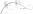
\includegraphics[width=0.8\textwidth]{figs_part2/cosserat_kinematics/cosserat_cross_section.pdf}
        \caption{Illustration of the kinematics degrees of freedom of the Cosserat rod. The black line is the \textit{center-line} $\mathbf{r}=\mathbf{r}(u)$ where $u \in [0,L_0]$ is the \textit{material coordinate} along the length of the rod, where $L_0$ is a positive real number. When specifying constitutive dynamics, $L_0$ often becomes the \textit{rest-length} of the rod. Two cross-sections at $u=u_1$ and $u=u_2$ are shown with the material frame attached $E = (\mathbf{e}_1\ \mathbf{e}_2\ \mathbf{e}_3)$, which are the red, green and blue arrows respectively, of which the latter two are the \textit{directors} of the rod. Note that having two directors, as opposed to a single director normal to the cross-section, allows for a twisting degree of freedom as can be seen in Fig.~\ref{fig:twisting cosserat rod}.}
        \label{fig:Cosserat kinematic degrees of freedom}
\end{figure}

\begin{figure*} 
    \centering
     
    \begin{subfigure}[b]{0.49\textwidth}  
        \centering 
        \includegraphics[width=\textwidth]{figs_part2/cosserat_kinematics/straight.png}
        \caption[Straight Cosserat rod]%
        {{\small Straight Cosserat rod}}    
        \label{fig:straight cosserat rod}
    \end{subfigure}
    \hfill
    \begin{subfigure}[b]{0.49\textwidth}
        \centering
        \includegraphics[width=\textwidth]{figs_part2/cosserat_kinematics/extend.png}
        \caption[Extending Cosserat rod]%
        {{\small Extending Cosserat rod}}    
        \label{fig:extending cosserat rod}
    \end{subfigure}    
    
    \vskip\baselineskip    
    \begin{subfigure}[b]{0.49\textwidth}
        \centering
        \includegraphics[width=\textwidth]{figs_part2/cosserat_kinematics/shear.png}
        \caption[Shearing Cosserat rod]%
        {{\small Shearing Cosserat rod}}    
        \label{fig:shearing cosserat rod}
    \end{subfigure}
    \hfill
    \begin{subfigure}[b]{0.49\textwidth}  
        \centering 
        \includegraphics[width=\textwidth]{figs_part2/cosserat_kinematics/twist.png}
        \caption[Twisting Cosserat rod]%
        {{\small Twisting Cosserat rod}}    
        \label{fig:twisting cosserat rod}
    \end{subfigure}

    \vskip\baselineskip
    \begin{subfigure}[b]{0.49\textwidth}   
        \centering 
        \includegraphics[width=\textwidth]{figs_part2/cosserat_kinematics/bend.png}
        \caption[Bending Cosserat rod]%
        {{\small Bending Cosserat rod}}    
        \label{fig:bending cosserat rod}
    \end{subfigure}
    \hfill
    \begin{subfigure}[b]{0.49\textwidth}   
        \centering 
        \includegraphics[width=\textwidth]{figs_part2/cosserat_kinematics/bend_shear_twist.png}
        \caption[Bending, shearing and twisting Cosserat rod]%
        {{\small Bending, shearing and twisting Cosserat rod}}    
        \label{fig:bending, shearing and twisting cosserat rod}
    \end{subfigure}
    \caption[ The average and standard deviation of critical parameters ]
    {\small Examples of deformations of the Cosserat rod. The transparent gray tubes is the bulk of the Cosserat rod, with the center-line (black line) running through its radial center. The material frame and cross-section are shown at intermittent points along the center-line, along with the surface fibres traced out by the directors $\mathbf{e}_2$ and $\mathbf{e}_3$, green and blue respectively. The tubular radii of the rods depicted were exaggerated in size for illustrative purposes. (a) A straight Cosserat rod suffering no deformation. (b-f) Examples of extension, shearing, twisting and bending deformations.} 
    \label{fig:Examples of Cosserat deformations}
\end{figure*}

A Cosserat rod can be defined as a curve in Euclidean space $\mathbf{r}(u) \in \mathbb{R}^3,\ u \in [0, L_0]$, known as the \textit{center-line} and where $L_0$ is (in a dynamical setting) the \textit{rest-length} of the rod, and an orthogonal triad $E(u) = \begin{pmatrix} \mathbf{e}_1(u) & \mathbf{e}_2(u) & \mathbf{e}_3(u) \end{pmatrix} \in \mathbb{R}^3$. The \textit{material frame} $E(u)$ represents the, in general ellipsoidal, cross-section of the rod at each \textit{material point} $u$ along the center-line. The vectors $\mathbf{e}_2(u)$ and $\mathbf{e}_3(u)$ are the aforementioned directors of the Cosserat rod, which can vary in length and represent the semi-minor and semi-major axes of the cross-section at $u$. The vector $\mathbf{e}_1(u)$ is normal to the cross-section at $u$ and is defined as $\mathbf{e}_1(u) = (\mathbf{e}_2(u) \times \mathbf{e}_3(u)) / |\mathbf{e}_2(u) \times \mathbf{e}_3(u)|$, where $\times$ is the 3-dimensional cross-product and $|\cdot|$ is the standard norm in Euclidean space.

The deformations and rotations of the center-line and material frame comprise the full kinematic degrees of freedom of the Cosserat rod. Often in applications the cross-section is approximated to be of constant shape along the rod, in which case the we restrict the directors to be inextensible and orthogonal, and thus $E(u)$ is then an orthonormal triad. See Fig.~\ref{fig:Cosserat kinematic degrees of freedom} for an illustration of a Cosserat rod with circular cross-section. In the literature this class of Cosserat rod is known as a \textit{special Cosserat rod} \citep{antmanSpecialCosseratTheory1995, rubinCosseratRods2000, altenbachCosseratMedia2013}. Henceforth, unless stated otherwise, by Cosserat rod we mean a special Cosserat rod.

The kinematic degrees of freedom of the rod are thus: smooth translations of the curve $\mathbf{r}$ and smooth rotations the material frame-field $E$. In other words, the center-line can bend, and the cross-section can shear and twist around the center-line and extend tangentially across its length, as is illustrated in Fig.~\ref{fig:Cosserat kinematic degrees of freedom}. The extension of the rod can be captured by the scalar $h(u) = \left| \frac{\partial \mathbf{r}}{\partial u} \right| $, which can be seen as the square root of the metric on the center-line induced by the Euclidean metric on $\mathbb{R}^3$. $h$ relates the material coordinate $u$ to the arc-length coordinate $s$ as
\begin{equation}
ds = h(u) du
\end{equation}
such that $ \left| \frac{\partial \mathbf{r}}{\partial s} \right| = 1$ for all $s \in [0, L]$ where
\begin{equation}
L[h(u)] = \int_0^{L_0} h(u) du
\end{equation}
is the total arc-length of the center-line. Thus any point $u$ for which $h(u)=1$ is not suffering an extension. Shear and twist deformations can be distinguished by noting that the former denotes the orientation $\mathbf{e}_1$ of the cross-section deviating from being parallel to the center-line, whilst the latter denotes rotations of the material frame around $\mathbf{e}_1(u)$. Henceforth we will also distinguish the length elements $ds$ and $du$ as the \textit{length element} and \textit{material length element} respectively.

We now add time to the picture, and consider the motion of the Cosserat rod as the result of arbitrary translational and angular velocity fields. Let the center-line $\mathbf{r}(t,u)$ and the material frame $\mathbf{e}_i(t,u)$ be functions of time, then the temporal evolution of the rod is
\begin{subequations} \label{eq:Cosserat rod kinematic equations}
  \begin{align}
\dot{\mathbf{r}} & = \mathbf{V} \label{eq:Cosserat rod r kinematic eom} \\
\dot{\mathbf{e}}_i & = \boldsymbol{\Omega} \times \mathbf{e}_i \label{eq:Cosserat rod e_i kinematic eom}
  \end{align}
\end{subequations}
from initial boundary conditions at $t=0$, and where $\mathbf{V} = \mathbf{V}(t,u)$ and $\boldsymbol{\Omega} = \boldsymbol{\Omega}(t,u)$ are arbitrary translation and angular velocities.

Dynamical equations of motion for the Cosserat rod are found by imposing balance laws on the momentum and moments of the polar continua. For undirected media, the conservation of mass and linear momentum balance are used to determine the dynamics, given constitutive and body forces. For directed media, in addition to the above, further conservation laws must be imposed to establish the director dynamics.

For a Cosserat rod with mass density $\rho_0^V$ and cross-sectional area $A$ in its reference configuration, the linear momentum of the rod is $\mathbf{P} = \rho^V_0 A \dot{\mathbf{V}}$, as is the case in classical continuum mechanics. We also introduce the director angular momentum $\mathbf{L} = I \boldsymbol{\Omega}$, where $I \in \mathbb{R}^{3 \times 3}$ is a moment of inertia matrix for the cross-section. As will be shown in Sec.~\ref{ch:Cosserat rods}, imposing the conservation of the linear momentum of the rod and the director angular momentum leads, as was first derived in \citep{cosseratTheoryDeformableBodies1909}, to
\begin{subequations} \label{eq:Cosserat rod dynamical equations of motion}
  \begin{align}
\dot{\mathbf{P}} & = \mathbf{F}' + \mathbf{f} \label{eq:Cosserat rod linear momentum balance} \\
\dot{\mathbf{L}} & = \mathbf{M}' + \mathbf{r}' \times \mathbf{F} + \mathbf{m}, \label{eq:Cosserat rod angular momentum balance} \\
\mathbf{F} & = 0,\ \text{at } u=0 \text{ and } u=L_0 \label{eq:Cosserat rod F bc}  \\
\mathbf{M} & = 0,\ \text{at } u=0 \text{ and } u=L_0 \label{eq:Cosserat rod M bc}
  \end{align}
\end{subequations}
where $\mathbf{F}$ are the constitutive forces acting on the rod, $\mathbf{f}$ the body forces per unit material length, $\mathbf{M}$ the constitutive director moments and $\mathbf{m}$ the body moment per unit material length. Eq.~\ref{eq:Cosserat rod linear momentum balance} is in a form familiar to classical continuum mechanics, which can be seen by comparing it to Eq.~\ref{eq:Cauchy momentum equation}, whilst Eq.~\ref{eq:Cosserat rod angular momentum balance} is particular to the setting of directed media. Equation \ref{eq:Cosserat rod dynamical equations of motion} and Eq.~\ref{eq:Cosserat rod kinematic equations} together form a closed set of first-order equations in time and space for the kinematics and dynamics of a Cosserat rod.

We note here that up until this point we have considered an open Cosserat rod where $\mathbf{r}(0,t) \neq \mathbf{r}(L_0,t)$. The dynamics of a closed Cosserat rod, for which the center-line and frame are periodic functions of $u$, are identical with the exception of the omission of the boundary conditions Eq.~\ref{eq:Cosserat rod F bc} and Eq.~\ref{eq:Cosserat rod M bc}.

Equation \ref{eq:Cosserat rod dynamical equations of motion} can be derived directly from the balance laws of classical continuum mechanics, as shown in \citep{parkerDerivationNonlinearRod1984, rubinCosseratRods2000}, under the kinematic assumption that the cross-sections traced out by the directors correspond to the bulk of a three-dimensional tube of undirected point-continua. For illustrative purposes this kinematic assumption deserves further elaboration. In precise mathematical language, let $M \subset \mathbb{E}$ and let $\mathbf{x} : D \to M$ be the \textit{material coordinate} function from the domain
\begin{equation}
D = \{ (X_1, X_2, X_3)\ :\ X_1^2 + X_2^2 = R^2\ \text{and}\ X_3 \in [0,L_0]  \}
\end{equation}
where $R$ is a given fixed tubular radius of the Cosserat rod. Given a Cosserat rod configuration $(\mathbf{r},\ E)$, we define $M$ via the material coordinate function as
\begin{equation}
\mathbf{x}(\mathbf{X}) = \mathbf{r}(X_3) + X_j \mathbf{e}_j,\ j=2,3
\end{equation}
such that $M$ is the image of $\mathbf{x}$. Here the material coordinate $X_3$ corresponds to the coordinate $u$. We see how the Cosserat rod can be viewed as the result of a coarse-graining procedure from the full three-dimensional continuum setting, replacing the cross section at each $u$ with two directors, thus reducing the spatial coordinates of the system from three to one.

We now conclude this section by making some remarks, prefacing the discussions in subsequent chapters, on the geometric properties of the Cosserat rod. The kinematic equations of motion Eq.~\ref{eq:Cosserat rod r kinematic eom} and Eq.~\ref{eq:Cosserat rod e_i kinematic eom} shows explicitly that the rod moves according to infinitesimal translations $\mathbf{V}dt$ and rotations $\boldsymbol{\Omega} \times \mathbf{e}_i$ respectively. This entails that we can identify the kinematic structure of the Cosserat rod with the \textit{Lie group} of Euclidean transformations of translations and rotations $SE(3)$ \citep{simoGeometricallyexactRodModel1991, simoThreedimensionalFinitestrainRod1986}. In particular the rod itself can be parametrised in terms of sub-manifolds of $SE(3)$ and, as will be the main subject of Sec.~\ref{ch:Cosserat rods}, from which geometricised kinematic and dynamical equations of motion can be derived programmatically. In the following section some mathematical foundations will be introduced, necessary for the subsequent chapters of this part of the thesis.

{\color{red} I think this should reference some more beneficial properties of using Lie group, like the lack of coordinitisation and some rerefernec to parameterising using the Lie algebra / differential invariants. But I can add that later when I've written the subsequent mathematical subsections. }

% Note that these equations accurately remain invariant under rigid body transformation (just make sure to look up the significance of this again).

{\color{red} Should also introduce Cosserat sheet, althouhg can do that later after you've derived the equations of motion etc.}

% In the purely mechanical three-dimensional theory the balance of angular momentum places restrictions on the constitutive equations which require the Cauchy stress tensor to be symmetric. Also, the conservation of mass and the balance of linear momentum are used to determine the mass density and the position of each material point in the continuum. For the Cosserat theories that will be developed in the next chapters, alternative equations representing the conservation of mass and the balances of linear and angular momentum will be used in a similar manner to determine the mass density and the position of each material point. However, the Cosserat theories will introduce additional kinematical quantities called director vectors at each material point which also need to be determined by additional balance laws. In order to motivate the forms for these balance laws, it is convenient to consider an averaged form of the balance of linear momentum

% The global forms of the balance laws of the Cosserat theory of shells are similar to those of the three-dimensional theory in the sense that they include the notions of conservation of mass and balances of linear and angular momentum. Moreover, these equations are used to determine the current values of a mass density p and the position vector x of points on the surface 5 of the shell. Also, the balance of angular momentum places restrictions on the constitutive equations of the shell theory that are similar in nature to the restrictions (3.2.32) associated with the three-dimensional theory. However, in contrast with the three-dimensional theory, the Cosserat theory of shells introduces the additional kinematic quantity d3 at each point of the surface 5 of the shell which also must be determined by a balance law. Consequently, the Cosserat theory of shells requires an additional balance law called the balance of director momentum.

% In this section it will be shown that the balance laws of the Cosserat theory can be developed by using the kinematic assumption (4.2.7) and the balance laws of the threedimensional theory.



%- Define the polar continua precisely that we are interested in: Cosserat rod with orthonormal directors. Figures:
%  - One figure (perhaps just in Inkscape, like the one you've made earlier) that just shows the cross section.
%  - Show the twisting, bending and shearing degrees of freedom. These should be 3D. In Mathematica you should write code that can take in cosserat data and spit out a 3D model figure.
%- Introduce the kinematic and dynamics equations of motion, in terms of $\mathbf{r}$ and $\mathbf{e}_i$. 
%- Note that these equations accurately remain invariant under rigid body transformation (just make sure to look up %the significance of this again).
%- Note that the equations move according to Euclidean transformation, motivates the subsequent sections.

\section{Mathematical preliminaries}

As will be further discussed in Ch.~\ref{ch:Cosserat rods}, directed media can be seen as either sub-manifolds of \textit{homogeneous spaces} or sub-manifolds of \textit{Lie groups}. Through this lens, a fully geometricised and non-coordinate form of the equations of motion of such systems can be derived. This section serves primarily to establish establish the mathematical foundation and rigour of the programme, and therefore has a level of mathematical abstraction higher than that of the subsequent chapters. The reader not interested in these details may proceed to Ch.~\ref{ch:Cosserat rods}, and return to this section intermittently to fill gaps in notation and conceptual knowledge.

For a fuller treatment of the concepts introduced in this section the reader can consult the following references for further exposition \citep{clellandFrenetCartanMethod2017, kleinDevelopmentMathematics19th1979, marsdenIntroductionMechanicsSymmetry2013, marleHenriPoincareNote2013a}.

\subsection{Differential geometry}

Pullbacks and pushforwards

Define the Lie bracket in component form

\begin{equation} \label{eq:lie bracket in component form}
[X, Y] = (X^j \partial_j Y^i - Y^j \partial_j X^i) \partial_i
\end{equation}

\subsection{Exterior calculus}

In calculus, the differential of a scalar function $f : \mathbb{R}^3 \to \mathbb{R}$ is often written as
\begin{equation}
df = \frac{\partial f}{\partial x} d x + \frac{\partial f}{\partial y} d y + \frac{\partial f}{\partial z} d z.
\end{equation}
This can be generalised for differentiable manifolds. Let $M$ be a smooth $d$-dimensional manifold, $p \in M$ a point on the manifold, $X \in \Gamma(TM)$ a vector field on $M$ and $f \in C^\infty(M)$ be a smooth function on $M$. We define the map $df : TM \to \mathbb{R}$ as
\begin{equation} \label{eq:df action}
(df(X))(p) = X_p(f).
\end{equation}
Here $df$ is an example of a \textit{scalar-valued $1$-form}. Analogously, scalar functions $f \in C^\infty(M)$ are known as \textit{scalar-valued $0$-forms}. Scalar-valued $p$-form are linear maps $\prod_{i=1}^p TM \to \mathbb{R}$, where $\prod$ signifies the repeated Cartesian product. The operator $d$ is the \textit{exterior derivative}, which in general maps $p$-forms to $(p+1)$-forms. Any $(p+1)$-form that can be written as the exterior derivative of a $p$-form is referred to as \textit{exact}. Conversely, any $p$-form $\phi$ that satisfies $d \phi = 0$ is \textit{closed}. Locally, closed $p$-forms are always exact, which is known as the \textit{Poincaré lemma}. 
 
Let $x^i : U \to \mathbb{R},\ i=1,\dots,d$ be coordinate functions for some neighbourhood $U \subset M$. Then $df$ can then be locally expressed in in $U$ as
\begin{equation} \label{eq:df expansion}
df = \frac{\partial f}{\partial x_i} d x^i
\end{equation}
such that $df(X) = \frac{\partial f}{\partial x^i} dx^i(X) = \frac{\partial f}{\partial x^i} X^i$, where $X \in \Gamma(TM)$. Not all $1$-forms are closed, and can thus not be written in the form of Eq.~\ref{eq:df expansion}, but they can always be expanded in a coordinate basis as $\phi = a_i dx^i$, where $a_i \in C^\infty(M),\ i=1,\dots,d$ are the coefficients of $\phi$ in this basis.

The \textit{symmetric product} of a $p$-form $x$ and $q$-form $y$ is written as $x \otimes y$. For $p=q=1$, we have
\begin{equation}
(x \otimes y)(X, Y) = \phi(X) \psi(Y)
\end{equation} 
where $X, Y \in \Gamma(TM)$ are two vector fields. For a general $1$-form, its exterior derivative can be expressed locally as
\begin{equation} \label{eq:exterior derivative of 1-form}
d\phi = d a_i \wedge dx^i.
\end{equation}
where $\wedge$ is the \textit{wedge product}. Let $x$ and $y$ be a $p$-form
and a $q$-form respectively, then $x \wedge y$ is a $(p+q)$-form defined as
\begin{equation}
x \wedge y = x \otimes y - y \otimes x
\end{equation}
and satisfies
\begin{equation}
y\wedge x=(-1)^{pq}x\wedge y.
\end{equation}
and
\begin{equation} \label{eq:exterior derivative of wedge product}
d(x \wedge y) = dx \wedge y + (-1)^p x \wedge d y.
\end{equation}
The wedge product of a sequence of forms can be written as
\begin{equation}
\bigwedge_{i=1}^n z^i = dz^1 \wedge dz^2 \wedge \dots \wedge dz^n
\end{equation}
where each $z^i$ is a $p^i$-form. Due to the anti-symmetry of the wedge products of $1$-forms, we have
that $df \wedge df = 0$ for any $f \in C^\infty(M)$. If $x$ and $y$ are two $1$-forms, then the product $x \wedge y$ is a mapping $TM \times TM \to \mathbb{R}$, and can be evaluated on two vector fields $X,Y \in \Gamma(M)$ as
\begin{equation}
(x \wedge y)(X, Y) = x(X) y(Y) - x(Y) y(X).
\end{equation}

We will now derive a coordinate-free expression for the exterior derivative of a $1$-form. Let $\phi = a_i dx^i$, then
\begin{equation} \label{eq:exterior derivative of 1-form evaluated}
\begin{aligned}
d\phi(X,Y) & = da_i(X) Y^i - da_i(Y) X^i \\
 & = \frac{\partial a_i}{\partial x^k} X^k Y^i - \frac{\partial a_i}{\partial x^k} Y^k X^i \\
 & =  \left( X^k \frac{\partial}{\partial x^k} ( a_i Y^i) - a_i X^k \frac{\partial Y^i}{\partial x_k} \right) -  \left( Y^k \frac{\partial}{\partial x^k} ( a_i X^i) - a_i Y^k \frac{\partial X^i}{\partial x_k} \right) \\
 & = X^k \frac{\partial}{\partial x^k} ( a_i Y^i) - Y^k \frac{\partial}{\partial x^k} ( a_i X^i) - a_i  \left( X^k \frac{\partial Y^i}{\partial x_k} - Y^k \frac{\partial X^i}{\partial x_k} \right) \\
 & = X(\phi(Y)) - Y(\phi(X)) - \phi([X,Y])
\end{aligned}
\end{equation}
where we used Eq.~\ref{eq:lie bracket in component form}.

Intuitively, a $1$-form can be seen as measuring an infinitesimal oriented length. A $2$-form can be seen as measuring an infinitesimal oriented area. A $p$-form measures an infinitesimal oriented $p$-dimensional volume. There is therefore a natural notion of integrals of $p$-forms. In general, a $p$-form $\phi$ defined on a manifold $M$ can be integrated on a $p$-dimensional sub-manifold of $M$.

If $M$ is $d$-dimensional, then the integration of $d$-forms and $1$-forms coincides with the usual notion of integration in multi-variate calculus. Let $U \subset M$ with coordinates $x^i : U \to \mathbb{R}^d$, and let $\gamma \subset U$ be a $1$-dimensional sub-manifold of $U$, and let $\phi = h_i dx^i$ be a general $1$-form and $\psi = g \bigwedge_{i=1}^d dx^i$ a general $d$-form then
\begin{subequations}
\begin{align}
\int_\gamma \phi & = \int_\gamma h_i d x^i \\
\int_U \psi & = \int_U g \bigwedge_{i=1}^d dx^i = \int_U g\ dx^1 dx^2 \dots dx^d
\end{align}
\end{subequations}
where the right-most term in the equalities are the standard multi-variate integrals. For a $d$-dimensional manifold, a $d$-form like $\psi$ is called a \textit{volume form}. If $V \subset M$ is a $(p-1)$-dimensional sub-manifold and $\phi$ is a $p$-form, then it can be shown that
\begin{equation} \label{eq:stokes theorem}
\int_V d \phi = \int_{\partial V} \phi
\end{equation}
where $\partial V$ signifies the boundary of $V$. Eq.~\ref{eq:stokes theorem} is called \textit{Stokes' theorem}.

Consider a $1$-form expressed locally as $\phi = a_i dx^i$. Under change of coordinates, it transforms as
\begin{equation} \label{eq:dx transform}
a_i dx^i = a_i \frac{\partial x^i}{\partial \tilde{x}^i} d\tilde{x}^i.
\end{equation}
From Eq.~\ref{eq:dx transform}, it can be shown that $d$-forms transform as
\begin{equation}
f \bigwedge_{i=1}^d dx^i = \left( \text{det} \left[ \frac{\partial \mathbf{x} }{ \partial \tilde{\mathbf{x}} } \right] f \right) \bigwedge_{i=1}^d d\tilde{x}^i
\end{equation}
where $\frac{\partial \mathbf{x} }{ \partial \tilde{\mathbf{x}} }$ is the Jacobian matrix of the coordinate transformation.

\subsection{Lie groups}

\begin{definition}
A $d$-dimensional \textit{Lie group} is a set $G$ that is both a group and a differentiable manifold of dimensions $d$, where the multiplication map $G\times G \to G$
\begin{equation}
(g,h) \mapsto gh \in G
\end{equation}
and inverse $G \to G$
\begin{equation}
g \mapsto g^{-1}
\end{equation}
are smooth maps.
\end{definition}

For all Lie groups under our consideration, $G$ can be represented as sub-manifold of $GL(n)$ under a map, the group of $n\times n$ invertible matrices for some $n \geq d$, under the map $g : G \to \subset GL(n)$. We call the image of this map $\tilde{G}$, which is the set of invertible matrices in $GL(n)$ that forms a representation of $G$. Henceforth, unless stated to be otherwise explicitly, we will use the short-hand $g \in G$ instead of $g \in \tilde{G}$, thus essentially identifying the matrix Lie group representation with the Lie group itself.

For each element $g \in G$, the \textit{left multiplication} map $L_g : G \to G$ is defined as $L_g h = gh$ where $h \in G$. Similarly, the \textit{right multiplication} map $R_g : G \to G$ is defined as $R_g h = hg$. For maps between smooth manifolds $\Psi : M \to N$, we define its \textit{derivative} at $p \in M$ as the mapping $D\Psi_p : T_p M \to T_{\Phi(p)} N$ given by the formula
\begin{equation} \label{eq:derivative of linear map}
D\Psi_p (v)(f) = v(f \circ \Psi)
\end{equation}
for $v \in T_p M$ and $f \in C^\infty(N)$. In particular, the derivative of the left multiplication at $h\in G$ is a mapping $(DL_g)_h : T_hG \to T_{gh} G$, which can be shown to be equal to
\begin{equation}
(DL_g)_h(X) = gX
\end{equation}
where $X \in T_h G$. For any Lie group $G$ there is an associated \textit{Lie algebra} $\mathfrak{g}$, which is the tangent space $T_e G$ at the identity, where $e \in G$ is the identity element. $\mathfrak{g}$ is thus a vector space of the same dimension $d$ as $G$. For any vector $V \in \mathfrak{g}$, we can define a \textit{left-invariant vector field} $\tilde{V}$ defined on each $g \in G$ as
\begin{equation} \label{eq:left-invariant vector field}
\tilde{V}_g = (DL_g)_e (V).
\end{equation}
Now let $E_i,\ i=1,\dots,d$ be a basis for $\mathfrak{g}$, then it can be shown that the corresponding left-invariant vector-fields $\tilde{E}_i$ form a global basis for the tangent bundle $TG$. This implies that the tangent bundle of Lie groups $G$ are isomorphic to the Cartesian product $TG \cong G \times \mathfrak{g}$. Furthermore, it is notable that the global basis is constructed without specifying coordinate functions on the manifold.

The \textit{expontential map} $\exp : \mathfrak{g} \to G$ relates Lie algebra elements to corresponding Lie group elements, and for matrix Lie groups this is explicitly given by the matrix exponential. Intuitively this mapping can be understood by considering the curve $\gamma(t) = \exp ( t V ) \in G$, where $V \in \mathfrak{g}$. Differentiating the curve gives us
\begin{equation}
\begin{aligned}
\frac{d}{dt} \gamma(t) & = \exp (t V) V \\
& = (D L_{ \exp (t V) } )_e (V) = \tilde{V}_g
\end{aligned}
\end{equation}
The curve $\gamma$ is thus a flow-line of the left-invariant vector field $\tilde{V}$.

The Lie algebra $\mathfrak{g}$ also has a product structure known as the \textit{Lie bracket} $[\cdot, \cdot] : \mathfrak{g} \times \mathfrak{g} \to \mathfrak{g}$ given by
\begin{equation}
[X, Y] = XY - YX
\end{equation}
for $X,Y \in \mathfrak{g}$. To see its relation to the Lie group, we introduce the \textit{adjoint action} of a Lie group on its Lie algebra  $\text{Ad} : G \times \mathfrak{g} \to \mathfrak{g}$ given by
\begin{equation}
\text{Ad}_g Y = g Y g^{-1}
\end{equation}
for each $g\in G$, $\text{Ad}_g$ is thus an automorphism of the Lie algebra. Let $g(t) = \exp(t X)$, with Taylor expansion $g(t) = I + t X + O(t^2)$. The the infinitesimal action of the automorphism $\text{Ad}_g$ can then be found by expanding it as
\begin{equation}
\text{Ad}_g Y = Y + t[X, Y] + O(t^2).
\end{equation}
This motivates the definition of the adjoint action of the Lie algebra \textit{on itself} $\text{ad} : \mathfrak{g} \times \mathfrak{g} \to \mathfrak{g}$ given by
\begin{equation}
\text{ad}_X Y = [X, Y].
\end{equation}
Let $E_a,\ a=1,\dots,d$ be a basis for Lie algebra $\mathfrak{g}$, then the Lie bracket can also be written in terms of its \textit{structure constants} $f^a_{bc} \in \mathbb{R}$
\begin{equation}
[E_a, E_b] = f_{ab}^c E_c, \quad a,b,c=1,\dots,d.
\end{equation}
The Lie algebra can be \textit{defined} as a vector space $\mathfrak{g}$ equipped with Lie bracket, where the latter is fully specified by the structure constants. If $G$ is connected, then $G$ is exactly equal to the image of $\mathfrak{g}$ under the exponential map \footnote{If $G$ is not connected, $\exp(\mathfrak{g})$ is equal to the sub-group of $G$ that is connected to the identity element $e \in G$.}. This is known as the \textit{Lie algebra-Lie group correspondence}. We thus see that the structure constants encapsulates the full geometry of the Lie group.

For a $d$-dimensional Lie group $G$, with Lie algebra $\mathfrak{g}$, a linear map $\prod_{i=1}^p TG \to \mathfrak{g}$ is a \textit{Lie algebra-valued} $p$-form. A general Lie algebra-valued $1$-form $X : TG \to \mathfrak{g}$ can be written as
\begin{equation}
X = a_i^a E_a dx^i
\end{equation}
where $E_a,\ a=1,\dots,d$ is a basis for $\mathfrak{g}$, $x^i \in C^\infty(G),\ i=1,\dots,d$ are global coordinate functions on $G$, and $a_i^a \in C^\infty(G),\ i,a=1,\dots,d$ are the coefficients of $X$ in this basis. The exterior derivative of a Lie-algebra valued form can be computed by simply applying it directly on the scalars in the expression. For example, the exterior derivative of a Lie algebra-valued $1$-form is
\begin{equation}
dX = E_a\ d(a_i^a dx^i).
\end{equation}
Similarly, let $Y = b_i^a E_a dx^i$, then the wedge product of two $1$-forms can be computed as
\begin{equation}
X \wedge Y = E_a E_b a_i^a b_j^b\ dx^i \wedge dx^j
\end{equation}
where $E_a E_b$ denotes ordinary matrix multiplication. Note that the wedge product of two Lie algebra-valued forms is not necessarily Lie algebra-valued.

The following are some examples of Lie groups:
\begin{itemize}
\item The positive real numbers $\mathbb{R}^+$ equipped with multiplication forms an \textit{abelian} Lie group, where all elements commute with each other.

\item The orthogonal group $O(n)$ which is the space of orthogonal $n \times n$ matrices. Its Lie algebra $\mathfrak{o}(n)$ comprises the space of anti-symmetric $n \times n$ matrices.

\item The special orthogonal group $SO(n)$ is the set of matrices $R \in SO(n)$ for which $\det{R} = 1$. Its Lie algebra $\mathfrak{so}(n)$ is equal to $\mathfrak{o}(n)$.

\item The translation group $T(n)$ is the group of translations in $n$-dimensional Euclidean space.

\item The special Euclidean group $SE(n)$ is the group of translations and rotations in $n$-dimensional space, and can be written as the semi-direct product $SE(n) = T(n) \rtimes SO(n)$.
\end{itemize}

%As a motivating example, consider the general Lagrangian for a closed system of $N$ pair-wise interacting point particles
%\begin{equation}
%\begin{aligned}
%L & = K - U \\
%K & = \sum_i m_i |\dot{\mathbf{x}}_i|^2 \\
%U & = \sum_{i,j < i} U_{ij}(|\mathbf{x}_i - \mathbf{x}_j|) 
%\end{aligned}
%\end{equation}
%where $K$ and $U$ is the total kinetic and potential energy of the system respectively, and $U_{ij}$ is the interaction potential between the $i$th and the $j$th particle. 

%It is also possible to generate permissible forms of the Lagrangians of classical mechanics by \textit{imposing} Galilean invariance. \citep{landauMechanicsVolume1982}

%We say that $L$ is $G$-invariant if the resulting equations of motions are invariant under the transitive action of $G$.

\subsection{Homogeneous spaces}

List all the main homogeneous spaces found in
%https://en.wikipedia.org/wiki/Homogeneous_space#Formal_definition

Introduce principal bundles.

Define transitive action. Define homogeneous space both as a quotient $G/H$ but also as a topological space where a group $G$ acts transitively.

Introduce Euclidean space $\mathbb{E}^d$, as the vector space $\mathbb{R}^d$ equipped with an inner product.

\subsection{The Maurer-Cartan form} \label{sec:The Maurer-Cartan form}

We have seen that the Lie group $G$ can be fully reconstructed using the structure constants $f_{ab}^c$ of its Lie algebra $\mathfrak{g}$. The same geometric information is also contained in its left-invariant vector fields Eq.~\ref{eq:left-invariant vector field}\footnote{Equivalently, the right-invariant vector fields contains the same information.}, which can be encapsulated using a Lie algebra-valued $1$-form called the \textit{Maurer-Cartan form} $\omega : TG \to \mathfrak{g}$, which is defined as
\begin{equation} \label{eq:Maurer-Cartan form}
\omega(v) = (DL_{g^{-1}})_g (v)
\end{equation}
for any $v \in T_g G$. The Maurer-Cartan form thus maps the tangent spaces at any point $g$ to the tangent space at the identity $\mathfrak{g}$.

Let $X, Y \in \mathfrak{g}$ and let $v_X = (DL_g)_e(X)$ and $v_Y = (DL_g)_e(Y)$ be their corresponding left-invariant vector fields. Then the Maurer-Cartan form satisfies
\begin{equation} \label{eq:recovering the Lie algebra from MC form}
\omega([v_X, v_Y]) = [X, Y]
\end{equation}
where the argument of $\omega$ on the left-hand side is the Lie bracket of vector fields. Eq.~\ref{eq:recovering the Lie algebra from MC form} can be derived by noting that for any diffeomorphism $\Psi : M \to N$, we have that $D\Psi([v,w]) = [D\Psi(v), D\Psi(w)]$ where $v,w \in \Gamma(TM)$. By recovering the Lie bracket of the Lie algebra from the Maurer-Cartan form, we thus see that it encapsulates all geometric information about the Lie group.

From Eq.~\ref{eq:exterior derivative of 1-form evaluated} we have that
\begin{equation}
d \omega(v,w) = v(\omega(w)) - w(\omega(v)) - \omega([v,w]).
\end{equation}
If $v$ and $w$ are left-invariant, then $v(\omega(w)) = w(\omega(v)) = 0$, and we get
\begin{equation} \label{eq:mauer-cartan equation invariant form}
d \omega(v,w) + \omega([v,w]) = 0
\end{equation}
but as left-invariant vectors span the whole tangent bundle, this equation must also hold for arbitrary for all vector fields. Eq.~\ref{eq:mauer-cartan equation invariant form} is known as the \textit{Maurer-Cartan equation}, and can be seen as the defining equation for $\omega$, and will be instrumental in future chapters.

For the applications in the coming chapters, it is more convenient to work in a matrix representation of the Maurer-Cartan form, given by
\begin{equation} \label{eq:Maurer-Cartan form as matrix}
\omega = g^{-1} dg.
\end{equation}
To explain the above expression, we temporarily reintroduce the distinction between abstract Lie group elements $x \in G$, and their matrix representations $g(x) \in \tilde{G}$. Eq.~\ref{eq:Maurer-Cartan form as matrix} is more accurately written as $\omega_x = g(x)^{-1} Dg_x$ where $x \in G$ is here an abstract (non-matrix) Lie group element. To see the correspondence between Eq.~\ref{eq:Maurer-Cartan form} and Eq.~\ref{eq:Maurer-Cartan form as matrix}, we first note that the derivatives of linear maps $\Psi : M \to N$, defined in Eq.~\ref{eq:derivative of linear map}, is equivalent to the exterior derivative of a $0$-form. Thus $dg = Dg$, and $dg_x : T_x G \to T_{g(x)} \tilde{G}$, which is computed as a matrix of $1$-forms. Finally we then left-translate $dg$ to get $g^{-1} dg : TG \to \mathfrak{g}$.

Finally, we derive Eq.~\ref{eq:mauer-cartan equation invariant form} in matrix form. We take the exterior derivative of Eq.~\ref{eq:Maurer-Cartan form as matrix}
\begin{equation} \label{eq:Mauer-Cartan equation in matrix form}
\begin{aligned}
d \omega & = d(g^{-1} dg) \\
& = - (g^{-1} dg g^{-1}) \wedge dg + g^{-1} d^2 g \\
& = - \omega g^{-1} \wedge dg,
\end{aligned}
\end{equation}
to get
\begin{equation}
d \omega + \omega \wedge \omega = 0
\end{equation}
where we have used the fact that $dg$ is a matrix of closed $1$-forms, so that $d^2 g=0$, that the wedge product commutes with matrix multiplication, and $d(g^{-1} g) = 0$ to find an expression for $d g^{-1}$.

\subsection{Sub-manifolds of homogeneous spaces} \label{sec:Sub-manifolds of homogeneous spaces}

The exposition in this section follows closely that of \citep{clellandFrenetCartanMethod2017}. The Maurer-Cartan form and the Maurer-Cartan equation are particularly useful when studying sub-manifolds of homogeneous spaces. If $M \subset G/H$, let $\Phi : W \to M$ be a differentiable map, where $W$ is some $n$-dimensional manifold, where $\mathbb{T}^n$ is the $n$-dimensional torus, for some $n$. The \textit{pullback bundle} $\Phi^*G$ of the principal bundle $\pi : G \to G/H$ is defined as
\begin{equation} \label{eq:pullback bundle}
\Phi^*G = \left\{ (u,g) \in W \times G\ :\ \Phi(u) = \pi(g) \right\},
\end{equation}
i.e.~$\Phi^* G$ is a principal bundle over $W$, such that its fibre over $u \in W$ is equal to the fibre of $G$ over $\Phi(u) \in G/H$. $\Phi^* G$ has the map $\hat{\Phi} : \Phi^*G \to G$
\begin{equation}
\hat{\Phi}(u, g) = g
\end{equation}
A \textit{lifting} $\tilde{\Phi} : W \to G$ is a map that satisfies
\begin{equation}
(\pi \circ \tilde{\Phi})(u) = \Phi(u),\ \forall u \in W.
\end{equation}
In subsequent chapters, $\Phi$ will be identified with the space-time kinematic configuration of a system, and the lifting $\tilde{\Phi}$ a $G$-valued field on $W$ that reconstructs $\Phi$. The homogeneous space $G/H$ is then the kinematic configuration space of the system, and $W = (\text{time domain}) \times (\text{material domain})$ will be referred to as the \textit{kinematic base space}. To make this analogy explicit, consider a Cosserat rod with material coordinate $u \in [0, L_0]$ and temporal coordinate $t \in [0, T]$, then $W = [0, T] \times [0, L_0]$ and $\Phi(t,u)$ is the ($G/H$-valued) configuration of the material point $u$ at time $t$. The manifolds $[0, L_0]$ and $[0, T]$ will be called the \textit{material base space} and the \textit{time domain} respectively.

Similarly to how the Maurer-Cartan form can be shown to contain the geometrical information of a Lie group $G$, we will now also show that it can play a similar role for $\Phi$. Let $\tilde{\Phi} : W \to G$ be a differentiable map and let $\xi := \tilde{\Phi}^* \omega$ be the pull-back of the Maurer-Cartan form onto $W$. As $\omega : TG \to \mathfrak{g}$, we have that $\xi : TW \to \mathfrak{g}$. To derive the matrix expression for $\xi$ we note that for any $v \in T_u W$ and $u \in W$ we have
\begin{equation}
\begin{aligned}
\xi(v) & = \tilde{\Phi}^* \omega(v)  = \omega(D\tilde{\Phi}(v)) = ( D L_{ \tilde{\Phi}(u)^{-1} } )_{ \tilde{\Phi}(u) }( D\tilde{\Phi}(v)  ) \\
& = \tilde{\Phi}(u)^{-1} (D\tilde{\Phi})_u (v)
\end{aligned}
\end{equation}
where the definition of the Maurer-Cartan form Eq.~\ref{eq:Maurer-Cartan form}. We can thus write
\begin{equation} \label{eq:pullback Maurer-Cartan}
\begin{aligned}
\xi & = \tilde{\Phi}^{-1} d \tilde{\Phi} \\
& = g^{-1} dg, & g \in \tilde{\Phi}(W)
\end{aligned}
\end{equation}
where used $D\tilde{\Phi} = d\tilde{\Phi}$. The following lemma will show that all information in $\Phi$ is encapsulated by $\xi$, up to global transformations $g \in G$.

\begin{lemma}
Let $W$ be an $n$-dimensional differentiable manifold, and let $\tilde{\Phi}_1, \tilde{\Phi}_2 : W \to G$ be two differentiable maps, and $\xi_i = \tilde{\Phi}^*_i \omega,\ i=1,2$. Then there exists a $g \in G$ such that
\begin{equation} \label{eq:global transformations of Phi}
\tilde{\Phi}_1(u) =  g \tilde{\Phi}_2(u), \quad \forall u\in U
\end{equation}
if and only if $\xi_1 = \xi_2$ where $\omega$ is the Maurer-Cartan form of $G$.
\end{lemma}

\begin{proof}
The following is a reproduction of results in \citep{clellandFrenetCartanMethod2017}, but where we have relaxed the condition that $\text{dim}(W) = n \leq \text{dim}(G/H)$, to allow for arbitrary $n$. There exists a function $f : W \to G$ such that
\begin{equation}
\tilde{\Phi}_1(u) =  f(u) \tilde{\Phi}_2(u), \quad \forall u\in W.
\end{equation}
Differentiating the above, we get
\begin{equation}
d\tilde{\Phi}_1 = df \tilde{\Phi}_2 + f d \tilde{\Phi}_2
\end{equation}
Thus we have
\begin{equation}
\begin{aligned}
\xi_1 = \tilde{\Phi}_1^* \omega & = \tilde{\Phi}_1^{-1} d \tilde{\Phi}_1 \\
& = \tilde{\Phi}_1^{-1} ( df \tilde{\Phi}_2 + f d \tilde{\Phi}_2 ) \\
& = \tilde{\Phi}_1^{-1} df \tilde{\Phi}_2  + \tilde{\Phi}_1^{-1} f \tilde{\Phi}_2 \tilde{\Phi}_2^{-1}  d \tilde{\Phi}_2 \\
& = \tilde{\Phi}_1^{-1} df \tilde{\Phi}_2  + \xi_2,
\end{aligned}
\end{equation}
from which it follows that $\xi_1 = \xi_2$ if and only if $df = 0$.
\end{proof}

The same steps taken to derive Eq.~\ref{eq:Mauer-Cartan equation in matrix form} can be repeated to find that $\xi$ satisfies
\begin{equation} \label{eq:pullback Maurer-Cartan equation}
d \xi + \xi \wedge \xi = 0.
\end{equation}
which are in this context also sometime referred to as the Maurer-Cartan equations. More precisely, they can be seen as the pull-back of the Maurer-Cartan equations on to $W$. The above lemma, along with Eq.~\ref{eq:pullback Maurer-Cartan equation}, are the corner-stones of the general kinematic theory of directed continuum materials, whose kinematic configuration space is a Lie group or homogeneous space, which we will develop in the subsequent chapters. It tells us that \textit{all geometric information in $\Phi$ is encoded in $\xi$}, subject to global transformations Eq.~\ref{eq:global transformations of Phi}, and furthermore that $\xi$ is invariant under said transformations.

In Cartan's \textit{theory of moving frames}, the Maurer-Cartan form is utilised to establish the equivalence of sub-manifolds of homogeneous spaces \citep{levyReviewElieCartan1935, clellandFrenetCartanMethod2017, olverSurveyMovingFrames2005, gardnerMethodEquivalenceIts1989}. For a given homogeneous space $G/H$, $d$-dimensional sub-manifolds can be characterised by a set of \textit{differential invariants}, which are scalar functions defined on the sub-manifold. These differential invariants capture the intrinsic geometry of the sub-manifold, and are invariant under transformations in $H$.  For example, space-curves $\gamma : [0,1] \to \mathbb{R}^3$ can be seen as sub-manifolds the homogeneous space $SE(3) / SO(3) \cong \mathbb{R}^3$. Any such curve is uniquely determined, up to global rigid-body rotations in $SO(3)$, by its \textit{torsion} $\tau(u)$ and \textit{curvature} $\kappa(u)$, where $u \in [0,1]$. The equations that recover $\gamma$ from the two scalar differential invariants are the celebrated \textit{Frenet-Serret} equations. In the language of physics, such a space curve is called a \textit{filament}, and will be treated in Ch.~\ref{ch:Cosserat rods}.

However, the relevance of the above results go beyond being a mathematical nicety. In simulations, working directly with Lie group-valued objects like $\Phi$ can be impractical. As all Lie groups $G$ will in practice be represented as a sub-Lie group of $GL(n)$, numerical errors will in general take values in the space of $n$-by-$n$ matrices. Let $h \in \mathbb{R}^{n \times n}$ represent the error accrued in a single time-step, and let $g \in G$ represent the current state of a simulation. Then it is clear that $g + h \not\in G$. This is inherently due to the non-linearity of the space $G$. In the later chapters, we will instead use the Mauer-Cartan form to formulate the kinematics and dynamics of sub-manifolds of $G$ in terms of its Lie algebra $\mathfrak{g}$. The state of the system thus take values in a linear space, as do the errors, which ensures that in simulations the system never falls out of the correct space.


\begin{comment}
{\color{red} Note to self: In the lemma, by specifying that $U$ has to be open, I'm disqualifying things like $U = S^2$. In which case I do not allow for closed surfaces. It's not clear to me yet whether the above applies to such scenarios yet. I suspect that it does not, and that something extra has to be done with the exterior derivative $d$ on the pullback bundle $\Phi^* G$ (which is no longer flat).

For non-flat manifolds, there's no natural notion of an exterior derivative, but one can be constructed out of the connection. Now the Lie group comes with a connection, in the form of the MC form, and so will induce one on the pullback bundle on $\Phi^* G$, from which an exterior derivative can be constructed. Alternatively, and perhaps more rigorously, we'd have "pull-back" the exterior derivative $d$ onto the pullback bundle.

I think the lemma might actually still hold when $U = S^2$, the issue is Eq.~\ref{eq:pullback Maurer-Cartan equation}. I think what has to be done is to compute the form of $d \xi$ in its invariant formulation (like for Eq.~\ref{eq:mauer-cartan equation invariant form}), but with an exterior derivative on a non-flat manifold.

It could also be the case that this is all fine. I'm starting to suspect that the pullback bundle actually is flat, due to the fact that it is still a cartesian product $U \times G$. See \textit{"This definition also applies when $V$ is considered "outside" the manifold, as you seem to assume. This case is equivalent to saying that the $V_P$ form a trivial vector bundle over the manifold, and therefore they automatically have a flat affine connection, and their covariant derivative reduces to the usual one described in @levap's answer."} from \href{https://math.stackexchange.com/questions/2026904/can-the-formula-for-the-exterior-derivative-be-extended-to-vector-valued-differe}{this} link. Could it be that $\Phi^* G$ is a \href{https://en.wikipedia.org/wiki/Flat_vector_bundle}{flat vector bundle}? Now that I think of it, the "material space-time manifold" $U$ does not necessarily have a connection does it? or at least it doesn't require one.
}
\end{comment}

We have considered a map $\Phi$ and showed its relation to the pullback of the Maurer-Cartan form $\xi$. In applications we will most often have some $\xi : TW \to \mathfrak{g}$ and then reconstruct its corresponding $\Phi$. From Eq.~\ref{eq:pullback Maurer-Cartan}, we have
\begin{equation}
d\tilde{\Phi} = \tilde{\Phi} \xi.
\end{equation}
This is a matrix ODE that can be solved numerically.

Note that for many systems the kinematic configuration space will be an entire Lie group $G$ (e.g. a Cosserat rod), rather than a homogeneous space $G/H$ (e.g. a filament, without a material frame). In this case we can use that $G \cong G / e$ and all of the above will still apply. Consequently, we must have $\tilde{\Phi} = \Phi$ as $G = G/H$. Conversely if $H$ is not trivial there is an infinite dimensional space of admissible $\tilde{\Phi}$ for a given $\Phi$. This latter fact will later be described as a \textit{gauge freedom} in the kinematic description of the system.






\chapter{Cosserat rod models and geometric mechanics} \label{ch:Cosserat rods}

{ \color{red} Add some remarks that what you will do here builds up to a generalised version in the subsequent chapter. } 

\section{Geometric mechanics of a rigid body} \label{sec:Introduction - rigid body}

Before we study the kinematics and dynamics of Cosserat rods, we first consider the case of a free rigid body which undergo translations and rotations (equivalent to a `Cosserat point particle'). We will first formulate the Lagrangian mechanics of the rigid body, expressing it in terms of its kinematic configuration space $SE(3)$, the group of special Euclidean transformations. We then construct a reduced Lagrangian density that take values in the corresponding Lie algebra $\textit{se}(3)$. The canonical example of this procedure is the rotating free rigid body and was introduced in \citep{marsdenIntroductionMechanicsSymmetry2013, holmEulerPoincareEquations1998, cendraLagrangianReductionEuler1999}, which we here generalise to include translation.

We consider mechanics in $\mathbb{R}^3$, starting from the point-of-view of some observer with a \textit{fixed} or \textit{spatial} frame $B = (\mathbf{b}_1\ \mathbf{b}_2\ \mathbf{b}_3) \in \mathbb{R}^{3 \times 3}$. As we are working in Euclidean space, we will make use of the isomorphism $\mathbb{R}^3 \cong T\mathbb{R}^3$. Vectors $\mathbf{v} \in \mathbb{R}^3$ will be expressed in terms of their components in the fixed frame as $\mathbf{v} = \tilde{v}_i \mathbf{b}_i$, where the tilde denotes the fixed frame.

Let $\mathscr{M} \subset \mathbb{R}^3$ be the \textit{reference configuration} of a rigid body, let $\mathbf{X} \in M$ denote the \textit{material coordinates} of $\mathscr{M}$, and let $\rho^V_0(\mathbf{X})$ be the mass density per unit material volume of the rigid body at $\mathbf{X}$. We define the material coordinates to be in the centre-of-mass frame, such that $\int_\mathscr{M} \rho^V_0(\mathbf{X}) X_i d^3 X = 0,\ i=1,2,3$.

\begin{figure}[t]
\centering
        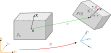
\includegraphics[width=0.8\textwidth]{figs_part2/sec3.1_introduction/rigid_body_kinematics.pdf}
        \caption{Illustration of the mapping from the reference configuration $\mathcal{F}_0$ to the current configuration $\mathcal{F}(t)$ of a rigid body. The configuration of the rigid body is specified via a translation of the center-of-mass $\mathbf{r}$ (green), and rotation $R$ (red), relative to a reference configuration with a center-of-mass located at $\mathbf{0}$. Material points $\mathbf{X}$ in the reference configuration are thus mapped to $\mathbf{x}(\mathbf{X}) = \mathbf{r} + R \mathbf{X}$. An observer that sits on the rigid body and moves with it will have a frame $E = (\mathbf{e}_1\ \mathbf{e}_2\ \mathbf{e}_3)$ (blue), which rotates relative to the fixed frame of a still observer $B = (\mathbf{b}_1\ \mathbf{b}_2\ \mathbf{b}_3)$ (orange) as $E = RB$.}
        \label{fig:rigid body kinematics}
\end{figure}

At time $t$ the location of the material point at $\mathbf{X}$ is given by $\mathbf{x}(\mathbf{X}, t)$. The latter can be related to the former as
\begin{equation} \label{eq:rigid body movement}
\mathbf{x}(\mathbf{X}, t) = \mathbf{r}(t) + R(t) \mathbf{X}, \quad  \mathbf{X} \in \mathscr{M}
\end{equation}
where $\mathbf{r}(t)$ is the location of the centre-of-mass and $R(t)$ is the rotation of the rigid body relative to its reference configuration. Now consider the second term in Eq. \ref{eq:rigid body movement},
\begin{equation}
R \mathbf{X} = \tilde{X}_i \mathbf{e}_i
\end{equation}
where $\mathbf{e}_i = R \mathbf{b}_i$ is the \textit{moving} or \textit{body} frame, which we write as $E = (\mathbf{e}_1\ \mathbf{e}_2\ \mathbf{e}_3) \in \mathbb{R}^{3 \times 3}$ and satisfies $E = RB$, and is illustrated in Fig.~\ref{fig:rigid body kinematics}. The configuration of the rigid body can thus be written as a matrix
\begin{equation}
\mathcal{F}(t) = \begin{pmatrix}
1 & \mathbf{0}^T \\
\mathbf{r}(t) & E(t)
\end{pmatrix}
\end{equation}
and we can relate it to the reference configuration as
\begin{equation}
\mathcal{F}(t) = \mathcal{F}_0  \Phi(t)
\end{equation}
where
\begin{equation}
\mathcal{F}_0 = \begin{pmatrix}
1 & \mathbf{0}^T \\
\mathbf{0} & B
\end{pmatrix}
\end{equation}
is the reference configuration and
\begin{equation} \label{eq:rigid body SE(3) state}
\Phi(t) = \begin{pmatrix}
1 & \mathbf{0}^T \\
B^T \mathbf{r} & B^T R(t) B
\end{pmatrix}
\end{equation}
is for each $t \in [0, T]$ an element of the special Euclidean group $SE(3)$ of translations and rotations. We will thus henceforth identify the configuration of the rigid body with $\Phi$, up to a global rotation of $\mathcal{F}_0$. 

The form of Eq.~\ref{eq:rigid body SE(3) state} merits some explanation. $B^T \mathbf{r}$ can be seen as the component of coefficients of $\mathbf{r}$ expressed in the fixed frame $B$, and $B^T R B$ is then the rotation $R$ in that same basis. We therefore introduce the notation $\tilde{v} = B^T \mathbf{v}$ for vectors $\mathbf{v} \in \mathbb{R}^3$. Similarly we write
\begin{equation}
\vec{v} = E^T \mathbf{v}
\end{equation}
where $\vec{v}$ is a vector $\mathbf{v} \in \mathbb{R}^3$ expressed in the moving frame $E$, with components $v_i = \mathbf{e}_i \cdot \mathbf{v}$. We thus have that $\mathbf{v} = v_i \mathbf{e}_i = \tilde{v}_i \mathbf{d}_i$.

We now derive the kinematic equations of motion of the rigid body, parametrised as a point $\Phi(t)$ in the Lie group $SE(3)$. The `velocity' of the rigid body is $\dot{\Phi}(t) \in T_{\Phi(t)} SE(3)$, a vector in the tangent space at $\Phi(t)$, which incorporates both the translation of the centre-of-mass and the rotation of the frame. As $SE(3)$ is a Lie group, there is a natural map from $T_{\Phi(t)} SE(3)$ to its Lie algebra $\mathfrak{se}(3) \cong T_{e} SE(3)$ by left (or right)-translation
\begin{equation} \label{eq:kinematics of rigid body}
\Phi^{-1} \dot{\Phi} = N \in \mathfrak{se}(3)
\end{equation}
which allows us to express the kinematics of the rigid body in terms of generalised velocities all taking values in the same Lie algebra. Equation \ref{eq:kinematics of rigid body} is an ordinary matrix differential equation and can be solved to find $\Phi(t)$ given a velocity $Y(t)$. 

We now derive the kinematic equations of motion of the rigid body in terms of more familiar quantities. Let $\vec{V}$ be the translational velocity of the center-of-mass, and $\vec{\Omega}$ the angular velocity of the rigid body, expressed in the moving frame basis. We write $N$ as
\begin{equation} \label{eq:rigid body Y}
N = \begin{pmatrix}
0 & \vec{0}^T \\
\vec{V} & \hat{\Omega}
\end{pmatrix}
\end{equation}
where $\hat{\Omega} \in \mathbb{R}^{3 \times 3}$ is the angular velocity under the hat-map. We can see $N$ as a generalised velocity, defined on the Lie algebra. The inverse of Eq.~\ref{eq:rigid body SE(3) state} is given by
\begin{equation}
\Phi^{-1} = \begin{pmatrix}
1 & \mathbf{0}^T \\
-B^T R^T \mathbf{r} & B^T R^T B
\end{pmatrix}.
\end{equation}
We now evaluate the left-hand side of Eq.~\ref{eq:kinematics of rigid body} to get
\begin{equation} \label{eq:ginv g}
\begin{aligned}
\Phi^{-1} \dot{\Phi} = \mathcal{F}^{-1} \dot{\mathcal{F}} & = \begin{pmatrix}
  0 & \vec{0}^T \\
  B^T R^T \dot{\mathbf{r}} & B^T R^T \dot{R} B
\end{pmatrix} \\
& = \begin{pmatrix}
  0 & \vec{0}^T \\
  E^T \dot{\mathbf{r}} &  E^T \dot{E} 
\end{pmatrix}
\end{aligned}
\end{equation}
Equating Eq.~\ref{eq:rigid body Y} and Eq.~\ref{eq:ginv g}, we get the kinematic equations of motion
\begin{subequations}
\begin{align}
\dot{\mathbf{r}} & = \mathbf{V} \\
\dot{E} & = E \hat{\Omega}. \label{eq:frame eom}
\end{align}
\end{subequations}
which describes the translational motion of the centre-of-mass and the rotation of the frame $E$, respectively. Equation \ref{eq:frame eom} can also be written as
\begin{equation} \label{eq:e eom rigid body}
\begin{aligned}
\dot{\mathbf{e}}_j & = \mathbf{e}_i \hat{\Omega}_{ij} \\
& = \boldsymbol{\Omega} \times \mathbf{e}_i.
\end{aligned} 
\end{equation}
where $\boldsymbol{\Omega} = \Omega_i \mathbf{e}_i$. Eq.~\ref{eq:e eom rigid body} provides a clear interpretation of the angular velocity. At time $t$ the $i$th component of the angular velocity  in the moving frame $\Omega_i(t)$ gives the rate at which the rigid body rotates around the axis $\mathbf{e}_i$.

We note that the derivations above would simplify to some extent if we let the fixed frame equal the identity matrix $B=\mathbbm{1}$, in which case $E = R$. In this section we will keep the distinction so as to make the distinction clear between the moving frame $E$ and the fixed frame $B$. It is clear that $\mathcal{F}$ (and $\mathcal{F}_0$) could also be considered Lie group-valued, and indeed $\Phi^{-1} \dot{\Phi} = \mathcal{F}^{-1} \dot{\mathcal{F}}$. In the subsequent section we will make this identification.

Now we will consider the dynamics of the rigid body. We will start with the Euler-Lagrange equations defined on the Lie group, and then show the corresponding action principle defined on the Lie algebra. The kinetic energy of the rigid body is given by
\begin{equation}  \label{eq:rigid body kinetic energy}
\begin{aligned}
\mathcal{K}(\dot{\Phi}) & = \frac{1}{2} \int_\mathscr{M} \rho^V_0(\mathbf{X}) |\dot{\mathbf{x}}(\mathbf{X})|^2  d^3 X
\end{aligned}
\end{equation}
which is here written explicitly as a function of $\dot{\Phi}$. To see this note that
\begin{equation}
\begin{pmatrix} 1 \\ \mathbf{x} \end{pmatrix} = \mathcal{F}_0 \Phi \mathcal{F}_0^{-1} \begin{pmatrix} 1 \\ \mathbf{X} \end{pmatrix}
\end{equation}
and so $\mathbf{x}$ can be seen as a function of $\Phi$. The dynamical equations of motions of a free rigid body with Lagrangian density $L : SE(3) \times TSE(3) \to \mathbb{R}$
\begin{equation}
\mathcal{L}(\Phi, \dot{\Phi}) = \mathcal{K}(\dot{\Phi})
\end{equation}
are found by invoking \textit{Hamilton's principle}
\begin{equation} \label{eq:rigid body hamiltons principle}
\delta \int_0^{T} \mathcal{L}(\Phi(t), \dot{\Phi}(t)) dt = 0
\end{equation}
under variations $\Phi(t) \to \Phi(t) + \delta \Phi (t)$, where $\delta \Phi (t)$ is a variational test function which must vanish at the temporal boundaries, and where $T$ is the upper-bound of the time-domain considered. The resulting equations of motion will be second-order equations for $\Phi$ in time. This formulation is often undesirable, as in numerical simulations errors accrue such as to push $\Phi$ out of the sub-manifold $SE(3) \subset \mathbb{R}^{4 \times 4}$. We will next formulate the corresponding equations of motion on the Lie algebra instead.

%under variations $\Phi(t) \to \Phi(t) + \delta \Phi (t)$, where $\delta \Phi (t)$ is a variational test function which must vanish at the temporal boundaries, and where $T$ is the upper-bound of the time-domain considered. The resulting equations of motion are the \textit{Euler-Lagrange} equations
%\begin{equation} \label{eq:EL equations for g}
%\frac{\partial L}{\partial \Phi_{ij}} - \frac{d}{dt} \frac{\partial L}{\partial %\dot{\Phi}_{ij}} = 0, \quad i,j=1,\dots,4.
%\end{equation}
%As a consequence of the fact that Eq.~\ref{eq:EL equations for g} is formulated directly on the Lie group, the equation is explicitly $16$-dimensional, despite the fact that $\Phi(t) \in SE(3)$ and $\text{dim}(SE(3)) = 6$. This formulation is often undesirable, as in numerical simulations this leads to errors accruing such as to push $\Phi$ out of the sub-manifold $SE(3) \subset \mathbb{R}^{4 \times 4}$. We will next formulate the corresponding equations of motion on the Lie algebra.

We have that
\begin{equation} \label{eq:rigid body kinetic energy 2}
\begin{aligned}
\mathcal{K}(\dot{\Phi}) & = \frac{1}{2} m |\dot{\mathbf{r}}|^2 + \frac{1}{2} \int_\mathscr{M} \rho^V_0(\mathbf{X}) | \dot{R} \mathbf{X}|^2 d^3 X
\end{aligned}
\end{equation}
where we have used that $\int_M \rho^V_0(\mathbf{X}) \mathbf{X} d^3 X = 0$. Now, since
\begin{equation}
\begin{aligned}
|\dot{R} \mathbf{X}| & = |\dot{E} B^T X| = |\dot{E} \tilde{X}| = |E^T \dot{E} \tilde{X}|
= |\hat{\Omega} \tilde{X}| = |\vec{\Omega} \times \tilde{X}|
\end{aligned}
\end{equation}
we see that the rotational kinetic energy is a quadratic form in terms of the angular velocity $\vec{\Omega}$. Furthermore, as $|\dot{\mathbf{r}}| = |\vec{V}|$ we can write
\begin{equation} \label{eq:K lie algebra}
\begin{aligned}
\mathcal{K}(N) & = \frac{1}{2} m |\vec{V}|^2 + \frac{1}{2} \vec{\Omega}^T \mathbb{I} \vec{\Omega}
\end{aligned}
\end{equation}
where $\mathbb{I} \in \mathbb{R}^{3 \times 3}$ is the \textit{moment of inertia} tensor, which is, unless the body is incidental to a line, positive-definite. Eq.~\ref{eq:K lie algebra} is now a function of the Lie algebra-valued $N \in \mathfrak{se}(3)$. We define the \textit{reduced Lagrangian density} $\ell : \mathfrak{se}(3) \to \mathbb{R}$
\begin{equation}
\ell(N) = \mathcal{K}(N)
\end{equation}
which coincides with the regular Lagrangian density $\mathcal{L}(\Phi, \dot{\Phi}) = \ell(N)$ when $\Phi^{-1} \dot{\Phi} = N$. To find the corresponding Hamilton's principle
\begin{equation} \label{eq:lie algebra Hamiltons principle}
\delta \int_0^T \ell(N) dt = 0
\end{equation}
defined on the Lie algebra, we identify the space of admissible variations $\delta N$ in terms of the variations on the Lie group-level $\delta \Phi$. We vary Eq.~\ref{eq:kinematics of rigid body} to find
\begin{equation}
\begin{aligned}
\delta N = - \Phi^{-1} \delta \Phi \Phi^{-1} \dot{\Phi} + \Phi^{-1} \delta \dot{\Phi}.
\end{aligned}
\end{equation}
where we used $\delta (\Phi \Phi^{-1}) = 0$ to find $\delta \Phi^{-1}$. We define the variational test function $\eta = \Phi^{-1} \delta \Phi$, which satisfies $\dot{\eta} = - N \eta + \Phi^{-1} \delta \dot{\Phi}$. We get
\begin{equation} \label{eq:lie algebra variation}
\begin{aligned}
\delta N & = \dot{\eta} + [N, \eta] \\
& = \dot{\eta} + \text{ad}_N \eta.
\end{aligned}
\end{equation}
As we will compute the corresponding variational principle for the Cosserat rod in the subsequent section, we will not go through the detailed derivation here. If the variation Eq.~\ref{eq:lie algebra Hamiltons principle} is computed using Eq.~\ref{eq:lie algebra variation}, the resulting equations of motion are
\begin{equation} \label{eq:euler poincare equation for rigid body}
\frac{d}{dt} \frac{\partial \ell}{\partial N} = \text{ad}_N^* \frac{\partial \ell}{\partial N}
\end{equation}
where $\text{ad}^*_N : \mathfrak{se}(3)^* \to \mathfrak{se}(3)^*$ is the dual of the adjoint action, defined on the dual $\mathfrak{se}(3)^*$ to the Lie algebra, and $\frac{\partial \ell}{\partial N}$ is the matrix partial derivative. Equation \ref{eq:euler poincare equation for rigid body} is the result of the \textit{Euler-Poincaré theorem} \citep{marleHenriPoincareNote2013a, marsdenIntroductionMechanicsSymmetry2013, marleHenriPoincareNote2013a, poincareFormeNouvelleEquations1901}, and is also thus referred to as the \textit{Euler-Poincaré equation}. Further details, and its derivation in the continuum case, will follow in the subsequent sections. Evaluating Eq.~\ref{eq:euler poincare equation for rigid body} leads to
\begin{subequations} \label{eq:dynamic eoms for rigid body}
\begin{align} 
\dot{\vec{V}} & = \vec{V} \times \vec{\Omega} \label{eq:V rigid body equation} \\
\mathbb{I} \dot{\vec{\Omega}} & = \mathbb{I} \vec{\Omega} \times \vec{\Omega}.
\end{align}
\end{subequations}
Eq.~\ref{eq:kinematics of rigid body} and Eq.~\ref{eq:dynamic eoms for rigid body} together fully specify the kinematics and dynamics of the free rigid body respectively. Note that Eq.~\ref{eq:dynamic eoms for rigid body} is expressed in the moving frame, and reduces to $\dot{\mathbf{V}} = 0$ and $\dot{\boldsymbol{\Omega}} = 0$ in a non-moving frame.


%We note that Eq.~\ref{eq:rigid body kinetic energy 2} is invariant under left-translation by a rigid body transformation $\Psi = (\mathbf{t} ; \tilde{R} ) \in SE(3)$. Explicitly, we have
%\begin{equation}
%\begin{aligned}
%\mathcal{K}(\Psi \dot{\Phi}) & = \frac{1}{2} m | \tilde{R} \mathbf{r} + \mathbf{t} )|^2 + \frac{1}{2} \int_\mathscr{M} \rho^V_0(\mathbf{X}) | \tilde{R} \dot{R} \mathbf{X}|^2 d^3 X \\
%& = \frac{1}{2} m | \dot{\mathbf{r}} |^2 + \frac{1}{2} \int_\mathscr{M} \rho^V_0(\mathbf{X}) | \dot{R} \mathbf{X}|^2 d^3 X = \mathcal{K}(\dot{\Phi}).
%\end{aligned}
%\end{equation}
%The left-invariance of the kinetic energy entails that we can express it in terms of Lie algebraic quantities by setting $\Psi = \Phi^{-1}$.

We will now briefly consider the case of a rigid body under the influence of an external force. As the more general case of a continuum of rigid bodies will be treated in the following section, we will leave out many mathematical details, and only state some results here to preface the results that will follow.

External forcing of the rigid body can be included by considering the more general \textit{Lagrange-D'Alembert principle} \citep{marsdenIntroductionMechanicsSymmetry2013}, which is, in integral form
\begin{equation} \label{eq:integral lagrange-dalembert for rigid bodies}
\delta \int_0^T \mathcal{L}(\Phi, \dot{\Phi})\ dt + \int_0^T (\mathbf{T}(\Phi, \dot{\Phi}))( \delta \Phi ) dt = 0
\end{equation}
where $\mathcal{L}(\Phi, \dot{\Phi})$ is the Lagrangian density of the free rigid body, and $\mathbf{T} \in T^*SE(3)$ is a covector, where its argument is the variational test function $\delta \Phi$. $\mathbf{T}$ is here a generalised external force on the rigid body, containing both the force and the moment applied on the rigid body. As shown in \cite{wisniewskiEulerPoincarReductionExternally}, Eq.~\ref{eq:integral lagrange-dalembert for rigid bodies} in reduced form leads to
\begin{equation} \label{eq:reduced integral lagrange-dalembert for rigid bodies}
\delta \int_0^T \ell (N)\ dt + \int_0^T \langle T, \eta \rangle dt = 0
\end{equation}
where $T$ is the generalised external force pulled-back onto the dual Lie algebra $\mathfrak{se}(3)^*$, $\eta$ the variational test function defined on the Lie algebra, and $\langle \cdot , \cdot \rangle : \mathfrak{se}(3)^* \times \mathfrak{se}(3) \to \mathbb{R}$ is an inner product. If we let the $\vec{f}$ and $\vec{m}$ be the external force and moment respectively, the resulting equations of motion are
\begin{subequations} 
\begin{align} 
\dot{\vec{V}} & = \vec{V} \times \vec{\Omega} + \vec{f}  \\
\mathbb{I} \dot{\vec{\Omega}} & = \mathbb{I} \vec{\Omega} \times \vec{\Omega} + \vec{m}.
\end{align}
\end{subequations}
In the following section we will generalise these equations of motion for the Cosserat rod.

\section{Geometric Cosserat rod mechanics} \label{sec:Geometric Cosserat rod mechanics}

\subsection{Cosserat rod kinematics}

\begin{figure}[t]
\centering
        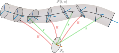
\includegraphics[width=0.8\textwidth]{figs_part2/sec7.2.1_cosserat_rod_kinematics/cosserat_F0_to_F.pdf}
        \caption{Illustration of the mapping from the reference configuration $\mathcal{F}_0$ to the current configuration $\mathcal{F}(u)$ of a Cosserat rod. The configuration of a Cosserat rod is specified by the center-line $\mathbf{r}(u),\ u \in [0, L_0]$ and a rigid body cross section attached at each $u$, related to a reference configuration $\mathcal{F}_0$, via translation (red) and rotation (red) respectively.}
        \label{fig:cosserat F0 to F}
\end{figure}

General Cosserat media can be described as a micros-tructured sub-manifold of Euclidean space. At each point-continua on the sub-manifold $n$ directors are attached, where each director can in general vary in both magnitude and direction independently. The \textit{special Cosserat rod} is an example of a Cosserat system where the one-dimensional continuum body is called the \textit{center-line} $\mathbf{r}(u)$, with two orthogonal directors at each material point $u \in [0, L_0]$, where $L_0$ is the rest length of the rod, that are constrained to be \textit{inextensible} (constant magnitude) and orthogonal. Equivalently, we can thus see the special Cosserat rod as a connected string of rigid body cross-sections. These cross-sections are represented as orthonormal frames we call the \textit{material frames} $E(u) = (\mathbf{e}_1(u)\ \mathbf{e}_2(u)\ \mathbf{e}_3(u))$, which rotate relative to each other along the material coordinate $u$. A pair $\mathbf{r}(u), E(u))$ is known as a \textit{trihedron}. See Fig.~\ref{fig:Cosserat kinematic degrees of freedom} for an illustration.

We will show that the kinematic configuration space of the Cosserat rod is the Lie group of special Euclidean transformations $SE(3)$, and then proceed to formulate its kinematic equations of motion on the corresponding Lie algebra $\mathfrak{se}(3)$.

\subsubsection*{Lie group–Lie algebra correspondence} \label{sec:Lie group–Lie algebra correspondence}

The center-of-mass of the cross-section at $u$ is given by $\mathbf{r}(u)$, and its orientation is specified by the material frame $E(u) = (\mathbf{e}_1(u)\ \mathbf{e}_2(u)\ \mathbf{e}_3(u))$, which is an orthonormal triad. As $E$ is a basis for $\mathbb{E}^3$, the vector of components in the material frame basis $\vec{v} = E^T \mathbf{v}$ will be said to be expressed in the \textit{moving frame}. The configuration of the Cosserat rod is thus specified by the center-line and material frame, which we write as
\begin{equation}
\mathcal{F}(t, u) = \begin{pmatrix}
1 & \mathbf{0}^T \\
\mathbf{r}(t, u) & E(t, u).
\end{pmatrix}
\end{equation}
We can relate rod configurations to a reference coordinate system as
\begin{equation} \label{eq:Cosserat rod from phi}
\mathcal{F}(t, u) = \mathcal{F}_0  \Phi(t, u)
\end{equation}
where
\begin{equation}
\mathcal{F}_0 = \begin{pmatrix}
1 & \mathbf{0}^T \\
\mathbf{0} & B
\end{pmatrix}
\end{equation}
is the reference coordinate system, and $\Phi(t,u) \in SE(3)$ is the transformation between the two. See Fig.~\ref{fig:cosserat F0 to F} for an illustration. In contrast the previous section, here we set the fixed frame to $B = \mathbbm{1}_{3 \times 3}$, to simplify the notation. Such that $\mathcal{F}_0 = \mathbbm{1}_{4 \times 4}$ and
\begin{equation} \label{eq:cosserat rod SE(3) state}
\Phi(t, u) = (\mathbf{r} ; E) = \begin{pmatrix}
1 & \mathbf{0}^T \\
\mathbf{r}(t,u) & E(t,u) 
\end{pmatrix} \in SE(3).
\end{equation}
where we have introduced the short-hand notation for $\Phi = (\mathbf{r} ; E)$ for $SE(3)$ elements. We thus have that $\mathcal{F}(t,u) = \Phi(t,u)$, and we will henceforth identify the Cosserat rod configuration with the group element $\Phi(t,u)$. The kinematic motion of the Cosserat rod can thus be fully specified by a space-time sheet $\Phi(t, u) \in SE(3)$ in the Lie group of special Euclidean transformations. In other words, the spatio-temporal configuration of the Cosserat rod can be described as a $2$-dimensional immersion $N \subset SE(3)$, defined by the map $\Phi : W \to SE(3)$, where we call $W = [0, T] \times [0, L_0]$ the \textit{kinematic base space}, and $N = \Phi(W)$. Therefore we call $SE(3)$ the \textit{kinematic configuration space} of the Cosserat rod, and $\Phi$ the \textit{spatio-temporal configuration} of the system. In other words, $N$ can be seen as a `sheet' in $SE(3)$, and is parametrised by the function $\Phi$. The manifolds $[0, L_0]$ and $[0, T]$ will be called the \textit{material base space} and the \textit{time domain} respectively. Furthermore, we may draw a distinction between the \textit{internal configuration space} $SO(3)$, corresponding to the material frame, and the \textit{external configuration space} $\mathbb{E}^3 \cong SE(3) / SO(3)$, corresponding to the center-line.

At a point $\Phi(t, u) \in N$, we can consider velocities in the temporal and spatial directions $\dot{\Phi}(t, u)$ and $\Phi'(t, u)$ respectively. Thus by differentiating the map $\Phi$ we get a vector field
\begin{equation}
d\Phi = \dot{\Phi} dt + \Phi' du
\end{equation}
as discussed in Sec.~\ref{sec:The Maurer-Cartan form}, where $d \Phi(t, u) \in T_{\Phi(t, u)} N$ for all $(t, u) \in W$. Here it is worth clarifying a technical point to avoid confusion. Although we say $d \Phi$ is a vector field on $N$, we have written it as a $1$-form on the kinematic base space $W$. These two notions are not contradictory. Precisely, $d\Phi$ is a \textit{$TN$-valued $1$-form on $W$}.

Via left-translation, we can relate $d \Phi$ to a $\mathfrak{se}(3)$-valued $1$-form on $W$
\begin{equation} \label{eq:xi from phi}
\xi = \Phi^{-1} d \Phi
\end{equation}
where $\xi = \Phi^* \omega$, the pull-back $\Phi^* \omega$ of the Maurer-Cartan $\omega$ form, as discussed in Sec.~\ref{sec:Sub-manifolds of homogeneous spaces}. $\xi$ contains all geometric information contained in $\Phi$, up to rigid body transformations, and as a Lie algebra-valued object $\xi$ will turn out to be easier to work with than $\Phi$ or $d \Phi$. In what follows, we will formulate the kinematics of the Cosserat rod entirely within the Lie algebra using $\xi$.

\subsubsection*{Kinematic equations of motion}

Equation \ref{eq:xi from phi} shows how to construct $\xi$ from the Lie group function $\Phi$. For our purposes it will be more relevant to go the other direction: Given a $\xi$, is there a corresponding $\Phi$? The answer can be formulated in terms of integrability. As a motivating and intuitive example from multi-variate calculus, consider a vector-valued function $\mathbf{F} : \mathbb{R}^3 \to \mathbb{R}^3$. There exists a potential $U : \mathbb{R}^3 \to \mathbb{R}$ such that $\mathbf{F} = - \nabla \cdot U$ if and only if the differential $\phi = \frac{\partial F_i}{\partial x^i} dx^i$ is \textit{exact}. In $\mathbb{R}^3$, and for Lie groups, this is equivalent to $d \phi = 0$ \footnote{This is known as the \textit{Poincaré lemma} and holds true locally for arbitrary manifolds.}. In Sec.~\ref{sec:Sub-manifolds of homogeneous spaces}, we showed that there is a $\Phi$ for which the right-hand side of Eq.~\ref{eq:xi from phi} holds true if and only if
\begin{equation} \label{eq:xi integrability condition}
d\xi + \xi \wedge \xi = 0.
\end{equation}
This is an integrability condition on $\xi$, and is a Maurer-Cartan equation on the sub-manifold $N$. As we will show, Eq.~\ref{eq:xi integrability condition} is in fact a concise expression of the kinematics of a Cosserat rod. We expand $\xi$ in terms of its temporal and spatial components
\begin{equation} \label{eq:xi = X + N}
\xi = N dt + X du
\end{equation}
where $X(t, u), N(t, u) \in \mathfrak{se}(3)$, which we write as
\begin{subequations} \label{eq:X and Y defs}
\begin{align}
X & = \{ \vec{\theta} ; \vec{\pi} \} =  \begin{pmatrix}
	0 & \vec{0}^T \\
	\vec{\theta} & \hat{\pi} 
\end{pmatrix} \label{eq:X def} \\ 
N & = \{ \vec{V} ; \vec{\Omega} \} = \begin{pmatrix}
	0 & \vec{0}^T \\
	\vec{V} & \hat{\Omega} 
\end{pmatrix}
\end{align}
\end{subequations}
where $\vec{\theta}(t,u), \vec{\pi}(t,u), \vec{V}(t,u), \vec{\Omega}(t,u) \in \mathbb{R}^3$ are vectors expressed in the material frame basis, and where we have introduced the notation $X = \{ \vec{\theta} ; \vec{\pi} \}$ as a shorthand for matrices like Eq.~\ref{eq:X def}. We will call $X$ the \textit{spatial reconstruction field} and $N$ the \textit{generalised velocity field}. Following a similar derivation as in Eq.~\ref{eq:ginv g}, we find
\begin{equation}
\Phi^{-1} d \Phi = \begin{pmatrix}
0 & \vec{0}^T \\
E^T d \mathbf{r} & E^T d E
\end{pmatrix}.
\end{equation}
\begin{figure}[t]
\centering
        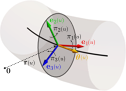
\includegraphics[width=0.65\textwidth]{figs_part2/sec7.2.1_cosserat_rod_kinematics/theta_and_pi_explanation.pdf}
        \caption{Depicts the rate-of-change along $u$ of the material frame located at $\mathbf{r}(u)$ (dashed line). The spatial derivative of the center-line (solid black line) at $u$ is $\boldsymbol{\theta}(u) = \mathbf{r}'(u)$ (yellow arrow), and $\pi_1$, $\pi_2$ and $\pi_3$ is the angular rate-of-change of the material frame around $\mathbf{e}_1$ (red), $\mathbf{e}_2$ (blue) and $\mathbf{e}_3$ (green) respectively. The analogous description holds true for $\vec{V}$ and $\vec{\Omega}$, but in time $t$ rather than material coordinate $u$.}
        \label{fig:rate-of-change of material frame}
\end{figure}
From Eq.~\ref{eq:X and Y defs} we then find that
\begin{subequations} \label{eq:dr and de}
\begin{align}
d \mathbf{r} & = \mathbf{e}_i V_i dt + \mathbf{e}_i \theta_i du \\
d \mathbf{e}_j & = \mathbf{e}_i \hat{\Omega}_{ij} dt + \mathbf{e}_i \hat{\pi}_{ij} du \label{eq:de_j}
\end{align}
\end{subequations}
which we can also write as
\begin{subequations}
\begin{align}
d \mathbf{r} & = \mathbf{V} dt + \boldsymbol{\theta} du \\
d E & = E \hat{\Omega} dt + E \hat{\pi} du. 
\end{align}
\end{subequations}
We can thus identify $\mathbf{V} = E \vec{V} = \partial_t \mathbf{r}$ as the translational velocity of the center-line, $\boldsymbol{\theta} = E \vec{\theta} = \partial_u \mathbf{r}$ as rate-of-change of the center-line along the material coordinate, and from Eq.~\ref{eq:de_j} it follows that
\begin{subequations}
\begin{align}
\dot{\mathbf{e}}_i & = \boldsymbol{\Omega} \times \mathbf{e}_i \\
\mathbf{e}_i' & = \boldsymbol{\pi} \times \mathbf{e}_i \label{eq:eom for e_i along u}
\end{align}
\end{subequations}
which show that $\boldsymbol{\Omega} = E \vec{\Omega}$ and $\boldsymbol{\pi} = E \vec{\pi}$ are the temporal and `spatial' angular velocities of the material frame respectively. The spatial part of Eq.\ref{eq:dr and de} is illustrated in Fig.~\ref{fig:rate-of-change of material frame}.  We can thus see $N$ as a generalised velocity in the Lie algebra. Equation \ref{eq:de_j} also shows how derivatives of vector functions $\mathbf{v}(t,u)$ can be expressed in terms of $\vec{v}(t,u)$ in the moving frame basis. We have
\begin{equation}
\begin{aligned}
d \mathbf{v} & = d(\mathbf{e}_i v_i) \\
& = \mathbf{e}_i (d v_i) + (d \mathbf{e}_i) v_i \\
& = E (d \vec{v}) + (E \hat{\pi} + E \hat{\Omega}) v_i \\
& = E (D_t \vec{v}\ dt + D_u \vec{v}\ du) 
\end{aligned}
\end{equation}
such that $E^T d \mathbf{v} = D_u \vec{v}\ du + D_t \vec{v}\ dt$, where
\begin{subequations} \label{eq:covariant derivatives}
\begin{align}
D_t & = \partial_t + \hat{\Omega}  \\
D_u & = \partial_u + \hat{\pi} 
\end{align}
\end{subequations}
are the spatial and temporal \textit{material derivatives} respectively. We thus have that $E^T \mathbf{v}' = D_u \vec{v}$  and $E^T \dot{\mathbf{v}} = D_t \vec{v}$.

For a given spatio-temporal velocity field $N(t,u)$, Eq.~\ref{eq:xi integrability condition} imposes a condition on the spatial reconstruction field $X(t,u)$. The resulting equations are the kinematic equations of motion. Substituting Eq.~\ref{eq:xi = X + N} into the left-hand side of Eq.~\ref{eq:xi integrability condition}
\begin{equation}
\begin{aligned}
d \xi + \xi \wedge \xi & = N' dt \wedge du + \dot{X} dt \wedge du + X N dt \wedge du  + N X dt \wedge du \\ 
& = (\dot{X} - N' + [N, X]) dt \wedge du,
\end{aligned}
\end{equation}
we get
\begin{equation} \label{eq:kinematic equations of motion in the Lie algebra}
\dot{X} = \mathcal{D}_u N.
\end{equation}
where we have defined
\begin{equation}
\mathcal{D}_u = \partial_u + \text{ad}_X.
\end{equation}
Equation \ref{eq:kinematic equations of motion in the Lie algebra} is the kinematic equation of motion for the Cosserat rod, which expresses the evolution of the spatial configuration $X$, in terms of the generalised velocity $N$. To express the kinematics in terms of the non-generalised velocities, we substitute Eq.~\ref{eq:X and Y defs} into Eq.~\ref{eq:kinematic equations of motion in the Lie algebra} to find
\begin{subequations} \label{eq:kinematic equations of motion in the moving frame}
\begin{align}
D_t \vec{\theta} & = D_u \vec{V} \\
\partial_t \vec{\pi} & = D_u \vec{\Omega}, \label{eq:pi eom}
\end{align}
\end{subequations}
which are equivalent to Eq.~\ref{eq:kinematic equations of motion in the Lie algebra} and are the kinematic equations of motion expressed in the moving frame. At the Lie group-level the corresponding equations are
\begin{subequations} \label{eq:kinematic equations of motion in the fixed frame}
\begin{align}
\dot{\mathbf{r}} & = \mathbf{V} \\
\dot{\mathbf{e}}_i & = \boldsymbol{\Omega} \times \mathbf{e}_i \label{eq:e_i eom}
\end{align}
\end{subequations} % \dot{\boldsymbol{\pi}} & = \boldsymbol{\Omega}' + \boldsymbol{\Omega} \times \boldsymbol{\pi}.
From the numerical standpoint, the benefit of Eq.~\ref{eq:pi eom} over  Eq.~\ref{eq:e_i eom} is clear. Errors in integrating the latter can in general lead to $|\mathbf{e}_i| \neq 1$ and $\mathbf{e}_i \cdot \mathbf{e}_j \neq 0$, whilst by errors in Eq.~\ref{eq:pi eom} are by construction Lie algebra-valued. In other words, errors in Eq.~\ref{eq:e_i eom} accrue in $\mathbb{R}^{3 \times 3}$, whilst errors in Eq.~\ref{eq:pi eom} accrue within the Lie group itself. Mathematically, this is due to the fact that Eq.~\ref{eq:kinematic equations of motion in the Lie algebra} is defined on the linear space $W \times \mathfrak{se}(3)$, as opposed to Eq.~\ref{eq:kinematic equations of motion in the fixed frame} which is defined on the non-linear space $G \times TG$.

\subsubsection*{Types of deformations} \label{sec:deformation types}

Fig.~\ref{fig:Examples of Cosserat deformations} shows the various types of deformations that are kinematically possible for the Cosserat rod. Here we will describe how these deformations are encoded in $\vec{\theta}$ and $\vec{\pi}$. Since $\boldsymbol{\theta} = \mathbf{r}'$ we have that if $\vec{\theta}(u) \propto (1\ 0\ 0)$ then the material frame at $u$, pointing in the direction $\mathbf{e}_1(u)$ is aligned with the center-line. We thus see that $\vec{\theta}$ measures the \textit{shear} of the rod. Note that this is because $\vec{\theta}$ is expressed in the moving frame; $\boldsymbol{\theta}$ does not contain any information about the shear.

\textit{Twist} is the rotation of the material frame around $\mathbf{e}_1$, and the rate of twist along the material coordinate is given by $\pi_1$. Similarly, the rotation of the material frame around $\mathbf{e}_2$ and $\mathbf{e}_3$ are given by $\pi_2$ and $\pi_3$ respectively, as depicted in Fig.~\ref{fig:rate-of-change of material frame}.

In a non-moving frame the \textit{bending} of the center-line is encoded in $\mathbf{r}$, likewise $\boldsymbol{\theta}$. In the moving frame it is encoded in both $\vec{\theta}$ and $\vec{\pi}$ simultaneously. For instance, is $\vec{\theta}$ is constant along $u$ and $\pi_2$ or $\pi_3$ are non-zero along $u$, then the rod is bending.

In general velocities $\vec{V}$ will cause the Cosserat to \textit{extend}. Locally, the extension is described by the scalar $h(u) =  \left| \mathbf{r}' \right| = |\vec{\theta}|$, which can be seen as the square root of the metric on the center-line induced by the Euclidean metric on $\mathbb{R}^3$. Using $h$ we can define an arc-length coordinate as
\begin{equation}
ds = h(u) du
\end{equation}
which relates the arc-length increment $ds$ to the material length increment $du$. In the arc-length parametrisation we thus have $ \left| \frac{\partial \mathbf{r}}{\partial s} \right| = 1$ for all $s \in [0, L]$ where
\begin{equation}
L[h(u)] = \int_0^{L_0} h(u) du
\end{equation}
is the total arc-length of the center-line. $h(u)$ thus measures the local extension of the rod, where $h(u) = |\vec{\theta}| = 1$ indicates that the rod is not suffering an extension at $u$.

We define a unit-vector tangent to the center-line $\mathbf{t} = \boldsymbol{\theta} / |\boldsymbol{\theta}|$. The \textit{curvature} of the center-line is then a scalar defined as
\begin{equation} \label{eq:scalar curvature}
\kappa = |\mathbf{t}'|.
\end{equation}
In the literature it is more common to define the curvature in terms of the arc-length parametrisation, which we write as $\tilde{\kappa} = |\partial_s \mathbf{t}| = |\partial_s^2 \mathbf{r}|$.

%In practice, for the aforementioned reasons on the benefits of working with Lie algebra-valued (rather than Lie group-valued) objects, we will use Eq.~\ref{eq:kinematic equations of motion in the Lie algebra} or Eq.~\ref{eq:kinematic equations of motion in the moving frame} rather than Eq.~\ref{eq:kinematic equations of motion in the fixed frame}.

%Although equivalent, it is important to note the practical and theoretical differences in integrating Eq.~\ref{eq:kinematic equations of motion in the fixed frame}, as compared to integrating Eq.~\ref{eq:kinematic equations of motion in the Lie algebra} or Eq.~\ref{eq:kinematic equations of motion in the moving frame}. In the latter, 

\subsubsection*{Reconstructing the Cosserat rod from $\xi$} \label{sec:reconstructing the cosserat rod}

Solving Eq.~\ref{eq:kinematic equations of motion in the Lie algebra}, for a given velocity $N$, yields the Lie algebra-valued $1$-form $\xi$ which contains, in infinitesimal form, information from which the Cosserat rod $\mathcal{F}$ can be reconstructed. Firstly, recall that we can reconstruct $\Phi$, the representation of the Cosserat rod as a space-time sheet in the Lie group, from $\xi$ using Eq.~\ref{eq:xi from phi}. Secondly, from Eq.~\ref{eq:Cosserat rod from phi} we note that $\Phi^{-1} d \Phi = \mathcal{F}^{-1} d \mathcal{F}$. Therefore we can reconstruct the Cosserat rod from $\xi$ by solving the equation
\begin{equation}
d \mathcal{F} = \mathcal{F} \xi.
\end{equation}
We will now put the above into a form solvable as a matrix ordinary differential equation. By expanding $\mathcal{F}^{-1} d \mathcal{F}$ into its components, and from Eq.~\ref{eq:xi = X + N} we find that
\begin{subequations} \label{eq:reconstruction of F eqs}
\begin{align}
\mathcal{F}^{-1} \mathcal{F}' & = X \label{eq:phi u matrix ode} \\
\mathcal{F}^{-1} \dot{\mathcal{F}} & = Y. \label{eq:phi t matrix ode}
\end{align}
\end{subequations}
For fixed $t = \bar{t}$ and given initial conditions Eq.~\ref{eq:phi u matrix ode} can be used to find $\mathcal{F}(u,\bar{t})$ for $u \in [0, L_0]$, and for fixed $u = \bar{u}$ and given initial conditions Eq.~\ref{eq:phi t matrix ode} can be used to find $\mathcal{F}(\bar{u}, t)$ for $t \in [0, T]$. We can therefore trace out and reconstruct $\mathcal{F}(t,u)$ by repeatedly solving Eqs.~\ref{eq:phi u matrix ode} and \ref{eq:phi t matrix ode}. Due to Eq.~\ref{eq:xi integrability condition}, which ensures that $d \mathcal{F}$ is an `exact' differential, the resulting $\mathcal{F}(t,u)$ is invariant with respect to the particular path in $(t,u)$-space taken to reconstruct it. Therefore, a suitable scheme to reconstruct $\mathcal{F}$ is to first reconstruct the Cosserat rod in time along $u=0$ by solving
\begin{equation} \label{eq:1st step reconstruction}
\bar{\mathcal{F}}(t) = \bar{\mathcal{F}}(t) \dot{\bar{\mathcal{F}}}(t),
\end{equation}
with initial condition $\bar{\mathcal{F}}(0) = \mathcal{F}^{0,0}$, where the latter corresponds to choosing values for $\mathbf{r}(0,0)$ and $E(0,0)$. Secondly, for any given time $t = \bar{t}$ we can reconstruct the Cosserat rod in space by solving
\begin{equation}
\mathcal{F}(u,\bar{t}) = \mathcal{F}(u, \bar{t}) \mathcal{F}(u, \bar{t})',
\end{equation}
with initial condition $\mathcal{F}(0, \bar{t}) = \bar{\mathcal{F}}(\bar{t})$. See App.~\ref{app:Reconstructing the Cosserat rod from xi} for a detailed description of the numerical algorithm.

\subsubsection*{Closed Cosserat rods}

Thus far we have considered $\textit{open}$ Cosserat rods, for which $\mathbf{r}(0) \neq \mathbf{r}(L_0)$ and $E(0) \neq E(L_0)$. For \textit{closed} Cosserat rods the material coordinate $u \in [0, L_0]$ is periodic in its domain, and the center-line and material frame must also be periodic and continuous in $u$. Although seemingly complicated, the following derivations fill result in showing that the case of a closed Cosserat can be in practice treated equivalently to an open Cosserat rod.

A closed rod implies that
\begin{equation} \label{eq:periodic X}
X(0) = X(L_0).
\end{equation}
However, Eq.~\ref{eq:periodic X} is only a necessary, but not sufficient, condition for the rod to close. The sufficient condition is for the constraint
\begin{equation}
\mathcal{F}(0, t) = \mathcal{F}(L_0, t)
\end{equation}
to hold for all $t$. This is an integral constraint on $X$, as formally we can write
\begin{equation}
\mathcal{F}(L_0, t) = \mathcal{F}(0, t) \mathscr{U} \exp \left\{ \int_0^{L_0} X du  \right\}
\end{equation}
where $\mathscr{U}$ denotes a $u$-ordered integral. The integral constrain on $X$ is therefore
\begin{equation} \label{eq:closed rod integral constraint}
\mathscr{U} \exp \left\{ \int_0^{L_0} X du  \right\} = \mathbbm{1}.
\end{equation}
However, if $N$ is a smooth function of $u$, the kinematic equations of motion will preserve Eq.~\ref{eq:closed rod integral constraint}. This means that if the rod is initialised to obey Eq.~\ref{eq:closed rod integral constraint} at $t=0$, it will continue to do so for all $t$.

In practice, in order to simulate a closed filament we must thus first construct on the Lie group-level a periodic $\mathcal{F}(u, 0)$, and then use Eq.~\ref{eq:phi u matrix ode} to find $X(u, 0)$ that obeys Eq.~\ref{eq:closed rod integral constraint}.

\subsection{Cosserat rod dynamics} \label{sec:Cosserat rod dynamics}

\subsubsection*{Constitutive dynamics} \label{sec:Cosserat rod constitutive dynamics}

Thus far we have considered the Cosserat rod abstractly as a sub-manifold of $SE(3)$. Physically, the Cosserat rod is a kinematic approximation of a deformable and slender tube. Let $\mathscr{M} = D \times [0, L_0] \subset \mathbb{R}^3$ be the reference configuration of such a tube, where $D \subset \mathbb{R}^2$ is the cross-section of the tube and is of arbitrary shape. Let $\mathbf{X} \in \mathscr{M}$ denote the material coordinates of $\mathscr{M}$, such that $X_1 \in [0, L_0]$ and $(X_2, X_3) \in \mathscr{D}$ and for simplicity let $\rho^V_0$ be a constant mass density per unit material volume at each $\mathbf{X}$. At time $t$ the location of the material point at $\mathbf{X}$ is given by $\mathbf{x}(\mathbf{X}, t)$, which are the deformed coordinates. We define $(X_2, X_3)$ to be in the centre-of-mass of the cross-section, such that $\int_{\mathscr{D}} X_\gamma d X_2 d X_3 = 0,\ \gamma = 2,3$.

The Cosserat rod models the slender deformable tube under the kinematic assumption that the material fibres that run radially from the center of $\mathcal{D}$ to its edge are fixed. In other words we impose that
\begin{equation} \label{eq:cosserat rod kinematic assumption}
\mathbf{x}(\mathbf{X}, t) = \mathbf{r}(t, u) + X_\gamma \mathbf{e}_\gamma(t, u), \quad \gamma = 2,3
\end{equation}
where $\mathbf{r}(t, u)$ is the center-line of the rod and where $u = X_1$ is the material coordinate along the center-line. The three-dimensional tube has thus been replaced with the Cosserat rod, which only has one spatial dimension. In this coarse-graining, the two missing spatial dimensions have been replaced by rigid body cross-sections attached at each $u \in [0, L_0]$, with orientation specified by the two directors $\mathbf{e}_2$ and $\mathbf{e}_3$.

As in Sec.~\ref{sec:Introduction - rigid body} we formulate the dynamics of the Cosserat rod via a Lagrangian formulation. We will again be using a reduction of the Lagrangian to construct dynamics defined on the Lie algebra. We derive the constitutive dynamics by first computing the kinetic energy of the rod in terms of its generalised velocity $N = \{ \vec{V} ; \vec{\Omega} \}$.

We assume that the dynamics is defined by a Lagrangian density of the form $\mathcal{L}(\Phi, d \Phi)$, and that its kinetic energy term is given by
\begin{equation} \label{eq:lagrangian of tube}
\int_0^{L_0} \mathcal{K}(\dot{\Phi})\ du = \frac{1}{2} \int_\mathscr{M} \rho^{V}_0 | \dot{\mathbf{x}} |^2\ d^3 X
\end{equation} 
where $\mathcal{K}$ is the kinetic energy density along the material coordinate $u$. Substituting in Eq.~\ref{eq:cosserat rod kinematic assumption} we get
\begin{equation} \label{eq:K intermediate result 1}
\int_0^{L_0} \mathcal{K}(\dot{\Phi})\ du = \frac{1}{2} \int_0^{L_0} \rho_0 |\mathbf{V}|^2 du + \frac{1}{2} \rho_0^V \int_\mathscr{M} \mathbf{V} \cdot \dot{\mathbf{e}}_\gamma X_\gamma d^3 X  + \frac{1}{2} \rho_0^V \int_\mathscr{M} |X_\gamma \dot{\mathbf{e}}_\gamma|^2 d^3 X
\end{equation} 
where $\rho_0 = A \rho^{V}_0$ is the mass density per unit material length, and $A = \int_D d X_2 dX_3$ is the area of the cross-section, and we have used $\dot{\mathbf{r}} = \mathbf{V}$. The second term in Eq.~\ref{eq:K intermediate result 1} vanishes when the integral over $D$ is evaluated. To evaluate the third term, let $\bar{\mathbf{X}} = X_\gamma \mathbf{e}_\gamma$, and note that $\mathbf{e}_i = \boldsymbol{\Omega} \times \mathbf{e}_i$, and so
\begin{equation}
|X_\gamma \dot{\mathbf{e}}_\gamma|^2 = |X_\gamma \boldsymbol{\Omega} \times \mathbf{e}_\gamma|^2 = |\boldsymbol{\Omega} \times \bar{\mathbf{X}}|^2 = |E (\vec{\Omega} \times \bar{\vec{X}})|^2 = |\vec{\Omega} \times \vec{\bar{X}}|^2
\end{equation}
where we used $(E\vec{\Omega}) \times (E\vec{\bar{X}}) = E (\vec{\Omega} \times \vec{\bar{X}})$. As $|(\vec{\Omega} \times \vec{\bar{X}})|^2$ is a quadratic form in $\vec{\Omega}$, we can write
\begin{equation}
\frac{1}{2} \rho_0^V \int_\mathscr{M} |X_\gamma \dot{\mathbf{e}}_\gamma|^2 d^3 X = \frac{1}{2} \int_0^{L_0} \vec{\Omega}^T \mathbb{I} \vec{\Omega} du
\end{equation}
where $\mathbb{I}$ is the cross-sectional moment-of-inertia per unit material length. We can thus write the kinetic energy of the Cosserat rod as $K(N) = \int_0^{L_0} \mathcal{K}(N) du$ where 
\begin{equation} \label{eq:reduced kinetic energy}
\mathcal{K}(N)  = \frac{1}{2} \rho_0 |\vec{V}|^2 +  \frac{1}{2} \vec{\Omega}^T \mathbb{I} \vec{\Omega}
\end{equation}
is the kinetic energy per material unit length, which is now explicitly a function of the generalised velocity $N$.

Having established that the kinetic energy of the Cosserat rod has a reduced form, we now assume that we have a reduced Lagrangian density of the form
\begin{equation} \label{eq:cosserat reduced lagrangian}
\ell(\xi) = \mathcal{K}(N) - \mathcal{U}(X)
\end{equation}
where $\mathcal{U}(X)$ is the potential energy per material unit length of a given spatial configuration $X = \{ \vec{\theta} ; \vec{\pi} \}$, and $\ell(\xi)$ is here a Lagrangian density defined on the Lie algebra. The reduced Lagrangian density satisfies $\ell(\xi) = \mathcal{L}(\Phi, d\Phi)$ when $\xi = \Phi^{-1} d \Phi$. 

The reduced Lagrangian density Eq.~\ref{eq:cosserat reduced lagrangian} is explicitly invariant under Galilean transformations, as it is written in terms of the invariant quantities $X$ and $N$. Physically, the fact that a Lagrangian $\mathcal{L}(\Phi, d\Phi)$ admits a reduction $\ell(\xi)$ entails that only differential deformations couple to the dynamics. In other words the Lagrangian is really only a function of the tangent space $\mathcal{L}(d \Phi)$. We will henceforth omit the argument in $\Phi$ when the Lagrangian density admits a reduced form.

%The Lagrangian formalism motivates the definition of a momentum, conjugate to the generalised velocity $Y$, which take values in the dual $\mathfrak{se}(3)^*$ to the Lie algebra $\mathfrak{so}(3)$. $\mathfrak{se}(3)^*$ is the space of linear operators on $\mathfrak{se}(3)$, and in matrix form can be written as \citep{fultonRepresentationTheoryFirst2013}
%\begin{equation}
%\mathfrak{se}(3)^* = \{ -A^T\ |\ A \in \mathfrak{se}(3) \}
%\end{equation}


The \textit{generalised conjugate momentum} of the Cosserat rod is
\begin{equation}
S := \frac{\partial \ell}{\partial N}  = \frac{\partial \mathcal{K}}{\partial N} = \begin{pmatrix}
0 & \vec{P}^T \\ 
\vec{0} & \vec{L}^T
\end{pmatrix}  \in \mathfrak{se}(3)^*
\end{equation}
where $\vec{P} = \rho_0 \vec{V}$ and $\vec{L} = \mathbb{I} \vec{\Omega}$. It will become clear that $\vec{P}$ is the linear momentum of the center-line per unit material length, and $\vec{L}$ is the angular momentum per unit material length of the material frame. We use the short-hand $S = \{ \vec{P} ; \vec{L} \}$ as for Lie algebra elements. The matrix derivative $\frac{\partial \ell}{\partial N}$ is evaluated only with respect to the non-zero components of $N$, for which we have $S_{ji} = \frac{\partial \ell}{\partial N_{ij}}$, and $S_{ji} = 0$ otherwise. $S$ can be seen to take values in the dual Lie algebra $\mathfrak{se}(3)^*$, which is the space of linear operators $\mathfrak{se}(3) \to \mathbb{R}$ on the Lie algebra. To see this, note that $\mathcal{K}(N)$ can be written as
\begin{equation}
\mathcal{K}(N) = \frac{1}{2} \langle N, P \rangle
\end{equation}
where $\langle \cdot , \cdot \rangle : \mathfrak{se}(3) \times \mathfrak{se}(3)^* \to \mathbb{R}$ is an inner product defined as
\begin{equation}
\langle A , B \rangle =  \vec{a} \cdot \vec{b} + \vec{m} \cdot \vec{n}
\end{equation}
where $A = \{\vec{a}; \vec{m}\} \in \mathfrak{se}(3)$ and $B = \{\vec{b}; \vec{n}\} \in \mathfrak{se}(3)^*$. Similarly, we can define a \textit{generalised stress}, conjugate to the spatial configuration $X$, as
\begin{equation}
Q := \frac{\partial \mathcal{U}}{\partial X}.
\end{equation}
We write its components as $Q = \{ \vec{F} ; \vec{M} \}$ where
\begin{subequations} \label{eq:F_i and M_i from U}
\begin{align}
F_i = \frac{\partial \mathcal{U}}{\partial \theta_i} \\
M_i = \frac{\partial \mathcal{U}}{\partial \pi_i} 
\end{align}
\end{subequations}
are, as will be shown, the force on the center-line and the moment on the material frame respectively.

To find dynamic equations of motion for $P$ and $Q$, we invoke Hamilton's principle that variations
\begin{equation} \label{eq:variation of ell}
\delta \int_W \ell(\xi)\ dt \wedge du
\end{equation}
must vanish, where $\ell(\xi)$ is again the reduced Lagrangian density for the system. As for the rigid body in Sec.~\ref{sec:Introduction - rigid body}, we must first derive the permissible form of the variations. We first consider the Lagrangian density $\mathcal{L} : SE(3) \times TSE(3) \to \mathbb{R}$ defined on the Lie group, which satisfies $\mathcal{L}(\Phi, d \Phi) = \ell(\xi)$ when $\Phi^{-1} d \Phi = \xi$. The Euler-Lagrange equations are found by imposing
\begin{equation} \label{eq:hamiltons principle}
\delta \int_W \mathcal{L}(\Phi, d \Phi)\ dt \wedge du = 0
\end{equation}
under variations $\Phi \to \Phi + \delta \Phi$, where $\delta \Phi(t,u) \in TSE(3)$ is a variational test function which must vanish at the temporal boundaries. We will now assume that the Lagrangian density can be written as a function $\mathcal{L} = \mathcal{L}(d \Phi)$, purely in terms of the tangent vectors $d \Phi$. Repeating similar steps as in Sec.~\ref{sec:Introduction - rigid body}, we vary $\xi = \Phi^{-1} d \Phi$ to get
\begin{equation}
\delta \xi = - \Phi^{-1} \delta \Phi \Phi^{-1} d \Phi + \Phi^{-1} \delta (d \Phi).
\end{equation}
We define the variational test function $\eta = \Phi^{-1} \delta \Phi$, which satisfies $d \eta = - N \eta + \Phi^{-1} \delta (d \Phi)$, to get
\begin{equation}
\begin{aligned}
\delta \xi & = d \eta + \text{ad}_\xi \eta \\
& = (\dot{\eta} + \text{ad}_N ) dt + (\eta' + \text{ad}_X \eta) du \\
& = \delta X du + \delta N dt
\end{aligned}
\end{equation}
We now proceed to evaluate Eq.~\ref{eq:variation of ell}. We first note that since
\begin{equation}
\begin{aligned}
\delta \ell & = \frac{\partial \ell}{\partial X_{ij}} \delta X_{ij} + \frac{\partial \ell}{\partial N_{ij}} \delta N_{ij} \\ 
& = \langle S, \delta N \rangle  - \langle Q, \delta X \rangle,
\end{aligned} 
\end{equation}
we have
\begin{equation} \label{eq:variation of ell derivation}
\begin{aligned}
& \delta \int_W \ell(\xi)\ dt \wedge du  = \int_W \left\{ \langle  \delta N,  S \rangle  - \langle \delta X, Q \rangle  \right\} dt \wedge du  \\
& \quad = \int_W \left\{   \langle \dot{\eta} + \text{ad}_N \eta, S \rangle  - \langle  \eta' + \text{ad}_X \eta, Q \rangle  \right\}  dt \wedge du \\
& \quad = \int_W \left\{ \left\langle \eta, \left( - \frac{\partial}{\partial t} - \text{ad}_N^* \right) S \right\rangle  - \left\langle  \eta, \left( - \frac{\partial}{\partial u} - \text{ad}_X^* \right) Q \right\rangle  \right\}  dt \wedge du \\
& \quad \ + \int_0^{L_0} \left[ \langle \eta, S \rangle \right]_0^T du - \int_0^T \left[ \langle \eta, Q \rangle \right]_0^{L_0} dt \\
& \quad = 0
\end{aligned}
\end{equation}
where we used integration-by-parts and where $\text{ad}_A^* : \mathfrak{se}(3)^* \to \mathfrak{se}(3)^*$ is the dual of the adjoint action, defined as $\langle \text{ad}_A^* B , C \rangle = -\langle B, \text{ad}_A C \rangle$. We impose that the variation vanishes at the temporal boundaries, to get
\begin{subequations} \label{eq:dynamics eoms}
\begin{align}
\mathcal{D}^*_t S & = \mathcal{D}^*_u Q \\
Q & = 0, \quad u = 0, L_0 \label{eq:Q boundary conditions}
\end{align}
\end{subequations}
where
\begin{subequations}
\begin{align}
\mathcal{D}^*_t & = \partial_t + \text{ad}_N^*  \\
\mathcal{D}^*_u & = \partial_u + \text{ad}_X^* 
\end{align}
\end{subequations}
which was first derived in \citep{holmMatrixGstrands2014, giusteriSimulationViscoelasticCosserat2021}, where Eq.~\ref{eq:Q boundary conditions} arises from imposing that $\int_0^T \left[ \langle Q, \eta \rangle \right]_0^{L_0} dt = 0$ for arbitrary variations $\eta$.  As $Q = Q(X)$, Eq.~\ref{eq:Q boundary conditions} is a boundary condition on $X$. Equation \ref{eq:dynamics eoms} is the local balance law of linear and angular momentum in the absence of external forces, and together with Eq.~\ref{eq:kinematic equations of motion in the Lie algebra} completely determines the constitutive kinematics and dynamics of a Cosserat rod. These equations are first-order partial differential equations in both time $t$ and space $u$. The corresponding equations of motion for a closed rod are identical, with the exception that Eq.~\ref{eq:Q boundary conditions} no longer applies.

We now evaluate Eq.~\ref{eq:dynamics eoms} in terms of the components of $S$, $Q$, $X$ and $Y$. To do this we must first compute action of the dual adjoint $\text{ad}_B^*$. As $\text{ad}_B$ is a linear operator, it can be represented in matrix form as
\begin{equation} \label{eq:SE(3) dual adjoint}
[\text{ad}_A] = \begin{pmatrix}
\hat{n} & \hat{a} \\
0_{3 \times 3} & \hat{n}
\end{pmatrix} \in \mathbb{R}^{6 \times 6}
\end{equation}
where $A = \{ \vec{a} ; \hat{n} \}$ and acts as $[\text{ad}_A] \vec{B}$, where we have represented $B = \{ \vec{b} ; \vec{m} \}$ as vectors $\vec{B} = ( {\vec{b}}^T {\vec{m}}^T )^T \in \mathbb{R}^6$. Now we have
\begin{equation}
\begin{aligned}
\langle B, \text{ad}_A C \rangle & = \vec{B}^T [\text{ad}_A] \vec{C} \\
 & = - ([\text{ad}_A^*] \vec{B} )^T \vec{C} \\
 & = - \vec{B}^T [\text{ad}_A^*]^T \vec{C}.
\end{aligned}
\end{equation}
We thus have that
\begin{equation} \label{eq:dual adjoint}
[\text{ad}_A^*] = -[\text{ad}_A]^T = \begin{pmatrix}
\hat{n} & 0_{3 \times 3} \\
 \hat{a} & \hat{n}
\end{pmatrix} \in \mathbb{R}^{6 \times 6} 
\end{equation}
where we used $\hat{a}^T = - \hat{a}$ for anti-symmetric matrices. Using Eq.~\ref{eq:dual adjoint} we get
\begin{subequations} \label{eq:dynamics in terms of V and L}
\begin{align}
 D_t \vec{P} & = D_u \vec{F} \\
D_t \vec{L} & = D_u \vec{M} + \vec{\theta} \times \vec{F}  \\
\vec{M} & = 0, \quad u = 0, L_0 \\
\vec{F} & = 0, \quad u = 0, L_0
\end{align}
\end{subequations}
where we used the definitions of $S$, $Q$, $X$ and $Y$ and the covariant derivative. In the non-moving frame the equations of motion are
\begin{subequations} \label{eq:dynamics in terms of V and L fixed frame}
\begin{align}
\dot{\mathbf{P}} & = \mathbf{F}' \label{eq:linear force balance} \\
\dot{\mathbf{L}} & = \mathbf{M}' + \mathbf{r}' \times \mathbf{F} \label{eq:moment balance fixed frame}
\end{align}
\end{subequations}
where $\mathbf{F} = \mathbf{M} = 0$ at $u = 0, L_0$, which are the classical force and moment balance equations for a Cosserat rod \citep{cosseratTheoryDeformableBodies1909, simoGeometricallyexactRodModel1991}. Here we see explicitly that $\mathbf{F}$ and $\mathbf{M}$ is a constitutive force on the center-line and a constitutive moment on the material frame respectively, with dimensions of force and moment respectively. We can also identify $\mathbf{P}$ as the linear momentum per unit material length of the center-line, and $\mathbf{L}$ as the angular momentum per unit material length of the material frame. The second term in Eq.~\ref{eq:moment balance fixed frame} is the moment exerted on the material frame by the force. Note that linear force balance Eq.~\ref{eq:linear force balance} is  the $1$-dimensional analogue of the Cauchy momentum equation Eq.~\ref{eq:Cauchy momentum equation}, where the force that arise from constitutive stresses is here $\mathbf{F}$. We thus see that the physical description of the Cosserat rod is consistent with classical continuum mechanics. For a discussion on how the dimensions of the kinematic and dynamic quantities are arrived at, as well as how to nondimensionalise the dynamics, see App.~\ref{app:Nondimensionalisation of the Cosserat rod}.

The generalised momentum can be written in a compact form as
\begin{equation} \label{eq:S = MN}
\vec{S} = \mathsf{M} \vec{N} 
\end{equation}
where
\begin{equation} \label{eq:Cosserat rod mass matrix}
\mathsf{M} = \begin{pmatrix}
\rho_0 \mathbbm{1}_{3 \times 3} & 0_{3 \times 3} \\
0_{3 \times 3} & \mathbbm{I}
\end{pmatrix}
\end{equation}
is a generalised mass matrix. Similarly, in many applications the constitutive potential energy density can be written as a quadratic form
\begin{equation} \label{eq:U quadratic form}
\mathcal{U} = \frac{1}{2} (\vec{X} - \vec{X}_0)^T \mathsf{K} (\vec{X} - \vec{X}_0)
\end{equation}
where $\mathsf{K}$ is a symmetric and positive-definite matrix, representing the elastic stiffness of the rod, and $\vec{X}_0$ is a given rest state. In which case the generalised stress can be written as
\begin{equation}
\vec{Q} = \mathsf{K} \vec{X}.
\end{equation}
Henceforth we will write write $S = \mathsf{M} N$ and $Q = \mathsf{K} X$, where the action of matrices like $\mathsf{M}$ are to be understood in the sense of Eq.~\ref{eq:S = MN}.

\subsubsection*{Body forces and non-conservative dynamics} \label{sec:Body forces and non-conservative dynamics}

\begin{comment}

The following is a generalisation of the derivations in \citep{wisniewskiEulerPoincarReductionExternally, poincareFormeNouvelleEquations1901, marleHenriPoincareNote2013} for continuum systems. 

In the preceding sections we considered a stress $Q = \frac{\partial \mathcal{U}}{\partial X}$, leading to conservative dynamics. In general, the dynamics does not have to be variational (i.e. derived from a potential $\mathcal{U}$). When this is not the case, we say that the dynamics is \textit{non-conservative}. Furthermore external or internal \textit{body} forces and moments, like gravity and friction, are absent in Eq.~\ref{eq:dynamics eoms}.

We will first treat the case of variational dynamics with body forces. We consider a general Lagrangian density $\mathcal{L}(\Phi, d \Phi)$ that cannot be written in a purely reduced form. However we can construct a partially reduced Lagrangian $\ell(\Phi, \xi)$ that satisfies $\mathcal{L}(\Phi, d \Phi) = \ell(\Phi, \xi)$ when $\xi = \Phi^{-1} d \Phi$. Following \citep{marleHenriPoincareNote2013, poincareFormeNouvelleEquations1901, wisniewskiEulerPoincarReductionExternally}, Hamilton's principle is as before
\begin{equation}
\delta \int_W \ell(\Phi, \xi)\ dt \wedge du = 0
\end{equation}
where, once the variational operator has been applied on the integrand, the variational test functions take values in the Lie group and Lie algebra for the two arguments respectively
\begin{equation} \label{eq:variation of non-reduced lagrangian}
\begin{aligned}
\int_W \left\{   \langle \delta N, S \rangle  - \langle \delta X, Q \rangle  \right\} dt \wedge du + \int_W \frac{\partial \ell}{\partial \Phi_i} \delta \Phi_i dt \wedge du
\end{aligned}
\end{equation}
where the first term comes from the reduced part of the Lagrangian, where $\Phi_i,\ i=1,\dots,\text{dim}(SE(3))$ are some given coordinates on $SE(3)$ and we sum over $i$. An example of such coordinates could be $\Phi_i = (\mathbf{b}_1 \cdot \mathbf{r}, \mathbf{b}_2 \cdot \mathbf{r}, \mathbf{b}_3 \cdot \mathbf{r}, \varphi, \theta, \psi)$, where $(\varphi, \theta, \psi)$ are the Euler angles for $SO(3)$ rotations.

We can rewrite the integrand of the second term in Eq.~\ref{eq:variation of non-reduced lagrangian} as
\begin{equation}
\mathbf{T}(\delta \Phi) = \frac{\partial \ell}{\partial \Phi_i} \delta \Phi_i.
\end{equation}
We can thus identify $\mathbf{T} \in T^* SE(3)$ is a covector field acting on the variational test function $\delta \Phi$, and we will call it the \textit{generalised body force}.

The first term of Eq.~\ref{eq:variation of non-reduced lagrangian} evaluates to Eq.~\ref{eq:variation of ell derivation} as before. To find the dynamical equations of motion we must massage the second term in Eq.~\ref{eq:variation of non-reduced lagrangian} so that the integrand is of the form $\langle \eta, \cdot \rangle$. We write
\begin{equation} \label{eq:T derivation}
\begin{aligned}
\int_W \mathbf{T}(\delta \Phi)\ dt \wedge du & = \int_W \mathbf{T}( \Phi \eta )\ dt \wedge du \\
& = \int_W \mathbf{T}( L_\Phi \eta )\ dt \wedge du \\
& = \int_W \langle \eta, T \rangle \ dt \wedge du \\
\end{aligned}
\end{equation}
where we used $\eta = \Phi^{-1} \delta \Phi$, and where $T = L^*_\Phi \mathbf{T}$ is the generalised body force mapped to the dual Lie algebra and is thus a map $T : W \to \mathfrak{se}(3)^*$, and $L^*_\Phi : T^*_\Phi SE(3) \to \mathfrak{se}(3)^*$ is a mapping from the cotangent bundle to the dual Lie algebra defined as $\mathbf{T}( L_\Phi \eta ) = \langle L^*_\Phi \mathbf{T}, \eta \rangle$.

%Explicitly, we have \citep{marleHenriPoincareNote2013, poincareFormeNouvelleEquations1901, wisniewskiEulerPoincarReductionExternally}
%\begin{equation}
%T = L_\Phi^* \mathbf{T} = \mathbf{T} (\Phi^{-1})^T.
%\end{equation}

The resulting dynamical equations of motion, which now include arbitrary body forces and moments, are
\begin{subequations} \label{eq:dynamics eoms with body forces}
\begin{align}
\mathcal{D}^*_t S & = \mathcal{D}^*_u Q + T \\
Q & = 0, \quad u = 0, L_0. 
\end{align}
\end{subequations}
The analogous equation for non-continuum systems can be found Eq.~4 in \cite{marleHenriPoincareNote2013a} and Eq.~6 in \citep{wisniewskiEulerPoincarReductionExternally}. Expressed in non-Lie algebraic terms, by setting $\vec{T} = \{ \vec{f} ; \vec{m} \}$, the equations of motion in the moving frame are
\begin{subequations} \label{eq:dynamics in terms of V and L with body forces}
\begin{align}
D_t \vec{P} & = D_u \vec{F} + \vec{f} \\
D_t \vec{L} & = D_u \vec{M} + \vec{\theta} \times \vec{F} + \vec{m}
\end{align} \label{eq:dynamics in terms of V and L in moving frame with body forces}
\end{subequations}
where $\vec{f}$ and $\vec{m}$ are the body force and moment respectively, with units of force and moment per unit material length respectively, and $\vec{F} = \vec{M} = 0$ at $u \in 0, L_0$ as before. Finally, in the non-moving frame, we have
\begin{subequations} \label{eq:dynamics in terms of V and L fixed frame with body forces}
\begin{align}
\dot{\mathbf{P}} & = \mathbf{F}' + \mathbf{f} \\
\dot{\mathbf{L}} & = \mathbf{M}' + \mathbf{r}' \times \mathbf{F}  + \mathbf{m}
\end{align}
\end{subequations}
where $\mathbf{F} = \mathbf{M} = 0$ at $u = 0, L_0$. Note that $\mathbf{f}$ and $\mathbf{m}$ (and $\vec{f}$ and $\vec{m}$) have dimension force per unit material length and moment per unit material length respectively.

%We now give a concrete example of how to derive body force dynamics from a Lagrangian density. Consider
%\begin{equation}
%\mathcal{L}(\Phi, d\Phi) = \tilde{\mathcal{L}}(d \Phi) - U(\Phi)
%\end{equation}
%where $\tilde{\mathcal{L}}(d \Phi)$ is a reducable, and $U(\Phi)$ is a $\Phi$-dependent gravitational potential energy
%\begin{equation}
%U(\Phi) = g \mathbf{b}_3 \cdot \mathbf{r}
%\end{equation}
%where $g$ is the gravitational constant and $\mathbf{b}_3$ a fixed basis vector. The generalised body force is then
%\begin{equation}
%\mathbf{T} = - \frac{\partial U}{\partial \Phi} = \begin{pmatrix}
%0 & g \mathbf{d}_3^T \\
%\mathbf{0} & 0_{3 \times 3}
%\end{pmatrix}
%\end{equation}
%and on the Lie algebra-level we then have
%\begin{equation}
%T = \mathbf{T} (\Phi^{-1})^T = \begin{pmatrix}
%0 & g \mathbf{d}_3^T \\
%\mathbf{0} & 0_{3 \times 3}
%\end{pmatrix} \begin{pmatrix}
%1 & - \mathbf{r}^T E \\
%\mathbf{0} & E
%\end{pmatrix} = \begin{pmatrix}
%0 & g (E^T \mathbf{d}_3)^T \\
%\mathbf{0} & 0_{3 \times 3}
%\end{pmatrix} = \{ \vec{d}_3 ;  0 \}
%\end{equation}
%We thus find a gravitational body force $\vec{f} = \vec{d}_3 = E^T \mathbf{d}_3$, and no body moment $\vec{m} = 0$. We see that the static force $\mathbf{f}$ becomes state-dependent in the moving frame. In this context $\vec{f}$ is referred to as an \textit{advected force}, and is treated in detail in \citep{holmEulerPoincareEquations1998, cendraMaxwellVlasovEquations1998, holmGeometricMechanicsPart}. 

Although technical, the derivation in Eq.~\ref{eq:T derivation} shows in what form the generalised body force appears in the equations of motion. In practice however, we do not need to evaluate $L^*_\Phi \mathbf{T} \in \mathfrak{se}(3)^*$, but can instead find the expression for the body forces and moments by first defining them in the non-moving frame. For example, to incorporate gravity we would have a body force $\mathbf{f} = - \rho_0 g \mathbf{d}_3$, where $g$ is here the gravitational constant. In the moving frame, the force is then $\vec{f} = E^T \mathbf{f}$. We see that the static force $\mathbf{f}$ becomes state-dependent in the moving frame. In this context $\vec{f}$ is referred to as an \textit{advected force}, and is treated in detail in \citep{holmEulerPoincareEquations1998, cendraMaxwellVlasovEquations1998, holmGeometricMechanicsPart}.

As the example of gravity highlights, in general body forces and moments can be functions of the Lie group-level configuration $\Phi$, or indeed functions of space-time $(t,u)$ or the Lie algebra-valued $X$ and $N$, and any of their derivatives. In this general case the dynamics are thus no longer defined purely on the Lie algebra. For simulations, this mean that $\Phi$ needs to be reconstructed from $\xi$ for every time $t$, in order to evaluate the dynamics. In Sec.~\ref{sec:reconstructing the cosserat rod} we showed how to reconstruct $\Phi$ from $\xi$.

Finally, we now consider non-variational constitutive forces. For a point particle, the Euler-Lagrange equations can be shown to be a special case of D'Alembert's principle where the applied force is derives from a potential energy function. Consider point particle with configuration space $Q$, and a Lagrangian density $\mathcal{L} : Q \times TQ \to \mathbb{R}$ given by $\mathcal{L}(\mathbf{q}, \dot{\mathbf{q}}) = \mathcal{K}(\dot{\mathbf{q}}) - \mathcal{U}(\mathbf{q})$, where $\mathbf{q}$ are coordinates on $Q$. Then from Hamilton's principle $\delta \int_0^T \mathcal{L} = 0$ we find
\begin{equation}
\int_0^T \left(  \frac{\partial \mathcal{K}}{\partial \dot{\mathbf{q}}} \cdot \delta \dot{\mathbf{q}}  - \frac{\partial \mathcal{U}}{\partial \mathbf{q}} \cdot \delta \mathbf{q} \right) dt = 0.
\end{equation}
We can identify $\mathbf{P} = \frac{\partial \mathcal{K}}{\partial \dot{\mathbf{q}}}$ and $\mathbf{F} = \frac{\partial \mathcal{U}}{\partial \mathbf{q}}$ as the inertial and external forces respectively, which we also identify as covectors $\mathbf{P}, \mathbf{F} \in T^*Q$ as they contract with tangent vectors. Now if we promote $F_i$ to be an arbitrary non-variational force, then we have
\begin{equation}
\int_0^T \left(  \mathbf{P} \cdot \delta \dot{\mathbf{q}}  - \mathbf{F} \cdot \delta \mathbf{q} \right) dt = 0.
\end{equation}
which is an \textit{integral Lagrange-D'Alembert's principle} for a point particle.

By analogy to the previous example, we construct a D'Alembert's principle for the constitutive dynamics of a Cosserat rod, which reduce to the Euler-Poincaré equations when the forces and moments are conservative. As shown in Eq.~\ref{eq:variation of ell derivation}, the variation of $\int_W \ell\ dt \wedge du$ leads to
\begin{equation} \label{eq:constitutive D'Alembert's principle}
\int_W \left\{ \langle \delta N, S \rangle - \langle \delta X, Q \rangle \right\}\ dt \wedge du = 0,
\end{equation}
where previously $Q = \frac{\partial U}{\partial X}$ was variational. However if we let $Q$ to be non-variational in general, we can take Eq.~\ref{eq:constitutive D'Alembert's principle} to be an integral  Lagrange-D'Alembert principle for constitutive mechanics. Analogously, we can let the generalised body force be $T = \mathbf{T} (\Phi^{-1})^T$, where $\mathbf{T}$ is non-variational in general. We thus present a generalised integral Lagrange-d'Alembert principle
\begin{equation} \label{eq:lagrange-dalembert for non-monogenic constitutive forces and body forces}
\int_W \left\{ \langle \delta N, S \rangle - \langle \delta X, Q \rangle \right\}\ dt \wedge du + \int_W \langle \eta, T \rangle \ dt \wedge du  = 0
\end{equation}
which incorporates both body and non-conservative forces and moments. The resulting equations of motion are identical to Eq.~\ref{eq:dynamics eoms with body forces}, but where $Q$ and $T$ are now non-variational.

Equation \ref{eq:lagrange-dalembert for non-monogenic constitutive forces and body forces} should be compared with Eq.~\ref{eq:reduced integral lagrange-dalembert for rigid bodies}, which is the corresponding principle for rigid bodies. As rigid bodies are in-effect modelled as oriented point particles, they suffer no internal stresses. There is therefore no notion of a constitutive dynamics for a rigid body, as there are for a continuum bodies. For the latter, the first term in Eq.~\ref{eq:reduced integral lagrange-dalembert for rigid bodies} is now instead the first term in Eq.~\ref{eq:lagrange-dalembert for non-monogenic constitutive forces and body forces}, which accommodates for general non-conservative internal stresses.

\end{comment}

%\begin{comment}

In the preceding sections we considered a stress $Q = \frac{\partial \mathcal{U}}{\partial X}$, leading to conservative dynamics. In general, the dynamics does not have to be variational (i.e. derived from a potential $\mathcal{U}$). When this is not the case, we say that the dynamics is \textit{non-conservative}. Furthermore external or internal \textit{body} forces and moments, like gravity and friction, are absent in Eq.~\ref{eq:dynamics eoms}.

The following is a generalisation of the derivations in \citep{wisniewskiEulerPoincarReductionExternally, poincareFormeNouvelleEquations1901, marleHenriPoincareNote2013} for continuum systems. We write the continuum analogue of the \textit{integral Lagrange-d'Alembert} principle as \citep{marsdenIntroductionMechanicsSymmetry2013, holmEulerPoincareEquations1998}
\begin{equation} \label{eq:lagrange-dalembert principle}
\delta \int_W \mathcal{L}(d\Phi)\ dt \wedge du + \int_W (\mathbf{T}(\Phi, d\Phi, \dots))(\delta \Phi)\ dt \wedge du = 0 
\end{equation}
where $\mathbf{T}(\Phi, d\Phi, \dots) \in T^*SE(3)$ is a covector field we call the \textit{generalised body force} and can be an arbitrary function of $\Phi$ and its derivatives, and where it is acting on the variational test function $\delta \Phi$. Henceforth we will suppress its arguments and write $(\mathbf{T}(\Phi, d\Phi, \dots))(\delta \Phi) = \mathbf{T}(\delta \Phi)$. Analogous to previous section, we presume that the Lagrangian density can be reformulated to a reduced form $\ell(\xi)$. Compare with Eq.~\ref{eq:integral lagrange-dalembert for rigid bodies}. Note that the way $\mathbf{T}$ appears in the integral, as a density over the kinematic base space $W$, shows that it is indeed a generalised \textit{body} force. Eq.~\ref{eq:lagrange-dalembert principle} is a generalisation of Hamilton's principle Eq.~\ref{eq:hamiltons principle} that also incorporates body forces.

By the Euler–Poincaré theorem \citep{wisniewskiEulerPoincarReductionExternally}, the first term in Eq.~\ref{eq:lagrange-dalembert principle} evaluates as previously to Eq. \ref{eq:variation of ell derivation}. The second term can be written as
\begin{equation} \label{eq:T derivation}
\begin{aligned}
\int_W \mathbf{T}(\delta \Phi)\ dt \wedge du & = \int_W \mathbf{T}( \Phi \eta )\ dt \wedge du \\
& = \int_W \mathbf{T}( L_\Phi \eta )\ dt \wedge du \\
& = \int_W \langle \eta, T \rangle \ dt \wedge du \\
\end{aligned}
\end{equation}
where we used $\eta = \Phi^{-1} \delta \Phi$, and where $T = L^*_\Phi \mathbf{T}$ is the generalised body force mapped to the dual Lie algebra and is thus a map $T : W \to \mathfrak{se}(3)^*$, and $L^*_\Phi : T^*_\Phi SE(3) \to \mathfrak{se}(3)^*$ is a mapping from the cotangent bundle to the dual Lie algebra defined as $\mathbf{T}( L_\Phi \eta ) = \langle L^*_\Phi \mathbf{T}, \eta \rangle$. The resulting dynamical equations of motion, which now include arbitrary body forces and moments, are
\begin{subequations} \label{eq:dynamics eoms with body forces}
\begin{align}
\mathcal{D}^*_t S & = \mathcal{D}^*_u Q + T \\
Q & = 0, \quad u = 0, L_0. 
\end{align}
\end{subequations}
The analogous equation for non-continuum systems can be found Eq.~4 in \cite{marleHenriPoincareNote2013a} and Eq.~6 in \citep{wisniewskiEulerPoincarReductionExternally}. Expressed in non-Lie algebraic terms, by setting $\vec{T} = \{ \vec{f} ; \vec{m} \}$, the equations of motion in the moving frame are
\begin{subequations} \label{eq:dynamics in terms of V and L with body forces}
\begin{align}
D_t \vec{P} & = D_u \vec{F} + \vec{f} \\
D_t \vec{L} & = D_u \vec{M} + \vec{\theta} \times \vec{F} + \vec{m}
\end{align} \label{eq:dynamics in terms of V and L in moving frame with body forces}
\end{subequations}
where $\vec{f}$ and $\vec{m}$ are the body force and moment respectively, with units of force and moment per unit material length respectively, and $\vec{F} = \vec{M} = 0$ at $u \in 0, L_0$ as before. Finally, in the non-moving frame, we have
\begin{subequations} \label{eq:dynamics in terms of V and L fixed frame with body forces}
\begin{align}
\dot{\mathbf{P}} & = \mathbf{F}' + \mathbf{f} \\
\dot{\mathbf{L}} & = \mathbf{M}' + \mathbf{r}' \times \mathbf{F}  + \mathbf{m}
\end{align}
\end{subequations}
where $\mathbf{F} = \mathbf{M} = 0$ at $u = 0, L_0$. Note that $\mathbf{f}$ and $\mathbf{m}$ (and $\vec{f}$ and $\vec{m}$) have dimension force per unit material length and moment per unit material length respectively.

Although technical, the derivation in Eq.~\ref{eq:T derivation} shows in what form the generalised body force appears in the equations of motion. In practice however, we do not need to evaluate $L^*_\Phi \mathbf{T} \in \mathfrak{se}(3)^*$, but can instead find the expression for the body forces and moments by first defining them in the non-moving frame. For example, to incorporate gravity we would have a body force $\mathbf{f} = - \rho_0 g \mathbf{d}_3$, where $g$ is here the gravitational constant. In the moving frame, the force is then $\vec{f} = E^T \mathbf{f}$. We see that the static force $\mathbf{f}$ becomes state-dependent in the moving frame. In this context $\vec{f}$ is referred to as an \textit{advected force}, and is treated in detail in \citep{holmEulerPoincareEquations1998, cendraMaxwellVlasovEquations1998, holmGeometricMechanicsPart}.

As the example of gravity highlights, in general body forces and moments can be functions of the Lie group-level configuration $\Phi$, or indeed functions of space-time $(t,u)$ or the Lie algebra-valued $X$ and $N$, and any of their derivatives. In this general case the dynamics are thus no longer defined purely on the Lie algebra. For simulations, this mean that $\Phi$ needs to be reconstructed from $\xi$ for every time $t$, in order to evaluate the dynamics. In Sec.~\ref{sec:reconstructing the cosserat rod} we showed how to reconstruct $\Phi$ from $\xi$.

Finally, we now consider non-variational constitutive forces. For a point particle, the Euler-Lagrange equations can be shown to be a special case of D'Alembert's principle where the applied force is derives from a potential energy function. Consider point particle with configuration space $Q$, and a Lagrangian density $\mathcal{L} : Q \times TQ \to \mathbb{R}$ given by $\mathcal{L}(\mathbf{q}, \dot{\mathbf{q}}) = \mathcal{K}(\dot{\mathbf{q}}) - \mathcal{U}(\mathbf{q})$, where $\mathbf{q}$ are coordinates on $Q$. Then from Hamilton's principle $\delta \int_0^T \mathcal{L} = 0$ we find
\begin{equation}
\int_0^T \left(  \frac{\partial \mathcal{K}}{\partial \dot{\mathbf{q}}} \cdot \delta \dot{\mathbf{q}}  - \frac{\partial \mathcal{U}}{\partial \mathbf{q}} \cdot \delta \mathbf{q} \right) dt = 0.
\end{equation}
We can identify $\mathbf{P} = \frac{\partial \mathcal{K}}{\partial \dot{\mathbf{q}}}$ and $\mathbf{F} = \frac{\partial \mathcal{U}}{\partial \mathbf{q}}$ as the inertial and external forces respectively, which we also identify as covectors $\mathbf{P}, \mathbf{F} \in T^*Q$ as they contract with tangent vectors. Now if we promote $F_i$ to be an arbitrary non-variational force, then we have
\begin{equation}
\int_0^T \left(  \mathbf{P} \cdot \delta \dot{\mathbf{q}}  - \mathbf{F} \cdot \delta \mathbf{q} \right) dt = 0.
\end{equation}
which is D'Alembert's principle in integral form for a point particle.

By analogy to the previous example, we construct D'Alembert's principle for the constitutive dynamics of a Cosserat rod, which reduce to the Euler-Poincaré equations when the forces and moments are conservative. As shown in Eq.~\ref{eq:variation of ell derivation}, the variation of $\int_W \ell\ dt \wedge du$ leads to
\begin{equation} \label{eq:constitutive D'Alembert's principle}
\int_W \left\{ \langle \delta N, S \rangle - \langle \delta X, Q \rangle \right\}\ dt \wedge du = 0,
\end{equation}
where previously $Q = \frac{\partial U}{\partial X}$ was variational. However if we let $Q$ to be non-variational in general, we can take Eq.~\ref{eq:constitutive D'Alembert's principle} to be a D'Alembert's principle for constitutive mechanics in the absence of body forces. Thus we present a final generalisation of the integral Lagrange-d'Alembert principle
\begin{equation} \label{eq:lagrange-dalembert for non-monogenic constitutive forces and body forces}
\int_W \left\{ \langle \delta N, S \rangle - \langle \delta X, Q \rangle \right\}\ dt \wedge du + \int_W \langle \eta, T \rangle \ dt \wedge du  = 0
\end{equation}
which incorporates both body and non-conservative forces and moments. The resulting equations of motion are identical to Eq.~\ref{eq:dynamics eoms with body forces}, but where $Q$ is now an arbitrary function of $X$.

Equation \ref{eq:lagrange-dalembert for non-monogenic constitutive forces and body forces} should be compared with Eq.~\ref{eq:reduced integral lagrange-dalembert for rigid bodies}, which is the corresponding principle for rigid bodies. As rigid bodies are in-effect modelled as oriented point particles, they suffer no internal stresses. There is therefore no notion of a constitutive dynamics for a rigid body, as there are for a continuum bodies. For the latter, the first term in Eq.~\ref{eq:reduced integral lagrange-dalembert for rigid bodies} is now instead the first term in Eq.~\ref{eq:lagrange-dalembert for non-monogenic constitutive forces and body forces}, which accommodates for general non-conservative internal stresses.

%\end{comment}

\subsection{Summary and discussion}

Here we give a brief overview and summary of the steps taken to derive the kinematic and dynamic equations of motion of the Cosserat rod.

In Eq.~\ref{eq:Cosserat rod from phi} we showed that the configuration space of the Cosserat rod can be seen as the Lie group of special Euclidean transformations $SE(3)$, and its spatio-temporal configuration can thus be seen as a group-valued function $\Phi(t,u) \in SE(3)$, where $t \in [0, T]$ and $u \in [0, L_0]$. We referred to $M = [0, L_0]$ as the material base space, and $W = [0, T] \times M$ the kinematic base space. Through the Lie group-Lie algebra correspondence, Eq.~\ref{eq:xi from phi}, the configuration of the rod can additionally be described as a Lie algebra-valued function $\xi(t,u) \in \mathfrak{se}(3)$. The kinematic equations of motion Eq.~\ref{eq:kinematic equations of motion in the Lie algebra}, formulated in the Lie algebra, can then be derived by imposing the integrability condition Eq.~\ref{eq:xi integrability condition}.

Dynamically, we modelled the Cosserat rod as a kinematic approximation of a thin three-dimensional tube. We wrote down the general Lagrangian density for the constitutive mechanics of the latter in Eq.~\ref{eq:lagrangian of tube}, and then proceeded to derive the corresponding reduced Lagrangian density defined on the Lie algebra Eq.~\ref{eq:cosserat reduced lagrangian}. By performing Lie algebraic variations of the reduced Lagrangian density, we arrived at the Euler-Poincaré for the constitutive dynamics of the Cosserat rod Eq.~\ref{eq:dynamics eoms}.

Finally, we derived a generalised integral Lagrange-d'Alembert principle Eq.~\ref{eq:lagrange-dalembert for non-monogenic constitutive forces and body forces}, that allows for both non-variational (non-conservative) constitutive forces and moments, as well as body forces and moments.

The full set of kinematic and dynamical equations of motion for the Cosserat rod can thus be written as
\begin{subequations} \label{eq:all eoms}
\begin{align}
\dot{X} & = (\partial_u + \text{ad}_X) N \\
\left(\partial_t - \text{ad}_N^* \right) S & = \left(\partial_u - \text{ad}_X^* \right) Q + T \\
Q & = 0, \quad u = 0, L_0, 
\end{align}
\end{subequations}
and the equations close using $P = \mathsf{M} N$, where $\text{ad}_X^*$ is defined in Eq.~\ref{eq:dual adjoint}. Using $X = \{ \vec{\theta} ; \vec{\pi} \}$, $N = \{ \vec{V} ; \vec{\Omega} \}$ and $P = \{ \rho_0 \vec{V} ; \vec{L} \}$ the equations of motion in the moving frame become
\begin{subequations} 
\begin{align}
D_t \vec{\theta} & = D_u \vec{V} \\
\partial_t \vec{\pi} & = D_u \vec{\Omega} \\
D_t \vec{P} & = D_u \vec{F} + \vec{f} \\
D_t \vec{L} & = D_u \vec{M} + \vec{\theta} \times \vec{F} + \vec{m} 
\end{align}
\end{subequations}
with $\vec{F} = \vec{M} = 0$ at $u = 0, L_0$, and the equations close using $\vec{P} = \rho_0 \vec{V}$ and $\vec{L} = \mathbb{I} \vec{\Omega}$, and $D_u$ and $D_t$ are defined in Eq.~\ref{eq:covariant derivatives}.

The equations of motion that would have resulted from varying the Lagrangian density $\mathcal{L}(\Phi, d \Phi)$ in Eq.~\ref{eq:hamiltons principle}, defined on the Lie group, would have resulted in equations of motion defined on the \textit{non-linear} space $SE(3) \times TSE(3)$ and $SE(3) \times T^*SE(3)$. In contrast, varying the reduced Lagrangian density Eq.~\ref{eq:variation of ell} results in equations of motion Eq.~\ref{eq:all eoms} defined on $W \times \mathfrak{se}(3)$ and $W \times \mathfrak{se}(3)^*$, which are linear spaces\footnote{Note that this is not strictly-speaking true in general, if $T$ is a function of $\Phi$}. This drastic simplification of the dynamics is inherently made possible due to the properties of a Lie group $G$, allowing for the trivialisation $G \times TG \cong G \times \mathfrak{g}$.

When the dynamics is constitutive then it is notable that the above equations of motion are entirely formulated within the Lie algebra. That is, the dynamical variables are the Lie algebra-valued $X$ and $N$, and all forces and moments are expressed as functions of them. The invariance of the constitutive dynamics under rigid body rotations and translations is inherent in Eq.~\ref{eq:all eoms}, as all quantities in the equations are in themselves invariant.

In the next section we will consider kinematically constrained Cosserat rods, and in particular the \textit{filament}, which has as kinematic configuration space the homogeneous space $SE(3)/SO(3)$. The results of this and the next section will be generalised in Ch.~\ref{ch:Geometric continuum mechanics on homogeneous configuration spaces} to systems where the kinematic configuration space is a general Lie group or homogeneous space, and the material base space is a general manifold.

We conclude this section with the remark that it is it is possible to view the mathematical formalism that we have developed from a field-theoretic lens. The spatio-temporal configuration $\Phi$ can be seen as a $SE(3)$-valued field defined over the base space $M = [0, L_0]$. The kinematic and dynamic equations of motion are then the field equations, defined in terms of the Lie algebra.

% Inherently, this is made possible by the fact that the tangent bundle $TG$ of a Lie group $G$ has a natural trivialisation as $TG \cong G \times \mathfrak{g}$.

\section{Mechanics of kinematically constrained Cosserat rods} \label{sec:Mechanics of kinematically constrained Cosserat rods}

\begin{figure}[t]
\centering
        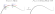
\includegraphics[width=0.9\textwidth]{figs_part2/sec7.5_kinematically_constrained_cosserat_rods/cosserat_rod_to_filament.pdf}
        \caption{(Left) A Cosserat rod, with configuration space $SE(3)$. (Right) A filament, with configuration space in $SE(3)/SO(3) \cong \mathbb{E}^3$.}
        \label{fig:cosserat rod and filament}
\end{figure}

Thus far we have considered the material frame $E$ and the center-line $\mathbf{r}$ as independent degrees of freedom, modelling a rod that can shear and twist in addition to bending and extending. In many applications it suffices to consider pure center-line dynamics where the cross-section does not shear \citep{eloyKinematicsMostEfficient2012, tornbergSimulatingDynamicsInteractions2004, goldsteinNonlinearDynamicsStiff1995, sodaDynamicsStiffChains1973, nordgrenComputationMotionElastic1974, hasimotoSolitonVortexFilament1972}. We shall refer to these systems as \textit{filaments}, and can be seen as a Cosserat rod model with a kinematically constrained material frame. As we will show, kinematic constraints can often be implemented by first identifying an appropriate Lie subgroup $H \subset SE(3)$ such that the homogeneous space $SE(3) / H$ is the kinematically constrained configuration space, and then by making a `gauge choice' $h(u) \in H$ which fixes a parametrisation of $SE(3) / H$. In addition to the filament, we will also consider the case of a \textit{twisting filament}, where the cross-section is allowed to twist around the center-line \citep{powersDynamicsFilamentsMembranes2010, parkerDerivationNonlinearRod1984a, goldsteinViscousNonlinearDynamics1998}.

\subsection{Kinematic constraints and gauge freedoms} \label{sec:Kinematic constraints and gauge freedoms}

The configuration space of a filament can be found by `rotating away' the material frame $E(u)$ at each $u$. Therefore the appropriate Lie subgroup is $H = SO(3)$, and the configuration space is $SE(3) / SO(3) \cong \mathbb{E}^3$, where $\mathbb{E}^3$ is the three-dimensional Euclidean space. Conceptually, that $SE(3)/SO(3)$ represents the configuration space of the filament can be understood by recalling the definition of a homogeneous space. For any Lie group $G$ and Lie subgroup $H \subset G$ then $G/H$ is the set
\begin{equation}
G / H = \{ gH\ |\ g \in G \}
\end{equation}
where $gH = \{ gh\ |\ h \in G \}$ is the left coset. Now consider the case when $G = SE(3)$ and $H = SO(3)$. Let $g_1 = (\mathbf{r}, E_1)$ and $g_2 = (\mathbf{r}, E_2)$ denote two cross-sections that are located at the same point $\mathbf{r}$, but have two different material frames $E_1$ and $E_2$, and furthermore we can trivially identify these as elements $g_1, g_2 \in SE(3)$. As $E_1$ is related to $E_2$ by a rotation in $SO(3)$, we have that $g_1 H = g_2 H$. In other words, in the homogeneous space $SE(3)/SO(3)$, $g_1$ and $g_2$ belong to the same element $g_1 H = g_2 H \in SE(3)/SO(3)$. Therefore, a filament can mathematically be described as a Cosserat rod where we have, for each $u$, identified all material frames $E(u)$ at $\mathbf{r}(u)$ as belonging to the same equivalence~class. See Fig.~\ref{fig:cosserat rod and filament} for an illustration.

Now let $\Phi : W \to SE(3)/SO(3)$ be the spatio-temporal configuration of the filament. As discussed in Sec.~\ref{sec:Sub-manifolds of homogeneous spaces}, we can write $\Phi$ as
\begin{equation} \label{eq:phi and phi tilde}
\Phi = \pi \circ \tilde{\Phi}
\end{equation}
where $\circ$ denotes compositions of maps and $\pi : SE(3) \to SE(3)/SO(3)$ relates elements in $SE(3)$ to elements in the homogeneous space and can be defined as
\begin{equation}
\pi( (\mathbf{r} ; E) ) = \mathbf{r},
\end{equation}
and $\tilde{\Phi} : W \to SE(3)$ is a \textit{framing}, or an \textit{adapted frame field}, of $\Phi$ \citep{clellandFrenetCartanMethod2017}, and is a Lie group-valued function on $W$ that satisfies Eq.~\ref{eq:phi and phi tilde}.

We can map any framing $\tilde{\Phi}$ to a spatio-temporal filament configuration $\Phi$ using Eq.~\ref{eq:phi and phi tilde}. Note however that this map is not injective. Let $h : W \to SO(3)$ be an arbitrary $SO(3)$-valued smooth function and let $\tilde{\Phi}_1 : W \to SE(3)$ and $\tilde{\Phi}_2 : W \to SE(3)$, then if $\tilde{\Phi}_1(t,u) = h(t,u) \tilde{\Phi}_2(t,u)$ maps to the same $\Phi$. Any given choice of $\tilde{\Phi}$ is called a \textit{framing} of $\Phi$ \citep{clellandFrenetCartanMethod2017}. There is thus a \textit{gauge freedom} in the choice of $\tilde{\Phi}$.

In principle, the kinematic and dynamical equations for a Cosserat rod Eq.~\ref{eq:all eoms} apply to the filament as well. We could initialise Eq.~\ref{eq:all eoms} with some $\tilde{\Phi}(u, 0)$ that maps to the true initial condition $\Phi(u, 0)$, then simulate the equations of motion to find $\tilde{\Phi}(t,u)$, and then finally use Eq.~\ref{eq:phi and phi tilde} to find $\Phi(t, u)$. In this case, it is important that all constitutive and body forces and moments only couple to the center-line $\mathbf{r}$, and not the material frame $E$. For example, for conservative constitutive dynamics we could have a potential energy density $\mathcal{U} \propto \kappa^2$, where $\kappa$ is the scalar curvature of the center-line defined in Eq.~\ref{eq:scalar curvature}.

However, the above would mean simulating equations of motion of higher-dimensionality than the system in question, where the extra degrees of freedom (the material frame) are non-physical. In the following we will instead choose a particular \textit{gauge} and form an injective map between $\tilde{\Phi}$ and $\Phi$. In other words, by choosing a gauge we choose a particular prescription for how to frame a given space-curve. Beyond the fact that the resulting dynamics will be defined directly on the lower dimensional $SE(3)/SO(3)$ rather than $SE(3)$, it is also often easier to formulate constitutive dynamics given a particular framing, rather than formulating it in terms of the degrees of freedom of a general Cosserat rod. The programmatic construction of such gauges is better known as the \textit{theory of moving frames} \citep{cartanTheorieGroupesFinis1938, levyReviewElieCartan1935}. We note that the terminological use of `gauge', although well-motivated in this context, is not standard in the theory of moving frames.

All gauge choices are ultimately mathematically equivalent, however some choices are more practically useful than others. Our procedure to construct a gauge will be to write the material frame $E = (\mathbf{e}_1\ \mathbf{e}_2\ \mathbf{e}_3)$ as a function of the center-line $\mathbf{r}$. Thus one-to-one map between $\Phi$ and $\tilde{\Phi}$ is formed. As a first step towards finding an appropriate gauge, we set
\begin{equation} \label{eq:e1 tangent to r}
\mathbf{e}_1 = \frac{\mathbf{r}'}{h}
\end{equation}
where $h = |\mathbf{r}'|$, such that $\mathbf{e}_1$ is a unit-vector tangent to $\mathbf{r}$ at $u$. This means that given $\mathbf{e}_1$ we can write the center-line as
\begin{equation} \label{eq:r from e1}
\mathbf{r}(t, u) = \mathbf{r}(0, t) + \int_0^u h \mathbf{e}_1 du.
\end{equation} 
There is now a remaining $SO(2)$ gauge freedom in specifying the material frame vectors $\mathbf{e}_2$ and $\mathbf{e}_3$. In the gauges found in the literature \citep{bishopThereMoreOne1975a, mansfieldUseRotationMinimizing2019, clellandFrenetCartanMethod2017, carrollImprovingFrenetFrame2013, seligCharacterisationFrenetSerret2013}, most abide Eq.~\ref{eq:e1 tangent to r}, and are thus all related by an $SO(2)$ gauge transformation of $\mathbf{e}_2$ and $\mathbf{e}_3$.

\subsubsection*{The Frenet-Serret gauge}

In the \textit{Frenet-Serret} gauge \citep{frenetCourbesDoubleCourbure1852, serretQuelquesFormulesRelatives1851}, we set
\begin{equation} \label{eq:e2 in frenet-serret}
\mathbf{e}_2 = \frac{\mathbf{e}_1'}{\kappa}
\end{equation}
where $\kappa = |\mathbf{e}_1'|$ is the scalar curvature, such that $\mathbf{e}_2(u)$ is a unit-vector pointing in the direction of the center-line $\mathbf{r}(t,u)$ curves towards at time $t$. Eq.~\ref{eq:e2 in frenet-serret} fully specifies the frame, as $\mathbf{e}_3 = \mathbf{e}_1 \times \mathbf{e}_2$. In this context $\mathbf{e}_1$, $\mathbf{e}_2$ and $\mathbf{e}_3$ are called the tangent, normal and binormal vectors respectively. co

Now recall the equations of motion of $\mathbf{r}$ and $\mathbf{e}_i$ along $u$, given by Eq.~\ref{eq:dr and de}, which we write as
\begin{subequations}
\begin{align}
\mathbf{r}' & = \mathbf{e}_i \theta_i \\
\mathbf{e}_j' & = \mathbf{e}_i \hat{\pi}_{ij}.
\end{align}
\end{subequations}
Since $\mathbf{r}' = h \mathbf{e}_1$ we have that
\begin{equation} \label{eq:theta for filament}
\vec{\theta} = (h\ 0\ 0)^T,
\end{equation}
and as $\mathbf{e}_1' = \kappa \mathbf{e}_2$ we have that $\hat{\pi}_{21} = - \hat{\pi}_{12} = \kappa$ and $\hat{\pi}_{31} = -\hat{\pi}_{13} = 0$. This leaves only one more possible parameter $\hat{\pi}_{23} = -\hat{\pi}_{32}$, to which we assign the scalar parameter $\tau$, known as the \textit{torsion}. We thus have
\begin{equation} \label{eq:pi for filament}
\hat{\pi} = \begin{pmatrix}
0 & - \kappa & 0 \\
\kappa & 0 & - \tau \\
0 & \tau & 0.
\end{pmatrix}
\end{equation}
or, in vector form, $\vec{\pi} = (\tau\ 0\ \kappa)^T$. Finally, we get the \textit{Frenet-Serret equations}
\begin{equation} \label{eq:frennet-serret equations}
\begin{matrix}
\mathbf{e}_1' & = & & \kappa \mathbf{e}_2 & \\
\mathbf{e}_2' & = & - \kappa \mathbf{e}_1 & + & \tau \mathbf{e}_3 & \\
\mathbf{e}_3' & = &  & \tau \mathbf{e}2  &
\end{matrix}
\end{equation}
which together with Eq.~\ref{eq:r from e1} reconstructs the framing $\tilde{\Phi} \cong (\mathbf{r}, E)$, from which get the filament configuration $\Phi \cong \mathbf{r}$.

We see that by choosing a gauge, we have effectively constrained the spatial configuration $X$ to only take values in a subset $V \subset \mathfrak{se}(3)$, where $X = X(h, \kappa, \tau)$ is now parametrised by the three scalars $(h, \kappa, \tau)$ that are functions of space and time. Note that $V$ is not a Lie subalgebra. This constraint establishes an injective mapping between $V$-valued fields $X : W \to V$ and $\mathbb{E}^3$-valued fields $\Phi : W \to \mathbb{E}^3$. In this context $(h, \kappa, \tau)$ are known as the \textit{differential invariants} of the filament, as they uniquely define the filament up to rigid body transformations.

We should stress that in the mathematical literature, the purview of the theory of moving frames are in general space curves (rather than space-time curves). Furthermore, in that context the metric $h$ along the center-line is of little importance (and is usually not referred to as a differential invariant), and thus the arc-length parameterisation is preferred. Eq.~\ref{eq:frennet-serret equations} is therefore more commonly written in terms of arc-length derivatives
\begin{equation} \label{eq:frennet-serret equations arc-length}
\begin{matrix}
\partial_s \mathbf{e}_1 & = & & \tilde{\kappa} \mathbf{e}_2 & \\
\partial_s \mathbf{e}_2 & = & - \tilde{\kappa} \mathbf{e}_1 & + & \tilde{\tau} \mathbf{e}_3 & \\
\partial_s \mathbf{e}_3 & = &  & \tilde{\tau} \mathbf{e}2  &
\end{matrix}
\end{equation}
where $\tilde{\kappa} = h \kappa$ and $\tilde{\tau} = h \tau$ are the scalar curvature and torsion in the arc-length parameterisation.

Intuitively, we can visualise the motion of $(\mathbf{r}, E)$ as a function of $u$, for fixed $t$, in the Frenet-Serret gauge as follows. We can imagine an airplane which is travelling in the direction of $\mathbf{e}_1$ and with the floor of the plane aligned with $\mathbf{e}_3$. Its trajectory traces out a center-line $\mathbf{r}(u)$, at `speed' $h$. The Frenet-Serret frame corresponds to a plane that navigates \textit{pitching} (at a rate $\kappa$) and \textit{rolling} (at a rate $\tau$), but never \textit{yaws}.

We now consider the kinematics along time $t$. The same kinematic equations of motion Eq.~\ref{eq:kinematic equations of motion in the moving frame} for the Cosserat rod still apply. However, substituting $\vec{\theta} = (h\ 0\ 0)^T$ and $\vec{\pi} = (\tau\ 0\ \kappa)^T$ into Eq.~\ref{eq:kinematic equations of motion in the moving frame} we find the following constraints
\begin{subequations} \label{eq:angular velocity in frenet-serret}
\begin{align}
\Omega_1 & = (\Omega_3 \tau - \Omega_2') / \kappa \\
\Omega_2 & = - h^{-1} (D_u \vec{V})_3 \\
\Omega_3 & = h^{-1} (D_u \vec{V})_2.
\end{align}
\end{subequations}
It is intuitive that the angular velocity of the filament, with a cross-section constrained to be aligned with the center-line, is completely determined as a function of the differential invariants and the translational velocity $\vec{V}$. Eq.~\ref{eq:angular velocity in frenet-serret}, together with Eq.~\ref{eq:kinematic equations of motion in the moving frame}, completely specify the kinematics of the filament. Just as we have three scalar parameters $(h, \kappa, \tau)$ that determine the spatial configuration of the filament, the temporal evolution is determined by the three scalars in $\vec{V} = (V_1\ V_2\ V_3)$. Using Eq.~\ref{eq:kinematic equations of motion in the moving frame} and Eq.~\ref{eq:angular velocity in frenet-serret}, we can write the kinematic equations of motion for the filament compactly as
\begin{subequations} \label{eq:filament kinematic equtions of motion}
\begin{align}
\dot{h} & = V_1' - \kappa V_2 \\
\dot{\kappa} & = \Omega_3' + \tau \Omega_2 \\
\dot{\tau} & = \Omega_1' - \kappa \Omega_2 \\
\end{align}
\end{subequations}
where $\vec{\Omega}$ is given by Eq.~\ref{eq:angular velocity in frenet-serret}. The temporal evolution of the filament is thus specified by the velocity field $\vec{V}$ alone.

%\subsubsection{The Bishop gauge}

%The \textit{Bishop} gauge \citep{bishopThereMoreOne1975a, carrollImprovingFrenetFrame2013} is an alternative to the Frenet-Serret frame.

\subsubsection*{The twisting filament}

We can model a filament that can twist around its center-line by keeping the $SO(2)$ gauge freedom of $(\mathbf{e}_2, \mathbf{e}_3)$ and promoting it to a kinematic degree of freedom. The resulting degrees of freedom are then $\vec{\theta} = (h\ 0\ 0)^T$ as before and $\vec{\pi}$ has all three of its components. The resulting constraints on $\vec{\Omega}$ are then
\begin{subequations} \label{eq:angular velocity for twisting filament}
\begin{align}
\Omega_2 & = - h^{-1} (D_u \vec{V})_3 \\
\Omega_3 & = h^{-1} (D_u \vec{V})_2.
\end{align}
\end{subequations}
instead of Eq.~\ref{eq:angular velocity in frenet-serret}. The resulting kinematic equations of motion are thus
\begin{subequations} \label{eq:twisting filament kinematic equtions of motion}
\begin{align}
\dot{h} & = V_1' - \kappa V_2 \\
\dot{\vec{\pi}} & = D_u \vec{\Omega}
\end{align}
\end{subequations}
The temporal evolution of the twisting filament is thus specified by the rate of twist $\Omega_1$ and the velocity field $\vec{V}$.

In our airplane analogy, the twisting filament travels (again, as a function of $u$ for fixed $t$) by rolling (at a rate $\pi_1$), yawing (at a rate $\pi_2$) and pitches (at a rate $\pi_3$).

\subsection{Kinematically constrained dynamics} \label{sec:Kinematically constrained dynamics (cosserat rod)}

The formulation of the dynamics for kinematically constrained rods carries through less programmatically than in the case of the Cosserat rod. In general, extra care must be taken formulating the dynamics when the configuration space is a homogeneous space $G / H$. Issues of under- or over-determination in the equations of motion may arise due to the fact that $\text{dim}(G/H) < \text{dim}(G)$ if $\text{dim}(H) \neq 0$.

\subsubsection*{Filament dynamics}

For a filament, though its configuration space is $SE(3)/SO(3) \cong \mathbb{E}^3$ rather than $SE(3)$ as for the Cosserat rod, $SE(3)$ acts \textit{transitively} on $\mathbb{E}^3$. By which we mean that for any two elements $\mathbf{x}, \mathbf{y} \in \mathbb{E}^3$, there exists an element $g \in SE(3)$ such that $\mathbf{y} = g \mathbf{x}$. As before, we can define a Lagrangian density $\mathcal{L} : SE(3) \times TSE(3) \to \mathbb{R}$, with reduction $\ell : \mathfrak{se}(3) \to \mathbb{R}$, or use the Lagrange-D'Alembert principle as the starting point. The derivation of the dynamics then proceed as before in Sec.~\ref{sec:Cosserat rod dynamics}, and we find the same general equations of motion Eq.~\ref{eq:all eoms}.

However, issues arise as the dimension of the Lie algebra $\text{dim}(\mathfrak{se}(3)) = 6$ is larger than the configuration space $\text{dim}(\mathbb{E}^3) = 3$. This is in principle partially ameliorated by choosing a gauge, such as the Frenet-Serret gauge, but if this is done naively then the resulting equations of motion are untenable. Consider the dynamical equations of motion that would result if we consider a filament with the Frenet-Serret frame, starting from the Lagrange-D'Alembert principle Eq.~\ref{eq:lagrange-dalembert for non-monogenic constitutive forces and body forces}. As before, we let $S = \frac{\partial \mathcal{K}}{\partial N}$, where the reduced kinetic energy $\mathcal{K}$ of the Cosserat rod was derived in Eq.~\ref{eq:reduced kinetic energy} and we repeat it here
\begin{equation}
\mathcal{K}(N)  = \frac{1}{2} \rho_0 |\vec{V}|^2 +  \frac{1}{2} \vec{\Omega}^T \mathbb{I} \vec{\Omega}.
\end{equation}
Consider now, in particular, the moment balance equation for the filament
\begin{equation} \label{eq:moment balance filament wrong}
D_t \vec{L} = D_u \vec{M} + \vec{\theta} \times \vec{F} + \vec{m},
\end{equation}
where $\vec{L} = \mathbb{I} \vec{\Omega}$. Due to Eq.~\ref{eq:angular velocity in frenet-serret}, $\vec{\Omega}$ is not an independent degree of freedom, but a function of $\vec{V}$ and the differential invariants. Therefore Eq.~\ref{eq:moment balance filament wrong} over-determines the system, and is in general an intractable constraint.

To address this issue, we first note that it stems from the particular method by which we have parametrised the filament. In the fixed frame, the dynamics of the filament can be unambiguously written as
\begin{equation} \label{eq:fixed frame filament dynamics}
\rho_0 \ddot{\mathbf{r}} = \mathbf{F}' + \mathbf{f}
\end{equation}
where we used $\mathbf{P} = \rho_0 \dot{\mathbf{r}}$, which can be seen as the $1$-dimensional analogue of the Cauchy momentum equation in the Lagrangian point-of-view, where $\mathbf{F}$ would correspond to the \textit{first Piola-Kirchhoff stress tensor} in continuum dynamics.

In the geometric formulation presented here, we parametrise the filament in terms of its intrinsic geometry $\kappa$ and $\tau$, which corresponds to a given framing, rather than its center-line $\mathbf{r}(t,u)$ as in Eq.~\ref{eq:fixed frame filament dynamics}. This means that we must consider how the forces on the filament corresponds to moments on the moving frame $(\mathbf{e}_1, \mathbf{e}_2, \mathbf{e}_3)$. However, as the filament is ultimately described as a center-line, the model does not accommodate the angular momentum of its frame as an independent degree of freedom. In the literature the issue of Eq.~\ref{eq:moment balance filament wrong} is avoided by taking the overdamped limit modelling a filament immersed in a highly viscous fluid \citep{eloyKinematicsMostEfficient2012, tornbergSimulatingDynamicsInteractions2004, goldsteinNonlinearDynamicsStiff1995, sodaDynamicsStiffChains1973, nordgrenComputationMotionElastic1974, hasimotoSolitonVortexFilament1972, powersDynamicsFilamentsMembranes2010, goldsteinViscousNonlinearDynamics1998}, or by considering filament statics \citep{parkerDerivationNonlinearRod1984a}. Here, we avoid this limit and present a derivation of inertial filament dynamics.

Let $\mathcal{K}(N)  = \frac{1}{2} \rho_0 |\vec{V}|^2$, so that we get $S = \{ \vec{P} ; \vec{0} \}$ where $\vec{P} = \rho_0 \vec{V}$, therefore implicitly assuming the angular momentum of the filament to be negligible. The moment balance equation then becomes
\begin{equation} \label{eq:moment balance filament}
0 = D_u \vec{M} + \vec{\theta} \times \vec{F} + \vec{m}.
\end{equation}
To find self-consistent constitutive dynamics, we consider moment balance in the absence of external moments $\vec{m} = 0$, to find
\begin{subequations} \label{eq:filament force constraints}
\begin{align}
0 &  = (D_u \vec{M})_1 \\
F_2 & = h^{-1} (D_u \vec{M})_3 \\
F_3 & = - h^{-1} (D_u \vec{M})_2.
\end{align}
\end{subequations}
Thus we see that combined we can only independently specify three of the six force and moment components in total. The kinematic and dynamical equations of motion for the filament are thus
\begin{subequations} \label{eq:filament dynamic equtions of motion}
\begin{align}
\dot{h} & = V_1' - \kappa V_2 \\
\dot{\kappa} & = \Omega_3' + \tau \Omega_2 \\
\dot{\tau} & = \Omega_1' - \kappa \Omega_2 \\
D_t \vec{P} & = D_u \vec{F} + \vec{f},
\end{align}
\end{subequations}
where the material derivatives are computed as before, using $\vec{\pi} = (\tau\ 0\ \kappa)$ and $\vec{\Omega}$ given by Eq.~\ref{eq:angular velocity in frenet-serret}, and where the force must obey the conditions Eq.~\ref{eq:filament force constraints}. We note that $\vec{M}$ does not appear explicitly in the dynamics, and we can indeed in theory write down the three arbitrary constitutive force components $\vec{F}$, which would induce a moment via Eq.~\ref{eq:filament force constraints} that has no impact on the dynamics. This is however not how the constitutive forces and moments are defined in practice, as we will now show.

We now move on to treat conservative constitutive dynamics. As discussed in \citep{levyReviewElieCartan1935}, when the Lie algebra, that acts transitively on the configuration space, is of a higher dimension than the configuration space the resulting Lagrangian dynamics (i.e. conservative dynamics) is under-determined. For a Cosserat rod we have $Q = \frac{\partial \mathcal{U}}{\partial X} = \{ \vec{F} ; \vec{M} \}$ which results in Eq.~\ref{eq:F_i and M_i from U}. In contrast, as $\vec{\theta} = (h\ 0\ 0)^T$ and $\vec{\pi} = (\tau\ 0\ \kappa)^T$ for a filament, the only components that are determined for a general constitutive $\mathcal{U}$ are
\begin{subequations} \label{eq:F1, M2 and M3 for filament}
\begin{align}
F_1 & =  \frac{\partial \mathcal{U}}{\partial h} \\
M_1 & =  \frac{\partial \mathcal{U}}{\partial \tau} \\
M_3 & =  \frac{\partial \mathcal{U}}{\partial \kappa} 
\end{align}
\end{subequations}
leaving $M_2$, $F_2$ and $F_3$ undetermined by $\mathcal{U}$. However we see that by having chosen a gauge, these force and moment components are given by moment balance Eq.~\ref{eq:filament force constraints}. The conservative constitutive forces and moments on a filament are thus determined by Eq.~\ref{eq:F1, M2 and M3 for filament} and Eq.~\ref{eq:filament force constraints} together. Note that it was necessary to let $M_1$, $F_2$ and $F_3$ be undetermined by $\mathcal{U}$, rather than setting $M_1 = F_2 = F_3 = 0$, which would conflict with moment balance. The above is consistent with the force and moment balance equations found for the filament in the overdamped setting \citep{powersDynamicsFilamentsMembranes2010} and in statics \citep{parkerDerivationNonlinearRod1984a}.

It is standard for filament dynamics to associate an energetic cost to the square of the curvature and extension $\mathcal{U} = \frac{1}{2} \epsilon \kappa^2$.  From Eq.~\ref{eq:F1, M2 and M3 for filament} and Eq.~\ref{eq:filament force constraints} we then find, expressed in a non-moving frame
\begin{equation} \label{eq:bernoulli moment for filament}
\mathbf{M} = \epsilon \kappa \mathbf{e}_3
\end{equation}
where $\epsilon$ is the bending stiffness. Eq.~\ref{eq:bernoulli moment for filament} agree with classical Bernoulli-Euler beam theory \citep{ powersDynamicsFilamentsMembranes2010, sodaDynamicsStiffChains1973, nordgrenComputationMotionElastic1974}. Note that as the notion of torsion $\tau$ appears from the gauge choice, rather than representing a physical property of the filament, a $\tau^2$ term is usually not included in $\mathcal{U}$. Therefore $M_1 = M_2 = 0$ for a filament in the Frenet-Serret frame in practice.

In the overdamped limit, the results of Sec.~\ref{sec:Dissipative and overdamped dynamics} and Eq.~\ref{eq:overdamped equations of motion in moving frame} applies as before, under the constraints Eq.~\ref{eq:theta for filament} and Eq.~\ref{eq:pi for filament}, Eq.~\ref{eq:angular velocity in frenet-serret} and Eq.~\ref{eq:filament force constraints}. Setting $\vec{f} = - \gamma_T \vec{V}$ we get
\begin{subequations} \label{eq:filament overdamped equtions of motion}
\begin{align}
\dot{h} & = V_1' - \kappa V_2 \\
\dot{\kappa} & = \Omega_3' + \tau \Omega_2 \\
\dot{\tau} & = \Omega_1' - \kappa \Omega_2 \\
\vec{V} & = \mu_T D_u \vec{F},
\end{align}
\end{subequations}
where $\mu_T = \gamma_T^{-1}$.

\subsubsection*{Twisting filament dynamics}

For a twisting filament, the angular velocity component $\Omega_1$ is now a dynamic degree of freedom, and we therefore permit angular momentum along the tangential direction. We assume the principal axes of the moment of inertia $\mathbb{I}$ coincide with the moving frame $\mathbf{e}_i,\ i=1,2,3$, and that the angular momentum is negligible along the normal and binormal directions, setting $\vec{L} = ( \mathbb{I}^{(1)} \Omega_1\ 0\ 0 )^T$, where $\mathbb{I}^{(1)}$ is the eigenvalue of $\mathbb{I}$ along $\mathbf{e}_1$. The resulting kinematic and dynamical equations of motion are
\begin{subequations} \label{eq:twisting filament dynamic equtions of motion}
\begin{align}
\dot{h} & = V_1' - \kappa V_2 \\
\dot{\pi} & = D_u \vec{\Omega} \\
D_t \vec{P} & = D_u \vec{F} + \vec{f} \\
\mathbb{I}^{(1)} \dot{\Omega}_1 & = (D_u \vec{M})_1 + m_1
\end{align}
\end{subequations}
where the constraints on the force are
\begin{subequations} \label{eq:twisting filament force constraints}
\begin{align}
F_2 & = h^{-1} (D_u \vec{M})_3 \\
F_3 & = - h^{-1} (D_u \vec{M})_2,
\end{align}
\end{subequations}
which should be compared with Eq.~\ref{eq:filament dynamic equtions of motion} and Eq.~\ref{eq:filament force constraints}. For conservative constitutive we now have the relations
\begin{subequations} \label{eq:F1 and M for twisting filament}
\begin{align}
F_1 & =  \frac{\partial \mathcal{U}}{\partial h} \\
M_i & =  \frac{\partial \mathcal{U}}{\partial \pi_i}.
\end{align}
\end{subequations}


\begin{comment}
\subsubsection*{Inextensible Cosserat rods and filaments}

A Cosserat rod is \textit{inextensible} if it satisfies the kinematic constraint $\dot{h} = 0$. 


We will now consider the case of an inextensible Cosserat rod in the
overdamped limit, under the influence of a constitutive force $\vec{F}$.
For an inextensible rod, the tangential component of the force, tangent
to the center-line $\mathbf{r}$, is a constraining tension that enforces $\mathbf{r}'\cdot\mathbf{r}'=\boldsymbol{\theta}\cdot\boldsymbol{\theta}=1$.
Using Eq. \ref{eq:theta eom} and Eq. \ref{eq:V overdamped} we find
that the force must satisfy

\begin{equation}
\vec{\theta}^{T}D_{u}^{2}\vec{F}=0.\label{eq:Ft constraint}
\end{equation}
Equation \ref{eq:Ft constraint} should be seen as a constraint on
$F_{1}$. Though in practice it is often more covenient to consider
a tension force $\vec{T}$ separate from the rest of the constitutive
dynamics $\vec{F}$, such that the total force on the filament be
$\tilde{\vec{F}}=\vec{F}+\vec{T}$. As a tensional force must act
tangentially along the filament, we must have $\vec{T}\propto\vec{\theta}$,
and so we write $\vec{T}=T\vec{\theta}$. The tension force will enforce
the condition $\partial_{t}(\vec{\theta}^{T}\vec{\theta})=2\dot{\vec{\theta}}^{T}\vec{\theta}=0$.
From Eq. \ref{eq:Ft constraint} we find
\begin{equation}
\vec{\theta}^{T}\partial_{u}^{2}(\vec{F}+T\vec{\theta})=0\label{eq:tension}
\end{equation}
which is a non-linear 2nd order ODE for $T$. Note that using Eq.
\ref{eq:tension} renders the component of the force tangent to the
center-line $F_{\theta}=\boldsymbol{\theta}\cdot\mathbf{F}$ redundant
and has no effect on the system. Using $\theta_{i}\theta_{i}=1$ and
$\partial_{u}(\theta_{i}\theta_{i})=2\theta_{i}'\theta_{i}=0$, Eq.
\ref{eq:tension} simplifes to
\begin{equation}
(\partial_{u}^{2}-H)T=-\vec{\theta}^{T}D_{u}^{2}\vec{F}\label{eq:tension eq}
\end{equation}
where $H=-\theta_{i}\theta_{i}''+2\theta_{i}\hat{\pi}_{ij}\theta_{j}'-\theta_{i}\hat{\pi}_{ij}\hat{\pi}_{jk}\theta_{k}$.
In numerical experiments Eq. \ref{eq:tension} would have to be solved
at each time-step to compute the tensional force.

For a special Cosserat rod or filament the constraint simplifies to
$\theta_{1}=h=1$, implying $\dot{h}=0$. Furthermore, $F_{1}=F_{\theta}$
is now tangent to the center-line. The equation for $T$ simplifies
to
\begin{equation}
(\partial_{s}^{2}-(\pi_{2}^{2}+\pi_{3}^{2}))T=-\nabla_{u}^{2}F_{1}
\end{equation}
and $\mathbf{T}=T\mathbf{e}_{1}$. Note that the tangential component
of the force $F_{1}$ is redundant here, and can be safely set to
zero.
\end{comment}


\section{The hyperelastic Cosserat rod model} \label{sec:The hyperelastic Cosserat rod model}

In many applications the conservative part of the constitutive dynamics arise from a potential of the form Eq.~\ref{eq:U quadratic form} \citep{NonlinearProblemsElasticity2005, wangOptimalControlSoft2021a, gargSlenderBodyTheory2022, tillRealtimeDynamicsSoft2019}, where the potential $\mathcal{U}$ is a quadratic form in $X$, with coefficients given by the symmetric and positive-definite stiffness matrix $\mathsf{K} \in \mathbb{R}^{6 \times 6}$. Here we derive the form of $\mathsf{K}$ from first principles, given constitutive assumptions on the material that the rod is composed of. Specifically, we model the Cosserat rod as a slender tube of hyper-elastic \textit{Saint Venant-Kirchoff} material \cite{basarNonlinearContinuumMechanics2013}, but the derivation carries through regardless of what constitutive assumption.

We consider a straight rod $\mathscr{M}=\mathscr{D} \times [0,L_{0}]$ at rest, where $\mathscr{D}$ is a disc of arbitrary shape, and $L_{0}$ is the length of the rod.
As before, $\mathbf{X}$ is the material coordinate on $\mathscr{M}$, and we align $X_{1}\in[0,L_{0}]$ along the length of the rod, and $(X_{2},X_{3})\in\mathscr{D}$. We will use $u = X_1$ and $X_1$ interchangeably. Deformations of $\mathscr{M}$ are given by $\mathbf{x}(\mathbf{X})$, which we will refer to as the \textit{deformed coordinate}. The material and deformed coordinates can be related as
\begin{equation}
d\mathbf{x}= \mathcal{P} d\mathbf{X}
\end{equation}
where $\mathcal{P} =\frac{\partial\mathbf{x}}{\partial\mathbf{X}}$ is here the \emph{deformation
gradient tensor}, and we write its components in the moving frame $\mathcal{P}_{ij} = \mathbf{e}_i \cdot \left( \frac{\partial\mathbf{x}}{\partial\mathbf{X}} \mathbf{e}_j \right)$. Following \citep{landauTheoryElasticityVolume1986}, we consider
the change in infinitesimal distances between two material points $\mathbf{X}_{1}$ and $\mathbf{X}_{2}$ in the rod after a deformation. In the undeformed
state, the distance between $\mathbf{X}_{1}$ and $\mathbf{X}_{2}$
is $d\ell^{2}=|d\mathbf{X}|^{2}$. After deformation we have
\begin{equation} \label{eq:deformation}
\begin{aligned}d\ell'^{2}=|d\mathbf{x}|^{2} & =(Pd\mathbf{X})^{T}(\mathcal{P} d\mathbf{X})\\
 & =d\mathbf{X}^{T} \mathcal{P}^{T} \mathcal{P} d\mathbf{X}\\
 & =d\ell^{2}+2d\mathbf{X}^{T}Ed\mathbf{X}\\
 & =d\mathbf{X}^{T}(I+2E)d\mathbf{X}
\end{aligned}
\end{equation}
where
\begin{equation} \label{eq:Lagrangian strain tensor}
E=\frac{1}{2}\left(\frac{\partial\mathbf{u}}{\partial\mathbf{X}}+\left(\frac{\partial\mathbf{u}}{\partial\mathbf{X}}\right)^{T}+\left(\frac{\partial\mathbf{u}}{\partial\mathbf{X}}\right)^{T}\frac{\partial\mathbf{u}}{\partial\mathbf{X}}\right) 
\end{equation}
is the \emph{Lagrangian strain tensor} and $\mathbf{u}(\mathbf{X})=\mathbf{x}-\mathbf{X}$ is the \emph{deformation vector}. For small deformations, we can approximate
Eq. \ref{eq:deformation assumption} as $E\approx\frac{1}{2}\left(\frac{\partial\mathbf{u}}{\partial\mathbf{X}}+\left(\frac{\partial\mathbf{u}}{\partial\mathbf{X}}\right)^{T}\right)$,
in which case we can express it as
\begin{equation} \label{eq:approximated E}
E=\frac{1}{2}(\mathcal{P}+\mathcal{P}^{T}-2 \mathbbm{1}).
\end{equation}
The Lagrangian strain tensor can be seen as giving the relative deformations
along the principle axes of a material, where the latter are defined as the eigenvectors $E$. The elastic energy density of the material in a deformed state is a function of $E$, and we assume it to be a quadratic form
\begin{equation} \label{eq:general Kirchoff W}
W(E) = \frac{1}{2} C_{ijkl} E_{ij} E_{kl}
\end{equation}
where $C_{ijkl}$ is a fourth-order tensor of elastic constants, which is known as the Saint Venant-Kirchoff constitutive assumption \cite{basarNonlinearContinuumMechanics2013}, and materials that are well-approximated under this assumption are known as \textit{Saint Venant-Kirchoff materials}. If we assume that $C$ is isotropic, in which case it has the form
\begin{equation}
C_{ijkl} = \lambda \delta_{ij} \delta_{kl} + \mu_1 \delta_{ik} \delta_{jl} + \mu_2 \delta_{il} \delta_{jk}
\end{equation}
then Eq.~\ref{eq:general Kirchoff W} can be shown to reduce to
\begin{equation} \label{eq:elastic energy per volume}
W(E)=\mu\text{Tr}(E^{2})+\frac{\lambda}{2}\text{Tr}(E)^{2}
\end{equation}
where $\lambda$ and $\mu = \mu_1 + \mu_2$ are known as the \textit{Lamé constants}.

We will now proceed to derive the potential energy per unit material length of a Cosserat rod under the constitutive assumption of Eq.~\ref{eq:elastic energy per volume}. We impose the kinematic assumption Eq.~\ref{eq:cosserat rod kinematic assumption}, which we write again here as
\begin{equation}
\mathbf{x}(\mathbf{X})=\mathbf{r}(X_{1})+\mathbf{e}_{\xi}X_{\xi},\ \xi=2,3\label{eq:deformation assumption}
\end{equation}
which constrains deformations to preserve the area and shape of the cross-section at each $X_{1}$. Since
\begin{equation}
\frac{\partial \mathbf{x}}{\partial X_1} = \theta_i \mathbf{e}_i + \mathbf{e}_i \hat{\pi}_{i \gamma} X_\gamma, \quad \gamma = 2,3
\end{equation}
where we used Eq.~\ref{eq:dr and de}, we have
\begin{equation} \label{eq:P cosserat rod}
\begin{aligned}
\mathcal{P}_{i1} & =\theta_{i}+ \pi_{i \gamma} X_{\gamma}\\
\mathcal{P}_{i\gamma} & =\delta_{i\gamma}.
\end{aligned}
\end{equation}
The Lagrangian strain tensor $E$ can then be computed using Eq.~\ref{eq:approximated E}, and since Eq.~\ref{eq:P cosserat rod} is expressed entirely in terms of $X = \{ \vec{\theta} ; \vec{\pi} \}$, we can express the energy volume density $W$ as a function of $X$ as well. To find the energy density per unit-length $\mathcal{U}(\vec{\theta}, \vec{\pi})$ of the rod, we must integrate out the cross-section
\begin{equation}
\mathcal{U}(\vec{\theta}, \vec{\pi})=\int_{\mathscr{D}}W(E)dX_{2}dX_{3}.
\end{equation}
For simplicity, we assume a circular cross-section, for which we have that
\begin{equation} \label{eq:cross section integrals}
\begin{aligned}\int_{\mathscr{D}}dA & =\pi R^{2}\\
\int_{\mathscr{D}}X_{\alpha}dA & =0\\
\int_{\mathscr{D}}X_{\alpha}X_{\beta}dA & =\frac{\pi R^{4}}{4}\delta_{\alpha\beta}\\
\int_{\mathscr{D}}X_{\alpha}X_{\beta}X_{\gamma}dA & =0\\
\int_{\mathscr{D}}X_{\alpha}X_{\beta}X_{\gamma}X_{\delta}dA & =\begin{cases}
\frac{\pi R^{6}}{8}, & \alpha=\beta=\gamma=\delta\\
\frac{\pi R^{6}}{24}, & \alpha=\beta\text{ and }\gamma=\delta\\
\frac{\pi R^{6}}{24}, & \alpha=\gamma\text{ and }\gamma=\beta
\end{cases}
\end{aligned}
{U}
\end{equation}
where $\alpha,\beta,\gamma,\delta=2,3$ and $R$ is the radius of
the rod. From Eq.~\ref{eq:cross section integrals}, Eq.~\ref{eq:cross section integrals}, Eq.~\ref{eq:approximated E} and Eq.~\ref{eq:elastic energy per volume}, the potential energy per unit material length evaluates to
\begin{equation} \label{eq:hyperelastic cosserat rod circular cross-section}
\mathcal{U}(\vec{\theta}, \vec{\pi})=\frac{k_{1}}{2}(\theta_{1}-1)^{2}+\frac{k_2}{2}(\theta_{2}^{2}+\theta_{3}^{2})+\frac{\epsilon_1}{2}\hat{\pi}_{1}^{2}+\frac{\epsilon_2}{2}(\hat{\pi}_{2}^{2}+\hat{\pi}_{3}^{3})
\end{equation}
where $k_1=\pi R^{2}(\lambda+2\mu)$, $k_2=\frac{\pi R^{2}}{2}\lambda$, $\epsilon_1=\frac{\pi R^{4}}{4}\lambda$ and $\epsilon_2=\frac{\pi R^{4}}{4}(\lambda+2\mu)$. Equation \ref{eq:hyperelastic cosserat rod circular cross-section} is consistent with the is consistent with the quadratic Cosserat free energies found in the literature \citep{giusteriSimulationViscoelasticCosserat2021, caoNonlinearDynamicsElastic2008, rubinCosseratRods2000}. For a non-circular cross-section we will in general have a potential energy of the form
\begin{equation} \label{eq:general U for hyperelastic rod}
\mathcal{U}(\vec{\theta}, \vec{\pi})=\frac{k_1}{2}(\theta_{1}-1)^{2}+\frac{k_{2}}{2}\theta_{2}^{2}+\frac{k_{3}}{2}\theta_{3}^{2}+\frac{\epsilon_1}{2}\hat{\pi}_{1}^{2}+\frac{\epsilon_{2}}{2}\hat{\pi}_{2}^{2}+\frac{\epsilon_{3}}{2}\hat{\pi}_{2}^{2}.
\end{equation}
We can interpret the form of the potential energy by recalling how $\vec{\theta}$ and $\vec{\pi}$ encodes the various kinematic deformations of the Cosserat rod, described in Sec.~\ref{sec:deformation types}. The first three terms in Eq.~\ref{eq:general U for hyperelastic rod} penalises both shearing of the material frame, as well as extension of the center-line. The $\pi_1$ term penalises twisting of the material frame along $\mathbf{e}_1$, and $\pi_2$ and $\pi_3$ penalises the rotation of the material frame along $\mathbf{e}_2$ and $\mathbf{e}_3$ respectively.

The stiffness matrix of a hyper-elastic Cosserat rod can thus be written as
\begin{equation}
\mathsf{K} = \begin{pmatrix}
K^{(1)} & 0_{3 \times 3} \\
0_{3 \times 3} & K^{(2)}
\end{pmatrix}
\end{equation}
where $K^{(1)} = \text{diag} \left\{ k_1, k_2, k_3 \right\}$ and $K^{(2)} = \text{diag} \left\{ \epsilon_1, \epsilon_2, \epsilon_3 \right\}$, with rest state
\begin{subequations}
\begin{align}
\vec{\theta}_0 & = (1\ 0\ 0)^T \\
\vec{\pi}_0 & = (0\ 0\ 0)^T.
\end{align}
\end{subequations}
The resulting constitutive force and moments are
\begin{subequations}
\begin{align}
\vec{F} & = \frac{\partial \mathcal{U}}{\partial \vec{\theta}} = K^{(1)} (\vec{\theta} - \vec{\theta}_0) \\
\vec{M} & = \frac{\partial \mathcal{U}}{\partial \vec{\pi}} = K^{(2)} \vec{\pi}.
\end{align}
\end{subequations}
We see that in this constitutive model, the force $\vec{F}$ acts on the center-line such as to align with its material frame. In other words, if the material frame is shearing, then the center-line will bend such as to be tangent to $\mathbf{e}_1$. If the material frame is rotating along $u$, which corresponds to a non-zero $\vec{\pi}$, then the moment $\vec{M}$ acts so as to render it non-rotating.  We thus see that a shearing material frame \textit{induces} bend. This effect happens despite the fact that $\vec{\theta}$ and $\vec{\pi}$ do not couple in $\mathcal{U}$, which inherently due to the geometric non-linearities in the kinematics of the Cosserat rod. Conversely, a bending center-line which is aligned with the material frame will induce shear. Note that there is no direct energetic cost for the bending of the center-line itself (as $\mathcal{U}$ is not a function of the scalar curvature $\kappa$), however the energetic cost of shearing, combined with the energetic cost of a rotating material frame, conspire together so as to straighten segments of the rod that bend.

\section{Dissipative and overdamped dynamics} \label{sec:Dissipative and overdamped dynamics}

Equation \ref{eq:dynamics in terms of V and L with body forces} allows us to model general dissipative dynamics. We consider the case of a Cosserat rod that suffers both internal and external friction
\begin{subequations} 
\begin{align}
\dot{X} & = (\partial_u + \text{ad}_N) X \label{eq:kinematics with dissipation} \\
\left(\partial_t - \text{ad}_N^* \right) S & = \left(\partial_u - \text{ad}_X^* \right) Q - \mathsf{H} \dot{X} - \mathsf{G} N \label{eq:dynamics with dissipation} \\
Q & = 0, \quad u = 0, L_0, 
\end{align}
\end{subequations}
where we have set $T = - \mathsf{H} \dot{X} - \mathsf{G} N$, and where $\mathsf{H}$ and $\mathsf{G}$ are positive-definite matrices of damping coefficients of the internal and external friction respectively. Note that $\mathsf{H} \dot{X}$ in Eq.~\ref{eq:dynamics with dissipation} is evaluated by substituting in Eq.~\ref{eq:kinematics with dissipation}. If let the frictional matrices be block-diagonal in the translational and angular components as
\begin{subequations} 
\begin{align}
\mathsf{H} & = \begin{pmatrix}
	\gamma^\text{in}_T & 0_{3 \times 3} \\
	0_{3 \times 3} & \gamma^\text{in}_R
\end{pmatrix} \\ 
\mathsf{G} & = \begin{pmatrix}
	\gamma_T & 0_{3 \times 3} \\
	0_{3 \times 3} & \gamma_R
\end{pmatrix}
\end{align}
\end{subequations}
where $\gamma^\text{in}_T$, $\gamma^\text{in}_R$, $\gamma_T$ and $\gamma_R$ are positive-definite $3 \times 3$-matrices, we can write the equations of motion as
\begin{subequations} 
\begin{align}
D_t \vec{\theta} & = D_u \vec{V} \\
\partial_t \vec{\pi} & = D_u \vec{\Omega} \\
D_t \vec{P} & = D_u \vec{F} - \gamma^\text{in}_T \dot{\vec{\theta}} - \gamma_T \vec{V} \\
D_t \vec{L} & = D_u \vec{M} + \vec{\theta} \times \vec{F}  - \gamma^\text{in}_R \dot{\vec{\pi}} - \gamma_R \vec{\Omega}
\end{align}
\end{subequations}
where again $\gamma^\text{in}_T \dot{\vec{\theta}}$ and $\gamma^\text{in}_T \dot{\vec{\pi}}$ can be evaluated using the kinematic equations of motion, and $\vec{F} = \vec{M} = 0,\ u= 0,L_0$.

We can consider a limit where the dissipative forces dominate over the inertial forces (which correspond to the left-hand side of Eq.~\ref{eq:dynamics with dissipation}). In this limit, we set $S \approx 0$, or equivalently $\vec{P} \approx 0$ and $\vec{L} = \mathbb{I} \vec{\Omega} \approx 0$. The resulting equations are \textit{overdamped} equations of motion
\begin{subequations} 
\begin{align}
\dot{X} & = (\partial_u + \text{ad}_X ) N \label{eq:overdamped kinematics} \\
\mathsf{G} N & = \left( \partial_u - \text{ad}_X^* \right) Q + \mathsf{H} \dot{X} \label{eq:overdamped dynamics} \\
Q & = 0, \quad u = 0, L_0.
\end{align}
\end{subequations}
where we must solve for $N$ in Eq.~\ref{eq:overdamped dynamics} to compute Eq.~\ref{eq:overdamped kinematics}. In terms of the translational and angular velocities, the equations of motion are
\begin{subequations} \label{eq:overdamped equations of motion in moving frame}
\begin{align}
D_t \vec{\theta} & = D_u \vec{V} \\
\partial_t \vec{\pi} & = D_u \vec{\Omega} \\
\gamma_T \vec{V} & = D_u \vec{F} - \gamma^\text{in}_T \dot{\vec{\theta}}  \\
\gamma_R \vec{\Omega} & = D_u \vec{M} + \vec{\theta} \times \vec{F}  - \gamma^\text{in}_R \dot{\vec{\pi}}
\end{align}
\end{subequations}
where again we must solve for $\vec{V}$ and $\vec{\Omega}$ in the latter two equations and substitute them into the kinematic equations of motion. We note that the overdamped equations of motion are first-order in time $t$ and second-order in space $u$ (as opposed to first-order in the underdamped case). Furthermore, the only degree of freedom is here $X = \{ \vec{\theta} ; \vec{\Omega} \}$, and so the dynamics are $6$-dimensional as opposed to $12$-dimensional in the underdamped case.

The presence of the internal friction $\mathsf{H} \dot{X}$ significantly complicates the evaluation of the overdamped dynamics. Substituting Eq.~\ref{eq:overdamped kinematics} into Eq.~\ref{eq:overdamped dynamics} we get a self-consistency relation for $N$
\begin{equation}
\mathsf{G} N = \left( \partial_u - \text{ad}_X^* \right) Q + \mathsf{H} (\partial_u + \text{ad}_X ) N
\end{equation}
and formally we can write $N$ as
\begin{equation}
N = \mathscr{A}^{-1} \left( \partial_u - \text{ad}_X^* \right) Q
\end{equation}
where $\mathscr{A} = \mathsf{G} - \mathsf{H} (\partial_u + \text{ad}_X)$. In simulations, which invariably employ some discretisation scheme, $\mathscr{A}$ becomes a matrix that can be inverted numerically. If, however, we neglect internal dissipation we have $N = \mathsf{G}^{-1} \left( \partial_u - \text{ad}_X^* \right) Q$, and we can write the equations of motion in a compact form as
\begin{equation}
\dot{X}  = (\partial_u + \text{ad}_X ) \left[ \mathsf{G}^{-1} \left( \partial_u - \text{ad}_X^* \right) Q \right]
\end{equation}
or
\begin{subequations} 
\begin{align}
D_t \vec{\theta} & = D_u \left[ \mu_T D_u \vec{F} \right] \\
\partial_t \vec{\pi} & = D_u \left[ \mu_R  D_u \vec{M} \right] 
\end{align}
\end{subequations}
where $\mu_{T,R} = \gamma_{T,R}^{-1}$, which would be the overdamped equations of motion of a Cosserat rod immersed in a viscous medium. 


%%%% Ideas and notes:
 
% - In general $\mathcal{F}_0$ can be dependet on time and space, which would be the way to have a non-straight reference rod.

% - It would be good to show that the dynamics of a filament with a certain potential $U(\kappa)$ has the same dynamics as a Cosserat rod with the same potential.


\chapter{Geometric continuum mechanics on Lie group- and homogeneous configuration spaces} \label{ch:Geometric continuum mechanics on homogeneous configuration spaces}

In Ch.~\ref{ch:Cosserat rods}, we derived the kinematic and dynamical equations of motion of the Cosserat rod and filament, systems in one material dimension with configuration space $SE(3)$ and $SE(3)/SO(3)$ respectively. In the subsequent section we provide a generalisation of Ch.~\ref{ch:Cosserat rods} to systems with general material bases spaces and homogeneous configuration spaces. We call this the \textit{geometrisation programme}. Mathematically, the geometrisation programme can be seen as a general field theory of Lie group- or homogeneous space-valued fields defined over topological manifolds. The derivations of the results are provided in Sec.~\ref{sec:Geometric kinematics} and Sec.~\ref{sec:Geometric dynamics}. 

We have separated the exposition of the results and their derivation, as the latter require a level of mathematical abstraction not necessary in the presentation of the geometrisation programme itself. The primary mathematical challenge stems from allowing arbitrary topologies in the material base space, which entails that it longer admits a global set of coordinates. An example of such a system would be a closed surface, like the membrane of a cell. This necessitated further geometrical abstraction that was not required in the case of the Cosserat rod. 

In Sec.~\ref{sec:geometrisation applications} we use the geometrisation programme to derive the equations of motion for a set of example systems. This section is called `\text{Applications}', meant to be understood in the sense that our general geometric framework is \emph{applied} to derive the kinematic and dynamic theories of the given example systems. When these systems are well-established in the literature, we show that our framework recovers the correct equations of motion. Finally, in Sec.~\ref{sec:geometrisation discussion} we conclude with a summary and discussion on the geometrisation programme.

\section{The geometrisation programme} \label{sec:The geometrisation programme}

\begin{figure}[t]
\centering
        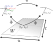
\includegraphics[width=0.8\textwidth]{figs_part2/ch8_geometrisation/cosserat_geometrisation.pdf}
        \caption{The relation between the spatio-temporal configuration $\Phi$ and the adapted frame field $\tilde{\Phi}$ of a filament. In the top-left and top-right we show the mapping of $(t_p, u_p)$, a point in the kinematic base space $W$, to $\tilde{\Phi}(t_p, u_p)$ and $\Phi(t_p, u_p)$, which are related by the projection map $\pi$.}\label{fig:cosserat rod geometrisation illustration}
\end{figure}

Here we generalise the results of Sec.~\ref{sec:Geometric Cosserat rod mechanics} to systems with an arbitrary material base space and homogeneous configuration space. To aid understanding it will be helpful to reintroduce some nomenclature, and to relate and contextualise the mathematical formulation of the Cosserat rod and the filament to the general systems that we describe in what follows. This preamble will thus serve as a brief overview of the results given in the subsequent subsections.

The \textit{material base space} of an open Cosserat rod is the manifold $M = [0, L_0]$, and its \textit{kinematic configuration space} is the Lie group $SE(3)$. The \textit{spatio-temporal configuration} of the Cosserat rod is a map $\Phi : W \to SE(3)$, where $W = [0,T] \times M$ is the \textit{kinematic base space} and $[0,T]$ the time domain. In Sec.~\ref{sec:Mechanics of kinematically constrained Cosserat rods} we showed that a filament can be considered a kinematically constrained Cosserat rod, and its configuration space is the homogeneous space $SE(3)/SO(3)$. The spatio-temporal configuration of the filament is thus $\Phi : W \to SE(3) / SO(3)$. However, the kinematics on the homogeneous space $SE(3) / SO(3)$ can be related to kinematics on the Lie group $SE(3)$ using an \textit{adapted frame field} (or \textit{framing}) $\tilde{\Phi} : W \to SE(3)$ via the composition $\Phi = \pi \circ \tilde{\Phi}$, where $\pi : SE(3) \to SO(3)$ is the projection map and is defined as $\pi((\mathbf{r} ; E)) = \mathbf{r}$. A given Cosserat rod configuration was thus seen as an adapted frame of the filament. This relationship is illustrated in Fig.~\ref{fig:cosserat rod geometrisation illustration}.

The mathematical formulation of the $SE(3)$-configured Cosserat rod, and its relation to the $SE(3)/SO(3)$-configured filament, is analogous to the more general setting we will develop here. We first consider kinematic configuration spaces that is a general Lie group $G$, and we will denote $\mathfrak{g}$ as its Lie algebra. Secondly, we let the material base space $M$ be a general manifold. Thirdly, given a Lie subgroup $H \subset G$ known as the \textit{stabiliser}, we can relate the kinematics and dynamics of the $G$-configured system to a corresponding $G/H$-configured system by choosing a \textit{gauge} in $H$. Therefore, as in Ch.~\ref{ch:Cosserat rods}, it suffices to at first consider the kinematics and dynamics of the $G$-configured system with material base space $M$. The corresponding $G/H$-configured system can then be modelled by applying kinematic constraints on the $G$-configured system.

The spatio-temporal configurations of the general systems in consideration are therefore $\Phi : M \to G$, or $\Phi : M \to G/H$. We can thus see the geometrisation programme as a general theory of $G$- or $G/H$-valued fields on topological manifolds $M$. The majority of the mathematical technology we introduce is then for the purpose of formulating the field equations of motion on the Lie algebra $\mathfrak{g}$, which locally acts transitively on $G/H$ (and on $G$, trivially).

In Sec.~\ref{sec:(summary) kinematics} and Sec.~\ref{sec:(summary) dynamics} we present the kinematic and dynamic equations of motion of a general $G$-configured system with material base space $M$, formulated in terms of Lie algebraic quantities. In Sec.~\ref{sec:Adapted frames and gauge choices} we describe the procedure by which $G/H$-configured systems can be modelled via kinematically constraining the $G$-configured system. We conclude with a discussion of the geometrisation programme in Sec.~\ref{sec:geometrisation discussion}.

% In the above we have taken great care to consider a general $G/H$-configured system. However, as we saw in Sec.~\ref{sec:Mechanics of kinematically constrained Cosserat rods}, the equations of motion of a filament (which has a homogeneous configuration space) were expressed \emph{in terms} of those of the Cosserat rod (which has a Lie group configuration space). The same equations of motion Eq.~\ref{eq:all eoms} apply to both systems, but for the filament we had prescribed a particular \textit{gauge}, which amounted to a constraint on its degrees of freedom, forces and moments. In other words the kinematics and dynamics of the $SE(3)/SO(3)$-configured filament was formulated in terms of the kinematics and dynamics of $SO(3)$-configured Cosserat rod. 

% Generalising the previous statement, we have that the kinematics and dynamics of a $G/H$-configured system can be modelled as constrained kinematics and dynamics of the corresponding $G$-configured system. Completely analogously to Sec.~\ref{sec:Mechanics of kinematically constrained Cosserat rods}, adapted kinematics and dynamics of a $G/H$-configured system can then be found by choosing a gauge in $H$, and by eliminating the requisite amount of dynamical degrees of freedom. Therefore, in the following, we formulate the equations of motion of a general $G$-configured system. In Sec.~\ref{sec:Adapted frames and gauge choices} we discuss the procedure through which $G/H$-configured systems can be modelled via kinematic constraint.

\subsection{Kinematics} \label{sec:(summary) kinematics}

A physical system can be kinematically described using the geometrisation programme if it is possible to identify its kinematic configuration at a material point with an element of a Lie group $G$. Alternatively, the programme is also applicable if the kinematic configuration space can be identified with a homogeneous space, upon which $G$ acts transitively. Respectively, the Cosserat rod (Sec.~\ref{sec:Geometric Cosserat rod mechanics}) and the filament (Sec.~\ref{sec:Mechanics of kinematically constrained Cosserat rods}) are examples of this respectively, and further examples can be found in Sec.~\ref{sec:geometrisation applications}. We will first treat the case where the kinematic configuration space is a Lie group, and then return to homogeneous configuration spaces in Sec.~\ref{sec:Adapted frames and gauge choices}.

We consider a system with a $d$-dimensional material base space $M$ and kinematic configuration space $G$, where $M$ is a general manifold and $G$ is an $n$-dimensional Lie group with Lie algebra $\mathfrak{g}$. Let the kinematic base space $W$ be a $(d+1)$-dimensional manifold of the form $W = [0, T] \times M$, where $[0, T]$ is the time domain. The spatio-temporal configuration of the system is $\Phi : W \to G$.

As the material base space $M$ is a general manifold, it does not admit global coordinates in general. Instead, we must have an atlas $\mathcal{A}$ that covers $M$. We denote its elements as $\mathcal{A} = \{ (U_a, \mathbf{u}_a)\ |\ a \in I \}$, where $U_a \subset M$ and $\mathbf{u}_a : M \to \mathbb{R}^d$ and $I$ is an index set. Due to the product structure of the kinematic base space $W$, $\mathcal{A}$ extends trivially to an atlas $\mathcal{A}_W = \{ (U_a \times [0, T], \mathbf{x}_a) |\ a \in I \}$ over $W$, where $\mathbf{x}_a = (u_a^1, \dots, u^d_a, t)$. We stress that the only kinematically relevant property of $M$ is its topological character, as the kinematics do not depend on any metric structure on $M$. Therefore, in practice, suitable choices for $M$ are often $d$-dimensional cuboids, spheres or toruses. Conceptually, we can see $M$ as a continuous multi-dimensional`index' over the system.

The $G$-valued spatio-temporal configuration can be related to a $\mathfrak{g}$-valued $1$-form as
\begin{equation} \label{eq:(summary) Phi from xi}
\xi = \Phi^{-1} d \Phi
\end{equation}
where $\xi = \tilde{\Phi}^* \omega : W \to \mathfrak{g}$ is the pull-back of the Maurer-Cartan $\omega$ form onto $W$, and will henceforth for the sake of brevity be referred to as the Maurer-Cartan form. In a local chart $(U, \mathbf{u}) \in \mathcal{A}$ we can write
\begin{equation} \label{eq:xi in basis}
\xi = N dt + X_\alpha d u^\alpha
\end{equation}
where $X_\alpha : [0, T] \times U \to \mathfrak{g},\ \alpha = 1,\dots,d$ are the \textit{spatial reconstruction fields} and $N : [0, T] \times U \to \mathfrak{g}$ is a \textit{generalised velocity field}. Locally, we will write functions on $W$ in terms of their coordinates, i.e. $X_\alpha(t, \mathbf{u})$.

The Maurer-Cartan form obeys the integrability condition
\begin{equation}
d \xi + \xi \wedge \xi = 0
\end{equation}
from which we can find the kinematic equations of motion expressed in a local chart
\begin{equation} \label{eq:(summary) geometrised kinematic equations of motion}
\partial_t X_\alpha  = \mathcal{D}_\alpha N
\end{equation}
where $\alpha = 1, \dots, d$, and the spatial integrability conditions
\begin{equation} \label{eq:(summary) spatial integrability condition}
\partial_\beta X_\alpha = \mathcal{D}_\alpha X_\beta
\end{equation}
where $\alpha = 1, \dots, d-1$ and $\beta = \alpha+1, \dots, d$, and where we have defined
\begin{equation}
\mathcal{D}_\alpha = \partial_{\alpha} + \text{ad}_{X_\alpha}.
\end{equation}
and where $\partial_\alpha = \frac{\partial}{\partial u^\alpha}$. The $d$ spatial reconstruction fields $X_\alpha$ are not independent, as the spatial integrability condition Eq.~\ref{eq:(summary) spatial integrability condition} must be obeyed at all times $t$. However, as spatial integrability is preserved by the equations of motions Eq.~\ref{eq:(summary) geometrised kinematic equations of motion}, it suffices that the initial conditions satisfy Eq.~\ref{eq:(summary) spatial integrability condition} at $t=0$. Spatial integrability also implies that the total number of degrees of freedom is $\text{dim}(G) = d$.

It is important to note that the local expression of all $1$-forms must transform correctly under change of charts. If $\xi$ is written in a chart $(U', \mathbf{u}') \in \mathcal{A}$ as $\xi = N dt + X'_\alpha du'^\alpha$, then we must have
\begin{equation} \label{eq:X transformation rule}
X'_\beta = X_\alpha \frac{\partial u^\alpha}{\partial u'^\beta}
\end{equation}
on $[0, T] \times (U \cap U')$. The $\mathfrak{g}$-valued $X_\alpha$ thus transform as scalar $1$-forms. If $M$ does not admit global coordinates Eq.~\ref{eq:(summary) geometrised kinematic equations of motion} must be integrated consistently over a set of charts that cover $M$.

To reconstruct the spatio-temporal configuration $\Phi$ from the Maurer-Cartan form $\xi$, we simply integrate Eq.~\ref{eq:(summary) Phi from xi}. For see a detailed numerical algorithm, see App.~\ref{app:Reconstructing the spatio-temporal configuration from the Maurer-Cartan form}.

\subsection{Dynamics} \label{sec:(summary) dynamics}

The starting point for modelling the dynamics of a system using the geometrisation programme is to identify its kinetic energy density $\mathcal{K}(\Phi)$ in terms of the spatio-temporal configuration $\Phi$, and a reduction $\mathcal{K}(N)$ in terms of the Lie algebra-valued generalise velocity. The kinetic energy is then used to define the generalised conjugate momentum. This was done systematically for the Cosserat rod in Sec.~\ref{sec:Cosserat rod dynamics}. Secondly, the generalised stresses and body forces on the system must be defined. As with Cosserat rod dynamics, we can consider both constitutive and non-constitutive dynamics, as well as non-conservative dynamics. As before, the conservative case can be derived as a special case of the non-conservative case. We will be working in local material coordinates, in a chart $(U, \mathbf{u}) \in \mathcal{A}$.

The dynamic quantities correspond analogously to those in Sec.~\ref{sec:Cosserat rod dynamics}. Let $Q^\alpha,\ \alpha = 1, \dots, d$ be the generalised constitutive stress fields, and $T$ the generalised body force on the system, which both take values in $\mathfrak{g}^*$ and are defined over $M$ and can be time-dependent in general. The generalised conjugate momentum field is given by
\begin{equation} \label{eq:(summary) generalised conjguate momentum}
S = \frac{\partial \mathcal{K}}{\partial N}
\end{equation}
where $\mathcal{K} = \mathcal{K}(N)$ is a kinetic energy density defined on the system, and $S$ takes values in the dual Lie algebra $\mathfrak{g}^*$. The general dynamic equations of motion of the system are then
\begin{subequations} \label{eq:(summary) dynamical equations of motion}
\begin{align}
\mathcal{D}^*_t S & = \mathcal{D}^*_\alpha Q^\alpha + T \\
n_\alpha Q^\alpha & = 0, \quad \text{on } \partial M. \label{eq:geometric dynamic bcs}
\end{align}
\end{subequations}
where
\begin{subequations}
\begin{align}
\mathcal{D}^*_t & = \partial_t + \text{ad}_N^* \\
\mathcal{D}^*_\alpha & = \partial_\alpha + \text{ad}_{X^\alpha}^*.
\end{align}
\end{subequations}
and $n \in T^*M$ is a normal covector field that is tangent to the material boundary $\partial M$. To give an intuitive example that illustrates the implementation of Eq.~\ref{eq:geometric dynamic bcs}, we can consider the case where $M = [0, L_0^1] \times [0, L_0^2] \times \dots \times [0, L_0^d]$ and $L_0^\alpha \in \mathbb{R}^+$. Then from Eq.~\ref{eq:geometric dynamic bcs} we would have that $Q^\alpha = 0$ on $u^\alpha = 0, L^\alpha_0$. In physical applications $S$ is always related linearly to $N$, and the kinematic and dynamic equations of motion thus close by solving for $N = N(S)$. The total number of degrees of freedom of the system is thus $2d$, which are encoded in the spatial reconstruction fields $X_\alpha$ and $N$.

Note that in general the generalised body force $T$ is a function of the spatio-temporal configuration $\Phi$. In this case we must reconstruct $\Phi$ from the spatial reconstruction fields $X_\alpha$ to compute $T$ at any time $t$. See App.~\ref{app:Reconstructing the spatio-temporal configuration from the Maurer-Cartan form} for a detailed algorithm.

For many physical systems we often care about formulating purely constitutive and conservative dynamics. In this case the stress can be derived from a potential energy. As we did in Sec.~\ref{sec:The hyperelastic Cosserat rod model} for the Cosserat rod, the starting point would be to formulate a Lagrangian density $\mathcal{L}(\Phi, d \Phi)$. If the dynamics is purely constitutive, then the Lagrangian can not be a function of the global state $\Phi$. Rather, only deformations $d \Phi$ energetically. Therefore the Lagrangian is only a function of the tangent space of $G$, and we write it as $\mathcal{L}(d \Phi)$. In such cases, $\mathcal{L}(d \Phi)$ admits a reduced form $\ell(\xi)$, that satisfies $\ell(\xi) = \mathcal{L}(d \Phi)$ when $\xi = \Phi^{-1} d \Phi$. Often, the reduced Lagrangian can be written in the form
\begin{equation}
\ell(\xi) = \mathcal{K}(N) - \mathcal{U}(X_\alpha).
\end{equation}
Applying the Euler-Poincaré theorem, we arrive at the same equations Eq.~\ref{eq:geometrised dynamic eoms} with the body force absent and where the generalised internal stresses are given by
\begin{equation}
Q^\alpha = - \frac{\partial \ell }{\partial X_\alpha} = \frac{\partial \mathcal{U}}{\partial X_\alpha}.
\end{equation}
which takes values in the dual Lie algebra $\mathfrak{g}^*$.

An example of how to derive a body force is given in the latter half of Sec.~\ref{sec:Body forces and non-conservative dynamics}, where we incorporate gravity into the Cosserat rod model. In general, if the body force is a function of the spatio-temporal configuration $\Phi$, then for all times $t$ we must solve the equations $\partial_\alpha \Phi = \Phi X_\alpha$ for $\Phi$ to evaluate the body force.

Note that in practice it is often the case that Lagrangians are formulated in coordinate-form as densities, as was the case in Sec.~\ref{sec:Geometric Cosserat rod mechanics}. However, if $M$ does not admit global coordinates it is important that the densities are defined such that for any pair of charts $(U, \mathbf{u}),\ (U', \mathbf{u}') \in \mathcal{A}$ where $U \cap U' \neq \emptyset$ we have
\begin{equation} 
\mathcal{L}'(\Phi, d \Phi) = |J|\ \mathcal{L}(\Phi, d \Phi).
\end{equation}
and
\begin{equation} 
\ell'(\xi) = |J|\ \ell(\xi).
\end{equation}
on $[0,T] \times U \cap U'$, where $J = \left| \text{det} \left[ \frac{\partial \mathbf{u} }{ \partial \mathbf{u}' } \right] \right|$, and $\frac{\partial \mathbf{u}}{ \partial \mathbf{u}' }$ is the Jacobian matrix of the coordinate transformation between the two charts.

\subsection{Kinematic constraints} \label{sec:Adapted frames and gauge choices}

We will now consider implementing kinematic constraints on a Lie group-configured system to a model a system that is homogeneous space-configured. The reader will notice that this procedure is less programmatic than the Lie group-configured case. The process of implementing kinematic constraints requires some care in order to develop consistent and physical equations of motion. We will therefore describe the process of kinematic constraints in as much detail as is possible whilst keeping the same level of abstraction. We will repeatedly refer to the example of the filament, treated in Sec.~\ref{sec:Kinematic constraints and gauge freedoms}, to illustrate the discussion.

We consider a system where the kinematic configuration space is a homogeneous space. Let $\Phi : W \to G/H$ be the spatio-temporal configuration, where $H \subset G$ is an $r$-dimensional Lie subgroup we call the \textit{stabiliser}. The $d$-dimensional Lie group $G$ is now called a \textit{symmetry group} over the homogeneous space $G/H$, over which it acts transitively. There is a natural projection map $\pi : G \to G/H$ from $G$ to $G/H$, given by
\begin{equation}
\pi(g) = gH
\end{equation}
which describes $G$ as a principal bundle over $G/H$. In Sec.~\ref{sec:Kinematic constraints and gauge freedoms}, we had $G=SE(3)$, $H=SO(3)$ and the projection $\pi((\mathbf{r}; E)) = \mathbf{r}$. 

An \textit{adapted frame field}, or \textit{framing}, of the spatio-temporal configuration is a map $\tilde{\Phi} : G \to G/H$ which satisfies $\Phi = \pi \circ \tilde{\Phi}$. The relation between $\Phi$, $\tilde{\Phi}$ and $\pi$ is summarised by the commutative map
\[
\begin{tikzcd}[column sep=2.5em]
 & G \arrow{dr}{\pi} \\
W \arrow{ur}{\tilde{\Phi}} \arrow{rr}{\Phi} && G/H
\end{tikzcd}
\]
and Fig.~\ref{fig:cosserat rod geometrisation illustration}. If the stabiliser is trivial $H = \{ e \}$, where $e \in G$ is the identity element, then the kinematic configuration space is $G / H \cong G$ and $\tilde{\Phi} = \Phi$.

The projection map $\pi$ allows us to describe the kinematics of the system in terms of Lie group motions, using adapted frame fields. All the mathematical technology introduced in Sec.~\ref{sec:(summary) kinematics} and Sec.~\ref{sec:(summary) dynamics} apply as before, but here in terms of the adapted frame field $\tilde{\Phi}$ and its Maurer-Cartan form $\xi = \tilde{\Phi}^{-1} \tilde{\Phi}$. The kinematic and dynamic equations of motion are thus as before Eq.~\ref{eq:(summary) geometrised kinematic equations of motion} and Eq.~\ref{eq:(summary) dynamical equations of motion} respectively.

Ostensibly the spatial reconstruction fields $X_\alpha,\ \alpha=1,\dots, d$ and the generalised velocity field $N$ (or, alternatively, the generalised conjugate momentum $S$) together comprise $2d$ independent degrees of freedom, once the spatial integrability conditions are factored in. However, the kinematic configuration space $G/H$ is $(n-r)$-dimensional, leaving $r$ un-physical and superfluous degrees of freedom under-determined by the equations of motion. In principle there is nothing that prevents us from modelling the $G/H$-configured system using a $G$-configured system (analogously, there is nothing that prevents us to model the $SE(3)/SO(3)$-configured filament using the $SE(3)$-configured Cosserat rod), although as the kinematics of the latter is not adapted to the intrinsic geometry of the former formulating the dynamics can be difficult. Alternatively, we can eliminate the $r$-superfluous degrees of freedom.

For a given $\Phi$, the space of admissible frame fields $\tilde{\Phi}$ is equal to the space of smooth functions of the form $h : W \to H$. Explicitly, if $\tilde{\Phi}_1$ is a framing of $\Phi$ then
\begin{equation}
\tilde{\Phi}_2(p) = h(p) \tilde{\Phi}_1(p), \quad \forall p \in W
\end{equation}
is also a frame. We call this a \textit{gauge freedom} in the specification of $\tilde{\Phi}$. Only if $H$ is trivial and $r=0$ is there a unique choice of $\tilde{\Phi}$ for each $\Phi$.

Choosing a gauge is equivalent to prescribing a one-to-one map between spatio-temporal configurations $\Phi : W \to G/H$ and adapted frames $\tilde{\Phi} : W \to G$. In Sec.~\ref{sec:Mechanics of kinematically constrained Cosserat rods} this was done by `locking' $\mathbf{e}_1$ and $\mathbf{e}_2$ of the trihedron $(\mathbf{r}, E) : W \to G = SE(3)$ to its center-line $\mathbf{r} : W \to G/H$. Thus, we had the one-to-one map $\mathbf{r} \mapsto (\mathbf{r}, E(\mathbf{r}) )$. We then saw that the choice of gauge on the Lie group-level induced a $d$-dimensional sub-vector space $V \subset \mathfrak{se}(3)$ on the Lie algebra, where the spatial reconstruction field $X$ only takes values in $V$. Note that though, in the filament case, we had `locked' the spatial configuration of the material frame to $\partial_u \mathbf{r}$, in principle it is also possible to lock it to the velocity $\partial_t \mathbf{r} = \mathbf{V}$. See Sec.~\ref{sec:Relativistic Cosserat rods} for an explicit example of this.

In general, the choice of gauge will result in only $n-r$ components of the Maurer-Cartan form $\xi$ to be independent, which in turn means that the kinematic equations of motion yields $r$ constraints. See Eq.~\ref{eq:angular velocity in frenet-serret} for an example. Care must be taken to ensure to eliminate superfluous dynamic degrees of freedom. In Sec.~\ref{sec:Kinematically constrained dynamics (cosserat rod)} we did this by setting $S_{ij} = 0$ for every vanishing component $N_{ij}=0$ of the generalised velocity. In turn, this will lead to $r$ constraints on the generalised stress from the dynamical equations of motion Eq.~\ref{eq:(summary) dynamical equations of motion}. These $r$ constrains are consistent with the fact that we cannot specify $n$ generalised forces independently for a system with only $n-r$ degrees of freedom.

Though all gauge choices are theoretically equivalent, some are more `natural' than others. In the case of the filament, a $1$-dimensional sub-manifold of $\mathbb{E}^3$, we have the Frenet-Serret, as well as the \textit{Bishop} \citep{bishopThereMoreOne1975a, carrollImprovingFrenetFrame2013}, frames. A generalisation of natural moving frames to arbitrary sub-manifolds of $\mathbb{E}^d$ can be found in \citep{cartanGeometryRiemannianSpaces1983, cartanTheorieGroupesFinis1937, levyReviewElieCartan1935}. A further generalisation of the theory of moving frames to arbitrary sub-manifolds of Lie groups can be found in \citep{olverSurveyMovingFrames2005, felsMovingCoframesPractical1998, felsMovingCoframesII1999, olverModernDevelopmentsTheory}.


%In App.~\ref{app:Moving frames for sub-manifolds of SE(d)}, we recount the generalisation of natural moving frames to arbitrary sub-manifolds of $\mathbb{E}^d$ by Cartan \citep{cartanGeometryRiemannianSpaces1983, cartanTheorieGroupesFinis1937, levyReviewElieCartan1935}. A further generalisation of the theory of moving frames to arbitrary sub-manifolds of Lie groups can be found in \citep{olverSurveyMovingFrames2005, felsMovingCoframesPractical1998, felsMovingCoframesII1999, olverModernDevelopmentsTheory}.

\subsection{Summary and discussion} \label{sec:geometrisation discussion}

The geometrisation programme can be summarised as follows. We can model a given physical system by taking the following steps.

\begin{enumerate}

\item Identify the material base space $M$ of the system. Only the topology of $M$ is of kinematic relevance. For example, if the system is a closed surface (like the membrane of a cellular organism), then an appropriate material base space is $M = S^2$.

\item Identify the kinematic configuration space. In general this will be a homogeneous space $G/H$. If $H$ is trivial then the kinematic configuration space is the Lie group $G$. This entails constructing adapted frames $\tilde{\Phi} : W \to G/H$ such that the spatio-temporal configuration $\Phi = \pi \circ \tilde{\Phi}$ kinematically encodes the state of the system. 

\item Relate the Lie group-valued adapted frame to the corresponding Maurer-Cartan form $\xi$, using $\xi = \tilde{\Phi}^{-1} d \tilde{\Phi}$. As was done for the Cosserat rod, we can expand $\xi$  and $\tilde{\Phi}^{-1} d \tilde{\Phi}$ in terms of their constitutive sub-matrices in order to interpret the kinematic equations of motion.

\item Write down the kinematic equations of motion Eq.~\ref{eq:(summary) geometrised kinematic equations of motion} of the system, formulated on the Lie algebra $\mathfrak{g}$.

\item Write down a kinetic energy density of the system in terms of $d \Phi$, and its corresponding reduction $\mathcal{K}(N)$. Compute the generalised conjugate momentum $S = \frac{\partial \mathcal{K}}{\partial N}$.

\item Define the generalised stresses $Q^\alpha$ and generalised body force $T$. The conservative  part of the constitutive dynamics can be derived by defining a potential energy density $\mathcal{U}(\partial_\alpha \Phi)$, with reduction $\mathcal{U}(X_\alpha)$. The generalised stresses are then $Q^\alpha = \frac{\partial \mathcal{U}}{\partial X_\alpha}$.

\item Write down the dynamic equations of motion Eq.~\ref{eq:(summary) dynamical equations of motion} of the system, formulated on the dual Lie algebra $\mathfrak{g}^*$. Note that if the generalised body force $T$ is $\Phi$-dependent, then $\Phi$ must be reconstructed from $X_\alpha$ to compute $T$ (see App.~\ref{app:Reconstructing the spatio-temporal configuration from the Maurer-Cartan form} for a detailed algorithm).

\item If the stabiliser $H$ satisfies $\text{dim}(H) = r > 0$, then kinematic constraints should be applied to eliminate the $r$ superfluous degrees of freedom.

\end{enumerate}

Combined, the kinematic and dynamic equations of the motion can be written as the system of equations
\begin{subequations} \label{eq:combined, eoms}
\begin{align}
\partial_t X_\alpha & = \mathcal{D}_\alpha N \\
\mathcal{D}^*_t S & = \mathcal{D}^*_\alpha Q^\alpha + T \\
\partial_\beta X_\alpha & = \mathcal{D}_\alpha X_\beta \label{eq:combined, spatial integrability} \\
n_\alpha Q^\alpha & = 0, \quad \text{on } \partial M \label{eq:combined, boundary conditions} 
\end{align}
\end{subequations}
that close under $S = \frac{\partial \mathcal{K}}{\partial N}$, where $\alpha = 1, \dots, d-1$ and $\beta = \alpha+1, \dots, d$ and where Eq.~\ref{eq:combined, spatial integrability} are the spatial integrability conditions and Eq.~\ref{eq:combined, boundary conditions} are boundary conditions on the generalised stress on $\partial M$. In the rest of this subsection we will discuss the geometrisation programme.

\textbf{Internal and external degrees of freedom}. Although not necessary for the application of the geometrisation programme, we can introduce some further conceptual distinctions for systems with Lie group-valued kinematic configurations. For many systems there is a natural distinction to be made between the \textit{external} and \textit{internal} degrees of freedom. For a Cosserat rod the center-line $\mathbf{r}(t,u)$, which take values in $SE(3) / SO(3) = \mathbb{E}^3$, and the material frame $E$, which take values in $SO(3)$, can be seen as external and internal degrees of freedom respectively. The combination of the two, the trihedron $(\mathbf{r}, E)$, takes values in the combination of the two spaces $SE(3)$. We can generalise this to arbitrary systems with a configuration space $G$. If $G$ admits some Lie subgroup $H \subset G$, then we may deem it natural to designate the homogeneous space $G/H$ as the \textit{external configuration space} and $H$ as the \textit{internal configuration space}, or vice versa. We should note that in general $G$ can contain many Lie subgroups, and the distinction between the external and internal configuration spaces for a given system would be a matter of convention.

Both the results of Ch.~\ref{ch:Cosserat rods}, as well as the various applications in Sec.~\ref{sec:geometrisation applications} provide examples of the implementations of the above steps, as well as a demarcation of the internal and external configuration spaces. Our aim with the chosen examples was to show that the generality of the programme allows for modelling a very broad class of systems with relative ease. The wide applicability of the programme stems from the fact that the kinematic configurations of most physical systems can be said to take values in either a homogeneous space or a Lie group. In addition, allowing for a general material base space $M$ enables us to model continuum systems of arbitrary topologies. 

\textbf{Dynamics on $G/H$ vs. dynamics on $\mathfrak{g}$}. It should be noted that in principle the kinematics and dynamics of a $G/H$-configured system could be formulated entirely in terms of the $G/H$-valued spatio-temporal configuration $\tilde{\Phi}$ and its derivative $d \tilde{\Phi}$, as opposed to on the Lie algebra $\mathfrak{g}$ of its symmetry group $G$ as we have done here. This is perhaps the most common way of modelling many systems in classical continuum and Cosserat mechanics \citep{naughtonElasticaCompliantMechanics2021, powersDynamicsFilamentsMembranes2010, stefanouThreedimensionalCosseratHomogenization2008, caoNonlinearDynamicsElastic2008}. When simulating systems in this formulation, it requires the discretisation of the $G$- or $G/H$-valued system configuration. As $G$ and $G/H$ are always numerically embedded in $\mathbb{R}^m$, for some $m > \text{dim}(G)$ or $m > \text{dim}(G/H)$, numerical errors accrue in such a manner so that the configuration leaves the sub-manifold $G \subset \mathbb{R}^m$ or $G/H \subset \mathbb{R}^m$. The benefit of the geometrisation programme stems from the fact that it exploits the trivialisation $TG \to G \times \mathfrak{g}$, which enables us to formulate the kinematics and dynamics in terms of the linear vector space $\mathfrak{g}$, as opposed to the non-linear space $G$.

Furthermore, the geometrisation programme thus naturally leads to a formulation of the dynamics in terms of the intrinsic geometry of the system. For constitutive dynamics, this is reflected in the fact that the Lagrangian admits a reduction. The reduction procedure `subtracts' all global information from the dynamics, such that only differential deformations are energetically relevant. These deformations are precisely encompassed in the Maurer-Cartan form $\xi$. To illustrate the difference between a $G/H$-based approach and a $\mathfrak{g}$-based approach, recall the filament system defined in Sec.~\ref{sec:Mechanics of kinematically constrained Cosserat rods}. A typical potential energy for a filament is quadratic in its scalar curvature $\kappa$ and extension $h$ \citep{sodaDynamicsStiffChains1973, goldsteinNonlinearDynamicsStiff1995}
\begin{equation} \label{eq:filament curvature energy in terms of intrinsic quantities}
U = \int_0^{L_0} (k (h-1)^2 +  \epsilon \kappa^2) du,
\end{equation}
where $k$ and $\epsilon$ are constants. As we showed in Sec.~\ref{sec:Mechanics of kinematically constrained Cosserat rods} $\kappa$ is a component of the Maurer-Cartan form $\xi$ once kinematic restrictions have been imposed. Equation ~\ref{eq:filament curvature energy in terms of intrinsic quantities} can be rewritten in terms of the $\mathbb{E}^3 \cong SE(3)/SO(3)$-valued center-line $\mathbf{r}(u)$. However as intrinsic geometry of a space-curve $\mathbf{r}(u)$ is translation-invariant, the resulting expression is not a function of $\mathbf{r}$ but its derivatives $\partial_u \mathbf{r}$ and $\partial_u^2 \mathbf{r}$. We find
\begin{equation} \label{eq:filament curvature energy in terms of non-intrinsic quantities}
U = \int_0^{L_0} \left\{ k \left( |\partial_u \mathbf{r}| - 1 \right)^2 + \epsilon \left| \partial_u \left( \partial_u \mathbf{r} / |\partial_u \mathbf{r} | \right) \right|^2  \right\} du.
\end{equation}
Aside from the fact that Eq.~\ref{eq:filament curvature energy in terms of intrinsic quantities} might be aesthetically preferred over Eq.~\ref{eq:filament curvature energy in terms of non-intrinsic quantities}, the evaluation of the latter will be highly sensitive to numerical errors due to the derivatives.

\textbf{Time as a privileged axis}. As our formulation of the geometrisation programme is primarily geared towards continuum mechanics, our notation has singled-out time as a privileged axis. To remove this notational quirk, we could simply exclude the temporal part of the kinematic base space $W = [0, T] \times M \to W = M$, and thus consider configurations $\Phi : M \to G/H$. The resulting system of equations that determines the system configuration are then
\begin{subequations} \label{eq:field, eoms}
\begin{align}
\mathcal{D}^*_\alpha Q^\alpha + T & = 0 \\
\partial_\beta X_\alpha & = \mathcal{D}_\alpha X_\beta \label{eq:field, spatial integrability} \\
n_\alpha Q^\alpha & = 0, \quad \text{on } \partial M \label{eq:field, boundary conditions} \\
\end{align}
\end{subequations}
where $\alpha = 1, \dots, d-1$ and $\beta = \alpha+1, \dots, d$. Equation \ref{eq:combined, eoms} and Eq.~\ref{eq:field, eoms} are formally equivalent. The former can be recovered from the latter by setting $M = [0, T] \times \tilde{M}$, where $\tilde{M}$ is then a given material base space. In Eq.~\ref{eq:field, eoms} we do not explicitly privilege a time-direction. However, note that we could in general consider the material base space $M$ to be some $(d+1)$-dimensional space-time manifold.

\textbf{Field theories and non-linear $\sigma$ models}. The geometrisation programme can be viewed from a field-theoretic lens, in which case the spatio-temporal configuration $\Phi$ can be seen as a $G/H$-valued \textit{field} over the base space $M$. The geometrisation programme is thus a formulation of the field dynamics in terms of the locally transitive action of the Lie algebra $\mathfrak{g}$, resulting in the Lie algebraic field equations Eq.~\ref{eq:field, eoms}. Notably though, as opposed to the vector-valued fields we often find in many field theories (e.g. electromagnetic field theory), $\Phi$ takes values `outside' of the base space $M$. This is the reason why $M$ does not necessitate a metric structure in the geometrisation programme. In principle, however, it would be possible to imbue $M$ with a metric, and couple $\Phi$ with dynamic vector fields defined on $TM$ in a Lagrangian formulation of the dynamics.

As a concrete example to illustrate the field-theoretic perspective, consider a Lagrangian density of the form
\begin{equation} \label{eq:non-linear sigma model}
\mathcal{L} = \frac{1}{2}  \eta^{\mu \nu} g( \partial_\mu \Phi, \partial_\nu \Phi) 
\end{equation}
where $g$ is a (in general $\Phi$-dependent) metric on $G/H$ and $\eta$ is the Minkowski metric (or the Euclidean metric for flat space-times). Equation \ref{eq:non-linear sigma model} is a \textit{non-linear $\sigma$ model} \citep{ketovQuantumNonlinearSigmaModels2013, marchettiHydrodynamicsSoftActive2013}, and in this context $\Phi$ is a field that takes values in \textit{target manifold} $G/H$. If Eq.~\ref{eq:non-linear sigma model} admits a reduction, then the geometrisation programme can be applied to derive the equations of motion for $\Phi$. This would result in Eq.~\ref{eq:field, eoms}, with $Q^\alpha = - \frac{\partial \ell}{\partial X_\alpha}$, where $\ell$ is the reduction of $\mathcal{L}$. In Sec.~\ref{sec:The O(3) non-linear sigma model} we use the geometrisation programme to derive the field equations for the $O(3)$ non-linear $\sigma$ model. Furthermore, we note that Cosserat dynamics with a Lagrangian
\begin{equation}
\mathcal{L} = \frac{1}{2} \vec{N}^T \mathsf{M} \vec{N} + \frac{1}{2} \vec{X}^T \mathsf{K} \vec{X},
\end{equation}
of which the constitutive dynamics described in Sec.~\ref{sec:The hyperelastic Cosserat rod model} is an example, is in the form of Eq.~\ref{eq:non-linear sigma model}. Lagrangian Cosserat dynamics with a quadratic potential energy is thus a non-linear $\sigma$ model.

\textbf{Soft modes.} Consider the case when the dynamics of the system is described by a constitutive Lagrangian $\mathcal{L}$ which admits a reduction $\ell (\xi)$. We can note that the existence of the reduction $\ell (\xi)$ implies that the Lagrangian can only be dependent on the tangent space $TG$. In other words, $\mathcal{L}$ has only gradient terms, and no `mass' terms. Note that the components of the spatial reconstruction fields $X_\alpha = \Phi^{-1} \partial_\alpha \Phi$ are the 'gradients` of $\Phi$, and therefore potential energies $\mathcal{U}(X_\alpha)$ are thus by construction `massless'. Consequently, each kinematic degree of freedom in such systems behave like \textit{soft modes} \citep{sethnaOrderParametersBroken2021, chaikinPrinciplesCondensedMatter1995}. This can be understood intuitively by considering the Cosserat rod and the elastic energy derived in Sec.~\ref{sec:The hyperelastic Cosserat rod model}. The elastic energy cost of long wavelength deformations of the rod (whether twist, extension, bend or shear) go continuously to zero, as the wavelength is taken to infinity. This gives rise to sound modes (from extension), shearing waves and curvature waves.

\section{Derivation of the geometric kinematic and dynamical equations of motion}

Here we provide detailed derivations of the results in Sec.~\ref{sec:The geometrisation programme}. For the sake of clarity, we had presented the kinematics and dynamics of Lie group-configured and homogeneous space-configured systems separately, and had formulated the latter as a kinematically constrained version of the former. Here, we will treat both cases simultaneously by considering a general system with a homogeneous configuration space. Note that for a Lie group $G$ and $H = \{e\}$, where $e \in G$ is the identity element, then $G/H \cong G$. Therefore $G$ is trivially a homogeneous space.

\subsection{Kinematics} \label{sec:Geometric kinematics}

Let the kinematic base space $W$ be a $(d+1)$-dimensional manifold of the form $W = [0, T] \times M$, where $M$ is the $d$-dimensional material base space and $[0, T]$ is the time domain. The spatio-temporal configuration of the system is the map $\Phi : W \to G/H$, where $G$ is an $n$-dimensional the symmetry group on $G/H$, with Lie algebra $\mathfrak{g}$, and the stabiliser $H \subset G$ is a $r$-dimensional Lie subgroup. The kinematic configuration space is the $(n-r)$-dimensional homogeneous space $G/H$, upon which $G$ acts transitively.

Let $\mathcal{A}$ be an atlas over the material base space $M$, with elements  $\mathcal{A} = \{ (U_a, \mathbf{u}_a)\ |\ a \in I \}$, where $U_a \subset M$ and $\mathbf{u}_a : M \to \mathbb{R}^d$ and $I$ is an index set. Due to the product structure of $W$, $\mathcal{A}$ extends trivially to an atlas $\mathcal{A}_W = \{ ([0, T] \times U_a , \mathbf{x}_a) |\ a \in I \}$ over the kinematic base space $W$, where $\mathbf{x}_a = (t, u_a^1, \dots, u^d_a)$.

We define a projection map $\pi : G \to G/H$ as
\begin{equation}
\pi(g) = gH
\end{equation}
which describes $G$ as a principal bundle over $G/H$. Given the projection $\pi$, we can write the spatio-temporal configuration as $\Phi = \pi \circ \tilde{\Phi}$, where we $\tilde{\Phi} : W \to G$ is then an adapted frame field of $\Phi$. In general there is no unique choice of $\tilde{\Phi}$ for a given $\Phi$.. In the case where the stabiliser is the trivial group $H = \{ e \}$, where $e \in G$ is the identity element, then $G/H \cong G$ and we must have $\Phi = \tilde{\Phi}$. This was the case for the Cosserat rod.

The kinematics will be formulated with respect to the frame field $\tilde{\Phi}$, after which the projection $\pi$ can be used to construct the spatio-temporal configuration $\Phi$. The goal of this subsection is thus to formulate a mathematical programme with which we can kinematically construct $\tilde{\Phi}$. That is, given initial conditions on the time-slice at the initial time boundary, and a velocity field defined over $W$, we want to compute $\tilde{\Phi}$ at all future times. The vector field $d \tilde{\Phi} : W \to TG$ contains the infinitesimal information required to reconstruct $\Phi$. As discussed in Sec.~\ref{sec:Sub-manifolds of homogeneous spaces}, we can left-translate $d \tilde{\Phi}$ to relate it to the Lie algebra-valued vector field
\begin{equation} \label{eq:xi and Phi relation}
\xi = \tilde{\Phi}^{-1} d \tilde{\Phi}
\end{equation}
where $\xi = \tilde{\Phi}^* \omega : W \to \mathfrak{g}$. Compactly, we write $\xi$ locally as
\begin{equation}
\xi = Z_\gamma d x^\gamma
\end{equation}
where $\gamma = 0, \dots, d$, such that $Z_0 = N$ and $Z_\alpha = X_\alpha,\ \alpha = 1, \dots, d$. As shown in Sec.~\ref{sec:Sub-manifolds of homogeneous spaces}, the Maurer-Cartan form satisfies the integrability condition
\begin{equation} \label{eq:xi integrability condtion again}
d \xi + \xi \wedge \xi = 0.
\end{equation}
Substituting Eq.~\ref{eq:xi in basis} into Eq.~\ref{eq:xi integrability condtion again}, locally we get the equations
\begin{subequations} \label{eq:xi integrability in terms of Xs}
\begin{align}
\dot{X}_\alpha & = (\partial_{\alpha} + \text{ad}_{X_\alpha}) N, & \alpha = 1, \dots, d \label{eq:xi from N} \\
\partial_\beta X_\alpha  & = (\partial_\alpha + \text{ad}_{X_\alpha}) X_\beta, & \alpha = 1, \dots, d-1, \label{eq:spatial integrability conditions} \\
& & \beta = \alpha+1, \dots, d \nonumber,
\end{align}
\end{subequations}
where we used the linear independence of the $2$-form basis $d u^\alpha \wedge d u^\beta$ and $d u^\alpha \wedge dt$. Eq.~\ref{eq:xi integrability in terms of Xs} are a set of $(d+1)d/2$ conditions on $\xi$, which must be simultaneously satisfied. Eq.~\ref{eq:spatial integrability conditions} can be seen as spatial integrability conditions on $X_\alpha$, which must be satisfied at all times $t$, and Eq.~\ref{eq:xi from N} are then the kinematic equations of motion. To see that Eq.~\ref{eq:spatial integrability conditions} and Eq.~\ref{eq:xi from N} are compatible, we take the time-derivative of the former to get
\begin{equation}
\begin{aligned}
& \partial_t \left( \partial_\beta X_\alpha - ( \partial_\alpha + \text{ad}_{X^\alpha}) X_\beta \right) \\
&  =  \partial_\beta \dot{X}_\alpha - \partial_\alpha \dot{X}_\beta - [\dot{X}_\alpha, X_\beta] - [X_\alpha, \dot{X}_\beta] \\
& = (\partial_\beta + \text{ad}_{X_\beta}) \dot{X}_\alpha - (\partial_\alpha + \text{ad}_{X_\alpha}) \dot{X}_\beta \\
& = \partial_\beta( [X_\alpha, N]) + [X_\beta, \partial_\alpha N] + [X_\beta, [X_\alpha, N]] \\
& -   \partial_\alpha( [X_\beta, N]) - [X_\alpha, \partial_\beta N] - [X_\alpha, [X_\beta, N]] \\
& = - [ \partial_\alpha X_\beta, N] + [X_\beta, [X_\alpha, N]] \\
& +  [\partial_\beta X_\alpha,  N] - [X_\alpha, [X_\beta, N]] \\ 
& = [\partial_\beta X_\alpha,  N] - [ \partial_\alpha X_\beta, N] + [[X_\beta, X_\alpha], N]
\end{aligned}
\end{equation}
where we used the Jacobi identity $[A,[B,C]] = -[C, [A, B]] - [B, [C, A]]$. Finally, we get
\begin{equation} \label{eq:time derivative of spatial integrability conditions}
\partial_t \left( \partial_\beta X^\alpha - ( \partial_\alpha + \text{ad}_{X^\alpha}) X^\beta \right) = [ \partial_\beta X^\alpha - ( \partial_\alpha + \text{ad}_{X^\alpha}) X^\beta, N].
\end{equation}
If $X_\alpha$ satisfies Eq.~\ref{eq:spatial integrability conditions} at time $t=0$, then the right-hand side of Eq.~\ref{eq:time derivative of spatial integrability conditions} vanishes. Therefore we see that the kinematic equations of motion Eq.~\ref{eq:xi from N} preserves the spatial integrability conditions Eq.~\ref{eq:spatial integrability conditions} at all future times. Equation \ref{eq:time derivative of spatial integrability conditions} shows how the error in spatial integrability grows in time.

The frame field $\tilde{\Phi}$ can thus be kinematically constructed by first integrating Eq.~\ref{eq:xi from N} to find $\xi$, and then solving by Eq.~\ref{eq:xi and Phi relation}. The spatio-temporal configuration can be found using the projection map $\pi$, as $\Phi = \pi \circ \tilde{\Phi}$.

\subsection{Dynamics} \label{sec:Geometric dynamics}

We now consider the dynamics of a general $G/H$-configured system with material base space $M$. The derivation requires a higher level of mathematical abstraction than that of Sec.~\ref{sec:Geometric Cosserat rod mechanics}, as we are considering material bases spaces that do not admit global coordinates in general.

We will begin by first treating the case of purely-constitutive and conservative dynamics, and then proceed to include non-conservative dynamics and body forces. We will make use of the celebrated Euler-Poincaré equation, which was first derived in \citep{marleHenriPoincareNote2013, poincareFormeNouvelleEquations1901} to consider the dynamics of $G/H$-configured point particles (that is, $M$ is a zero-dimensional manifold). Here we apply the Euler-Poincaré theorem to general $G/H$-configured continuum systems. This has previously been done in the specific case of the Cosserat rod in \citep{giusteriSimulationViscoelasticCosserat2021}.

As was analogously the case in Sec.~\ref{sec:Kinematically constrained dynamics (cosserat rod)} for the Cosserat rod and filament, there is no difference in the resulting equations of motion whether kinematic configuration space is $G$ or $G/H$. The dynamics is formulated with respect to the transitive action of $G$ on $G/H$, and therefore the generalised forces will always ostensibly be $\mathfrak{g}^*$-valued. Consequently, if kinematic constraints are not explicitly implemented, the resulting dynamical equations of motion will be undetermined (as was also stated in \citep{marleHenriPoincareNote2013, poincareFormeNouvelleEquations1901}).

\subsubsection*{Conservative dynamics}

The conservative and constitutive dynamics of the system can be described by a volume form $L(d\Phi)$ on $W$ we call the \textit{Lagrangian}. In local coordinates $(U, \mathbf{u}) \in \mathcal{A}$ we write
\begin{equation} \label{eq:L volume form}
L(d \Phi) = \mathcal{L}(d \Phi)\ dt \wedge d \mathbf{u}
\end{equation}
on $U$, where $\mathcal{L}(d \Phi)$ is a Lagrangian density, where  $d \mathbf{u} = \bigwedge_{\alpha = 1}^d d u^\alpha$.

Note that in contrast to Sec.~\ref{sec:Geometric Cosserat rod mechanics}, where we used Lagrangian densities, here the Lagrangian is a volume form. However, in practice the Lagrangian is often defined locally in terms of densities. These densities must follow the appropriate transformation law under change of charts. Let $(U, \mathbf{u}),\ (U', \mathbf{u}') \in \mathcal{A}$ where $U \cap U' \neq \emptyset$. Then we must have
\begin{equation} \label{eq:L transformation rule}
\mathcal{L}'(d \Phi) = |J|\ \mathcal{L}(\Phi, d \Phi).
\end{equation}
on $[0,T] \times U \cap U'$, where $J = \left| \text{det} \left[ \frac{\partial \mathbf{u} }{ \partial \mathbf{u}' } \right] \right|$, and $\frac{\partial \mathbf{u}}{ \partial \mathbf{u}' }$ is the Jacobian matrix of the coordinate transformation between the two charts.

The dynamical equations of motion can be found from Hamilton's principle
\begin{equation} \label{eq:Hamiltons principle in d dimensions}
\delta \int_W L(d \Phi) = 0
\end{equation}
under variations $\Phi(t) \to \Phi(t) + \delta \Phi (t)$, where $\delta \Phi (\mathbf{u}, t) \in TG$ must vanish at the temporal boundaries. As before, we define an equivalent Hamilton's principle in terms of the reduced Lagrangian
\begin{equation} \label{eq:reduced Hamiltons principle in d dimensions}
\delta \int_W l(\xi) = 0
\end{equation}
under permissible variations $\delta \xi = \delta(\Phi^{-1} d \Phi )$, where $l(\xi)$ is the reduced Lagrangian and a volume form on $W$, and in local coordinates $(U, \mathbf{u}) \in \mathcal{A}$ is expressed as
\begin{equation}
l(\xi) = \ell(\xi)\ d\mathbf{x}
\end{equation}
on $[0, T] \times U$, where $d \mathbf{x} = dt \wedge d \mathbf{u}$. We have that $\ell(\xi) = \mathcal{L}(d \Phi)$ when $\xi = \Phi^{-1} d \Phi$. Analogously to Sec.~\ref{sec:Cosserat rod constitutive dynamics}, we find
\begin{equation}
\delta \xi = d \eta + \text{ad}_\xi \eta
\end{equation}
where $\eta : W \to \mathfrak{g}$ is an arbitrary Lie algebra-valued test function. In local coordinates $(U_a, \mathbf{u}_a) \in \mathcal{A}$ we have
\begin{subequations} \label{eq:variation of xi}
\begin{align}
\delta \xi & =  \delta Z_\gamma du^\gamma  \\ 
\delta X_\alpha & = \partial_\alpha \eta + \text{ad}_{X_\alpha} \eta, \quad \alpha = 1, \dots, d \\
\delta N & = \partial_t \eta + \text{ad}_{N} \eta
\end{align}
\end{subequations}
on $[0,T] \times U$.

To express Eq.~\ref{eq:Hamiltons principle in d dimensions} and Eq.~\ref{eq:reduced Hamiltons principle in d dimensions} in terms of local coordinates, we assume there exists a subset $\{ (U_a, \mathbf{u}_a)\ |\ a \in J \} = \mathcal{B} \subset \mathcal{A}$, where $J \subset I$ is an index set, such that
\begin{equation}
\bigcup_{a \in J} \bar{U}_a = M 
\end{equation}
and $U_a \cap U_b = \emptyset,\ a,b \in J$ for $a \neq b$, where $\bar{U}_k$ denotes the closure of the open set $U_k$. In other words, $\mathcal{B}$ is a patchwork of charts over $M$, known as a \textit{partition of unity}, such that their domains do not intersect but the union of their closures completely covers $M$. Then Hamilton's principle can be expressed in terms of local coordinates as
\begin{equation}
\delta \sum_{a \in J} \int_{ U_a \times [0, T] } \mathcal{L}^{(a)}(d\Phi)\ d\mathbf{x}_a = 0
\end{equation}
or
\begin{equation}
\delta \sum_{a \in J} \int_{ U_a \times [0, T] } \ell^{(a)}(\xi)\ d\mathbf{x}_a = 0.
\end{equation}
From the Euler-Poincaré theorem \citep{marleHenriPoincareNote2013, poincareFormeNouvelleEquations1901, marsdenIntroductionMechanicsSymmetry2013} we have that the two variational principles Eq.~\ref{eq:Hamiltons principle in d dimensions} and Eq.~\ref{eq:reduced Hamiltons principle in d dimensions} are equivalent, and we can thus use the latter to derive dynamical equations of motion expressed in the Lie algebra.


%\begin{equation}  \label{eq:variation over single chart}
%\begin{aligned}
%& \delta \int_{[0, T] \times U_a} \ell^{(a)}(\xi)\ dt \wedge d\mathbf{u}  =
%\int_{[0, T] \times U_a} \left\{ \frac{\partial \ell^{(a)}}{\partial (N^{(a)})_i} \delta (N^{(a)})_i + \sum_{\alpha=1}^d \frac{\partial \ell^{(a)}}{\partial (X^{(a)}_\alpha)_i} \delta (X^{(a)}_\alpha)_i \right\} dt \wedge d\mathbf{u} \\
%& \quad \quad = \int_{[0, T] \times U_a} \left\{  \langle \delta N^{(a)},  P^{(a)} \rangle  - \sum_{\alpha = 1}^d \langle \delta X^{(a)}_\alpha,  Q^{(a)}_\alpha \rangle  \right\} dt \wedge d\mathbf{u}
%\end{aligned}
%\end{equation}

%$P^{(a)} = \frac{\partial \ell^{(a)}}{\partial N^{(a)}}$ and $Q^{(a)}_\alpha = - \frac{\partial \ell^{(a)}}{\partial X^{(a)}_\alpha}$ and

Let us now consider evaluating the variation over a single chart $(U, \mathbf{u}) \in \mathcal{A}$. Let $e_i,\ i=1,\dots,n$ and $E_i,\ i=1,\dots, n$ be bases for the Lie algebra $\mathfrak{g}$ and its dual space $\mathfrak{g}^*$ respectively, so that we can write $B = B_i e_i \in \mathfrak{g}$ and $C = C_i E_i \in \mathfrak{g}^*$ in terms of their components. We then have
\begin{equation}  \label{eq:variation over single chart}
\begin{aligned}
\delta \int_{[0, T] \times U} \ell(\xi)\  d\mathbf{x} & =
\int_{[0, T] \times U} A^\gamma_i \delta (Z_\gamma)_i\ d\mathbf{x} \\
& = \int_{[0, T] \times U} \left\langle \delta Z_\gamma, A^\gamma \right\rangle\  d\mathbf{x}
\end{aligned}
\end{equation}
where we sum over the index $i$, and where we have defined
\begin{equation}
A^\gamma = \frac{\partial \ell}{\partial Z_\gamma} \in \mathfrak{g}^*
\end{equation}
and where the inner product $\langle \cdot , \cdot \rangle : \mathfrak{g} \times \mathfrak{g}^* \to \mathbb{R}$ is given by
\begin{equation}
\langle B, C \rangle = B_i C_i
\end{equation}
for $B \in \mathfrak{g}$ and $C \in \mathfrak{g}^*$. We will now massage Eq.~\ref{eq:variation over single chart} into a coordinate-free form, so that the variation can be performed without recourse to charts.

%\begin{comment}

Whilst the topology of the material base space $M$ is of kinematic importance, as it dictates whether multiple charts are needed to parametrise the entire space, its differential geometry is irrelevant to both the kinematics as well as the dynamics. Nevertheless, for the following, we will require a volume form on $M$. For the derivation to proceed the choice is arbitrary, but one natural choice is the reduced Lagrangian $l$. However, to emphasise that the choice is arbitrary we will we consider a general volume form, which can be written in a local chart $([0,T] \times U, \mathbf{u}) \in \mathcal{A}_W$ as $\omega = w d \mathbf{x}$.

We define the $\mathfrak{g}^*$-valued vector field
\begin{equation}
\begin{aligned}
\Gamma & = w^{-1} A^\gamma \frac{\partial}{\partial x^\gamma} \\
 &  = w^{-1} \left( S^{(a)} \partial_t - Q^{(a)}_\alpha \partial_\alpha \right)
\end{aligned}
\end{equation}
such that
\begin{equation} \label{eq:i_Gamma omega}
\begin{aligned}
i_\Gamma \omega & = \sum_{\gamma = 0}^d (-1)^\gamma A^\gamma \bigwedge_{\kappa \neq \gamma} dx^\kappa \\
& = S^{(a)} d \mathbf{u}_a + \sum_{\alpha=1}^d (-1)^\alpha Q^{(a)}_\alpha\ dt \wedge \left( \bigwedge_{\alpha \neq \beta} d u_a^\beta \right)
\end{aligned}
\end{equation}
where $i_\Gamma \omega$ denotes the interior product of $\Gamma$ and $\omega$, and we have written $S = A^0$ and $Q^\alpha = A^\alpha,\ \alpha = 1,\dots, d$. It can be verified that Eq.~\ref{eq:variation over single chart} transforms as a vector under change of charts, using Eq.~\ref{eq:L transformation rule} and Eq.~\ref{eq:X transformation rule}.

We can now rewrite Eq.~\ref{eq:variation over single chart} as
\begin{equation} \label{eq:rewrite locally of reduced Hamiltonian principle in terms of A}
\int_{[0, T] \times U} \langle \delta \xi \wedge i_\Gamma \omega \rangle = 0
\end{equation}
where we have defined the inner wedge product
\begin{equation}
\langle B \wedge C \rangle = B_i \wedge C_i.
\end{equation}
for $\mathfrak{g}$- and $\mathfrak{g}^*$-valued $1$-forms $B$ and $C$ respectively. Now as $\delta \xi$ and $\langle \delta \xi \wedge i_\Gamma \omega \rangle$ are $1$- and $(d+1)$-forms respectively, $i_\Gamma \omega$ must be a $\mathfrak{g}^*$-valued $d$-form. Since Eq.~\ref{eq:rewrite locally of reduced Hamiltonian principle in terms of A} is chart-independent we can write Hamilton's principle as
\begin{equation} \label{eq:rewrite of reduced Hamiltonian principle in terms of A}
\int_W \langle \delta \xi \wedge i_\Gamma \omega \rangle = 0.
\end{equation}
Now using Eq.~\ref{eq:exterior derivative of wedge product} we have
\begin{equation}
d \langle \eta, i_\Gamma \omega \rangle = \langle d\eta \wedge i_\Gamma \omega \rangle + \langle \eta, d i_\Gamma \omega \rangle
\end{equation}
with which we can perform integration-by-parts, to get
\begin{equation} \label{eq:derivation of A eoms}
\begin{aligned}
\int_W \langle \delta \xi \wedge i_\Gamma \omega \rangle & = \int_W 
\left\{ \langle \langle d \eta \wedge i_\Gamma \omega \rangle + \langle \text{ad}_\xi \eta \wedge i_\Gamma \omega \rangle  \right\} \\
 & = \int_W \left\{ d \langle \eta, i_\Gamma \omega \rangle - \langle \eta, d i_\Gamma \omega \rangle -  \langle  \eta, \text{ad}^*_\xi (i_\Gamma \omega) \rangle \right\} \\
 & = \int_{\partial W} \langle \eta ,  i_\Gamma \omega \rangle -
 \int_W \left\{ \langle \eta,  (d + \text{ad}^*_\xi ) i_\Gamma \omega  \rangle \right\} \\
 & = 0
\end{aligned}
\end{equation}
where we used Stokes' theorem Eq.~\ref{eq:stokes theorem}, and $\text{ad}^*_{B} : \mathfrak{g}^* \to \mathfrak{g}^*$ is the dual of the adjoint action defined as $\langle \text{ad}_D B, C \rangle = \langle B, \text{ad}_D^* C \rangle$ for $D,B\in \mathfrak{g}$ and $C \in \mathfrak{g}^*$.

For arbitrary $\eta$ that vanishes at the temporal boundaries, the integral Eq.~\ref{eq:derivation of A eoms} must vanish. We first consider the boundary term in local coordinates
\begin{equation} \label{eq:boundary term calculation}
\begin{aligned}
& \int_{\partial W} \left\{ \langle \eta, S \rangle d \mathbf{u} + \sum_{\alpha=1}^d (-1)^\alpha \langle \eta, Q^\alpha \rangle dt \wedge \left( \bigwedge_{\alpha \neq \beta} d u^\beta \right)  \right\} \\
 & = \int_{\partial W}  \sum_{\alpha=1}^d (-1)^\alpha \langle \eta, Q^\alpha \rangle dt \wedge \left( \bigwedge_{\alpha \neq \beta} d u^\beta \right)  \\
  & = \int_0^T dt \int_{\partial M} \sum_{\alpha=1}^d (-1)^\alpha \langle \eta, Q^\alpha \rangle  \bigwedge_{\alpha \neq \beta} d u^\beta 
\end{aligned}
\end{equation}
where we used that $\eta$ vanishes at the temporal boundaries. The integral over $\partial W$ and $\partial M$ in Eq.~\ref{eq:boundary term calculation} is an abuse of notation, and meant to be understood as an integral over the boundary covered by the chart. Consider the tangent and cotangent spaces $T_p M$ and $T^*_p M$ at a point $p \in \partial M$, and we trivially consider $T_p \partial M$ as a subset $T_p \partial M \subset T_p M$. Up to scalar multiplication, there is a single covector $n_p \in T^*_p M$ such that $n_p(v) = 0$ for all $v \in T_p \partial M$. We extend this to all $p \in \partial M$, to define the normal covector field $n$. Now let us assume that the chart $(U, \mathbf{u}) \in \mathcal{A}$ is defined such that the coordinates of the boundary satisfies $u^1 = 0$ and the interior $u^1 > 0$. In other words, we have that $(u^1)^{-1}(0) = \partial W \cap \bar{U}$. In these coordinates we have that $n_1 = -1$ and $n_\alpha = 0,\ \alpha \neq \kappa$. Eq.~\ref{eq:boundary term calculation} can then be rewritten as
\begin{equation} \label{eq:boundary term calculation 2}
\begin{aligned}
& \int_0^T dt \int_{\partial M} (-1)^\kappa \langle \eta, Q^1 \rangle \bigwedge_{\alpha \neq \kappa} d u^\beta  \\
& = \int_0^T dt \int_{\partial M} \langle \eta, Q^1 \rangle\ du^2 \dots \dots du^d \\
& = \int_0^T dt \int_{\partial M} n_\alpha \langle \eta, Q^\alpha \rangle\ du^2 \dots du^d
\end{aligned}
\end{equation}
where the integrals in the second and third lines are the standard integral in multi-variate calculus, and we sum over $\alpha$ in the third line. As Eq.~\ref{eq:boundary term calculation 2} must vanish for arbitrary $\eta$, we find the boundary condition
\begin{equation} \label{eq:boundary term condition}
n_\alpha Q^\alpha = 0,
\end{equation}
in the given chart. To see that Eq.~\ref{eq:boundary term condition} is chart-independent, note that $n_\alpha = \frac{\partial u'^\beta}{\partial u^\alpha} n'_\beta$ and that $Q_\alpha$ transforms as a vector density
\begin{equation}
Q_\alpha  = \frac{\partial \ell}{\partial X_\alpha} =   |J|\  \frac{\partial \ell'}{\partial X'_\beta}  \frac{\partial X'_\beta}{\partial X_\alpha}  = |J|\ Q'_\beta \frac{\partial u^\alpha}{\partial u'^\beta}
\end{equation}
where $J = \text{det} \left[ \frac{\partial \mathbf{u}' }{ \partial \mathbf{u} } \right] $ and we used Eq.~\ref{eq:X transformation rule} and Eq.~\ref{eq:L transformation rule}. We thus have that $n_\alpha Q_\alpha = |J| n'_\alpha Q'_\alpha$, which preserves Eq.~\ref{eq:boundary term condition} as $|J| \neq 0$.

From the second term in the Eq.~\ref{eq:derivation of A eoms} we find
\begin{subequations} \label{eq:dynamic eoms in terms of A}
\begin{align}
\mathcal{D}^* (i_\Gamma \omega) & = 0 
\end{align}
\end{subequations}
which are the dynamical equations of motion in invariant form, where we have defined
\begin{equation}
\mathcal{D}^* = d + \text{ad}_\xi^*.
\end{equation}
By substituting Eq.~\ref{eq:i_Gamma omega} into Eq.~\ref{eq:dynamic eoms in terms of A} we get the equations of motion in a local chart
\begin{subequations} \label{eq:dynamic eoms in terms of P and Q}
\begin{align}
\mathcal{D}^*_t P & =  \mathcal{D}^*_\alpha Q^\alpha \\
n_\alpha Q^\alpha & = 0, \quad \text{on } \partial M \label{eq:Q boundary condition}.
\end{align}
\end{subequations}
where we sum over $\alpha = 1, \dots, d$, and have defined
\begin{subequations}
\begin{align}
\mathcal{D}^*_t & = \partial_t + \text{ad}_N^* \\
\mathcal{D}^*_\alpha & = \partial_\alpha + \text{ad}_{X_\alpha}^*.
\end{align}
\end{subequations}




\subsubsection*{Volumetric force forms and non-conservative dynamics}

Here we generalise the above to include non-conservative constitutive dynamics and volumetric forces. In Sec.~\ref{sec:Body forces and non-conservative dynamics} we called the latter the \textit{body forces} and \textit{body moments} on the Cosserat rod. Here the analogous mathematical object is a \textit{covector}-valued volume form, which we call the generalised body force density on the system.

We start with the \textit{Lagrange-D'Alembert principle}, by adding an additional term to Eq.~\ref{eq:Hamiltons principle in d dimensions}
\begin{equation} \label{eq:L with T in d dimensions}
\delta \int_W L(d\Phi) + \int_W (\mathbf{T}(\Phi, d \Phi, \dots))(\delta \Phi) = 0
\end{equation}
where $\mathbf{T}$ is a $T^*G$-valued volume form we call the \textit{generalised volumetric force}, and is acting on $\delta \Phi \in TG$. Henceforth we will suppress its arguments and write $(\mathbf{T}(\Phi, d\Phi, \dots))(\delta \Phi) = \mathbf{T}(\delta \Phi)$. The second-term in Eq.~\ref{eq:L with T in d dimensions} is analogous to external forces in classical Euler-Poincaré theory for point-particles \citep{marleHenriPoincareNote2013, marsdenIntroductionMechanicsSymmetry2013}. In particular, compare Eq.~\ref{eq:L with T in d dimensions} with the integral Lagrange-D'Alembert principle for point-particles in \citep[Eq.~7.8.5]{marsdenIntroductionMechanicsSymmetry2013}.

As before we want to express Eq.~\ref{eq:L with T in d dimensions} in reduced form. As in Sec.~\ref{sec:Body forces and non-conservative dynamics} we have that $\mathbf{T}(\delta \Phi) = \langle \eta, T \rangle$, where $T = L^*_\Phi \mathbf{T} = (\Phi^T)^{-1} \mathbf{T}$ is the generalised volumetric force and is a $\mathfrak{g}^*$-valued volume form, and $L^*_\Phi : T^*_\Phi G \to \mathfrak{g}^*$ is a mapping from the cotangent bundle to the dual Lie algebra defined as $\mathbf{T}( L_\Phi \eta ) = \langle L^*_\Phi \mathbf{T}, \eta \rangle$. From the reduced form of Eq.~\ref{eq:L with T in d dimensions}, and following the same steps in Eq.~\ref{eq:derivation of A eoms}, we get
\begin{equation}
\int_{\partial W} \langle \eta, i_\Gamma \omega \rangle -
 \int_W \left\{ \langle \eta \wedge \mathcal{D}^* i_\Gamma \omega  \rangle \right\} + \int_W \langle \eta, T \rangle = 0.
\end{equation}
and the equations of motion
\begin{subequations}
\begin{align}
\mathcal{D}^* ( i_\Gamma \omega) & = T
\end{align}
\end{subequations}
with the same boundary conditions as before. In local coordinates we have
\begin{subequations} 
\begin{align}
\mathcal{D}^*_t S & = \mathcal{D}^*_\alpha Q^\alpha + T \\
n_\alpha Q^\alpha & = 0, \quad \text{on } \partial M.
\end{align}
\end{subequations}

The argument for how to include non-conservative constitutive dynamics mimics that of Sec.~\ref{sec:Body forces and non-conservative dynamics}. Here, we need only consider a more general Eq.~\ref{eq:i_Gamma omega}, where $Q^\alpha$ is non-variational in general. We can thus write down a \textit{generalised Lagrange-D'Alembert principle} for continuum systems as
\begin{equation}
\int_W \langle \delta \xi \wedge i_\Gamma \omega \rangle + \int_W \langle \eta, T \rangle = 0.
\end{equation}
where the generalised internal stresses $Q^\alpha$ are non-variational in general for each $a \in I$, and $\eta$ must vanish at the temporal boundaries. In terms of local charts we have
\begin{equation}
\int_{[0, T] \times U} \left\{ \langle \delta N, S \rangle - \langle \delta X_{\alpha}, Q^\alpha \rangle  \right\} d \mathbf{x} + \int_{[0, T] \times U} \langle \eta, T \rangle = 0
\end{equation}
where we sum over $\alpha = 1, \dots, d$, and $\delta N$ and $\delta X_{\alpha}$ are given in Eq.~\ref{eq:variation of xi}, from which general non-variational dynamics, including constitutive and body forces, can be derived.














\section{Applications} \label{sec:geometrisation applications}

Here we will apply the geometric framework derived in the preceding sections to various example systems. In contrast to the treatment of the Cosserat rod in Sec.~\ref{sec:Geometric Cosserat rod mechanics}, we will not the derivations of the equations of motion in details. Rather, we will take the results of Sec.~\ref{sec:The geometrisation programme} as a given and apply them directly. In doing so we mean to emphasise that our framework is programmatic, flexible and applicable to a wide variety of systems.

Sections \ref{sec:cosserat 3d bodies} and \ref{sec:cosserat surfaces} derive the classical theories of Cosserat bodies and surfaces, which are analogous to the Cosserat rod in two and three material dimensions respectively. Furthermore, we show that when the internal angular momenta are neglected, these models reduce to the theory of classical continuum mechanics, but expressed in terms of the intrinsic geometry of the bodies. Sections \ref{sec:Cosserat rods on 2-spheres} and \ref{sec:Relativistic Cosserat rods} provide examples of generalised Cosserat rods, where the external configuration spaces are not $\mathbb{E}^3$, but the $2$-sphere and Minkowski space respectively. When appropriate, we will point out if there is a natural division between internal and external degrees of freedom in the kinematic configuration spaces, which was a distinction that was introduced in Sec.~\ref{sec:geometrisation discussion}.

In Sec.~\ref{sec:The O(3) non-linear sigma model} we present a final example where we apply the geometrisation programme to the $O(N)$ non-linear $\sigma$ model, as a showcase and illustration for the connection between our formalism and field theory

% Furthermore, as we did in Sec.~\ref{sec:Mechanics of kinematically constrained Cosserat rods} for the filament, in the classical examples we also eliminate the internal degrees of freedom to show that Cosserat theory reduces to continuum mechanics under this kinematic restriction. This results in a continuum mechanical theory that is formulated completely in terms of the intrinsic geometry of the systems.

\subsection{Three-dimensional Cosserat media}  \label{sec:cosserat 3d bodies}

In Sec.~\ref{ch:Cosserat rods} we approximated the kinematics and dynamics of a slender tube with the Cosserat rod model, which in that setting was seen as a coarse-graining of the tube into a $1$-dimensional deformable rod of rigid body cross-sections. In general however, classical Cosserat media can exist in up to three spatial dimensions, and their point-continua can have an arbitrary number of directors, as discussed in Sec.~\ref{sec:Classical Cosserat theory}. Here we consider a Cosserat \textit{body} in three material dimensions $(u, v, w)$ with two orthonormal directors, where the latter will be represented as material frames attached at each material point $(u, v, w)$. This is thus analogous to the Cosserat rod in three material dimensions. However, here the the micro-structure of the point-continua are not the result of a coarse-graining procedure, but rather represent true internal degrees of freedom. Examples of such systems include liquid crystals \citep{epsteinContinuousDistributionsInhomogeneities2001, gorielyRodTheoryLiquid2022} as well as electromagnetic and ferromagnetic media \citep{ivanovaNewTheoryCosserat2022, pariaUnifiedTheoryMechanics1978, ivanovaModelingPhysicalFields}.

Let the material base space be a connected and bounded subset $M \subset \mathbb{R}^3$. For example $M = [0, L^u_0] \times [0, L^v_0] \times [0, L^w_0]$ would be an appropriate material base space for a system with a cuboidal rest configuration. As for the Cosserat rod, the total configuration space is $SE(3)$, and the the external and internal configuration spaces are $\mathbb{E}^3 = SE(3) / SO(3)$ and $SO(3)$ respectively. Let $\mathbf{u} = (u, v, w) : M \to \mathbb{R}^3$ be global material coordinates on the body, and let $\mathbf{r} : [0, T] \times M \to \mathbb{E}^3$ be the  spatial configuration of the continuum body at time $t$, and let $E(t,\mathbf{u}) = (\mathbf{e}_1, \mathbf{e}_2, \mathbf{e}_3) \in SO(3)$ be the material frame at the material point $\mathbf{u}$ at time $t$. As before, we have
\begin{equation}
\Phi(t,\mathbf{u}) = (\mathbf{r}(t, \mathbf{u}) ; E(t, \mathbf{u})) =  \begin{pmatrix}
1 & \mathbf{0}^T \\
\mathbf{r}(t,\mathbf{u}) & E(t,\mathbf{u})
\end{pmatrix}
\end{equation}
and we write the Maurer-Cartan form as
\begin{equation}
\xi = N dt + X_u du + X_v dv + X_w dw
\end{equation}
where
\begin{subequations} \label{eq:N X_alpha defs 3D}
\begin{align}
N & = \{ \vec{V}; \vec{\Omega} \} \\
X_u & = \{ \vec{\theta}_u ; \vec{\pi}_u \} \\
X_v & = \{ \vec{\theta}_v ; \vec{\pi}_v \} \\
X_w & = \{ \vec{\theta}_w ; \vec{\pi}_w \}.
\end{align}
\end{subequations}
From $\Phi^{-1} d \Phi = \xi$ we find that
\begin{subequations} \label{eq:body dr and dE}
\begin{align}
d \mathbf{r} & = \mathbf{V} dt + \boldsymbol{\theta}_u du + \boldsymbol{\theta}_v dv + \boldsymbol{\theta}_w dw \\
d E & = E \hat{\Omega} dt + E \hat{\pi}_u du + E \hat{\pi}_v dv + E \hat{\pi}_w dw.
\end{align}
\end{subequations}
From Eq.~\ref{eq:(summary) geometrised kinematic equations of motion} we have that the kinematic equations of motion are
\begin{subequations} \label{eq:cosserat body kinematics eoms}
\begin{align}
\dot{X}_\alpha & = \mathcal{D}_\alpha N
\end{align}
\end{subequations}
where $\alpha = u,v,w$, and where the spatial reconstruction fields $X_\alpha$ must satisfy the $d(d+1)/2 = 6$ spatial integrability conditions Eq.~\ref{eq:(summary) spatial integrability condition} at all times. As spatial integrability is preserved by the forward equations Eq.~\ref{eq:cosserat body kinematics eoms}, it suffices that $X_\alpha$ satisfy Eq.~\ref{eq:(summary) spatial integrability condition} at $t=0$. Substituting Eq.~\ref{eq:N X_alpha defs 3D} into Eq.~\ref{eq:cosserat body kinematics eoms} we get
\begin{subequations} \label{eq:cosserat body kinematics eoms 2}
\begin{align}
D_t \vec{\theta}_\alpha & = D_\alpha \vec{V} \\
\dot{\vec{\pi}}_\alpha & = D_\alpha \vec{\Omega}
\end{align}
\end{subequations}
where $D_t = \partial_t + \hat{\Omega}$ and $D_\alpha = \partial_\alpha + \hat{\pi}_\alpha,\ \alpha = u,v,w$.

From Eq.~\ref{eq:(summary) dynamical equations of motion} we find the dynamical equations of motion
\begin{subequations}  \label{eq:body dynamical eoms}
\begin{align}
\mathcal{D}^*_t S & = \mathcal{D}_u^* Q^u + \mathcal{D}_v^* Q^v + \mathcal{D}_w^* Q^w + T  \\
n_\alpha Q^\alpha & = 0, \quad \text{on } \partial M.
\end{align}
\end{subequations}
where $\text{ad}_{\cdot}^*$ was given in Eq.~\ref{eq:SE(3) dual adjoint}, and where
\begin{subequations} \label{eq:S Qu Qv Qw}
\begin{align}
S & = \frac{\partial \mathcal{K}}{\partial N} = \{ \vec{P} ; \vec{L} \} \\
Q^u & = \{ \vec{F}^u ; \vec{M}^u \} \\
Q^v & = \{ \vec{F}^v ; \vec{M}^v \} \\
Q^w & = \{ \vec{F}^w ; \vec{M}^w \}.
\end{align}
\end{subequations}
We now define the kinetic energy per unit material volume as
\begin{equation} \label{eq:KE of cosserat body}
\mathcal{K} = \mathcal{K}(N)  = \frac{1}{2} \rho_0 |\vec{V}|^2 +  \frac{1}{2} \vec{\Omega}^T \mathbb{I} \vec{\Omega}
\end{equation}
where $\rho_0$ is the mass density per unit material volume and $\mathbb{I}$ is the moment-of-inertia per unit material volume, and we have $\vec{P} = \rho_0 \vec{V}$ and $\vec{L} = \mathbb{I} \vec{\Omega}$. Substituting Eq.~\ref{eq:N X_alpha defs 3D} and Eq.~\ref{eq:S Qu Qv Qw} into Eq.~\ref{eq:body dynamical eoms} we get
\begin{subequations} \label{eq:cosserat body dynamic eoms}
\begin{align}
D_t \vec{P} & = D_\alpha \vec{F}^\alpha + \vec{f} \label{eq:body P eom} \\
D_t \vec{L} & = D_\alpha \vec{M}^\alpha + \vec{\theta}_\alpha \times \vec{F}^\alpha + \vec{m} \label{eq:body L eom} \\
n_\alpha \vec{F}^\alpha & = n_\alpha \vec{M}^\alpha = 0, \quad \text{on } \partial M 
\end{align}
\end{subequations}
where we sum over repeated indices of $\alpha = u, v, w$. Let $\mathrm{L}$, $\mathrm{T}$ and $\mathrm{M}$ refer to the dimensions of material length, time and mass respectively. The dimensions of all kinematic and dynamic quantities can be found by first noting that from Eq.~\ref{eq:body dr and dE} we have that $[\vec{V}] = \mathrm{L} \mathrm{T}^{-1}$, $[\vec{\theta}_\alpha] = 1$, $[\vec{\Omega}] = \mathrm{T}^{-1}$ and $[\vec{\pi}_\alpha] = \mathrm{L}^{-1}$. As $\mathcal{K}(N)$ has units of energy per unit material volume, and $\vec{P} = \frac{\partial \mathcal{K}}{\partial \vec{V}}$ and $\vec{L} = \frac{\partial \mathcal{K}}{\partial \vec{\Omega}}$, we have that $[\vec{P}] = \mathrm{M} \mathrm{L}^{-2} \mathrm{T}^{-1}$ and $[\vec{L}] = \mathrm{M} \mathrm{L}^{-1} \mathrm{T}^{-1}$. Similarly, as $\vec{F}^\alpha = \frac{\partial \mathcal{U}}{\partial \vec{\theta}_\alpha}$ and $\vec{M}_\alpha = \frac{\partial \mathcal{U}}{\partial \vec{\pi}_\alpha}$ for conservative dynamics, we have that $[\vec{F}^\alpha] = \mathrm{M} \mathrm{L}^{-1} \mathrm{T}^{-2}$ and $[\vec{M}^\alpha] = \mathrm{M} \mathrm{T}^{-2}$. We thus conclude that $\vec{P}$ and $\vec{L}$ have units of momentum and angular momentum per unit material volume respectively, and $\vec{F}^\alpha$ and $\vec{M}^\alpha$ force and moment per unit material area respectively. The body force $\vec{f}$ and $\vec{m}$ have units of force and moment per unit material volume respectively. 

Equations \ref{eq:cosserat body kinematics eoms 2} and \ref{eq:cosserat body dynamic eoms} together completely determine the kinematics and dynamics of the Cosserat body,  where the initial conditions must obey the spatial integrability constraints Eq.~\ref{eq:(summary) spatial integrability condition}, and are consistent with the equations of motion found in the literature \citep{rubinCosseratRods2000}. The equations close using $\vec{P} = \rho_0 \vec{V}$ and $\vec{L} = \mathbb{I} \vec{\Omega}$.

We will now show that Eq.~\ref{eq:cosserat body dynamic eoms} is consistent with the dynamic laws of classical continuum mechanics. We can recognise Eq.~\ref{eq:body P eom} as the \textit{Cauchy momentum equation} in Lagrangian coordinates with respect to a reference configuration. This is especially clear in the non-moving frame. We define $\nabla_\circ = (\partial_u\ \partial_v\ \partial_w)^T$ and
\begin{subequations} \label{eq:first piola kirchoff}
\begin{align}
\Sigma & = \begin{pmatrix}
F^u & F^v & F^w
\end{pmatrix} \\
\boldsymbol{\Sigma} & = E \Sigma = \begin{pmatrix}
\mathbf{F}^u & \mathbf{F}^v & \mathbf{F}^w
\end{pmatrix}
\end{align}
\end{subequations}
such that $\nabla_\circ \cdot \boldsymbol{\Sigma}^T = \partial_\alpha \mathbf{F}_\alpha = E D_\alpha \vec{F}_\alpha$. Then Eq.~\ref{eq:body P eom} in the non-moving frame becomes
\begin{equation} \label{eq:cauchy momentum equation in terms of piola-kirchoff}
\rho_0 \ddot{\mathbf{r}} = \nabla_\circ \cdot \boldsymbol{\Sigma}^T + \mathbf{f},
\end{equation}
which is the \textit{Cauchy momentum equation}, written in terms of the \textit{first Piola-Kirchhoff} stress tensor $\boldsymbol{\Sigma}$. Equation \ref{eq:body P eom} can thus in turn be seen as the Cauchy momentum equation in curvilinear coordinates. The first Piola-Kirchoff stress tensor is related to the Cauchy stress tensor $\boldsymbol{\sigma}$ as $ \mathcal{P} \boldsymbol{\Sigma}^T = \text{det}[\mathcal{P}]  \boldsymbol{\sigma} $ where $\mathcal{P} = \frac{\partial \mathbf{r}}{\partial \mathbf{u}}$ is the deformation gradient tensor, using which we can relate Eq.~\ref{eq:cauchy momentum equation in terms of piola-kirchoff} to Eq.~\ref{eq:Cauchy momentum equation} Analogously, Eq.~\ref{eq:body L eom} can thus also be seen as a conservation equation for the internal angular momentum of the system.

In Eq.~\ref{eq:first piola kirchoff} we see saw that the first Piola-Kirchoff in the moving frame was $\Sigma$. Similarly, if we define
\begin{equation}
\Theta = \begin{pmatrix}
\vec{\theta}_u & \vec{\theta}_v & \vec{\theta}_w
\end{pmatrix}
\end{equation}
we have that $\mathcal{P} = E \Theta$. We thus see that $\Theta$ is the deformation gradient tensor in the moving frame. Furthermore we have that if $\mathcal{U}$ is the density of potential energy stored in the system, then since in classical continuum mechanics \citep{bonetNonlinearContinuumMechanics2008}
\begin{equation}
\boldsymbol{\Sigma} = \frac{\partial \mathcal{U}}{\partial \mathcal{P}}
\end{equation}
we have that 
\begin{equation}
\Sigma = E^T \frac{\partial \mathcal{U}}{\partial \mathcal{P}} = \frac{\partial \mathcal{U}}{\partial \Theta}
\end{equation}
which recovers $\vec{F}_\alpha = \frac{\partial \mathcal{U}}{\partial \vec{\theta}_\alpha}$.

We have thus shown that conservative Cosserat body dynamics is consistent with conservative continuum dynamics, and reduces to it when eliminating the internal degrees of freedom through kinematic restriction. This elimination is trivial in the case of the Cosserat body. As the material frame lies in the tangent space of the body at all points $\mathbf{e}_i(t, \mathbf{u}) \in T_{\mathbf{r}(t, \mathbf{u})} \mathbb{E}^3$, the frame is always adapted. Therefore one simple gauge choice is to use a non-moving frame by setting $\vec{\pi} = \vec{\Omega} = 0$, thus neglecting Eq.\ref{eq:body L eom}

Finally, we can also relate $\vec{\theta}_\alpha$ and $\vec{\pi}_\alpha$ to well-known quantities in differential geometry. Let $\tilde{d}$ be a `spatial' exterior derivative, which we define such that $\tilde{d} \mathbf{r} = \boldsymbol{\theta}_\alpha du^\alpha$. At time $t$, the \textit{metric} $g_{\alpha \beta}$ of the manifold $\mathbf{r}(M) \subset \mathbb{E}^3$ satisfies
\begin{equation}
\tilde{d} \mathbf{r} \cdot \tilde{d} \mathbf{r} = g_{\alpha \beta} du^\alpha du^\beta
\end{equation}
we can thus identify $g_{\alpha \beta} = \vec{\theta}_\alpha^T \vec{\theta}_\beta$, or $g = \Theta^T \Theta$. Furthermore, in Euclidean space the \textit{Christoffel symbols} are defined as
\begin{equation}
\partial_\alpha \mathbf{e}_j = \Gamma^i_{j \alpha} \mathbf{e}_i
\end{equation}
we can thus identify $(\hat{\pi}_\alpha)_{ij} = \Gamma^i_{j \alpha}$, and $D_\alpha$ as the covariant derivative on $\mathbf{r}(M)$.

\subsection{Cosserat surfaces} \label{sec:cosserat surfaces}

We consider a thin shell with reference configuration $\mathscr{M} = [-L_0^1/2, L_0^1/2] \times [0, L_0^2] \times [0, L_0^3]$, material coordinates $\mathbf{X} \in \mathscr{M}$ and with constant mass density per unit material volume $\rho^V_0$. We assume that the body is slender along the first spatial dimension, meaning that $L_0^1$ is small relative to $L_0^2$ and $L_0^3$. At time $t$ the location of the material point at $\mathbf{X}$ is given by $\mathbf{x}(\mathbf{X}, t)$, which are the deformed coordinates. We also define $X_1$ such that $\int_\mathscr{M} X_1 d \mathbf{X} = 0$.

\begin{figure}[t]
\centering
        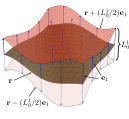
\includegraphics[width=0.8\textwidth]{figs_part2/cosserat_surface/cosserat_kinematics.pdf}
        \caption{The director field $\mathbf{e}_1(u,v)$ (blue arrows) and the midsurface $\mathbf{r}(u,v)$ (brown surface) of the Cosserat surface approximates a thin shell by constraining the material fibres along the director to be fixed. The upper and lower boundaries of the shell (transparent red surfaces) are given by $\mathbf{r}(u,v) \pm (L_0^1 / 2) \mathbf{e}_1(u,v)$ respectively.}
        \label{fig:cosserat surface}
\end{figure}

As we did in Sec.~\ref{sec:Cosserat rod constitutive dynamics} for a slender tube, we will now kinematically approximate the thin shell with a Cosserat system of lower dimensionality. We consider a Cosserat surface, with material base space $M = [0, L_0^2] \times [0, L_0^3]$, and we denote its material coordinates as $(u, v) = (X_2, X_3)$. A single inextensible director $\mathbf{e}_1$ is attached at each material point $(u,v)$. Then, the Cosserat surface approximates the slender body under the kinematic assumption that the fibres along $\mathbf{e}_1$ are rigid bodies. In other words we have
\begin{equation} \label{eq:thin shell kinematic assumption}
\mathbf{x}(\mathbf{X}, t) = \mathbf{r}(t, u, v) + X_1 \mathbf{e}_1.
\end{equation}
where $X_1 \in [-L_0^1/2, L_0^2/2]$ and $\mathbf{r}(t,u,v)$ is the mid-surface. Equation \ref{eq:thin shell kinematic assumption} is illustrated in Fig.~\ref{fig:cosserat surface}. Notably the Cosserat surface only has a single director, as opposed to the two directors of the Cosserat rod. This means that the internal configuration space of the Cosserat surface is $S^2 = SO(3) / SO(2)$ rather than $SO(3)$. However, for the sake of convenience we may add an additional orthonormal director $\mathbf{e}_2$ such that we have a full material frame $E \in SO(3)$. We thus introduce a guage freedom in the physical description of the system, but due to the abelian nature of $SO(2)$ this will not cause any issues in the physical description of the system.

We write $\Phi(t,u,v) = (\mathbf{r}(t, u,v) ; E(t,u,v))$ as before and
\begin{equation}
\xi = N dt + X_u du + X_v dv
\end{equation}
where
\begin{subequations} \label{eq:N X_alpha defs}
\begin{align}
N & = \{ \vec{V}; \vec{\Omega} \} \\
X_u & = \{ \vec{\theta}_u ; \vec{\pi}_u \} \\
X_v & = \{ \vec{\theta}_v ; \vec{\pi}_v \}.
\end{align}
\end{subequations}
From $\Phi^{-1} d \Phi = \xi$ we find
\begin{subequations} 
\begin{align}
d \mathbf{r} & = \mathbf{V} dt + \boldsymbol{\theta}_u du + \boldsymbol{\theta}_v dv  \\
d E & = E \hat{\Omega} dt + E \hat{\pi}_u du + E \hat{\pi}_v dv.
\end{align}
\end{subequations}
and from Eq.~\ref{eq:(summary) geometrised kinematic equations of motion} we find the kinematic equations of motion
\begin{subequations}
\begin{align}
\dot{X}_u & = \mathcal{D}_u N \\
\dot{X}_v & = \mathcal{D}_v N
\end{align}
\end{subequations}
where the spatial reconstruction fields $X_u$ and $X_v$ must obey the spatial integrability conditions
\begin{equation}
\partial_v X_u = \mathcal{D}_u X_v.
\end{equation}

We now derive the dynamical equations of motion. Carrying out the analogous derivation as we did in Sec.~\ref{sec:Cosserat rod constitutive dynamics}, we find that the kinetic energy density per unit material area is
\begin{equation}
\mathcal{K} = \frac{1}{2} \rho_0 |\vec{V}|^2 + \frac{1}{2} \vec{\Omega}^T \mathbb{I} \vec{\Omega} 
\end{equation}
where $\rho_0 = L_0^1 \rho_0^V$ and $\mathbb{I}$ is the moment-of-inertia of the material frame per unit material area.

From Eq.~\ref{eq:(summary) dynamical equations of motion} we find the dynamical equations of motion
\begin{subequations}  \label{eq:surface dynamical eoms}
\begin{align}
\mathcal{D}_t^* S & = \mathcal{D}_u^* Q^u + \mathcal{D}_v^* Q^v + T \\
n_\alpha Q^\alpha & = 0, \quad \text{on } \partial M.
\end{align}
\end{subequations}
where we sum over $\alpha = u,v$ and $\text{ad}_{\cdot}^*$ was given in Eq.~\ref{eq:SE(3) dual adjoint}, and where
\begin{subequations} \label{eq:S Qu Qv}
\begin{align}
S & = \frac{\partial \mathcal{K}}{\partial N} = \{ \vec{P} ; \vec{L} \} \\
Q^u & = \{ \vec{F}^u ; \vec{M}^u \} \\
Q^v & = \{ \vec{F}^v ; \vec{M}^v \}
\end{align}
\end{subequations}
and $\vec{P} = \rho_0 \vec{V}$ and $\vec{L} = \mathbb{I} \vec{\Omega}$.  Substituting Eq.~\ref{eq:N X_alpha defs} and Eq.~\ref{eq:S Qu Qv} into Eq.~\ref{eq:surface dynamical eoms} we get
\begin{subequations} \label{eq:cosserat surface dynamic eoms}
\begin{align}
D_t \vec{P} & = D_\alpha \vec{F}^\alpha + \vec{f} \label{eq:surface P eom} \\
D_t \vec{L} & = D_\alpha \vec{M}^\alpha + \vec{\theta}_\alpha \times \vec{F}^\alpha + \vec{m} \label{eq:surface L eom} \\
n_\alpha \vec{F}^\alpha & = n_\alpha \vec{M}^\alpha = 0, \quad \text{on } \partial M 
\end{align}
\end{subequations}
where we sum over repeated indices of $\alpha = u, v$, and is consistent with the dynamical equations of motion found in the literature \citep{altenbachCosseratMedia2013}. Repeating the same dimensional arguments as in Sec.~\ref{sec:cosserat 3d bodies}, we can conclude that $\vec{P}$ and $\vec{L}$ have units of momentum and angular momentum per unit material area respectively, and $\vec{F}^\alpha$ and $\vec{M}^\alpha$ force and moment per unit material length respectively. The body force $\vec{f}$ and $\vec{m}$ have units of force and moment per unit material area respectively.

Note that the component $L_1$ of the angular momentum of the material frame is unphysical if the Cosserat surface is seen as an approximate model for a slender shell. For conservative dynamics, this means that $\mathcal{U}$ should not couple to $\pi_1$, which is the rate-of-twist of the material frame around $\mathbf{e}_1$. In general, this entails that $M^\alpha_1 = m^\alpha_1 = 0$.

In the above we have considered a rectangular material base space $M$. However, in general for \textit{open} Cosserat surfaces the material base space can be any bounded and compact subset $M \subset \mathbb{R}^2$. Furthermore, \textit{closed} Cosserat surfaces may have $M = S^2$, in which case the material base space no longer admits global coordinates. The kinematic and dynamical equations of motion above still apply in the case of a closed surface, but they must then be simultaneously and consistently simulated over multiple charts that cover $M$.



%\subsubsection{Kinematic constraints}

%We now eliminate the internal degrees of freedom, such that the system configuration is only specified by $\mathbf{r}(t,u,v) \in \mathbb{E}^3$. We will proceed in a manner analogous to Sec.~\ref{sec:Kinematic constraints and gauge freedoms}.

%Similar to the 

%\citep{olverSurveyMovingFrames2005, felsMovingCoframesPractical1998, felsMovingCoframesII1999, altenbachCosseratMedia2013}




\subsection{Cosserat rods on 2-spheres} \label{sec:Cosserat rods on 2-spheres}

We consider the constitutive dynamics of a generalised Cosserat rod, lying on the $2$-dimensional surface of a sphere $S^2 = \{ \mathbf{x} \in \mathbb{E}^3 \ |\ |\mathbf{x}| = r \}$ where $r$ is the radius of the sphere. Some recent applications of such systems can be found in \citep{mannaEmergentTopologicalPhenomena2019, hsuActivityinducedPolarPatterns2022}. The external configuration space of the rod is thus $S^2 = SO(3) / SO(2)$, and the internal configuration space is $SO(2)$. Let $\mathbf{r}(t,u) = r \mathbf{e}_0(t,u)$ denote the center-line of the rod, where $\mathbf{n}(t,u) \in \mathbb{E}^3$ is a unit-vector, and $u \in [0, L_0],\ t \in [0, T]$. The material frame $E = (\mathbf{e}_1(t,u), \mathbf{e}_2(t,u))$ of the rod are two orthonormal vectors that are tangent to $S^2$ at $\mathbf{r}$, and can be seen as an element of $SO(2)$. We also have that the triad $(\mathbf{n}\ \mathbf{e}_1\ \mathbf{e}_2)$ are mutually orthogonal, and $\mathbf{n}(t,u)$ is normal to $S^1$ at $\mathbf{r}(t,u)$ and $(\mathbf{e}_1\ \mathbf{e}_2)$ forms a basis for $T_{\mathbf{r}(t,u)} S^2$. Furthermore, as the triad forms an orthogonal matrix with unit determinant we can identify it as an element of $SO(3)$, and will thus write $\Phi = (\mathbf{n}\ \mathbf{e}_1\ \mathbf{e}_2)$. The configuration space of the Cosserat rod on the sphere is thus $G = SO(3)$, with kinematic base space $W = [0, T] \times [0, L_0]$ which admits a global basis. As in Ch.~\ref{ch:Cosserat rods} we will distinguish between vectors $\mathbf{v} \in \mathbb{E}^3$ in the fixed frame and vectors $\vec{v} \in \mathbb{R}^3$ in the moving frame, and relate the two as $\vec{v} = \Phi^T \mathbf{v}$. We shall write the components of vectors in the moving frame as $\vec{v} = (v_n, v_1, v_2)$.

We shall write the Maurer-Cartan form as
\begin{equation}
\xi = \hat{N} dt + \hat{X} du
\end{equation}
where $\hat{N}(t,u), \hat{X}(t,u) \in \mathfrak{so}(3)$, and we write
\begin{subequations}
\begin{align}
\vec{N} & = (\Omega_n, -V_2/r, V_1/r)^T \\
\vec{X} & = (\pi_n, -\theta_2/r, \theta_1/r)^T 
\end{align}
\end{subequations}
and
\begin{subequations}
\begin{align}
\vec{V} & = (0, V_1, V_2)^T \\
\vec{\theta} & = (0, \theta_1, \theta_2)^T \\
\vec{\Omega} & = (\Omega_n, 0, 0)^T \\
\vec{\pi} & = (\pi_n, 0, 0)^T.
\end{align}
\end{subequations}
From $\Phi^{-1} d \Phi = \xi$ we find
\begin{subequations}
\begin{align}
d \mathbf{r} & = r d \mathbf{n} = \mathbf{e}_i V_i dt + \mathbf{e}_i \theta_i du \\ 
 & = \mathbf{V} dt + \boldsymbol{\theta} du \nonumber \\
d \mathbf{e}_1 & = (\Omega_n \mathbf{e}_2 - (V_1/r) \mathbf{n}) dt + (\pi_n \mathbf{e}_2 - (\theta_1/r) \mathbf{n}) du \\
d \mathbf{e}_2 & = (-\Omega_n \mathbf{e}_1 - (V_2/r) \mathbf{n}) dt + (-\pi_n \mathbf{e}_1 - (\theta_2/r) \mathbf{n}) du.
\end{align}
\end{subequations}
We can identify $\mathbf{V}(t,u) \in T_{\mathbf{r}(t,u)} S^2$ as the velocity of the center-line at $\mathbf{r}(t,u)$ and likewise $\boldsymbol{\theta}(t,u) \in T_{\mathbf{r}(t,u)} S^2$ as the rate-of-change of the center-line along the material coordinate $u$. We can also identify $\Omega_n(t,u)$ and $\pi_n(t,u)$ as the angular velocity and angular rate-of-rotation of the material frame around $\mathbf{n}$, and thus $\Omega(t,u),  \pi(t,u) \in \mathfrak{so}(2)$.

\begin{figure*} 
    \centering
     
    \begin{subfigure}[b]{0.6\textwidth}  
        \centering 
        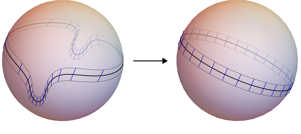
\includegraphics[width=\textwidth]{figs_part2/cosserat_rod_on_spheres/rod_on_sphere.pdf}
        \caption[Overdamped Cosserat rod relaxing to a ground-state]%
        {{\small Overdamped Cosserat rod relaxing to a ground-state}}    
        \label{fig:rod on sphere simulation}
    \end{subfigure}
    \hfill
    \begin{subfigure}[b]{0.32\textwidth}
        \centering
        \includegraphics[width=\textwidth]{figs_part2/cosserat_rod_on_spheres/rod_on_sphere_U.pdf}
        \caption[Potential energy]%
        {{\small Potential energy}}    
        \label{fig:rod on sphere U}
    \end{subfigure}    
    
    \caption[  ]
    {\small (a) Overdamped Cosserat rod on $2$-sphere relaxing from a deformed initial configuration (left) to a ground-state (right). Solid black lines are the rod center-lines, and the blue lines are the directors $\mathbf{e}_2$. (b) Potential energy of the Cosserat rod.} 
    \label{fig:rod on sphere}
\end{figure*}

From Eq.~\ref{eq:(summary) geometrised kinematic equations of motion} we can find the kinematic equations of motion
\begin{equation} \label{eq:cosserat rod on sphere kinematic eoms}
\begin{aligned}
\dot{\vec{X}} & = \mathcal{D}_u \vec{N} \\
& = \vec{N}' + \vec{X} \times \vec{N}
\end{aligned}
\end{equation}
using $\overrightarrow{[\hat{X}, \hat{N}]} = \vec{X} \times \vec{N}$. We define the Lagrangian
\begin{subequations} \label{eq:cosserat rod on sphere lagrangian}
\begin{align}
\mathcal{L}(d \Phi) & = \mathcal{K}(\dot{\Phi})) - \mathcal{U}(\Phi') \\
\mathcal{K} & = \frac{1}{2} \rho_0 |\mathbf{V}|^2 + \frac{1}{2} \mathbb{I}_n \Omega_n^2
\end{align}
\end{subequations}
where $\mathcal{U}$ is constitutive potential energy, $\rho_0$ is the mass density per unit material length and $\mathbb{I}_n \in \mathbb{R}$ is the moment-of-inertia per unit material length of the material frame.  In its reduced form, the Lagrangian is
\begin{subequations} \label{eq:cosserat rod on sphere reduced lagrangian}
\begin{align}
\mathcal{\ell}(\xi) & = \mathcal{K}(N) - \mathcal{U}(X) \\
\mathcal{K} & = \frac{1}{2} \rho_0 |\vec{V}|^2 + \frac{1}{2} \mathbb{I}_n \Omega_n^2.
\end{align}
\end{subequations}
The conjugate moment and stress are $\vec{P} = \frac{\partial \ell}{\partial \vec{N}}$ and $\vec{Q} = -\frac{\partial \ell}{\partial \vec{X}}$ respectively, and we get
\begin{subequations} 
\begin{align}
\vec{P} & = (L_n, p_2 r, - p_1 r)^T \\
\vec{Q} & = (M_n, F_2 r, - F_1 r)^T
\end{align}
\end{subequations}
where $\vec{F} = (0, F_1, F_2)^T$ and $\vec{p} = (0, \rho_0 V_1, \rho_0 V_2)^T$ is the force on the center-line and its linear momentum density per unit material length respectively, and where $\vec{M} = (M_n, 0, 0)$ and $\vec{L} = (\mathbb{I}_n \Omega_n, 0, 0)^T$ are the moment on the material frame and its angular momentum per unit material length respectively. From Eq.~\ref{eq:(summary) dynamical equations of motion} we find the dynamical equations of motion
\begin{subequations} \label{eq:rod on 2-sphere dynamical eoms}
\begin{align}
(\partial_t + \hat{N}) \vec{S} & = (\partial_u + \hat{X}) \vec{Q} + \vec{T} \\
Q_\alpha & = 0, \quad u = 0, L_0.
\end{align}
\end{subequations}
where we used $[\text{ad}_X] = \hat{X}$ and $[\text{ad}^*_X] = -[\text{ad}_X]^T$, and where $\vec{T}$ is a generalised body force. In the absence of body forces, and using the definitions of $S, Q, N$ and $X$, we get
\begin{subequations} 
\begin{align} \label{eq:rod on 2-sphere dynamical eoms 2}
\dot{\bar{L}} & = M' + \vec{\theta} \times \vec{F} \\
\dot{\bar{P}} & = D_u \vec{F} - c \vec{\Omega} \times \vec{V} + \frac{1}{r^2} \vec{M} \times \vec{\theta}
\end{align}
\end{subequations}
where $c = \rho_0 + \mathbb{I}_n/r^2$. $\vec{\theta} \times \vec{F}$ is the moment exerted on the material frame due to the force, $\frac{1}{r^2} \vec{M} \times \vec{\theta}$ is the force exerted on the center-line due to the moment, and $- c \vec{\Omega} \times \vec{V}$ can be seen as a Coriolis force that arises due to the rotating frame. Equations \ref{eq:cosserat rod on sphere kinematic eoms} and \ref{eq:rod on 2-sphere dynamical eoms 2} together form a set of equations that completely determine the kinematics and dynamics of the system.

We will now consider the example of `overdamped' Cosserat rod dynamics on the $2$-sphere. We define the frictional body force $\vec{T} = \gamma \vec{N}$, where $\gamma \in \mathbb{R}^{3\times 3}$ is a symmetric and positive-definite matrix, and the constitutive potential
\begin{equation} \label{eq:cosserat rod on sphere U}
\mathcal{U} = \frac{1}{2} \epsilon (\vec{X} - \vec{X}_0)^T \mathsf{K} (\vec{X} - \vec{X}_0)
\end{equation}
where $\vec{X}_0 = (0\ 1\ 0)^T$ and $\mathsf{K} \in \mathbb{R}^{3 \times 3}$ is a positive definite matrix. We take the overdamped limit, eliminating the inertial degrees of freedom $\vec{P} \approx 0$, to get
\begin{subequations} \label{eq:rod on 2-sphere dynamical eoms overdamped}
\begin{align}
\dot{\vec{X}} & = \vec{N}' + \vec{X} \times \vec{N} \\
\gamma \vec{N} & = (\partial_u + \hat{X}) \vec{Q}.
\end{align}
\end{subequations}
Fig.~\ref{fig:rod on sphere} shows the result of a simulation of Eq.~\ref{eq:rod on 2-sphere dynamical eoms overdamped}, depicting the relaxation of an initial deformed state to a ground-state that minimises Eq.~\ref{eq:cosserat rod on sphere U}.

\subsection{Relativistic Cosserat rods} \label{sec:Relativistic Cosserat rods}

Here we derive the kinematic equations of relativistic motion of a Cosserat rod. We work in units where the speed-of-light constant is set to unity $c= 1$. The Minkowski vector space $\mathbb{M}^{1,3}$ is the vector space $\mathbb{R}^4$ equipped with the \textit{Minkowski inner product} $\langle \cdot, \cdot \rangle_M : \mathbb{M}^{1,3} \times \mathbb{M}^{1,3} \to \mathbb{R}$ with signature $(1, 3)$. In other words, given some basis $B = (\mathbf{b}_0, \mathbf{b}_1, \mathbf{b}_2, \mathbf{b}_3)$ for $\mathbb{R}^4$, the \textit{Minkowski metric}
\begin{equation}
\eta_{ij} = \langle \mathbf{b}_i, \mathbf{b}_j \rangle_M
\end{equation}
has $1$ negative eigenvalue and $3$ positive eigenvalues. Henceforth we will assume that the basis is defined such that
\begin{equation} \label{eq:eta diagonalised}
\eta = \text{diag}(-1, 1, 1, 1).
\end{equation}
Any basis that diagonalises $\eta$ as in Eq.~\ref{eq:eta diagonalised} will be called an \textit{orthonormal} basis. A $\mathbf{v} \in \mathbb{M}^{1,3}$ is known as \textit{time-like} if $\langle \mathbf{v}, \mathbf{v} \rangle_M < 0$, \textit{space-like} if $\langle \mathbf{v}, \mathbf{v} \rangle_M > 0$ and \textit{light-like} if $\langle \mathbf{v}, \mathbf{v} \rangle_M = 0$. We can thus identify $\mathbf{b}_0$ as the time-like direction in this basis, and $(\mathbf{b}_1, \mathbf{b}_2, \mathbf{b}_3)$ as the space-like directions.

The \textit{space-time coordinates} $\mathbf{r}(\tau)$ of an observer is a function $\mathbf{r} : \mathbb{R} \to \mathbb{M}^{1,3}$ where $\tau$ is the time measured by clocks co-moving with the observer, known as the \textit{proper time}. The \textit{$4$-velocity} of the observer is given by the time-like vector $\mathbf{U} = \partial_\tau \mathbf{r}$. The \textit{inertial frame} of the observer at proper time $\tau$ is an orthonormal basis $E(\tau) = (\mathbf{e}_0(\tau), \mathbf{e}_1(\tau), \mathbf{e}_2(\tau), \mathbf{e}_3(\tau))$ such that
\begin{equation}
\vec{U} = E^{-1} \mathbf{U} = (1\ 0\ 0\ 0)^T.
\end{equation}
Intuitively, this corresponds to the fact that an observer is always stationary in its own co-moving inertial reference frame. Such a basis can be found by setting $\mathbf{e}_0 = \mathbf{U}$, and the remaining three basis elements $(\mathbf{e}_1, \mathbf{e}_2, \mathbf{e}_3)$ specify the spatial orientation of the observer. Vectors $\vec{v} = E^{-1} \mathbf{v}$ are thus expressed in the inertial frame $E$. We shall use the notation $\tilde{v}$ to refer to the spatial components of $\vec{v}$, such that $\vec{v} = (v_0\ \tilde{v}^T)^T$.


Any two inertial frames $E_1$ and $E_2$ can be related by a \textit{Lorentz transformation}
\begin{equation} \label{eq:E1 E2 lorentz relation}
E_2 = \Lambda E_1
\end{equation}
where $\Lambda \in SO(1, 3)$, and where $SO(1, 3)$ is the \textit{Lorentz group} on $\mathbb{M}^{1,3}$ and is defined as
\begin{equation}
SO(1, 3) = \{ \Lambda \in \mathbb{R}^{4 \times 4} \ |\ \langle \Lambda \mathbf{v}, \Lambda \mathbf{v} \rangle_M = \langle \mathbf{v}, \mathbf{v} \rangle_M\ \forall \mathbf{v} \in \mathbb{M}^{3,1 } \}.
\end{equation}
which is the group of rotations in space and \textit{Lorentz boosts}. The Lorentz group is thus the set of linear transformations that preserves the Minkowski inner product. Combined with the group of translations on $\mathbb{M}^{1,3}$, we have the \textit{Poincaré} group
\begin{equation}
M(1,3) = \left\{
\begin{pmatrix}
1 & \mathbf{0}^T \\
\mathbf{t} & \Lambda
\end{pmatrix} \in \mathbb{R}^{5 \times 5}\ |\ \mathbf{t} \in \mathbb{M}^{1,3},\ \Lambda \in SO(3,1) 
\right\}
\end{equation}
of space-time translations and rotations.

Now consider a continuous `string' of inertial observers with space-time coordinates $\mathbf{r}(\tau, u)$ and inertial frames $E(\tau, u)$, parametrised by $u$. If $\mathbf{e}_0(\tau, u) = \partial_\tau \mathbf{U}(\tau, u)$ then this can be considered a \textit{relativistic} Cosserat rod, where $(\mathbf{e}_1, \mathbf{e}_2, \mathbf{e}_3)$ is here the material frame of the rod. In order to avoid confusing using the word `frame` in reference to both material and inertial frames, we will henceforth refer to the former as the Cosserat cross-section. Given a reference frame $B$ and origin $\mathbf{0} \in \mathbb{M}^{1,3}$, we can write the configuration of the Cosserat rod as
\begin{equation}
\mathcal{F} = \mathcal{F}_0 \Phi
\end{equation}
where
\begin{equation}
\mathcal{F} = (\mathbf{r} ; E ) = \begin{pmatrix}
1 & \mathbf{0}^T \\
\mathbf{r} & E
\end{pmatrix}
\end{equation}
and $\mathcal{F}_0 = (\mathbf{0} ; B)$ and $\Phi = (B^{-1} \mathbf{r} ; B^{-1} \Lambda B)$, and where $\Lambda$ satisfies $E = \Lambda B$. As in Sec.~\ref{sec:Lie group–Lie algebra correspondence}, we now simplify our notation by letting $B = \mathbbm{1}_{4 \times 4}$, such that $\Lambda = E \in SO(1,3)$ and we can thus write $\Phi = \mathcal{F}$. 

We write the Maurer-Cartan form as
\begin{equation}
\xi = N d \tau + X du
\end{equation}
where
\begin{subequations}
\begin{align}
N & = \{ \vec{U} ; O \} = \begin{pmatrix}
0 & \vec{0}^T \\
\vec{U} & O
\end{pmatrix} \\
X & = \{ \vec{\theta} ; \Xi \} = \begin{pmatrix}
0 & \vec{0}^T \\
\vec{\theta} & \Xi
\end{pmatrix} 
\end{align}
\end{subequations}
and $N(\tau, u), X(\tau, u) \in \mathfrak{m}(1,3)$ and $O, \Xi \in \mathfrak{so}(1,3)$. From $\Phi^{-1} d \Phi = \xi$ we find
\begin{subequations}
\begin{align}
d \mathbf{r} & = \mathbf{U} d \tau + \boldsymbol{\theta} du \\
 & = \mathbf{e}_0 d \tau + \boldsymbol{\theta} du \nonumber \\
d \mathbf{e}_\beta & = \mathbf{e}_\alpha O_{\alpha \beta} d\tau + \mathbf{e}_\alpha \Xi_{\alpha \beta} du,\ \alpha,\beta = 0,1,2,3
\end{align}
\end{subequations}
where we used $\mathbf{e}_0 = \mathbf{U}$, which should be seen as a kinematic restriction on the Lie group-valued $\Phi$ (although note that it is not a kinematic restriction from the physical perspective, as real inertial observers always are always stationary with respect to themselves). Because we have parametrised the Cosserat rod with respect to the co-moving inertial frames, we have that $\vec{U}(\tau, u) = (1\ 0\ 0\ 0)^T$. Therefore the kinematic movement of the rod is not specified in $\vec{U}$ as in Sec.~\ref{sec:Geometric Cosserat rod mechanics}, but must instead be encoded in $O$.

The Lie algebra element $O \in \mathfrak{so}(1,3)$ can be written as
\begin{equation}
O = \begin{pmatrix}
0 & \tilde{a}^T \\
\tilde{a} & \hat{\tilde{\Omega}}
\end{pmatrix}
\end{equation}
where $\tilde{a} = (a_1, a_2, a_3)$ and $\hat{\tilde{\Omega}} \in \mathfrak{so}(3)$. Henceforth the tilde will designate spatial $3$-vectors. To interpret these quantities, we first note that
\begin{equation}
\partial_\tau \mathbf{e}_i = \mathbf{e}_i \hat{\tilde{\Omega}}_{ij},\ i=1,2,3
\end{equation}
from which we identify that $\tilde{\Omega}(\tau, u)$ is the angular velocity of the Cosserat cross-section at $u$ in its inertial frame. Secondly, we can compute the \textit{$4$-acceleration} $\mathbf{a} = \partial_\tau^2 \mathbf{r}$ as
\begin{equation} \label{eq:4-acceleration}
\mathbf{a} = \partial_\tau \mathbf{e}_i = \mathbf{e}_i a_i,\ i=1,2,3.
\end{equation}
such that $\vec{a} = E^{-1} \mathbf{a} = (0\ \tilde{a}^T)^T$, which is the correct expression for the co-moving 4-acceleration in special relativistic kinematics \citep[p.~99]{rindlerRelativitySpecialGeneral2001}. We thus see that $\tilde{a}(\tau, u)$ is the acceleration of the Cosserat cross-section at $u$ in its co-moving inertial frame. Therefore the kinematics of the relativistic Cosserat rod is specified by the spatial acceleration $\tilde{a}$ of the center-line and the angular velocity $\tilde{\Omega}$ of the cross-section. This stands in contrast to the non-relativistic Cosserat rod, where we instead specify the velocity of the center-line. We can understand this difference by noting that velocity is \emph{itself} a kinematic degree of freedom in special relativity, in addition to position and orientation. Only the latter two are kinematic degrees of freedom in non-relativistic systems. Mathematically, we have that the relative velocity of an inertial observer with frame $E_1$ with respect to another observer with frame $E_2$ is encoded in the Lorentz transformation that relates the two, as in Eq.~\ref{eq:E1 E2 lorentz relation}. This is therefore the reason why we must specify the \emph{acceleration} of the frame, as opposed to its \emph{velocity}, in the kinematics.

The kinematic equations of motion are given by Eq.~\ref{eq:(summary) geometrised kinematic equations of motion}, from which we find
\begin{subequations}
\begin{align}
\partial_\tau \vec{\theta} & = - O \vec{\theta} + \Xi \vec{U} \\
\partial_\tau \Xi & = \partial_u O + [\Xi, O].
\end{align} 
\end{subequations}
If we let
\begin{equation}
O = \begin{pmatrix}
0 & \tilde{t}^T \\
\tilde{t} & \hat{\tilde{\pi}}
\end{pmatrix}
\end{equation}
then the kinematic equations of motion can be written as
\begin{subequations}
\begin{align}
\partial_\tau \theta_0 & = a_i \theta_i \\
\tilde{D}_\tau \tilde{\theta} & = - \theta_0 \tilde{a} + \tilde{t} \\
\tilde{D}_\tau \tilde{t} & = \tilde{D}_u \tilde{a} \\
\partial_\tau \tilde{\pi} & = \tilde{D}_u \tilde{\Omega}
\end{align} 
\end{subequations}
where $i = 1,2,3$ and $\tilde{D}_\tau = \partial_\tau + \hat{\tilde{\Omega}}$ and $\tilde{D}_u = \partial_u + \hat{\tilde{\pi}}$.

% https://en.wikipedia.org/wiki/Relativistic_mechanics

% https://en.wikipedia.org/wiki/Four-velocity

% https://en.wikipedia.org/wiki/Poincar%C3%A9_group

% https://farside.ph.utexas.edu/teaching/em/lectures/node115.html

% https://physics.stackexchange.com/questions/318361/is-my-interpretation-of-dt-d-tau-correct

% https://en.wikipedia.org/wiki/Relativistic_Lagrangian_mechanics

% https://en.wikipedia.org/wiki/Relativistic_angular_momentum

% https://physics.stackexchange.com/questions/520222/when-we-calculate-the-relativistic-angular-momentum-of-a-particle-in-the-directi

%\subsection{Nematic materials}

%$RP^2 \cong S^2/~$

%https://math.stackexchange.com/questions/1391724/real-projective-plane-is-same-as-identifying-antipodal-boundary-points-of-the-2

% https://math.stackexchange.com/questions/2876529/how-can-a-representation-of-so3-be-more-than-3-dimensional

% https://math.stackexchange.com/questions/4268711/why-does-a-space-of-symmetric-traceless-tensors-form-an-irreducible-representati

% https://math.stackexchange.com/questions/3626821/spherical-harmonics-and-irreducible-representations-of-so2-and-so3

% http://visuallietheory.blogspot.com/2013/07/real-representations-of-lie-algebra.html

\subsection{The $O(N)$ non-linear $\sigma$ model} \label{sec:The O(3) non-linear sigma model}

Here we give an example of the geometrisation programme applied to a field theory. We consider a field $\vec{n} : W \to S^N \subset \mathbb{R}^N$, where $W$ is the base space and $\vec{n}$ is a unit-vector in $\mathbb{R}^N$ for all $p \in W$. We call $S^N \subset \mathbb{R}^N$ the \textit{target manifold} of the field theory. We let $W = \mathbb{M}^{1,d}$, which is the $(d+1)$-dimensional Minkowski space, although what follows is easily generalisable to Euclidean space or any arbitrary base space.  
 We define coordinates $(t, u^1, u^2, \dots, u^d)$ on $\mathbb{M}^{1,d}$, and we will write partial derivatives as $\partial_\gamma,\ \gamma=0,1,\dots,d$, where $\partial_0 = \frac{\partial}{\partial t}$ and $\partial_\alpha = \frac{\partial}{\partial u^\alpha},\ \alpha=1,\dots,d$.

The \textit{$O(N)$ non-linear $\sigma$ model} \citep{ketovQuantumNonlinearSigmaModels2013} is defined by the Lagrangian density
\begin{equation} \label{eq:O(N) model}
\mathcal{L} = \frac{1}{2} \eta^{\gamma \kappa} (\partial_\gamma \vec{n})^T (\partial_\kappa \vec{n}) 
\end{equation}
which is expressed in some local coordinate chart of $\mathbb{M}^{1,d}$, where $\eta$ is the Minkowski metric on $\mathbb{M}^{1,d}$ with signature $(1,d)$.

Let the $SO(N)$-valued field $\Phi : \mathbb{M}^{1,d} \to SO(3)$ satisfy $\vec{n} = \Phi \vec{n}_0$ where $\vec{n}_0 \in S^N$ is some constant reference vector. We can then rewrite Eq.~\ref{eq:O(N) model} as
\begin{equation}
\mathcal{L} = \frac{1}{2} \eta^{\gamma \kappa} (\partial_\gamma \Phi \vec{n}_0)^T (\partial_\kappa \Phi  \vec{n}_0) 
\end{equation}
Now, we have
\begin{equation}
\begin{aligned}
(\partial_\gamma \Phi \vec{n}_0)^T (\partial_\kappa \Phi  \vec{n}_0) & = (\Phi^{-1} \partial_\gamma \Phi \vec{n}_0)^T (\Phi^{-1} \partial_\kappa \Phi  \vec{n}_0) \\
& = (\hat{Z}_\gamma \vec{n}_0)^T (\hat{Z}_\kappa \vec{n}_0)
\end{aligned}
\end{equation}
for all $\gamma,\kappa = 1,\dots, d$, where we have defined $\hat{Z}_\gamma = \Phi^{-1} \partial_\gamma \Phi \in \mathfrak{so}(N)$. As before we will  be making use of the hat-map to convert anti-symmetric $3\times 3$-matrices $\hat{Z}_\gamma$ to $3$-vectors $\vec{Z}_\gamma$. Let us now assume that the coordinates are defined such that $\eta = \text{diag}(-1, 1, \dots, 1)$. The Lagrangian then has a reduced form
\begin{equation}
\ell(\xi) = - \frac{1}{2} \vec{N}^T \mathsf{N}_0 \vec{N} + \frac{1}{2} \sum_{\alpha=1}^d \vec{X}_\alpha^T \mathsf{N}_0 \vec{X}_\alpha
\end{equation}
where $\vec{N} = \vec{Z}_0$ and $\vec{X}_\alpha = \vec{Z}_\alpha,\ \alpha = 1, \dots, d$ and $\mathsf{N}_0 = \hat{n}_0^T \hat{n}_0$ and we have used $|\hat{Z}_\gamma \vec{n}_0 | = |\vec{Z}_\gamma \times  \vec{n}_0 | = | \hat{n}_0 \vec{Z}_\gamma  |$.

We can then readily apply the geometrisation programme to the system, to get the field equations of motion
\begin{subequations} 
\begin{align}
\partial_t \vec{X}_\alpha & = (\partial_\alpha + \hat{X}_\alpha) N \\
(\partial_t + \hat{N}) \vec{S} & = \sum_{\alpha=1}^d (\partial_\alpha + \hat{X}_\alpha) \vec{Q}^\alpha  \label{eq:dynamic field equations}
\end{align}
\end{subequations}
where $\vec{N} = \vec{Z}_0$, $\vec{X}_\alpha = \vec{Z}_\alpha,\ \alpha = 1, \dots, d$, $S = \frac{\partial \ell}{\partial N}$ and $Q^\alpha = \frac{\partial \ell}{\partial X_\alpha}$. The spatial reconstruction fields $X_\alpha$ must satisfy the spatial integrability conditions
\begin{equation}
\partial_\beta X_\alpha = \mathcal{D}_\alpha X_\beta
\end{equation}
at all times $t$, where $\alpha = 1, \dots, d-1$ and $\beta = \alpha+1, \dots, d$.

Note that only two of the three components of $S$ are independently determined by Eq.~\ref{eq:dynamic field equations}, as $\mathsf{N}_0$ is only a rank 2 matrix. To see this let $\vec{n}_0 = (1\ 0\ 0)^T$ such that $\mathsf{N}_0 = \text{diag}(0,1,1)$. We then have that $\vec{S} = (0, N_2, N_3)$ and $Q^\alpha = (0, X_2, X_3)$. This reflects the fact that rotations of $\vec{n}$ around its own axis is a gauge freedom in our formulation of the $O(N)$ non-linear $\sigma$ model.


\begin{comment}

----

On the section for dynamics of homogeneous spaces, recreate the derivation in \citep{poincareFormeNouvelleEquations1901} but where you use your generalised Lagrange-D'Alembert principle.

----

You'll be writing down the Lagrange-Dalembert for the general case of submanifolds of Lie groups. You'll have to motivate what it even means to have an action principle for an abstract system like this where you have not specified exactly what the system even represents. The point is that \textit{if} you have specified some d'Alembert Lagrange dynamics on the level of the Lie group, then it is the case that the reduced d'Alemebert Lagrange dynamics are \textit{equivalent}.

Therefore, programmatically, we can say that to specify the dynamics we first formulate it on the Lie group (which is essentially the program in \citep{alvesMethodVirtualPower1993}), which is often more straightforward and intuitive, and then we reduce it to a Lie algebraic description.

So we start with something like this (have to find the correct version)

\begin{equation}
\int_W ( P_i \delta \dot{q}_i - Q_i \delta q_i) dt \wedge du + \int \mathbf{T}(\delta \Phi) dt \wedge du 
\end{equation}

Programatically, the steps are:

\begin{itemize}
\item Specify the system in some coordinatised way. In the case of a slender tube, we identified that the system can be kinematically approximated as a center-line with a material frame attached, which is the Cosserat rod.

\item Write down the kinetic energy, and the constitutive and body forces and moments acting on it, and write down the Lagrange-D'Alembert principle.

\item If it is the case, identify an isomorphism between the system configuration space and a Lie group. 

\item Using the MC form, derive the kinematic equations of motion.

\item In the Lie group-level dynamics, write the kinetic energy in terms of the Lie algebra. Likewise constrain the constitutive force to be a function of the Lie algebra. If you have a constitutive potential, you need to write it in terms of the Lie algebra. Body forces can in general be functions of both Lie group and Lie algebra. Thus write down the reduced Lagrange-D'Alembert principle.

\item From the reduced Lagrange-D'Alembert principle, derive the dynamical equations of motion.

\item If the configuration space is a homogeneous space, the same steps above apply. The final step is to choose an adapted frame, a gauge choice, with which the constrain the kinematics.

\end{itemize}

Perhaps these steps should have their own section, where I go through each step as a subsection and I provide examples.

\end{comment}








\chapter{Geometric numerical integrators}

\section{Geometric numerical integrators for sub-manifolds of Lie groups}

\section{Geometric numerical integrators for Cosserat rods}

\section{Geometric numerical integrators for Cosserat surfaces}

\section{Geometric numerical integrators for Cosserat rods on 2-spheres}




\chapter{Conclusion}




\bookmarksetup{startatroot}
\chapter*{Summary}
\addcontentsline{toc}{chapter}{Summary}
 
The research presented in this thesis divides into two parts. In the first part, we studied and developed methods for studying the transition path ensemble of It\^{o} diffusion equations. In the second part, we developed a geometric theory of continuum mechanics of systems with Lie group- or homogeneous configuration spaces. Below we summarise the main results of each chapter of the two research streams discussed in this thesis.


In Ch.~\ref{ch:Ritz methods for Freidlin-Wentzel-Graham actions} we began our exploration of the transition path ensemble by considering the Freidlin-Wentzell limit, which corresponds to a limit of vanishing diffusivity. We presented numerical methods for computing most probable transition paths and quasi-potentials of general It\^{o} diffusion equations with additive noise. The method directly minimises the Freidlin-Wentzell action, which allowed for flexibility in choosing the path parametrisation. It uses numerical quadrature to reduce the action to a multivariate function, whose minimum is obtained by either gradient-free and gradient-based optimisation. This provides both the minimum action path and quasipotential. The direct method consisted of a discretisation of the Freidlin-Wentzell action, followed by a search for the minimum in the resulting finite-dimensional space. This approach is algorithmically simple and we showed its accuracy and efficiency on a number of benchmark problems.

In Ch.~\ref{ch:Monte Carlo methods in Path Spaces} we considered the TPE at finite temperatures. We applied recent mathematical developments in the field of functional Markov chain Monte Carlo methods to the sampling of stochastic transition pathways. On this foundation, we developed an MCMC scheme designed to sample TPEs with multiple competing transition channels, which we called the teleporter MCMC. The method was based on a semi-classical expansion of the path-probability measure around the dominant transition pahs of the distribution, with which we constructed independence samplers allowing for the MCMC to intermittently `teleport' between transition channels. Akin to the Ritz method of the Ch.~\ref{ch:Ritz methods for Freidlin-Wentzel-Graham actions}, the MCMC procedures were discretised using a global spectral basis. Speficially, we expanded stochastic paths in the Kosambi-Karhunen-Lo\`eve of the Brownian bridge process. We showed that spectrum of modes in this expansion can be separated into high- and low-frequency bands, where only the lower-band modes are non-trivially distributed, whilst the statistics of the latter is indistinguishable from that of free diffusion. Future research directions may involve devising multi-level MCMC schemes designed around band-structure of the KKL-based methods we developed in this chapter. Furthermore, we may consider extending the algorithm to sample transition path ensembles of field theories. 

In Ch.~\ref{ch:Diffusivity dependence of transition paths} we studied the concentration of competing transition channels in the transition path ensemble, as a function of diffusivity. Using two model systems, we showed that the dominant transition channel does not in general coincide with most probable paths of the path measure, even in a low-to-intermediate temperature regime. We approximated the TPE as mixed Gaussian measures using the semi-classical expansions developed in the previous chapter, using which we constructed semi-analytical approximators of channel rate probabilities. In the regime of validity of these approximators, we showed that the relative dominance of transition channels is a conspiracy between the path-probability of the instanton, reflecting the energetic cost of transition, and Gaussian normalisation constants, reflecting the fluctuations around the instanton.

In Ch.~\ref{sec:geometry introduction} we began our study of the geometric continuum mechanics of systems with Lie group- or homogeneous configuration spaces. We reviewed the classical theories that our work builds on, and developed the necessary mathematical tools for the results of the subsequent chapters. Of these, the mathematical preliminaries, though dense, by itself foreshadows and serves as a dry-run for the geometrical treatment that was to come.

In Ch.~\ref{ch:Cosserat rods} we derived the kinematic and dynamic - in short, kinodynamic - equations of Cosserat rods and filaments. These were chosen as paradigmatic examples of systems with Lie group- and homogeneous configuration spaces, and served as a foundation for the generalisations of the chapter that followed. We identified the configuration space of the Cosserat rod as the special Euclidean group $SE(3)$, and used the Euler-Poincaré theorem to find conservative force and moment balance equations. Furthermore, we constructed a generalised Lagrange-D'Alembert principle from which arbitrary non-conservative dynamics can be derived, and expressed the resulting kinodynamic equations of motion in terms of a spatial reconstruction field $X$ and generalised momentum field $S$, which are defined on the Lie algebra and its dual respectively. This Lie algebraic formulation was shown to naturally lead to kinodynamics expressed in terms of the intrinsic geometry of the rod. We then studied the filament model, which we devised as a Cosserat rod subject to kinematic constraints, and found its kinodynamic equations of motion. We thus demonstrated how systems with homogeneous configuration spaces can be obtained by imposing kinematic constraints on Lie group-configured systems.

In Ch.~\ref{ch:Geometric continuum mechanics on homogeneous configuration spaces} we studied generalised Cosserat systems, which we defined as continuum bodies with a material base of general topology, and Lie group- or homogeneous configuration spaces. We formulated a general theory of the kinodynamics of such systems, which we called a generalised geometric Cosserat theory (GGCT). The cornerstone of the programme was to use the exponential map to relate the spatio-temporal configuraiton of the system to Lie algebra-valued reconstruction fields. This allowed us to express the kinodynamics of generalised Cosserat systems directly in terms of its intrinsic geometry. We applied the GGCT to derive the kinodynamic equations of motion for a variety of known and new systems, which included the classical suite of Cosserat surfaces and bodies, Cosserat rods on spheres and in Minkowski space, as well as an application for non-linear $\sigma$ field theory.

In Ch.~\ref{ch:Geometric numerical integrators} we developed geometric integrators for generalised Cosserat systems. We saw this as an application of Lie group integration theory to the infinite-dimensional setting of continuum systems. We demonstrated that our integrators preserve spatial integrability using the example of a Cosserat surface, and compared their performance to standard non-geometrical numeric integrators. We also showed that other qualitative features, like the closure of a rod, are preserved by our integrators.






%%%%%%%%%%%%%%%%%%%%%%%%%%%%%%%%%%%%%%%%%%%%%%%%%%%%%%%%%%%%%%%%%%%%%%%%%%%%%%%%
%% References:
%%
% If you include some work not referenced in the main text (e.g. using \nocite{}), consider changing "References" to "Bibliography".
%

% \renewcommand to change default "Bibliography" to "References"
\renewcommand{\bibname}{References}
\cleardoublepage
\phantomsection
\addcontentsline{toc}{chapter}{References}
%\bibliographystyle{plainnat}

\bibliographystyle{unsrtnat}
%\bibliography{refs/parti, refs/partii, refs/fluctuations_around_instantons, refs/nucleation, refs/path-integrals, refs/rare_events, refs/diffus_refs1, refs/diffus_refs2}
\bibliography{refs/parti, refs/partii}





%%%%%%%%%%%%%%%%%%%%%%%%%%%%%%%%%%%%%%%%%%%%%%%%%%%%%%%%%%%%%%%%%%%%%%%%%%%%%%%%
%% Appendix:
%%

\cleardoublepage
\phantomsection
\appendix
\addcontentsline{toc}{part}{Appendices}

%\begin{appendices}

%\chapter{Moving frames for sub-manifolds of $SE(d)$} \label{app:Moving frames for sub-manifolds of SE(d)}

\chapter{MCMC benchmark models} \label{app:MCMC benchmark models}

Here we define the Langevin model systems considered in Ch.~\ref{ch:Monte Carlo methods in Path Spaces} and Ch.~\ref{ch:Diffusivity dependence of transition paths}. We begin by defining a non-dimensionalised formulation of the Langevin equation with additive noise
\begin{equation}
d\mathbf{X}=\mu\mathbf{F}dt+\sqrt{2D}d\mathbf{W}.
\end{equation}
where $\mu$ is the mobility constant and $D$ the diffusion constant. We write the latter as $D = \mu k_B \theta$, where $k_B$ is the Boltzmann constant $\theta$ is the temperature. We assume that the force is the gradient of a potential energy function $U : \mathbb{R}^d \to \mathbb{R}$  as $\mathbf{F} = - \nabla \cdot U$.

Let $T_{0}=\frac{L^{2}}{k_{B}\theta_{0}\mu}$ be a time-scale, $\theta_{0}$ a temperature-scale, and $L_0$ a characteristic length-scale of the potential. We set $t=T_{0}\tilde{t}$,
$\theta=\theta_{0}\tilde{\theta}$, $\mathbf{X}=L_0 \tilde{\mathbf{X}}$,
$\mathbf{F}= \frac{\tilde{U}_0}{L_0} \tilde{\mathbf{F}}$ and $\mathbf{W}=\sqrt{T_{0}}\tilde{\mathbf{W}}$. $T_{0}$ is the typical diffusion time-scale at temperature $\theta_{0}$. We get
\begin{equation}
	d\mathbf{\tilde{X}}=\tilde{U}_{0} \tilde{\mathbf{F}}d\tilde{t}+\sqrt{2\tilde{\theta}}d\tilde{\mathbf{W}}.
\end{equation}
where all quantities in the equation are now non-dimensional, and where $\tilde{U}_{0}=\frac{U_{0}}{k_{B}\theta_{0}}$ is the ratio
of the energetic well-depth $U_{0}$ and the thermal energy at temperature $\theta_{0}$. We set $\tilde{U}_0 = 1$, such that $\theta = \theta_0$ corresponds to the temperature at which $U_0 = k_B \theta_0$. In other words, the characteristic energy scale of the potential is equal to the thermal energy at temperature $\theta_0$. Finally, the non-diemsionalised Langevin equation is
\begin{equation}
	d\mathbf{\tilde{X}}= \tilde{\mathbf{F}}d\tilde{t}+\sqrt{2\tilde{\theta}}d\tilde{\mathbf{W}}.
\end{equation}

\section{The asymmetric double-well system} \label{app:The asymmetric double-well system}

\begin{figure}[t]
\includegraphics[width=0.6\textwidth]{figs_part1/mcmc/1D_process_potential}
\centering \caption{The asymmetric double-well potential, with minima at $x/L_0 = -1$ (hollow red circle) and $x/L_0=1$ (filled red circle). See App.~\ref{app:The asymmetric double-well system} for its definition.}
\label{fig:1D process potential} 
\end{figure}

Consider a $1$-dimensional Langevin system with a quartic potential
\begin{equation} \label{eq:general quartic potential}
	U(x) = U_0 \left( 1 + a \frac{x}{L_0} + b \left( \frac{x}{L_0} \right)^2 + x \left( \frac{x}{L_0} \right)^3  + d \left( \frac{x}{L_0} \right)^4  \right).
\end{equation}
We impose the following conditions
\begin{enumerate}
\item $U'(-L_0) = U'(L_0) = 0$. Extrema at $x = -L_0$ and $x= L_0$.
\item $U(-L_0) = 0$ and $U(L_0) = \Delta U$. The energy cost of moving from the left-most extremum to the right-most extremum is $\Delta U$.
\end{enumerate}
Imposing the conditions on Eq.\ref{eq:general quartic potential}, we get
\begin{equation}  \label{eq:asymmetric double well}
U(x)= \left( \left(\frac{x}{L_0}-1\right)^{2}-\frac{1}{4}\frac{\Delta U}{U_{0}}\left(\frac{x}{L_0}-2\right)\right)\left(\frac{x}{L_0}+1\right)^{2}. 
\end{equation}
Equation \ref{eq:asymmetric double well} defines an \textit{asymmetric} variant of a standard quartic double-well system, with minimii at $\frac{x}{L_0}= -1$ and $\frac{x}{L_0}=1$, and a maximum at $\frac{x}{L_0} = \frac{ 3 \Delta U}{16 U_0}$. See Fig.~\ref{fig:1D process potential} for a depiction of the potential energy landscape. In non-dimensionalised form, the potential is
\begin{equation}  \label{eq:asymmetric double well nondim}
\tilde{U}(\tilde{x})= \left( \tilde{x}-1\right)^{2} - \frac{1}{4} \frac{\Delta U}{U_{0}} \left( \tilde{x}-2 \right) \left(\tilde{x}+1\right)^{2}. 
\end{equation}
where $\tilde{x} = x / L$. In all numerical simulations, we have set $\frac{\Delta U}{U_{0}}=1/2$.

\section{The switch system} \label{app:The switch system}

Here we define the \textit{switch} system, and its non-conservative variant used in Ch.~\ref{ch:Diffusivity dependence of transition paths}. We consider a $2$-dimensional Langevin system with a Sombrero-type potential $U : \mathbb{R}^2 \to \mathbb{R}$. Let $\Gamma=\{(x,y)\ |\ \sqrt{x^2 + y^2} =1\}$ be the circle centred around the origin, and let $\Gamma^{+}$ and
$\Gamma^{-}$ signify the upper and lower semi-circle respectively. We will a construct the potential such that $\Gamma$ coincides with a manifold of potential minima, and such that the perpendicular curvature of the potential along $\Gamma^{+}$ is larger than along $\Gamma^{-}$. We
start with a radial quartic potential of the form 
\begin{align}
U(x_{1},x_{2}) & =U_{r}(r(x_{1},x_{2}))\\
U_{r}(r) & =U_{0}\left(\frac{r}{L_0}-1\right)\left(1+a\frac{r}{L_0}+b\left(\frac{r}{L_0}\right)^{2}+c\left(\frac{r}{L_0}\right)^{3}\right)\nonumber 
\end{align}
where $L_0$ is the length-scale of the system, $U_{0}$ will be the
value of the potential at the local maximum $r=0$, and $a,b,c\in\mathbb{R}$
will be specified below. We will henceforth suppress the argument of
the radial coordinate function $r(x_{1},x_{2})=\sqrt{x_{1}^{2}+x_{2}^{2}}$. We
impose the following conditions on the potential to fix $a, b$ and $c$:
\begin{enumerate}
\item $U_r'(0) = 0$. The origin is an extremum.
\item $U_r'(L_0) = 0$. $\Gamma$ is an extremum of the potential.
\item $U_r''(L_0) = k$. The curvature along $\Gamma$ is $k$.
\end{enumerate}
We get
\begin{equation}
U_{r}(r)=\frac{1}{2}\left(\frac{r}{L_0}-1\right)^{2}\left[L_0^{2} k \left(\frac{r}{L_0}\right)^{2}-2U_{0}\left(\frac{r}{L_0}-1\right)\left(3\frac{r}{L_0}+1\right)\right]
\end{equation}
which is, in the non-dimensionalised form
\begin{equation}
\tilde{U}_{r}(\tilde{r})= \frac{1}{2} 
\left( \tilde{r} -1 \right)^{2} \left[L_0^{2} \tilde{k} \tilde{r}^{2}-2  
\left(\tilde{r}-1\right)\left(3\tilde{r}+1\right)\right].
\end{equation}
where $\tilde{r} = r / L$ and $\tilde{k} = \frac{k}{U_0}$. In order to ensure that the potential has a Sombrero-like form, we
must further have that the potential is confining, which is equivalent
to $\underset{r\to\infty}{\lim}U_{r}(r)=\infty$, which implies that
$6U_{0}\leq L_0^{2}k$. We now introduce an angular dependence in the
curvature. We set
\begin{equation}
L_0^{2}k(\phi)=6U_{0}(1+2h(\phi))\label{eq:curvature}
\end{equation}
where $\phi=\phi(x_{1},x_{2})$ is the angle of $(x_{1},x_{2})$ in
polar coordinates so that $x_{1}=\cos(\phi)$, $x_{2}=\sin(\phi)$,
and where
\begin{equation}
h(\phi)=\frac{1}{4}\left(\xi_{2}+\xi_{1}+(\xi_{2}-\xi_{1})\sin\phi\right)
\end{equation}
where $\xi_{2}>\xi_{1}$, and where $h(\phi)\in[\xi_{1},\xi_{2}]$
satisfies $h(-\pi/2)=\xi_{1}$ and $h(\pi/2)=\xi_{2}$. Eq.~\eqref{eq:curvature}
is constructed so that the perpendicular curvature of $\Gamma^{+}$
is larger than that of $\Gamma^{-}$. The drift of the system is now
given by $\mathbf{F}=-\nabla U$. This concludes the definition of the switch system.

We also consider a non-conservative variant of the switch system. We introduce an additional non-conservative
force $\mathbf{F}^{a}=-\eta\hat{\boldsymbol{\phi}}$ for which the
work done in a displacement $d\mathbf{x}=dr\hat{\mathbf{r}}+rd\phi\hat{\boldsymbol{\phi}}$
is $dW=\mathbf{F}^{a}\cdot d\mathbf{x}=\eta rd\phi$. This force energetically
biases the upper transition channel $\Gamma^{+}$. The total force
is thus $\mathbf{F}=-\nabla U+\mathbf{F}^{a}$.

In the numerical experiments presented in the main text, we used the
Itô Langevin equation 
\begin{equation}
d\mathbf{X}=\mu\mathbf{F}dt+\sqrt{2\mu k_{B}\theta}d\mathbf{W}.\label{eq:langevin equation}
\end{equation}
For the numerical experiments in the main text  we use $\tilde{U}_{0}=1$,
which means that $\tilde{\theta}=1$ corresponds to a temperature
such that $k_{B}\theta=U_{0}$. We also set $\xi_{1}=0$ and $\xi_{2}=2$.
To compare the gradient force $-\nabla \cdot U$ with $\mathbf{F}^{a}$ we also introduce
$f_{\text{eq}}=U_{0}/L$, which is the characteristic force strength
of the gradient force.

\chapter{Calculating the regularised normalisation constants of infinite-dimensional Gaussian measures} \label{app:Calculation of the Gaussian normalisation constants}

The regularised normalisation constants of Gaussian measures defined on functional
spaces can be found by computing the determinants of their covariance
operators. Equivalently, they can be found by computing
the determinant of their precision operator, which is the inverse
of the covariance operator. As for finite-dimensional linear operators,
determinants of differential operators can be found by computing the product of their
eigenvalues, but as the numerical computation of the spectrum of a linear operator is expensive, this is in general not feasible in this setting. For a specific class of linear operators, their regularised normalisation constants can be computed using the Gelfand-Yaglom theorem (GYT) \citep{gelfandIntegrationFunctionalSpaces1960a, levitTheoremInfiniteProducts1977a, dunneFunctionalDeterminantsQuantum2008a}, by solving a system of ODEs. Here we will first recount the GYT, and then derive an extension of theorem that can be used for the precision operators of the semi-classical expansions of the laws of general It\^{o} processes with additive noise.

Let the linear operators
\begin{equation}
\mathcal{L}=\frac{d}{dt}\left(P\frac{d}{dt}\right)-R\label{eq:linear operator}
\end{equation}
and
\begin{equation}
\mathcal{L}_{0}=\frac{d}{dt}\left(P\frac{d}{dt}\right)\label{eq:free linear operator}
\end{equation}
be defined for $0\leq t\leq T$, and where $P(t)\in\mathbb{R}^{d\times d}$
is a symmetric positive-definite matrix function and $R(t)\in\mathbb{R}^{d\times d}$
is a symmetric matrix function. Let $\gamma^{(k)}$ and $\mathbf{u}^{(k)}(t;\alpha)$
be the eigenvalues and eigenfunctions of $\mathcal{L}$, which are
solutions to the boundary value problem
\begin{equation}
\mathcal{L}\mathbf{u}^{(k)}(t)=\gamma^{(k)}\mathbf{u}^{(k)}(t)\label{eq:eigenfunction eq}
\end{equation}
where $\mathbf{u}^{(k)}(0)=\mathbf{u}^{(k)}(T)=0$. Similarly, let
$\mathbf{u}_{0}^{(k)}(t)$ and $\gamma_{0}^{(k)}$ be the eigenfunctions
and eigenvalues of $\mathcal{L}_{0}$. Then the \emph{functional determinant}
of $\mathcal{L}$ is defined in regularised form as
\begin{equation}
\frac{\det\mathcal{L}}{\det\mathcal{L}_{0}}=\prod_{k=1}^{\infty}\frac{\gamma^{(k)}}{\gamma_{0}^{(k)}}.\label{eq:functional determinant}
\end{equation}
As the spectrum of Eq.~\ref{eq:linear operator} is unknown, and
numerically expensive to compute, a much more efficient way of computing
Eq.~\ref{eq:functional determinant} is via the GYT.
The GYT states that the functional determinant can be expressed as
\begin{equation}
\left|\frac{\det\mathcal{L}}{\det\mathcal{L}_{0}}\right|=\left|\frac{\det\left[Y(T)\right]}{\det\left[Y_{0}(T)\right]}\right|\label{eq:GY result}
\end{equation}
where $Y(t)\in\mathbb{R}^{d\times x}$ with components $Y_{ij}(t)=y_{i}^{(j)}(t)$,
where the $\mathbf{y}^{(j)}(t)$ are solutions to the $d$ second-order
ODEs with initial conditions
\begin{align} 
\mathcal{L}\mathbf{y}^{(j)}(t) & =0\label{eq:GY theorem}\\
\mathbf{y}^{(j)}(0) & =0\\
\frac{d}{dt}y_{i}^{(j)}(0) & =\delta_{ij}.
\end{align}
and where the matrix $Y_{0}(t)\in\mathbb{R}^{d\times d}$
is defined similarly, but with $\mathcal{L}$ in Eq.~\ref{eq:GY theorem}
replaced with $\mathcal{L}_{0}$. We now present a generalisation of the GYT that allows for linear operators of the form
\begin{equation} \label{eq:extended GYT form operator}
\mathcal{L}=\frac{d^{2}}{dt^{2}}+U\frac{d}{dt}+R
\end{equation}
where $0\leq t\leq T$, and where $U(t),\ R(t)\in\mathbb{R}^{d\times d}$
are anti-symmetric and symmetric matrix functions respectively. This extended GYT will make the theorem applicable to compute the regularised normalisation constants of the precision operators discussed in Sec.~\ref{sec:Second-order variational expansions of stochastic action functionals}.

We define the linear operator $\mathcal{G}$ which acts on vector
functions as
\begin{equation} \label{eq:G op}
	\mathcal{G}\mathbf{y}=G\mathbf{y}
\end{equation}
where $G(t)$ is a matrix function that solves the equation
\begin{equation}
\dot{G}=-\frac{1}{2}UG.\label{eq:G eq}
\end{equation}
As $U(t)$ is anti-symmetric we have $U(t) \in \mathfrak{so}(d)$, where the latter is the Lie algebra of the special orthogonal group $SO(d)$. Then Eq.~\ref{eq:G eq} is the exponential mapping from the Lie algebra to the Lie group, therefore $G \in SO(d)$. We define the linear operator
\begin{equation} \label{eq:transformed linear operator}
\tilde{\mathcal{L}}=\mathcal{G}^{-1}\mathcal{L}\mathcal{G}=\frac{d}{dt^{2}}+G^{T}\left(R-\frac{1}{2}\dot{U}-\frac{1}{4}U^{2}\right)G
\end{equation}
where we have used $G^{-1} = G^T$. Equation \ref{eq:transformed linear operator} is of the form Eq.~\ref{eq:linear operator}, as the second term is a symmetric matrix, and we can therefore compute $\det\tilde{\mathcal{L}}$ using the GYT. As for any two operators $\mathcal{A}$
and $\mathcal{B}$, we have that $\det\mathcal{A\mathcal{B}}=\det\mathcal{A}\det\mathcal{B}$,
and $\det\mathcal{A}^{-1}=1/\det\mathcal{A}$, and we therefore have
that $\det\mathcal{L}=\det\tilde{\mathcal{L}}$. The functional determinant
$\det\mathcal{L}$ can thus be computed by first solving Eq.~\ref{eq:G eq}, and then
constructing $\tilde{\mathcal{L}}$ using Eq.~\ref{eq:transformed linear operator},
and finally using the GYT to compute $\det\tilde{\mathcal{L}}$.

The above can be applied to compute the regularised normalisation constants of the precision operators derived in Sec.~\ref{sec:Second-order variational expansions of stochastic action functionals}, which were the result the semi-classical approximations of the path measures of general It\^{o} diffusions with additive noise. The precision matrix is of the form
\begin{equation}
	\mathcal{H}^{[\bar{\mathbf{x}}]} =-\frac{1}{D} \frac{d}{dt^{2}}+2A\frac{d}{dt}+B
\end{equation}
We can compute the regularised normalisation constant of $\mathcal{H}^{[\bar{\mathbf{x}}]}$ by letting $P(t)=-\frac{1}{D} \mathbbm{I}_{d}$, $U=-2 D A$ and $R=B$ and applying the extended GYT. In the case of gradient dynamics, when $A = 0$, the original GYT can be readily applied by using $P(t)=-\frac{1}{D} \mathbbm{I}_{d}$ and $R(t)=-B(t)$, where $\mathbbm{I}_{d}$ is the identity matrix.


\chapter{Reconstructing the spatio-temporal configuration} \label{app:Reconstructing the spatio-temporal configuration}

To reconstruct the spatio-temporal configuration $\Phi(t, \mathbf{u})$ of a system from its spatial reconstruction fields $X_\alpha(t, \mathbf{u})$ and generalised velocity field $N(t,\mathbf{u})$, where $\mathbf{u} \in M$, we must solve the equation
\begin{equation} \label{eq:app phi and xi gen}
	\Phi^{-1} d \Phi = \xi
\end{equation}
where $\xi = N dt + X_\alpha du^\alpha$. Given some initial condition $\Phi(\bar{t}, \mathbf{u}_0)$, we can find $\Phi(\bar{t},\mathbf{u})$ by integrating Eq.~\ref{eq:app phi and xi gen} for fixed $\bar{t}$ along some curve $\gamma : [0,1] \to M$ that satisfies $\gamma(0) = \mathbf{u}_0$ and $\gamma(1) = \mathbf{u}$. If $X_\alpha$ satisfy spatial integrability, the result of this integration is independent of the shape of the path $\gamma$.

A numerical scheme for reconstructing the spatio-temporal configuration can thus be devised by repeatedly integrating Eq.~\ref{eq:app phi and xi gen} along curves that trace out $\Phi$ along the desired points $\mathbf{u} \in M$. In the following section we will show such a scheme explicitly for the case of the Cosserat rod, and the procedure can be readily generalised to higher-dimensional systems.

\section{Numerical algorithm for reconstructing the Cosserat rod} \label{app:Reconstructing the Cosserat rod from xi}

Here we describe how to reconstruction the spatio-temporal configuration of a Cosserat rod $\Phi(t,u)$ from the spatial reconstruction field $X(t,u)$ and generalised velocity field $N(t,u)$. These are related as Eq.~\ref{eq:app phi and xi gen}, where $\xi = X du + N dt$, from which we have
\begin{subequations} 
\begin{align}
\Phi' & =  \Phi X \label{eq:F u} \\
\dot{\Phi} & = \Phi  N \label{eq:F t}.
\end{align}
\end{subequations}
Formally, these have solutions
\begin{subequations} 
\begin{align}
\Phi_{ij}(u, \bar{t}) & = \Phi_{ik}(0, \bar{t}) \mathscr{U} \left\{ e^{ \int_0^u X(u, \bar{t}) du } \right\}_{kj} \\
\Phi_{ij}(\bar{u}, t) & = \Phi_{ik}(\bar{u}, 0) \mathscr{T} \left\{ e^{ \int_0^t N(\bar{u}, t) dt } \right\}_{kj}
\end{align}
\end{subequations}
where $\mathscr{U}(\cdot)$ and $\mathscr{T}(\cdot)$ signifies the spatial and temporal time-ordered integral respectively. Numerically, these can be efficiently approximated by discretisation, and incrementally solved using the \textit{Magnus expansion} \citep{magnusExponentialSolutionDifferential1954}. Eq. \ref{eq:F u} and Eq. \ref{eq:F t}
can therefore be used together to trace out $\mathcal{F}$
from a single initial condition $\Phi(u_{0}, t_{0})$. Due to
the integrability of $\xi$, the value $\Phi(t, u)$ at $(t, u)$ is invariant with respect to which particular path
in $(t, u)$-space is taken. In light of this there are theoretically
an infinite number of reconstruction schemes. Below we propose what
we find to be the most convenient reconstruction scheme.

We discretise time and space as $u_{\alpha}=\alpha\Delta u,\ \alpha=0,\dots,N_{u}$, such that $u_{0}=t_{0}=0$ and $t_{\beta}=\beta\Delta t,\ \beta=0,\dots,N_{t}$
and $u_{N_{u}}=L_{0}$ and $t_{N_{t}}=T$. We define $\Phi^{\alpha,\beta}\approx \Phi(\alpha\Delta u,\beta\Delta t)$,
$X^{\alpha,\beta}\approx X(\alpha\Delta u,\beta\Delta t)$ and $Y^{\alpha,k}\approx Y(\alpha\Delta u,\beta\Delta t)$.
\begin{subequations} \label{eq:numerical schema for reconstruction of Cosserat rod}
\begin{align}
\Phi_{ij}^{0, \beta+1} & = \Phi_{ik}^{0, \beta} \exp_{SE(3)} \left(\Delta t\ N^{0, \beta}\right)_{kj}, & \Phi^{0,0}=\Phi^{(i)}\\
\Phi_{ij}^{\alpha+1, \beta} & = \Phi_{ik}^{\alpha, \beta}\exp_{SE(3)}  \left(\Delta u\ X^{\alpha,\beta}\right)_{kj} \label{eq:F spatial numerical eq}
\end{align}
\end{subequations}
with the initial condition $\mathcal{F}^{0,0}=\mathcal{F}^{(i)}$.
The matrix exponential has a closed-form analytical formula given
by
\begin{equation}
\exp_{SE(3)}  (H)=\left(\begin{array}{cc}
1 & \vec{0}^{T}\\
\mathscr{B}(\hat{m}) \vec{v} & \exp_{SO(3)}(\hat{m})
\end{array}\right)
\end{equation}
for $H=\left\{ \vec{v};\vec{m}\right\} \in\mathfrak{se}(3)$ and
\begin{subequations} 
\begin{align}
\mathscr{B}(\hat{m}) & =\mathbbm{1}_{3}+\frac{1-\cos|\vec{m}|}{|\vec{m}|^{2}}\hat{m}+\frac{|\vec{m}|-\sin|\vec{m}|}{|\vec{m}|^{3}}\hat{m}^{2}\label{eq:A}\\
\exp_{SO(3)} (\hat{m}) & =\mathbbm{1}_{3}+\frac{\sin|\vec{m}|}{|\vec{m}|}\hat{m}+\frac{1-\cos|\vec{m}|}{|\vec{m}|^{2}}\hat{m}^{2}\label{eq:B}
\end{align}
\end{subequations}
where $\exp_{SO(3)} (\hat{m}) \in SO(3)$ is an element of the special orthogonal
group in 3 dimensions. As Eq. \ref{eq:A} and Eq. \ref{eq:B} are
ill-conditioned for small $|\vec{m}|$, in numerics it is often prudent
to Taylor expand to at least $O(|\vec{m}|^6)$ when $|\vec{m}| < 0.1$ \citep{giusteriSimulationViscoelasticCosserat2021}.

A benefit of Eq.~\ref{eq:numerical schema for reconstruction of Cosserat rod} as a numerical solution schema is that it allows for flexibility in terms of when Eq.~\ref{eq:F spatial numerical eq} is evaluated. For example, in simulations we use a temporal discretisation $\Delta t$, but we can choose to only reconstruct the Cosserat rod at intervals $n \Delta t$, for some integer $n$.

\begin{comment}
We solve
\begin{subequations} 
\begin{align}
\mathcal{F}' & =  \mathcal{F}X \label{eq:F u} \\
\dot{\mathcal{F}} & = \mathcal{F} \label{eq:F t} Y.
\end{align}
\end{subequations}
in order to reconstruct $\mathcal{F}(t,u)$ from its infinitesimal description $\xi$. Formally, they have solutions
\begin{subequations} 
\begin{align}
\mathcal{F}_{ij}(u, \bar{t}) & = \mathcal{F}_{ik}(0, \bar{t}) \mathscr{U} \left\{ e^{ \int_0^u X(u, \bar{t}) du } \right\}_{kj} \\
\mathcal{F}_{ij}(\bar{u}, t) & = \mathcal{F}_{ik}(\bar{u}, 0) \mathscr{T} \left\{ e^{ \int_0^t Y(\bar{u}, t) dt } \right\}_{kj}
\end{align}
\end{subequations}
where $\mathscr{U}(\cdot)$ and $\mathscr{T}(\cdot)$ signifies the spatial and temporal time-ordered integral respectively. Numerically, these can be efficiently approximated by discretisation, and incrementally solved using the \textit{Magnus expansion}. Eq. \ref{eq:F u} and Eq. \ref{eq:F t}
can therefore be used together to trace out $\mathcal{F}$
from a single initial condition $\mathcal{F}(u_{0}, t_{0})$. Due to
the integrability of $\xi$, the value $\mathcal{F}(t, u)$ at $(t, u)$ is invariant with respect to which particular path
in $(t, u)$-space is taken. In light of this there are theoretically
an infinite number of reconstruction schemes. Below we propose what
we find to be the most convenient reconstruction scheme.

We discretise time and space as $u_{\alpha}=\alpha\Delta u,\ \alpha=0,\dots,N_{u}$, such that $u_{0}=t_{0}=0$ and $t_{\beta}=\beta\Delta t,\ \beta=0,\dots,N_{t}$
and $u_{N_{u}}=L_{0}$ and $t_{N_{t}}=T$. We define $\mathcal{F}^{\alpha,\beta}\approx\mathcal{F}(\alpha\Delta u,\beta\Delta t)$,
$X^{\alpha,\beta}\approx X(\alpha\Delta u,\beta\Delta t)$ and $Y^{\alpha,k}\approx Y(\alpha\Delta u,\beta\Delta t)$.
\begin{subequations} \label{eq:numerical schema for reconstruction of Cosserat rod}
\begin{align}
\mathcal{F}_{ij}^{0, \beta+1} & =\mathcal{F}_{ik}^{0, \beta} \exp_{SE(3)} \left(\Delta t\ N^{0, \beta}\right)_{kj}, & \mathcal{F}^{0,0}=\mathcal{F}^{(i)}\\
\mathcal{F}_{ij}^{\alpha+1, \beta} & =\mathcal{F}_{ik}^{\alpha, \beta}\exp_{SE(3)}  \left(\Delta u\ X^{\alpha,\beta}\right)_{kj} \label{eq:F spatial numerical eq}
\end{align}
\end{subequations}
with the initial condition $\mathcal{F}^{0,0}=\mathcal{F}^{(i)}$.
The matrix exponential has a closed-form analytical formula given
by
\begin{equation}
\exp_{SE(3)}  (H)=\left(\begin{array}{cc}
1 & \vec{0}^{T}\\
\mathscr{B}(\hat{m}) \vec{v} & \exp_{SO(3)}(\hat{m})
\end{array}\right)
\end{equation}
for $H=\left\{ \vec{v};\vec{m}\right\} \in\mathfrak{se}(3)$ and
\begin{subequations} 
\begin{align}
\mathscr{B}(\hat{m}) & =\mathbbm{1}_{3}+\frac{1-\cos|\vec{m}|}{|\vec{m}|^{2}}\hat{m}+\frac{|\vec{m}|-\sin|\vec{m}|}{|\vec{m}|^{3}}\hat{m}^{2}\label{eq:A}\\
\exp_{SO(3)} (\hat{m}) & =\mathbbm{1}_{3}+\frac{\sin|\vec{m}|}{|\vec{m}|}\hat{m}+\frac{1-\cos|\vec{m}|}{|\vec{m}|^{2}}\hat{m}^{2}\label{eq:B}
\end{align}
\end{subequations}
where $\exp_{SO(3)} (\hat{m}) \in SO(3)$ is an element of the special orthogonal
group in 3 dimensions. As Eq. \ref{eq:A} and Eq. \ref{eq:B} are
ill-conditioned for small $|\vec{m}|$, in numerics it is often prudent
to Taylor expand to at least $O(|\vec{m}|^6)$ when $|\vec{m}| < 0.1$ \citep{giusteriSimulationViscoelasticCosserat2021}.

A benefit of Eq.~\ref{eq:numerical schema for reconstruction of Cosserat rod} as a numerical solution schema is that it allows for flexibility in terms of when Eq.~\ref{eq:F spatial numerical eq} is evaluated. For example, in simulations we use a temporal discretisation $\Delta t$, but we can choose to only reconstruct the Cosserat rod at intervals $n \Delta t$, for some integer $n$.

\end{comment}



\chapter{Detailed derivation of the $SE(3)$ short-time propagator} \label{app:Detailed derivation of the SE(3) short-time propagator}

Here we provide detailed derivations of the results in Sec.~\ref{sec:Geometric integrators for SE(3)-valued configuration spaces}. Let $Y = \{ \vec{a} ; \vec{m} \} \in \mathfrak{se}(3)$, $N = \{ \vec{V} ; \vec{\Omega} \}$ and $\bar{\Delta} t = \Delta t - \Delta t'$, then
\begin{equation} \label{eq:E thingie SE(3)}
\begin{aligned}
	\mathscr{E}_{SE(3)}(\Delta t, N, Y) &  = \int_0^{\Delta t} \exp_{SE(3)}(-\bar{\Delta} t N) Y \exp_{SE(3)}(\bar{\Delta} t N) d \Delta t' \\
	& = \begin{pmatrix}
		0 & \vec{0}^T \\
		\circled{1} + \vec{r}(\Delta t, \vec{m}, \vec{V}) & \circled{2}
		\end{pmatrix}
\end{aligned}
\end{equation}
where we used Eq.~\ref{eq:SE(3) exp map}, and where
\begin{subequations}
	\begin{align}
	\circled{1} & = \int_0^{\Delta t} \exp_{SO(3)}(-\bar{\Delta} t \hat{\Omega}) \vec{a}\  d \Delta t' \\
	\circled{2} & = \int_0^{\Delta t} \exp_{SO(3)}(-\bar{\Delta} t \hat{\Omega}) \hat{m} \exp_{SO(3)}( \bar{\Delta} t \hat{\Omega})\ d \Delta t' \\
	\vec{r}(\Delta t, N, Y) & = \int_0^{\Delta t} \bar{\Delta} t \exp_{SO(3)}(-\bar{\Delta} t \hat{\Omega}) \hat{m} \mathscr{B}(\bar{\Delta} t \hat{\Omega}) \vec{V}  d \Delta t'.
	\end{align}
\end{subequations}
From the results of Sec.~\ref{sec:Geometric integrators for SO(3)-valued configuration spaces} we can make the identifications
\begin{subequations}
	\begin{align}
		\circled{1} & = \Delta t \mathscr{B}( - \Delta t \hat{\Omega}) \vec{a} \\
		\circled{2} & = \mathscr{E}_{SO(3)}(\Delta t, \hat{\Omega}, \hat{m}).
	\end{align}
\end{subequations}
where $\mathscr{B}(\hat{m})$ was defined in Eq.\ref{eq:SO(3) exp map}. It remains to evaluate $\vec{r}(\Delta t, N, Y)$. Let $\alpha = \Delta t' / \Delta t$, $\psi = \Delta t |\vec{\Omega}|$ and $\bar{\Omega} = \hat{\Omega} /|\vec{\Omega}|$ such that $(\Delta t - \Delta t') \hat{\Omega} = (1- \alpha) \psi \bar{\Omega}$. We rewrite $\vec{r}(\Delta t, N, Y)$ as
\begin{equation}
	\vec{r} (\Delta t, N, Y) = \int_0^1 \Delta t^2 (1-\alpha) \exp_{SO(3)}( - (1-\alpha) \psi \bar{\Omega}) \hat{m} \mathscr{B}((1-\alpha) \psi \bar{\Omega}) \vec{V} d \alpha.
\end{equation}
We now evaluate the integrand explicitly, we get
\begin{equation} \label{eq:SE(3) propagator calc 1}
	\Delta t^2 (1-\alpha) \exp_{SO(3)}( - (1-\alpha) \psi \bar{\Omega}) \hat{m} \mathscr{B}((1-\alpha) \psi \bar{\Omega})  = \Delta t^2 \sum_{i,j=1}^{3} P_{ij} \bar{\Omega}^{i-1} \hat{m} \bar{\Omega}^{j-1}
\end{equation}
where
\small
\begin{equation}
P = \begin{pmatrix}
\bar{\alpha} & \frac{\cos{\left(\bar{\alpha} \psi \right)} - 1}{\psi} & \bar{\alpha} - \frac{\sin{\left(\bar{\alpha} \psi \right)}}{\psi}\\\bar{\alpha} \sin{\left(\bar{\alpha} \psi \right)} & \frac{\left(\cos{\left(\bar{\alpha} \psi \right)} - 1\right) \sin{\left(\bar{\alpha} \psi \right)}}{\psi} & \frac{\left(\bar{\alpha} \psi - \sin{\left(\bar{\alpha} \psi \right)}\right) \sin{\left(\bar{\alpha} \psi \right)}}{\psi}\\\bar{\alpha} \left(1 - \cos{\left(\bar{\alpha} \psi \right)}\right) & - \frac{\left(\cos{\left(\bar{\alpha} \psi \right)} - 1\right)^{2}}{\psi} & 
\bar{\alpha} ( 1 - \cos{\left(\bar{\alpha} \psi \right)}) - 
\frac{ 2\sin{\left(\bar{\alpha} \psi \right)} + \sin{\left(2 \bar{\alpha} \psi \right)} }{2 \psi} 
\end{pmatrix}
\end{equation}
\normalsize
where the $i$th and $j$th indices of $P_{ij}$ signify rows and columns respectively and $\bar{\alpha} = 1 - \alpha$. We can now integrate each component $p_{ij}$ individually. We define
\footnotesize
\begin{equation} \label{eq:geometric integrator R matrix}
\begin{aligned}
	& R = \psi^2 \int_0^1 d\alpha P =  \\
	& \begin{pmatrix}
\frac{\psi^{2}}{2} & - \psi + \sin{\left(\psi \right)} & \frac{\psi^{2}}{2} + \cos{\left(\psi \right)} - 1\\
- \psi \cos{\left(\psi \right)} + \sin{\left(\psi \right)} & - \frac{\left(\cos{\left(\psi \right)} - 1\right)^{2}}{2} &
 - \psi \cos{\left(\psi \right)} - \frac{\psi}{2} 
 + \sin{\left(\psi \right)} + \frac{\sin{\left(2 \psi \right)}}{4}  \\
\frac{\psi^{2}}{2} - \psi \sin{\left(\psi \right)} - \cos{\left(\psi \right)} + 1 & - \frac{3 \psi}{2} + 2 \sin{\left(\psi \right)} - \frac{\sin{\left(2 \psi \right)}}{4} & \frac{\left(\psi - \sin{\left(\psi \right)}\right)^{2}}{2}
	\end{pmatrix},
\end{aligned}
\end{equation}
\normalsize
such that
\begin{equation} \label{eq:r function SE(3)}
	\vec{r}(\Delta t, N, \vec{m}) = \frac{1}{|\vec{\Omega}|^2} \sum_{i,j=1}^{3} R_{ij} \bar{\Omega}^{i-1} \hat{m} \bar{\Omega}^{j-1} \vec{V}.
\end{equation}
We made use of the symbolical manipulation package \emph{SymPy} \citep{meurerSymPySymbolicComputing2017} in order to find the expressions for $P$ and $R$. We will now express the short-term propagator Eq.~\ref{eq:kinodynamic short term propagators} in terms of the sub-matrices of $X_\alpha = \{ \vec{\theta}_\alpha, \vec{\pi}_\alpha \}$, $N = \{ \vec{V} ; \vec{\Omega} \}$ $S = \{ \vec{P} ; \vec{L} \}^*$ and $Q = \{ \vec{F} ; \vec{M} \}^*$. Firstly we define
\begin{subequations}
	\begin{align}
		X_\alpha(t_0, \mathbf{u}) & := X_{0,\alpha} = \{ \vec{\theta}_{\alpha,0} ; \vec{\pi}_{\alpha,0} \} \\
		N(t_0, \mathbf{u}) & := N_0 = \{ \vec{V}_0 ; \vec{\Omega}_0 \} \\
		S(t_0, \mathbf{u}) & := S_0 = \{ \vec{P}_0 ; \vec{L}_0 \}^* \\
		F_\alpha(t_0, \mathbf{u}) & := F_{0,\alpha} = \{ \vec{f}^1_{\alpha,0} ; \vec{f}^2_{\alpha,0} \} \\
		H(t_0, \mathbf{u}) & := H_0 = \{ \vec{h}^1_0 ; \vec{h}^2_0 \}^*
	\end{align}
\end{subequations}
where $F_\alpha$ and $H$ were defined in Eq.~\ref{eq:F H defs} using $Q^\alpha = \{ \vec{F}^\alpha ; \vec{M}^\alpha \}^*$, and
\begin{subequations}
	\begin{align}
		U^1_0 & = \exp_{SO(3)}(-\Delta t \hat{\Omega}_0) \\
		U^2_0 & = \mathscr{B}(- \Delta t \hat{\Omega}_0) \\
		\vec{s}_0(\vec{m}) & = \Delta t (U^1_0 \vec{m}) \times \left( U_0^2 \vec{V}_0 \right)
	\end{align}
\end{subequations}
where $\times$ denotes the cross product. Then we have that
\begin{subequations} \label{eq:SE(3) propagator calc 2}
\begin{align}
	\exp_{SE(3)}(-\Delta t N) X_{0,\alpha} \exp_{SE(3)}(\Delta t N) & = \begin{pmatrix}
		0 & \vec{0}^T \\
		U_0^1 \vec{\theta}_0 + \vec{s}_0(\vec{\pi}_{0,\alpha}) & \widehat{ U_0^1 \vec{\pi_{0,\alpha}} }
	\end{pmatrix} \\
	\exp_{SE(3)}(-\Delta t N) S_0^T \exp_{SE(3)}(\Delta t N) & = \begin{pmatrix}
		0 & \vec{0}^T \\
		U_0^1 \vec{P}_0 + \vec{s}_0(\vec{P}_0) & \widehat{ U_0^1 \vec{L_0} }	
	\end{pmatrix}.
\end{align}
\end{subequations}
Then, using Eq.~\ref{eq:SE(3) propagator calc 2} with Eq.~\ref{eq:E thingie SE(3)} we can expand Eq.~\ref{eq:kinodynamic short term propagators} as
\begin{subequations}
	\begin{align}
	\vec{\theta}_\alpha(t_0 + \Delta t, \mathbf{u}) & \approx U_0^1 \vec{\theta}_{0,\alpha} + \Delta t U_0^2 \vec{f}_{0,\alpha}^1 + \vec{s}_0(\vec{\pi}_{0,\alpha}) + \vec{r}(\Delta t, N_0, \vec{f}_{0,\alpha}^2) \\
	\vec{\pi}_\alpha(t_0 + \Delta t, \mathbf{u}) & \approx U_0^1 \vec{\pi}_{0,\alpha} + \mathscr{E}_{SO(3)}(\Delta t, \hat{\Omega}, \hat{f}_{0,\alpha}^2) \\
	\vec{P}(t_0 + \Delta t, \mathbf{u}) & \approx U_0^1 \vec{P}_{0\phantom{,\alpha}} + \Delta t U_0^2 \vec{h}_0^1 + \vec{s}_0(\vec{L}_0) + \vec{r}(\Delta t, N_0, \vec{h}_0^2) \\
	\vec{L}(t_0 + \Delta t, \mathbf{u}) & \approx U_0^1 \vec{L}_{0\phantom{,\alpha}} + \mathscr{E}_{SO(3)}(\Delta t, \hat{\Omega}, \hat{h}_0^2).
	\end{align}
\end{subequations} 

\section{Simplified integrator for $SE(3)$-configured systems} \label{app:Simplified integrator for SE(3)-configured systems}

The kinodynamic equations of an $SE(3)$-configured system, if expressed in terms of the sub-matrices of $X_\alpha$ and $S$, are
\begin{subequations}  \label{eq:components SE(3) kinodynamic}
\begin{align}
D_t \vec{\theta}_\alpha & = D_\alpha \vec{V} \\
\partial_t \vec{\pi}_\alpha & = D_\alpha \vec{\Omega} \\
D_t \vec{P} & = D_\alpha \vec{F}^\alpha + \vec{f}  \\
D_t \vec{L} & = D_\alpha \vec{M}^\alpha + \vec{\theta}_\alpha \times \vec{F}^\alpha + \vec{m}
\end{align}
\end{subequations}
where $D_t = \partial_t + \hat{\Omega}$ and $D_\alpha = \partial_\alpha + \hat{\pi}$ and $\alpha = 1,\dots,d$. We can construct a simplified short-term propagator by noting that each individual equation in Eq.~\ref{eq:components SE(3) kinodynamic} can be integrated using the propagator derived in Sec.~\ref{sec:Geometric integrators for SO(3)-valued configuration spaces}. To see that we rewrite Eq.~\ref{eq:components SE(3) kinodynamic} as
\begin{subequations}  \label{eq:components SE(3) kinodynamic rewritten}
\begin{align}
\partial_t \vec{\theta}_\alpha & = G_\alpha + A \vec{\theta}_\alpha \\
\partial_t \vec{\pi}_\alpha & = H_\alpha + A \vec{\pi}_\alpha \\
\partial_t \vec{P}_{\phantom{\alpha}} & = K_{\phantom{\alpha}} + A \vec{P} \\
\partial_t \vec{L}_{\phantom{\alpha}} & = J_{\phantom{\alpha}} + A \vec{Q}
\end{align}
\end{subequations}
where
\begin{subequations} 
\begin{align}
A_{\phantom{\alpha}} & = - \hat{\Omega} \\
G_\alpha & = D_\alpha \vec{V} \\
H_\alpha & = \partial_\alpha \vec{\Omega} \\
K_{\phantom{\alpha}} & = D_\alpha \vec{F}^\alpha + \vec{f} \\
J_{\phantom{\alpha}} & = D_\alpha \vec{M}^\alpha + \vec{\theta}_\alpha \times \vec{F}^\alpha + \vec{m}.
\end{align}
\end{subequations}
As $A \in \mathfrak{so}(3)$, the short-term propagator for each individual equation in Eq.~\ref{eq:components SE(3) kinodynamic rewritten} can now be found using the $SO(3)$-integrator defined in Sec.~\ref{sec:Geometric integrators for SO(3)-valued configuration spaces}. The resulting integrator requires far less computation (in particular, it does not require evaluating Eq.~\ref{eq:r function SE(3)}), however this comes at the cost of omitting the broader geometric properties of $SE(3)$.


\chapter{Non-dimensionalisation of the Cosserat rod equations of motion} \label{app:Nondimensionalisation of the Cosserat rod}

Here we will derive the non-dimensionalised kinodynamic equations of motion of an underdamped Cosserat rod (given in Eq.~\ref{eq:underdamped cosserat rod}), as well as an overdamped Cosserat rod (given in Eq.~\ref{eq:Cosserat rod overdamped dynamics}, in the absence of internal frictional and body forces. We set
\begin{align*}
\vec{\theta} & =\vec{\tilde{\theta}}\\
\vec{\pi} & =L_{0}^{-1}\vec{\tilde{\pi}}\\
\vec{V} & =\frac{L_{0}}{\tau}\vec{\tilde{V}}\\
\vec{\Omega} & =\tau^{-1}\vec{\tilde{\Omega}}\\
\vec{L} & =\frac{\rho_0 L_{0}^{2}}{\tau}\vec{\tilde{L}}\\
\vec{F} & =F_{0}\vec{\tilde{F}}\\
\vec{M} & =M_{0}\vec{\tilde{M}}
\end{align*}
where $\tau$, $F_{0}$ and $M_{0}$ are time, force and moment scales
that will be specified later. We also find that $\tilde{P} = \tilde{V}$. As $\vec{L}= \mathbb{I} \vec{\Omega}$, we also
define the dimensionless moment of inerta $\tilde{\mathbb{I}}=\frac{1}{\rho L_{0}^{2}}I$.
The resulting equations of motion become
\begin{align}
D_{\tilde{t}}\vec{\tilde{\theta}} & =D_{\tilde{u}}\vec{\tilde{V}}\\
\partial_{\tilde{t}}\vec{\pi} & =D_{\tilde{u}}\vec{\tilde{\Omega}}\\
\alpha^{T}D_{\tilde{t}}\vec{\tilde{P}} & =D_{\tilde{u}}\vec{\tilde{F}}-\beta^{T}\vec{\tilde{V}}\\
\alpha^{R}D_{\tilde{t}}\vec{\tilde{L}} & =D_{\tilde{u}}\vec{\tilde{M}}+\zeta\vec{\theta}\times\vec{\tilde{F}}-\zeta\lambda\vec{\tilde{\Omega}}
\end{align}
where
\begin{align*}
\alpha^{T} & =\frac{\rho L_{0}^{2}/\tau^{2}}{F_{0}}\\
\beta^{T} & =\frac{(L_{0}/\tau)\gamma_{T}}{F_{0}/L_{0}}\\
\alpha^{R} & =\frac{\rho L_{0}^{3}/\tau^{2}}{M_{0}}\\
\zeta & =\frac{F_{0}}{M_{0}/L_{0}}\\
\lambda & =\frac{\gamma_{R}}{\gamma_{T}L_{0}^{2}}
\end{align*}
$\alpha^{T}$ can be seen as the ratio of the characeristic inertial
forces compared to the characteristic internal force amplitude $F_{0}$, and we have assumed that the translational and rotation friction coefficients are scalar constants. $\beta^{T}$ is the ratio of the characteristic frictional force to
the internal force. $\alpha^{R}$ is the ratio of the characteristic
inertial moment to the characteristic moment amplitude $M_{0}$. $\zeta$
compares the characteristic force amplitude to the moment. $\lambda$
compares the translation to the rotational friction.

Without loss of generality we now set $\beta^{T}=1$, which means
$\tau=\frac{\gamma_{T}L_{0}^{2}}{F_{0}}$ which is the characteristic
damping time-scale for a simple harmonic oscillator. We also set $\zeta=1$,
which ensures that if $\vec{\tilde{F}}$ and $\vec{\tilde{M}}$ are
of the same order, then $\vec{F}$ and $\vec{M}/L_{0}$ are as well.
We also then have that $\alpha^{R}=\alpha^{T}=\alpha=\frac{\rho AL_{0}^{2}/\tau^{2}}{F_{0}}$
The resulting equations are
\begin{align}
D_{\tilde{t}}\vec{\tilde{\theta}} & =D_{\tilde{u}}\vec{\tilde{V}}\\
\partial_{\tilde{t}}\vec{\pi} & =D_{\tilde{u}}\vec{\tilde{\Omega}}\\
\alpha D_{\tilde{t}}\vec{\tilde{V}} & =D_{\tilde{u}}\vec{\tilde{F}}-\vec{\tilde{V}}\\
\alpha D_{\tilde{t}}\vec{\tilde{L}} & =D_{\tilde{u}}\vec{\tilde{M}}+\vec{\theta}\times\vec{\tilde{F}}-\lambda\vec{\tilde{\Omega}}
\end{align}
with two tunable parameters $\alpha$ and $\lambda$, as well as the
dimensionless moment of inertia $\tilde{I}$.

Let us now assume that we have constitutive laws
\begin{align*}
F_{i} & =g_{i}\theta_{i}\\
M_{i} & =\epsilon_{i}\pi_{i}
\end{align*}
then in non-dimensionalised form these become
\begin{align*}
\tilde{F}_{i} & =\tilde{g}_{i}\tilde{\theta}_{i}\\
\tilde{M}_{i} & =\tilde{\epsilon}_{i}\tilde{\pi}_{i}
\end{align*}
where $\tilde{g}_{i}=g_{i}/F_{0}$ and $\tilde{\epsilon}_{i}=\epsilon_{i}/(L_{0}M_{0})$. For overdamped systems we have $\alpha=0$, such that
\begin{align}
D_{\tilde{t}}\vec{\tilde{\theta}} & =D_{\tilde{u}}\vec{\tilde{V}}\\
\partial_{\tilde{t}}\vec{\pi} & =D_{\tilde{u}}\vec{\tilde{\Omega}}\\
\vec{\tilde{V}} & =D_{\tilde{u}}\vec{\tilde{F}}\nonumber \\
\lambda\vec{\tilde{\Omega}} & =D_{\tilde{u}}\vec{\tilde{M}}+\vec{\theta}\times\vec{\tilde{F}}
\end{align}



\chapter{Details of the geometric integrator benchmark simulations}

\section{Simulation of the Cosserat rod}

We simulated the Cosserat rod with overdamped and underdamped dynamics, specified in Eq.~\ref{eq:Cosserat rod overdamped dynamics} and Eq.~\ref{eq:underdamped cosserat rod} respectively. The non-dimensionalised equations of motion are given in App.~\ref{app:Nondimensionalisation of the Cosserat rod}. Henceforth all quantities will be assumed to be non-dimensional, and we will therefore omit the tilde-notation of App.~\ref{app:Nondimensionalisation of the Cosserat rod}. For overdamped dynamics we used $\lambda = 1$ and simulated for a duration of $T = 0.1$. For underdamped dynamics we used $\alpha = \lambda = 1$ and $T = 0.1$. The material coordinate took values in the unit interval $u \in [0,1]$.

To simulate the equations of motion of both systems we discretised space and time as
\begin{subequations}
	\begin{align} 
		u_i  & = i \Delta u, & i=0, \dots, N_u  \\
		t_i & = i \Delta t, & i=0, \dots, N_t
	\end{align}
\end{subequations}
where we used $\Delta u = 1/200$ for all simulations, such that $N_u = 200$. We ran simulations using a range of time-discretisations
\begin{equation} \label{eq:cosserat dts}
	\Delta t \in \mathcal{T} = \left\{ a 10^{-b}\ :\ a \in \{1, 1.25, 2, 2.5, 5 \} \text{ and } b \in \{ 4, \dots, 6 \} \right\}
\end{equation}
and for each $\Delta t$, we ran simulations where the rod was subject to a randomly configured force and moment, and starting with random initial conditions, as well as random moment of inertia for the underdamped system. We do not consider  the effects of internal frictionional or body forces.

The angular momentum, and the forces and moments were of the form
\begin{subequations}
	\begin{align}
		\vec{L} & = \mathbb{I} \vec{\Omega} \\
		\vec{F} & = \mathsf{K}^{(1)} (\vec{\theta} - \vec{\theta}_0) \\
		\vec{F} & = \mathsf{K}^{(2)} \vec{\pi}
	\end{align}
\end{subequations}
where $\mathbb{I}, \mathsf{K}^{(1)}, \mathsf{K}^{(2)} \in \mathbb{R}^{3 \times 3}$ were randomly generated each run using the code provided in Listing \ref{lst:random stiffness matrix}.

\lstset{basicstyle=\footnotesize\ttfamily,breaklines=true}
\lstset{framextopmargin=50pt,frame=bottomline}

\begin{lstlisting}[language=Python, caption=Generating random stiffness matrices and moment of inertia., label={lst:random stiffness matrix}]
import numpy as np
    
def random_pos_def_matrix():
    mat = np.random.random((3,3))
    mat = mat + mat.T
    mat += np.eye(3) * 3
    mat /= np.max(np.linalg.eigvals(mat))
    mat *= 1e-2
    return mat
    
# Generate random K1 matrix
K1 = random_pos_def_matrix()

# Generate random K2 matrix
K2 = random_pos_def_matrix()

# Generate random moment of inertia
mom_I = random_pos_def_matrix()
\end{lstlisting}

Initial configurations of the rod $\Phi_0 = (\mathbf{r}_0 ; E_0)$ were constructed by first generating a random closed center-line $\mathbf{r}_0(u)$ and its corresponding adapted frame, after which the latter was rotated into a deformed material frame $E_0(u)$. The random center-line was generated using a random superposition of sinusoidal functions, using the code provided in Listing ~\ref{lst:random centerline}.

\begin{lstlisting}[language=Python, caption=Generating random stiffness matrices and moment of inertia., label={lst:random centerline}]
N_random_curve_modes = 3
mu_random_curve = 0
sigma_random_curve = 0.1
L0 = 1
Nu = 200
us_grid = np.linspace(0, 1, Nu, endpoint=False)

def generate_random_periodic_function(dim, us, L, N, mu, sigma):
    fs = np.zeros((3, len(us)))
    dfs = np.zeros((3, len(us)))
    
    for i in range(dim):
        fs[i] += np.random.normal(mu, sigma)/2
        
        for j in range(1, N):
            a, b= np.random.normal(mu, sigma), np.random.normal(mu, sigma)
            
            fs[i] += a * np.cos((2*np.pi/L)*j*us) / (j*np.pi)
            fs[i] += b * np.sin((2*np.pi/L)*j*us) / (j*np.pi)
            
            dfs[i] += -(a * (2*np.pi/L)*j / (j*np.pi)) * np.sin((2*np.pi/L)*j*us)
            dfs[i] += (b * (2*np.pi/L)*j / (j*np.pi)) * np.cos((2*np.pi/L)*j*us)
            
    return fs, dfs

R0, dR0 = generate_random_periodic_function(dim, us_grid, L0, N_random_curve_modes, mu_random_curve, sigma_random_curve)
\end{lstlisting}

For a given center-line $\mathbf{r}_0(u)$ we can construct an adapted frame by computing
\begin{subequations}
\begin{align}
	 h & = |\partial_u \mathbf{r}| \\
	\mathbf{t} & = (\partial_u \mathbf{r}) / h \\
	\mathbf{n} & = (t_1 t_3, t_2 t_3, -t_1^2 - t_2^2)^T / \sqrt{ t_1^2 + t_3^2 +(t_1^2 + t_2^2)^2 } \\
	\mathbf{b} & = \mathbf{t} \times \mathbf{n}
\end{align}
\end{subequations}
which corresponds to a configuration $\Phi^\text{F} = (\mathbf{r} ; E^\text{F})$, where $E^\text{F} = (\mathbf{e}_1^\text{F}\ \mathbf{e}_2^\text{F}\ \mathbf{e}_3^\text{F})$. The corresponding spatial reconstruction field $X^\text{F} = \{ \vec{\pi}^\text{F}; \vec{\theta}^\text{F} \}$ of the adapted frame can be computed as
\begin{subequations}
	\begin{align}
		\pi_1^\text{F} & = (\partial_u \mathbf{n}) \cdot \mathbf{b} \\
		\pi_2^\text{F} & = - (\partial_u \mathbf{t}) \cdot \mathbf{b} \\
		\pi_3^\text{F} & = (\partial_u \mathbf{t}) \cdot \mathbf{n} \\
		\theta_1^\text{F} & = h\\
		\theta_2^\text{F} & = \theta_3^\text{F} = 0.
	\end{align}
\end{subequations}
Now, given some rotation matrix $R(u)$ defied over the length of the rod, we construct the initial configuration of the rod as 
\begin{subequations} \label{eq:deformation of rod}
	\begin{align}
		\hat{\pi}_0 & = (\partial_u R) R^T + R \hat{\pi}^\text{F} R^T \\
		\vec{\theta}_0 & = R \vec{\theta}^\text{F}.
	\end{align}
\end{subequations}
The form of these equations are such that the configuration $\Phi_0 = (\mathbf{r} ; E_0)$, which are the initial conditions used in the simulations, shares the same center-line with $\Phi^\text{F}$, where $E_0 = R E^\text{F}$. Equation \ref{eq:deformation of rod} can be found by substituting $E_0 = R E$ into Eq.~\ref{eq:eom for e_i along u}. Derivatives of the spatial reconstruction fields $X(t_i, u_i)$ and all other quantities were computed using Fourier transforms, following the numerical algorithms provided in \citep{trefethen2000spectral}.

The deformational rotation $R$ was constructed by generating random Euler angle-fields $\rho(u)$, $\phi(u)$ and $\psi(u)$ along $u \in [0, T]$, and then letting $R = R(\rho, \phi, \psi)$, where $R(\rho, \phi, \psi)$ is the mapping from Euler angles to rotation matrices. The Listing \ref{lst:random deformation R} shows the code that generates random deformations $R$.

\begin{lstlisting}[language=Python, caption=Generating random deformational rotation field., label={lst:random deformation R}]
N_R_modes = 3
mu_R = 0.1
sigma_R = 0.01

def eul2rot(rho, phi, psi) :
    R = np.zeros((3, 3, rho.shape[-1]))
    R[0,0] = np.cos(phi)*np.cos(psi)
    R[0,1] = np.sin(rho)*np.sin(phi)*np.cos(psi) - np.sin(psi)*np.cos(rho)
    R[0,2] = np.sin(phi)*np.cos(rho)*np.cos(psi) + np.sin(rho)*np.sin(psi)
    
    R[1,0] = np.sin(psi)*np.cos(phi)
    R[1,1] = np.sin(rho)*np.sin(phi)*np.sin(psi) + np.cos(rho)*np.cos(psi)
    R[1,2] = np.sin(phi)*np.sin(psi)*np.cos(rho) - np.sin(alprhoha)*np.cos(psi)
    
    R[2,0] = -np.sin(phi)
    R[2,1] = np.sin(rho)*np.cos(phi)
    R[2,2] = np.cos(rho)*np.cos(phi)

    return R

us_grid = np.linspace(0, 1, Nu, endpoint=False)
R_rho = generate_random_periodic_function(1, us, L0, N_rot_modes, mu_rot, sigma_rot)[0]
R_phi = generate_random_periodic_function(1, us, L0, N_rot_modes, mu_rot, sigma_rot)[0]
R_psi = generate_random_periodic_function(1, us, L0, N_rot_modes, mu_rot, sigma_rot)[0]

R = eul2rot(R_rho, R_phi, R_psi)
\end{lstlisting}

\begin{figure}[t]
\centering
        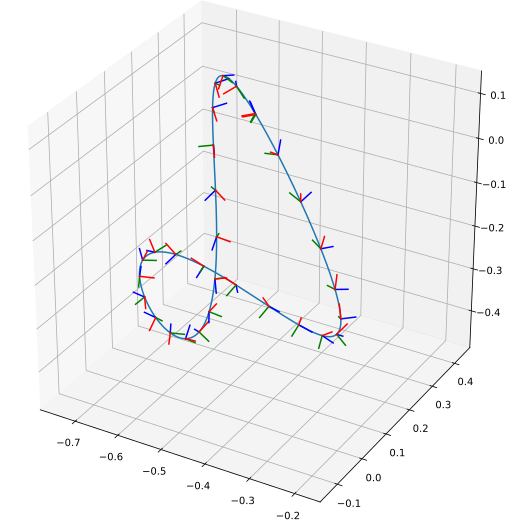
\includegraphics[width=0.8\textwidth]{figs_part2/benchmark_simulations/example_intial_rod_config}
        \caption{An example of a random initial configuration of the Cosserat rod generated by the outlined procedure. The blue line is the center-line $\mathbf{r}(u)$ and the red, green and blue lines attached to the center-line are $\mathbf{e}_1(u)$, $\mathbf{e}_2(u)$ and $\mathbf{e}_3(u)$ respectively.}
        \label{fig:example random initial cosserat configuration}
\end{figure}

This completes the description of the procedures used to generate the initial configurations of the Cosserat rod. See Fig.~\ref{fig:example random initial cosserat configuration} for an example of a random initial Cosserat configuration. For a given random configuration, which we will refer to via the index $\ell$, we ran simulations using the Forward-Euler (FEI), the $SE(3)$-integrator (SEI) and the simplified $SE(3)$ (SSEI) integrators for each $\Delta t \in \mathcal{T}$. Let $X^{I,\Delta t,\ell}$ be the result of a simulation using a given algorithm $I \in \{ \text{FEI}, \text{SEI}, \text{SSEI} \}$, time-step $\Delta t$ and initial configuration $\ell$. Using the algorithm described in App.~\ref{app:Reconstructing the Cosserat rod from xi} we can then reconstruct the corresponding spatio-temporal configuration $\Phi_\ell^{I,\Delta t,\ell} = (\mathbf{r}_\ell^{I, \Delta t,\ell} ; E_\ell^{I, \Delta t,\ell})$. We now define
\begin{subequations}
	\begin{align}
		\text{err}_\text{close}^{I, \Delta t, \ell} & = 
			|\mathbf{r}^{I, \Delta t, \ell}(T, 1) - \mathbf{r}^{I, \Delta t, \ell}(T, 0)|
			+ \sum_i |\mathbf{e}_i^{I, \Delta t, \ell}(T, 1) - \mathbf{e}_i^{I, \Delta t, \ell}(T, 0)|   \label{eq:cosserat close error}
	\end{align}
\end{subequations}
which measures the failure of the Cosserat rod to close. That is, $\text{err}_\text{close}^{I, \Delta t, \ell}$ is the magnitude of the discontinuity of $\Phi_\ell^{I,\Delta t,\ell}$ at $u=1$. As the initial configuration is a closed loop, we have $\mathbf{r}^{I, \Delta t, \ell}(0, 0) = \mathbf{r}^{I, \Delta t, \ell}(0, 1)$ for all simulations. Simulation errors will however in general cause the configuration of the Cosserat rod in the numerics to no longer close. Note that it is not sufficient for $X^{I,\Delta t,\ell}(t,u)$ to be a smooth periodic function of $u$ in order for $\Phi_\ell^{I,\Delta t,\ell}$ to be smooth a smooth function of $u$.

For both the underdamped and overdampded Cosserat rod, and for each $I$ and $\Delta t$ we ran $N_\text{sim} = 50$ simulations with random initial conditions $\ell = 1,\dots, N_\text{sim}$. We then computed the sample means and variances of the error
\begin{subequations}
	\begin{align}
		\langle \text{err}_\text{close}^{I, \Delta t} \rangle & = \frac{1}{N_\text{sim}} \sum_{\ell = 1}^{N_\text{sim}} \text{err}_\text{close}^{I, \Delta t, \ell} \\
		\text{Var}( \text{err}_\text{close}^{I, \Delta t}) & = \frac{1}{N_\text{sim}-1} \sum_{\ell = 1}^{N_\text{sim}} ( \text{err}_\text{close}^{I, \Delta t, \ell} - \langle \text{err}_\text{close}^{I, \Delta t} \rangle)^2.
	\end{align}
\end{subequations}

\begin{comment}
This completes the description of the procedures used to generate the initial configurations of the Cosserat rod. See Fig.~\ref{fig:example random initial cosserat configuration} for an example of a random initial Cosserat configuration. For a given random configuration, which we will refer to via the index $\ell$, we ran simulations using the Forward-Euler (FEI), the $SE(3)$-integrator (SEI) and the simplified $SE(3)$ (SSEI) integrators for each $\Delta t \in \mathcal{T}$. We also ran a reference simulation using the $SE(3)$-integrator at time-step $\Delta t_\text{ref} = 10^{-8}$. Let $X^{I,\Delta t,\ell}$ be the result of a simulation using a given algorithm $I \in \{ \text{FEI}, \text{SEI}, \text{SSEI} \}$, time-step $\Delta t$ and initial configuration $\ell$. Using the algorithm described in App.~\ref{app:Reconstructing the Cosserat rod from xi} we can then reconstruct the corresponding spatio-temporal configuration $\Phi_\ell^{I,\Delta t,\ell} = (\mathbf{r}_\ell^{I, \Delta t,\ell} ; E_\ell^{I, \Delta t,\ell})$. We now define
\begin{subequations}
	\begin{align}
		\text{err}_\text{ref}^{I, \Delta t, \ell} & = \sup_{i = 1, \dots, N_u} \left| \Phi_\ell^{I, \Delta t, \ell}(T, i \Delta u) - \Phi_\ell^{I, \Delta t_\text{ref}, \ell}(T, i \Delta u) \right| \label{eq:cosserat ref error} \\
		\text{err}_\text{close}^{I, \Delta t, \ell} & = |\mathbf{r}^{I, \Delta t, \ell}(T, 1) - \mathbf{r}^{I, \Delta t, \ell}(T, 0)|  \label{eq:cosserat close error}
	\end{align}
\end{subequations}
where we have defined $|\Phi| = |\mathbf{r}| + \sum_{i=1}^3 |\mathbf{e}_i|$. Equation \ref{eq:cosserat ref error} is the supremum over the residuals between the reference configuration $\Phi_\ell^{I, \Delta t_\text{ref}}$ and the $\Phi_\ell^{I, \Delta t}$. Equation \ref{eq:cosserat close error} measures the the difference between the initial and final point of the center-line. As the initial configuration is a closed loop, we have $\mathbf{r}^{I, \Delta t, \ell}(0, 0) = \mathbf{r}^{I, \Delta t, \ell}(0, 1)$ for all simulations. Numerical errors can however cause the loop to become unclosed.


For both the underdamped and overdampded Cosserat rod, and for each $I$ and $\Delta t$ we ran $N_\text{sim} = 50$ simulations with random initial conditions $\ell = 1,\dots, N_\text{sim}$. We then computed the sample mean and variances of the errors
\begin{subequations}
	\begin{align}
		\langle \text{err}_\text{ref}^{I, \Delta t} \rangle & = \frac{1}{N_\text{sim}} \sum_{\ell = 1}^{N_\text{sim}} \text{err}_\text{ref}^{I, \Delta t, \ell} \\
		\text{Var}( \text{err}_\text{ref}^{I, \Delta t}) & = \frac{1}{N_\text{sim}-1} \sum_{\ell = 1}^{N_\text{sim}} ( \text{err}_\text{ref}^{I, \Delta t, \ell} - \langle \text{err}_\text{ref}^{I, \Delta t} \rangle)^2.
	\end{align}
\end{subequations}
and
\begin{subequations}
	\begin{align}
		\langle \text{err}_\text{close}^{I, \Delta t} \rangle & = \frac{1}{N_\text{sim}} \sum_{\ell = 1}^{N_\text{sim}} \text{err}_\text{close}^{I, \Delta t, \ell} \\
		\text{Var}( \text{err}_\text{close}^{I, \Delta t}) & = \frac{1}{N_\text{sim}-1} \sum_{\ell = 1}^{N_\text{sim}} ( \text{err}_\text{close}^{I, \Delta t, \ell} - \langle \text{err}_\text{close}^{I, \Delta t} \rangle)^2.
	\end{align}
\end{subequations}
\end{comment}

\section{Simulation of the Cosserat surface}

We simulated the kinematic equations of motion of a Cosserat surface, which were given in Eq.~\ref{eq:cosserat surface eom}. We discretised space and time as
\begin{subequations}
	\begin{align} 
		u_i & = 1 - \cos \left( \frac{i \pi}{N} \right),\ i = 0, 1, \dots, N_u \label{eq:chebyshev nodes} \\
		v_i & = 1 - \cos \left( \frac{i \pi}{N} \right),\ i = 0, 1, \dots, N_v  \\
		t_i & = i \Delta t
	\end{align}
\end{subequations}
where Eq.~\ref{eq:chebyshev nodes} are known as the \textit{Chebyshev points}.\footnote{Eq.~\ref{eq:chebyshev nodes} is however in a non-standard form, as we have ordered the points in ascending order.} We differentiated functions on Chebyshev grids using \textit{spectral differentiation}, see \citep{trefethen2000spectral} for details. For all numerics we used $N_u = N_v = 20$.

To test our suite of integrators we evaluated their short-time propagators using a range of time-discretisations
\begin{equation} \label{eq:cosserat surface dts}
	\Delta t \in \mathcal{T} = \left\{ a 10^{-b}\ :\ a \in \{1, 1.25, 2, 2.5, 5 \} \text{ and } b \in \{ 4, \dots, 7 \} \right\}.
\end{equation}

Every short-term propagator was evaluated on the same initial condition $X_{0,\alpha}(u,v) = \{ \vec{\theta}_{0,\alpha}, \vec{\pi}_{0,\alpha} \},\ \alpha=u,v$, where
\begin{subequations}
	\begin{align}
		(\theta_{0,u})_2(i\Delta u, j \Delta u) & = 1 \\
		(\theta_{0,u})_1(i\Delta u, j \Delta u) & = (\theta_{0,u})_3(i\Delta u, j \Delta u) = 0 \\
		(\theta_{0,v})_3(i\Delta u, j \Delta u) & = 1 \\
		(\theta_{0,v})_1(i\Delta u, j \Delta u) & = (\theta_{0,v})_2(i\Delta u, j \Delta u) = 0 \\
		\vec{\pi}_{0,u}(i\Delta u, j \Delta u) & = \vec{\pi}_{0,v}(i\Delta u, j \Delta u) = 0
	\end{align}
\end{subequations}
for all $i = 0,\dots, N_u,\ j=0,\dots,N_v$. The corresponding spatio-temporal configuration $\Phi_0 = (\mathbf{r}, E)$ is a flat sheet $\mathbf{r}(i \Delta u, j \Delta u)  = (0, i \Delta u, j \Delta v )^T$ with a constant perpendicular material frame. The system is subject to generalised velocity field $N_0 = \{ \vec{V}_0, \vec{\Omega}_0 \}$ which we generate as a random superposition of sinusoidal surfaces, which can reproduces using Listing \ref{lst:cosserat surface initial conditions}.

\begin{lstlisting}[language=Python, caption=Setting up initial conditions nad generating random velocity fields., label={lst:cosserat surface initial conditions}]
# Parameters

Lu0 = 1
Lv0 = 1

Nu = 20
Nv = 20

N_rand_V_u = 5
N_rand_V_v = 5

N_rand_Omg_u = 5
N_rand_Omg_v = 5

rand_V_var = 1e0
rand_Omg_var = 1e0

# Initial conditions

thu0 = np.zeros((3, Nu, Nv))
thv0 = np.zeros((3, Nu, Nv))
piu0 = np.zeros((3, Nu, Nv))
piv0 = np.zeros((3, Nu, Nv))

thu0[1] = 1
thv0[2] = 1

piu0[1] = 0
piv0[0] = 0

# Construct material mesh grid

def get_grid_1D(Mm, L):
    N = Mm - 1
    x = np.cos(np.pi*np.arange(0,N+1)/N)
    x = L*(1-x)/2
    return x

us = get_grid_1D(Nu, Lu0)
vs = get_grid_1D(Nv, Lv0)
grid_U, grid_V = np.meshgrid(us, vs, indexing='ij')

# Define random velocity and and angular velocity

rand_V_coeffs = np.zeros((3, N_rand_V_u, N_rand_V_v))
rand_Omg_coeffs = np.zeros((3, N_rand_Omg_u, N_rand_Omg_v))

for di in range(dim):
    for i in range(N_rand_V_u):
        for j in range(N_rand_V_v):
            rand_V_coeffs[di,i,j] = rand_V_var * np.random.normal()
            rand_Omg_coeffs[di,i,j] = rand_Omg_var * np.random.normal()
            
# Compute velocity field

V_field = np.zeros((3, Nu, Nv))
for di in range(dim):
    for i in range(N_rand_V_u):
        for j in range(N_rand_V_v):
            V_field[di] += rand_V_coeffs[di,i,j] * np.sin((i - 0.5)*np.pi*grid_U/Lu0) * np.sin((j - 0.5)*np.pi*grid_V/Lv0) / ( (i-0.5) * (j - 0.5) * np.pi**2 )

# Compute angular velocity field

Omg_field = np.zeros((3, Nu, Nv))
for di in range(dim):
    for i in range(N_rand_Omg_u):
        for j in range(N_rand_Omg_v):
            Omg_field[di] += rand_Omg_coeffs[di,i,j] * np.sin((i - 0.5)*np.pi*grid_U/Lu0) * np.sin((j - 0.5)*np.pi*grid_V/Lv0) / ( (i-0.5) * (j - 0.5) * np.pi**2 )
\end{lstlisting}

Let $I \in \{ \text{FEI}, \text{SEI}, \text{SSEI} \}$ refer to the Forward-Euler, $SE(3)$- and simplified $SE(3)$-propagators respectively, and let $\ell = 1, \dots, N_\text{sim}$ be an index over the set of randomly generated velocity fields. In our results we used $N_\text{sim} = 50$. Let $X_{\Delta t, \alpha}^{I, \ell}$ be the result of computing the short-term propagator using integrator $I$, with time-step $\Delta t$ and configuration $\ell$. For each $I$, $\Delta t$ and $\ell$, we computed the supremum of the residual integrability error $\Delta^\text{int}_{u v}$, given in Eq.~\ref{eq:spatial integrability residual} over the material base space. In other words we compute
\begin{equation}
	\text{err}_\text{int}^{I, \Delta t, \ell} = \sup_{ i = 1,\dots,N_u,\ j = 1,\dots, N_v } \left| \partial_v X_{\Delta t, u}^{I, \ell} (i \Delta u, j \Delta v) - \mathcal{D}_u X_{\Delta t, v}^{I, \ell} (i \Delta u, j \Delta v).
 \right|
\end{equation}
where the derivatives were computed on the Chebyshev grid using spectral differentiation. We also compute the mean and variance of the integrability error over the set of configurations $\ell$
\begin{subequations}
	\begin{align}
		\langle \text{err}_\text{int}^{I, \Delta t} \rangle & = \frac{1}{N_\text{sim}} \sum_{\ell = 1}^{N_\text{sim}} \text{err}_\text{int}^{I, \Delta t, \ell} \\
		\text{Var}( \text{err}_\text{int}^{I, \Delta t}) & = \frac{1}{N_\text{sim}-1} \sum_{\ell = 1}^{N_\text{sim}} ( \text{err}_\text{int}^{I, \Delta t, \ell} - \langle \text{err}_\text{ref}^{I, \Delta t} \rangle)^2.
	\end{align}
\end{subequations}



\begin{comment}
\chapter*{Notation} \label{app:glossary of notation}
\addcontentsline{toc}{chapter}{Notation}

%Vectors will be denoted in both as $\mathbf{v}$ and $\vec{v}$, with components $v_i$. We write the Euclidean norm of a vector as $|\mathbf{v}| = |\vec{v}|$. 


Functions $f$ are maps $f : A \to B$, where $A$ and $B$ are the domain and codomain of the function respectively. If $a \in A$ then $f(a) \in B$. We denote and define the image of a function as $f(A) = \{ f(a)\ :\ a \in B \}$. We denote that a map $f : \mathbb{R} \to \mathbb{R}$ is $k$-times differentiable as $f \in C^k$. The function $f$ is continuous if $f \in C^0$, and smooth if $f \in C^\infty$. This extends to functions on $\mathbb{R}^d$.

\section*{Notation specific to Part I}



Measure, density, law




$C^0_{\mathbf{x}_0}([0,T])$




Let $P$ be the probability density of $\mathbb{P}$ with respect to the Lebesgue measure, and we will henceforth write this relation as $P \sim \mathbb{P}$.


$(Z_i)_j \sim \mathcal{N}(0, 2D)$

$\mathcal{N}(0, \mathbbm{1}_d)$

$\mathcal{N}(0, \mathcal{C})$ for infinite dimensional operators.s

$\langle X \rangle $


$\langle\mathbf{f},\mathbf{g}\rangle=\sum_{i}\int_{0}^{T}f_{i}(t)g_{i}(t)dt$

\section*{Part II notation}

Euclidean vectors are written in boldface as $\mathbf{v} \in \mathbb{E}^d$, where $\mathbb{E}^d$ is $d$-dimensional Euclidean space, with inner product $\mathbf{v} \cdot \mathbf{w}$ for $\mathbf{w} \in \mathbb{E}^d$. We write column vectors as $\vec{v} \in \mathbb{R}^d$, with components $\vec{v} = (v_1\ v_2\ \dots\ v_d)^T$.
  

Matrix derivatives are carried out using the numerator-layout convention. For a matrix $X \in \mathbb{R}^{p \times q}$ and $y(X)$ a scalar function, then
\begin{equation} \label{eq:numerator-layout convention}
	\frac{\partial y}{\partial X} = \begin{pmatrix}
		\frac{\partial y}{\partial X_{11}} & \frac{\partial y}{\partial X_{21}} & \dots & \frac{\partial y}{\partial X_{p1}} \\
		\frac{\partial y}{\partial X_{12}} & \frac{\partial y}{\partial X_{22}} & \dots & \frac{\partial y}{\partial X_{p2}} \\
		 \vdots & \ddots & \vdots \\
		 \frac{\partial y}{\partial X_{1q}} & \frac{\partial y}{\partial X_{2q}} & \dots & \frac{\partial y}{\partial X_{pq}}
	\end{pmatrix}
\end{equation}.
For $\vec{x} \in \mathbb{R}^d$
\begin{equation}
	\frac{\partial y}{\partial \vec{x}} = \begin{pmatrix}
		\frac{\partial y}{\partial x_1} \\
		\frac{\partial y}{\partial x_2} \\
		\vdots \\
		\frac{\partial y}{\partial x_p}
	\end{pmatrix}
\end{equation}

Often we will abbreviate partial derivatives as
\begin{equation}
\begin{aligned}
\partial_u f & := \frac{\partial f}{\partial u} \\
\partial_t f & := \frac{\partial f}{\partial t}
\end{aligned}
\end{equation}
or
\begin{equation}
\begin{aligned}
f' & := \frac{\partial f}{\partial u} \\
\dot{f} & := \frac{\partial f}{\partial t}
\end{aligned}.
\end{equation}
This applies to both scalar, vectorial and group-valued functions. 

If we have multiple coordinates, derivatives will be denoted by subscripts i.e. $f_u$, $f_t$ etc. or $\partial_\alpha = \frac{\partial}{\partial u^\alpha}$.

In any dimension $d$ we will assume that $\mathbb{R}^d$ is a vector space equipped with the standard Euclidean metric. Vectors $\mathbf{a} \in \mathbb{R}^d$ will be written as column vectors $\mathbf{a} = (a_1\ a_2\ \dots\ a_d)^T$, and their inner product will often be written as
\begin{equation}
\mathbf{a} \cdot \mathbf{b} = \mathbf{a}^T \mathbf{b}
\end{equation}
interchangeably.

which for any two vectors $\mathbf{a},\mathbf{b}\in \mathbb{R}^d$ can be written in several different ways interchangeably:
\begin{equation}
\mathbf{a} \cdot \mathbf{b} = \mathbf{a}^T \mathbf{b}
\end{equation}


We will often distinguish $\mathbb{E}^d$ and $\mathbb{R}^d$. 



Introduce the vec notation here as well, and tilde notation $\tilde{v}$, and do it clearly and in detail.

$e$ is the identity of Lie groups.

introduce the hatmap and give it explicitly (and use the vec notation). 

\begin{equation} \label{eq:hat map}
\hat{v} =  \begin{pmatrix}
0 & -v_3 & v_2 \\
v_3 & 0 & - v_1 \\
- v_2 & v_1 & 0
\end{pmatrix}
\end{equation}

also have that $\vec{\cdot}$ signifes the inverse hatmap for anti-symmetric 3x3 matrices. So $\vec{\hat{v}} \in \mathbb{R}^{3}$.

$\hat{v} = v \times$

$x \times y = - y \times x =  \hat{y} x$

$\mathbb{1}$ identity matrix



$X = \{ \vec{a} ; \vec{b} \}$


Matrix derivatives, and the fact that we only take them with respect to the non-zero values. $A_{ji} = \frac{\partial U}{\partial B_{ij}}$.

$\bigwedge_{\beta \neq \alpha}$

closure of sets $\bar{U}$.



\begin{equation}
	\{ \vec{a}, \vec{m} \} = \begin{pmatrix}
		0 & \vec{0}^T \\
		\vec{a} & \hat{m}
	\end{pmatrix} \in \mathfrak{se}(3)
\end{equation}
where $\vec{a}, \vec{m} \in \mathbb{R}^3$, and $\vec{0} = (0\ 0\ 0)^T$.
\begin{equation}
	\{ \vec{b}, \vec{n} \}^* = \begin{pmatrix}
		0 & \vec{b}^T \\
		\vec{0} & \hat{n}^T
	\end{pmatrix} \in \mathfrak{se}^*(3)
\end{equation}
where $\vec{b}, \vec{n} \in \mathbb{R}^3$

\end{comment}


%\end{appendices}

%%%%%%%%%%%%%%%%%%%%%%%%%%%%%%%%%%%%%%%%%%%%%%%%%%%%%%%%%%%%%%%%%%%%%%%%%%%%%%%%
%% Index:
%%
%\printthesisindex

\end{document}
